\documentclass[twoside]{book}

% Packages required by doxygen
\usepackage{fixltx2e}
\usepackage{calc}
\usepackage{doxygen}
\usepackage[export]{adjustbox} % also loads graphicx
\usepackage{graphicx}
\usepackage[utf8]{inputenc}
\usepackage{makeidx}
\usepackage{multicol}
\usepackage{multirow}
\PassOptionsToPackage{warn}{textcomp}
\usepackage{textcomp}
\usepackage[nointegrals]{wasysym}
\usepackage[table]{xcolor}

% Font selection
\usepackage[T1]{fontenc}
\usepackage[scaled=.90]{helvet}
\usepackage{courier}
\usepackage{amssymb}
\usepackage{sectsty}
\renewcommand{\familydefault}{\sfdefault}
\allsectionsfont{%
  \fontseries{bc}\selectfont%
  \color{darkgray}%
}
\renewcommand{\DoxyLabelFont}{%
  \fontseries{bc}\selectfont%
  \color{darkgray}%
}
\newcommand{\+}{\discretionary{\mbox{\scriptsize$\hookleftarrow$}}{}{}}

% Page & text layout
\usepackage{geometry}
\geometry{%
  letterpaper,%
  top=2.5cm,%
  bottom=2.5cm,%
  left=2.5cm,%
  right=2.5cm%
}
\tolerance=750
\hfuzz=15pt
\hbadness=750
\setlength{\emergencystretch}{15pt}
\setlength{\parindent}{0cm}
\setlength{\parskip}{3ex plus 2ex minus 2ex}
\makeatletter
\renewcommand{\paragraph}{%
  \@startsection{paragraph}{4}{0ex}{-1.0ex}{1.0ex}{%
    \normalfont\normalsize\bfseries\SS@parafont%
  }%
}
\renewcommand{\subparagraph}{%
  \@startsection{subparagraph}{5}{0ex}{-1.0ex}{1.0ex}{%
    \normalfont\normalsize\bfseries\SS@subparafont%
  }%
}
\makeatother

% Headers & footers
\usepackage{fancyhdr}
\pagestyle{fancyplain}
\fancyhead[LE]{\fancyplain{}{\bfseries\thepage}}
\fancyhead[CE]{\fancyplain{}{}}
\fancyhead[RE]{\fancyplain{}{\bfseries\leftmark}}
\fancyhead[LO]{\fancyplain{}{\bfseries\rightmark}}
\fancyhead[CO]{\fancyplain{}{}}
\fancyhead[RO]{\fancyplain{}{\bfseries\thepage}}
\fancyfoot[LE]{\fancyplain{}{}}
\fancyfoot[CE]{\fancyplain{}{}}
\fancyfoot[RE]{\fancyplain{}{\bfseries\scriptsize Generated by Doxygen }}
\fancyfoot[LO]{\fancyplain{}{\bfseries\scriptsize Generated by Doxygen }}
\fancyfoot[CO]{\fancyplain{}{}}
\fancyfoot[RO]{\fancyplain{}{}}
\renewcommand{\footrulewidth}{0.4pt}
\renewcommand{\chaptermark}[1]{%
  \markboth{#1}{}%
}
\renewcommand{\sectionmark}[1]{%
  \markright{\thesection\ #1}%
}

% Indices & bibliography
\usepackage{natbib}
\usepackage[titles]{tocloft}
\setcounter{tocdepth}{3}
\setcounter{secnumdepth}{5}
\makeindex

% Hyperlinks (required, but should be loaded last)
\usepackage{ifpdf}
\ifpdf
  \usepackage[pdftex,pagebackref=true]{hyperref}
\else
  \usepackage[ps2pdf,pagebackref=true]{hyperref}
\fi
\hypersetup{%
  colorlinks=true,%
  linkcolor=blue,%
  citecolor=blue,%
  unicode%
}

% Custom commands
\newcommand{\clearemptydoublepage}{%
  \newpage{\pagestyle{empty}\cleardoublepage}%
}

\usepackage{caption}
\captionsetup{labelsep=space,justification=centering,font={bf},singlelinecheck=off,skip=4pt,position=top}

%===== C O N T E N T S =====

\begin{document}

% Titlepage & ToC
\hypersetup{pageanchor=false,
             bookmarksnumbered=true,
             pdfencoding=unicode
            }
\pagenumbering{alph}
\begin{titlepage}
\vspace*{7cm}
\begin{center}%
{\Large Layout Control System (L\+CS) }\\
\vspace*{1cm}
{\large Generated by Doxygen 1.8.13}\\
\end{center}
\end{titlepage}
\clearemptydoublepage
\pagenumbering{roman}
\tableofcontents
\clearemptydoublepage
\pagenumbering{arabic}
\hypersetup{pageanchor=true}

%--- Begin generated contents ---
\chapter{Layout Control System (L\+CS)}
\label{index}\hypertarget{index}{}A project that uses E\+S\+P8266 Wi\+Fi modules that communicate with a Raspberry Pi server to control accessories on the Garfield-\/\+Clarendon Model Railroad Club.

\subsubsection*{Prerequisites}

The code running on the E\+S\+P8266 is developed using the Arduino I\+DE

The L\+C\+S\+Server application running on the Raspberry Pi makes use of the Qt framework. The E\+S\+P8266 uses http calls to communicate with the L\+C\+S\+Server application and U\+DP unicast messages to communicate with other E\+S\+P8266 controllers on the layout. A separate R\+E\+S\+Tful A\+PI provides access to commands to activate routes, set turnouts and update data in the configuration database.

\href{https://github.com/garfieldclarendon/ardunio/api/index.html}{\tt A\+PI Reference}

\subsection*{Built With}


\begin{DoxyItemize}
\item \href{https://www.arduino.cc/en/Main/Software}{\tt Arduino} -\/ Arduino Tools
\item \href{https://www.qt.io/}{\tt Qt} -\/ Qt Framework
\end{DoxyItemize}

\subsection*{Contributing}

Please read \href{https://gist.github.com/PurpleBooth/b24679402957c63ec426}{\tt C\+O\+N\+T\+R\+I\+B\+U\+T\+I\+N\+G.\+md} for details on our code of conduct, and the process for submitting pull requests to us.

\subsection*{Authors}


\begin{DoxyItemize}
\item {\bfseries John Reilly} -\/ {\itshape Initial work}
\end{DoxyItemize}

\subsection*{License}

This project is licensed under the M\+IT License -\/ see the L\+I\+C\+E\+N\+SE.md file for details 
\chapter{Module Index}
\section{Modules}
Here is a list of all modules\+:\begin{DoxyCompactList}
\item \contentsline{section}{U\+DP Message I\+Ds}{\pageref{group___u_d_p_message_i_d}}{}
\end{DoxyCompactList}

\chapter{Hierarchical Index}
\section{Class Hierarchy}
This inheritance list is sorted roughly, but not completely, alphabetically\+:\begin{DoxyCompactList}
\item \contentsline{section}{Address\+Struct}{\pageref{struct_address_struct}}{}
\item \contentsline{section}{Address\+Union}{\pageref{union_address_union}}{}
\item \contentsline{section}{A\+P\+I\+Request}{\pageref{class_a_p_i_request}}{}
\item \contentsline{section}{A\+P\+I\+Response}{\pageref{class_a_p_i_response}}{}
\item \contentsline{section}{Controller\+Entry}{\pageref{class_controller_entry}}{}
\item \contentsline{section}{Device\+Status}{\pageref{class_device_status}}{}
\item \contentsline{section}{I\+P4\+Address\+Union}{\pageref{union_i_p4_address_union}}{}
\item \contentsline{section}{Message\+Device\+Struct}{\pageref{struct_message_device_struct}}{}
\item \contentsline{section}{N\+C\+E\+Message}{\pageref{class_n_c_e_message}}{}
\item \contentsline{section}{Payload\+Union}{\pageref{union_payload_union}}{}
\item Q\+Dialog\begin{DoxyCompactList}
\item \contentsline{section}{Status\+Dialog}{\pageref{class_status_dialog}}{}
\end{DoxyCompactList}
\item Q\+Object\begin{DoxyCompactList}
\item \contentsline{section}{A\+P\+I\+Controller}{\pageref{class_a_p_i_controller}}{}
\item \contentsline{section}{A\+P\+I\+Device}{\pageref{class_a_p_i_device}}{}
\item \contentsline{section}{A\+P\+I\+Entity}{\pageref{class_a_p_i_entity}}{}
\item \contentsline{section}{A\+P\+I\+Route}{\pageref{class_a_p_i_route}}{}
\item \contentsline{section}{A\+P\+I\+Signal}{\pageref{class_a_p_i_signal}}{}
\item \contentsline{section}{A\+P\+I\+Turnout}{\pageref{class_a_p_i_turnout}}{}
\item \contentsline{section}{App\+Service}{\pageref{class_app_service}}{}
\item \contentsline{section}{Controller\+Manager}{\pageref{class_controller_manager}}{}
\item \contentsline{section}{Database}{\pageref{class_database}}{}
\item \contentsline{section}{Device\+Handler}{\pageref{class_device_handler}}{}
\item \contentsline{section}{Device\+Manager}{\pageref{class_device_manager}}{}
\item \contentsline{section}{Entity\+Metadata}{\pageref{class_entity_metadata}}{}
\item \contentsline{section}{Message\+Broadcaster}{\pageref{class_message_broadcaster}}{}
\item \contentsline{section}{N\+C\+E\+Interface}{\pageref{class_n_c_e_interface}}{}
\item \contentsline{section}{Notification\+Server}{\pageref{class_notification_server}}{}
\item \contentsline{section}{P\+I\+G\+P\+IO}{\pageref{class_p_i_g_p_i_o}}{}
\item \contentsline{section}{Qt\+Service\+Controller\+Handler}{\pageref{class_qt_service_controller_handler}}{}
\item \contentsline{section}{Qt\+Service\+Starter}{\pageref{class_qt_service_starter}}{}
\item \contentsline{section}{Simulator}{\pageref{class_simulator}}{}
\item \contentsline{section}{Url\+Handler}{\pageref{class_url_handler}}{}
\end{DoxyCompactList}
\item Q\+Tcp\+Server\begin{DoxyCompactList}
\item \contentsline{section}{Qt\+Unix\+Server\+Socket}{\pageref{class_qt_unix_server_socket}}{}
\begin{DoxyCompactList}
\item \contentsline{section}{Qt\+Service\+Sys\+Private}{\pageref{class_qt_service_sys_private}}{}
\end{DoxyCompactList}
\item \contentsline{section}{Web\+Server}{\pageref{class_web_server}}{}
\end{DoxyCompactList}
\item Q\+Tcp\+Socket\begin{DoxyCompactList}
\item \contentsline{section}{Qt\+Unix\+Socket}{\pageref{class_qt_unix_socket}}{}
\end{DoxyCompactList}
\item Q\+Thread\begin{DoxyCompactList}
\item \contentsline{section}{Handler\+Thread}{\pageref{class_handler_thread}}{}
\item \contentsline{section}{Serial\+Port\+Thread}{\pageref{class_serial_port_thread}}{}
\item \contentsline{section}{Web\+Server\+Thread}{\pageref{class_web_server_thread}}{}
\end{DoxyCompactList}
\item \contentsline{section}{Qt\+Service\+Base}{\pageref{class_qt_service_base}}{}
\begin{DoxyCompactList}
\item \contentsline{section}{Qt\+Service$<$ Application $>$}{\pageref{class_qt_service}}{}
\item \contentsline{section}{Qt\+Service$<$ Q\+Core\+Application $>$}{\pageref{class_qt_service}}{}
\begin{DoxyCompactList}
\item \contentsline{section}{App\+Service}{\pageref{class_app_service}}{}
\end{DoxyCompactList}
\end{DoxyCompactList}
\item \contentsline{section}{Qt\+Service\+Base\+Private}{\pageref{class_qt_service_base_private}}{}
\item \contentsline{section}{Qt\+Service\+Controller}{\pageref{class_qt_service_controller}}{}
\item \contentsline{section}{Qt\+Service\+Controller\+Private}{\pageref{class_qt_service_controller_private}}{}
\item \contentsline{section}{U\+D\+P\+Message}{\pageref{class_u_d_p_message}}{}
\item \contentsline{section}{U\+D\+P\+Message\+Struct}{\pageref{struct_u_d_p_message_struct}}{}
\end{DoxyCompactList}

\chapter{Class Index}
\section{Class List}
Here are the classes, structs, unions and interfaces with brief descriptions\+:\begin{DoxyCompactList}
\item\contentsline{section}{\hyperlink{struct_address_struct}{Address\+Struct} }{\pageref{struct_address_struct}}{}
\item\contentsline{section}{\hyperlink{union_address_union}{Address\+Union} }{\pageref{union_address_union}}{}
\item\contentsline{section}{\hyperlink{class_a_p_i_controller}{A\+P\+I\+Controller} \\*A\+PI handler class for a L\+CS controller. This class handles all A\+PI requests for a controller. Two types of requests are made as it relates to a L\+CS controller; \char`\"{}/\+A\+P\+I/...\char`\"{} requests sent from an external source like a web page or an application and a \char`\"{}/controller/...\char`\"{} requests sent by a L\+CS controller to download information from the application server }{\pageref{class_a_p_i_controller}}{}
\item\contentsline{section}{\hyperlink{class_a_p_i_entity}{A\+P\+I\+Entity} \\*A\+PI handler class for L\+CS database entities. This class handles basic database fetch and C\+R\+UD operations (Create, Update and Delete). See the A\+PI documentation for more information }{\pageref{class_a_p_i_entity}}{}
\item\contentsline{section}{\hyperlink{class_a_p_i_handler}{A\+P\+I\+Handler} }{\pageref{class_a_p_i_handler}}{}
\item\contentsline{section}{\hyperlink{class_a_p_i_request}{A\+P\+I\+Request} }{\pageref{class_a_p_i_request}}{}
\item\contentsline{section}{\hyperlink{class_a_p_i_response}{A\+P\+I\+Response} }{\pageref{class_a_p_i_response}}{}
\item\contentsline{section}{\hyperlink{class_block_handler}{Block\+Handler} }{\pageref{class_block_handler}}{}
\item\contentsline{section}{\hyperlink{class_c_app_service}{C\+App\+Service} }{\pageref{class_c_app_service}}{}
\item\contentsline{section}{\hyperlink{class_controller_entry}{Controller\+Entry} }{\pageref{class_controller_entry}}{}
\item\contentsline{section}{\hyperlink{class_controller_manager}{Controller\+Manager} }{\pageref{class_controller_manager}}{}
\item\contentsline{section}{\hyperlink{class_controller_message}{Controller\+Message} }{\pageref{class_controller_message}}{}
\item\contentsline{section}{\hyperlink{class_database}{Database} }{\pageref{class_database}}{}
\item\contentsline{section}{\hyperlink{class_device_handler}{Device\+Handler} }{\pageref{class_device_handler}}{}
\item\contentsline{section}{\hyperlink{class_device_manager}{Device\+Manager} }{\pageref{class_device_manager}}{}
\item\contentsline{section}{\hyperlink{class_device_status}{Device\+Status} }{\pageref{class_device_status}}{}
\item\contentsline{section}{\hyperlink{class_entity_metadata}{Entity\+Metadata} }{\pageref{class_entity_metadata}}{}
\item\contentsline{section}{\hyperlink{class_handler_thread}{Handler\+Thread} }{\pageref{class_handler_thread}}{}
\item\contentsline{section}{\hyperlink{union_i_p4_address_union}{I\+P4\+Address\+Union} }{\pageref{union_i_p4_address_union}}{}
\item\contentsline{section}{\hyperlink{class_message_broadcaster}{Message\+Broadcaster} }{\pageref{class_message_broadcaster}}{}
\item\contentsline{section}{\hyperlink{class_n_c_e_interface}{N\+C\+E\+Interface} }{\pageref{class_n_c_e_interface}}{}
\item\contentsline{section}{\hyperlink{class_n_c_e_message}{N\+C\+E\+Message} }{\pageref{class_n_c_e_message}}{}
\item\contentsline{section}{\hyperlink{class_notification_server}{Notification\+Server} }{\pageref{class_notification_server}}{}
\item\contentsline{section}{\hyperlink{class_panel_handler}{Panel\+Handler} }{\pageref{class_panel_handler}}{}
\item\contentsline{section}{\hyperlink{class_p_i_g_p_i_o}{P\+I\+G\+P\+IO} }{\pageref{class_p_i_g_p_i_o}}{}
\item\contentsline{section}{\hyperlink{class_qt_service}{Qt\+Service$<$ Application $>$} \\*The \hyperlink{class_qt_service}{Qt\+Service} is a convenient template class that allows you to create a service for a particular application type }{\pageref{class_qt_service}}{}
\item\contentsline{section}{\hyperlink{class_qt_service_base}{Qt\+Service\+Base} \\*A\+PI for implementing Windows services and Unix daemons }{\pageref{class_qt_service_base}}{}
\item\contentsline{section}{\hyperlink{class_qt_service_base_private}{Qt\+Service\+Base\+Private} }{\pageref{class_qt_service_base_private}}{}
\item\contentsline{section}{\hyperlink{class_qt_service_controller}{Qt\+Service\+Controller} \\*Allows you to control services from separate applications }{\pageref{class_qt_service_controller}}{}
\item\contentsline{section}{\hyperlink{class_qt_service_controller_handler}{Qt\+Service\+Controller\+Handler} }{\pageref{class_qt_service_controller_handler}}{}
\item\contentsline{section}{\hyperlink{class_qt_service_controller_private}{Qt\+Service\+Controller\+Private} }{\pageref{class_qt_service_controller_private}}{}
\item\contentsline{section}{\hyperlink{class_qt_service_starter}{Qt\+Service\+Starter} }{\pageref{class_qt_service_starter}}{}
\item\contentsline{section}{\hyperlink{class_qt_service_sys_private}{Qt\+Service\+Sys\+Private} }{\pageref{class_qt_service_sys_private}}{}
\item\contentsline{section}{\hyperlink{class_qt_unix_server_socket}{Qt\+Unix\+Server\+Socket} }{\pageref{class_qt_unix_server_socket}}{}
\item\contentsline{section}{\hyperlink{class_qt_unix_socket}{Qt\+Unix\+Socket} }{\pageref{class_qt_unix_socket}}{}
\item\contentsline{section}{\hyperlink{class_route_handler}{Route\+Handler} }{\pageref{class_route_handler}}{}
\item\contentsline{section}{\hyperlink{class_semaphore_handler}{Semaphore\+Handler} }{\pageref{class_semaphore_handler}}{}
\item\contentsline{section}{\hyperlink{class_serial_port_thread}{Serial\+Port\+Thread} }{\pageref{class_serial_port_thread}}{}
\item\contentsline{section}{\hyperlink{class_signal_handler}{Signal\+Handler} }{\pageref{class_signal_handler}}{}
\item\contentsline{section}{\hyperlink{class_simulator}{Simulator} }{\pageref{class_simulator}}{}
\item\contentsline{section}{\hyperlink{class_status_dialog}{Status\+Dialog} }{\pageref{class_status_dialog}}{}
\item\contentsline{section}{\hyperlink{class_turnout_handler}{Turnout\+Handler} }{\pageref{class_turnout_handler}}{}
\item\contentsline{section}{\hyperlink{class_u_d_p_message}{U\+D\+P\+Message} \\*A class for handling U\+DP messages sent between controllers and the application server. This class along with the \hyperlink{struct_u_d_p_message_struct}{Message Structure} contains the data layout of a U\+DP message. Messages are sent from controller-\/to-\/controller in a peer-\/to-\/peer fasion using U\+DP uni-\/cast. Each controller contains a list of \char`\"{}controllers to notify\char`\"{} in its configuration data. Each time a device needs to send a command or status message, the controller\textquotesingle{}s Network Manager sends the message to all controllers contained in the notification list. Each controller listens for the \hyperlink{group___u_d_p_message_i_d_ga23aab89076591390a1dbc412a3a07314}{S\+Y\+S\+\_\+\+C\+O\+N\+T\+R\+O\+L\+L\+E\+R\+\_\+\+O\+N\+L\+I\+NE} broadcast message which is sent by each controller upon startup. Upon resceiving this message, the controller checks to see if the controller\textquotesingle{}s ID is contained in its notification list and, if so, stores the address of the sending controller which is stored in field\mbox{[}0\mbox{]} -\/ field\mbox{[}3\mbox{]} and then responds by sending device status messages. If the controller misses this message, the controller sends a \hyperlink{group___u_d_p_message_i_d_gadfda0e5a5a6a08de555dd55182a4cd87}{S\+Y\+S\+\_\+\+F\+I\+N\+D\+\_\+\+C\+O\+N\+T\+R\+O\+L\+L\+ER} broadcast message every 3 seconds for each controller in its notification list until it recieves a corresponding \hyperlink{group___u_d_p_message_i_d_ga23aab89076591390a1dbc412a3a07314}{S\+Y\+S\+\_\+\+C\+O\+N\+T\+R\+O\+L\+L\+E\+R\+\_\+\+O\+N\+L\+I\+NE} message from each controller }{\pageref{class_u_d_p_message}}{}
\item\contentsline{section}{\hyperlink{struct_u_d_p_message_struct}{U\+D\+P\+Message\+Struct} \\*Structure used the by the \hyperlink{class_u_d_p_message}{U\+D\+P\+Message} class which contains the actual data of a U\+DP Message }{\pageref{struct_u_d_p_message_struct}}{}
\item\contentsline{section}{\hyperlink{class_url_handler}{Url\+Handler} }{\pageref{class_url_handler}}{}
\item\contentsline{section}{\hyperlink{class_web_server}{Web\+Server} }{\pageref{class_web_server}}{}
\item\contentsline{section}{\hyperlink{class_web_server_thread}{Web\+Server\+Thread} }{\pageref{class_web_server_thread}}{}
\end{DoxyCompactList}

\chapter{File Index}
\section{File List}
Here is a list of all documented files with brief descriptions\+:\begin{DoxyCompactList}
\item\contentsline{section}{L\+C\+S\+Server/{\bfseries A\+P\+I\+Controller.\+h} }{\pageref{_a_p_i_controller_8h}}{}
\item\contentsline{section}{L\+C\+S\+Server/{\bfseries A\+P\+I\+Device.\+h} }{\pageref{_a_p_i_device_8h}}{}
\item\contentsline{section}{L\+C\+S\+Server/{\bfseries A\+P\+I\+Entity.\+h} }{\pageref{_a_p_i_entity_8h}}{}
\item\contentsline{section}{L\+C\+S\+Server/{\bfseries A\+P\+I\+Request.\+h} }{\pageref{_a_p_i_request_8h}}{}
\item\contentsline{section}{L\+C\+S\+Server/{\bfseries A\+P\+I\+Response.\+h} }{\pageref{_a_p_i_response_8h}}{}
\item\contentsline{section}{L\+C\+S\+Server/{\bfseries A\+P\+I\+Route.\+h} }{\pageref{_a_p_i_route_8h}}{}
\item\contentsline{section}{L\+C\+S\+Server/{\bfseries A\+P\+I\+Signal.\+h} }{\pageref{_a_p_i_signal_8h}}{}
\item\contentsline{section}{L\+C\+S\+Server/{\bfseries A\+P\+I\+Turnout.\+h} }{\pageref{_a_p_i_turnout_8h}}{}
\item\contentsline{section}{L\+C\+S\+Server/{\bfseries App\+Service.\+h} }{\pageref{_app_service_8h}}{}
\item\contentsline{section}{L\+C\+S\+Server/{\bfseries Controller\+Manager.\+h} }{\pageref{_controller_manager_8h}}{}
\item\contentsline{section}{L\+C\+S\+Server/{\bfseries Database.\+h} }{\pageref{_database_8h}}{}
\item\contentsline{section}{L\+C\+S\+Server/{\bfseries Device\+Handler.\+h} }{\pageref{_device_handler_8h}}{}
\item\contentsline{section}{L\+C\+S\+Server/{\bfseries Device\+Manager.\+h} }{\pageref{_device_manager_8h}}{}
\item\contentsline{section}{L\+C\+S\+Server/{\bfseries Entity\+Metadata.\+h} }{\pageref{_entity_metadata_8h}}{}
\item\contentsline{section}{L\+C\+S\+Server/{\bfseries Message\+Broadcaster.\+h} }{\pageref{_message_broadcaster_8h}}{}
\item\contentsline{section}{L\+C\+S\+Server/{\bfseries N\+C\+E\+Interface.\+h} }{\pageref{_n_c_e_interface_8h}}{}
\item\contentsline{section}{L\+C\+S\+Server/{\bfseries N\+C\+E\+Message.\+h} }{\pageref{_n_c_e_message_8h}}{}
\item\contentsline{section}{L\+C\+S\+Server/{\bfseries Notification\+Server.\+h} }{\pageref{_notification_server_8h}}{}
\item\contentsline{section}{L\+C\+S\+Server/{\bfseries P\+I\+G\+P\+I\+O.\+h} }{\pageref{_p_i_g_p_i_o_8h}}{}
\item\contentsline{section}{L\+C\+S\+Server/{\bfseries Simulator.\+h} }{\pageref{_simulator_8h}}{}
\item\contentsline{section}{L\+C\+S\+Server/{\bfseries Status\+Dialog.\+h} }{\pageref{_status_dialog_8h}}{}
\item\contentsline{section}{L\+C\+S\+Server/{\bfseries Web\+Server.\+h} }{\pageref{_web_server_8h}}{}
\item\contentsline{section}{L\+C\+S\+Server/{\bfseries Web\+Server\+Thread.\+h} }{\pageref{_web_server_thread_8h}}{}
\item\contentsline{section}{L\+C\+S\+Server/\+Qt\+Solutions\+Service/src/{\bfseries qtservice.\+h} }{\pageref{qtservice_8h}}{}
\item\contentsline{section}{L\+C\+S\+Server/\+Qt\+Solutions\+Service/src/{\bfseries qtservice\+\_\+p.\+h} }{\pageref{qtservice__p_8h}}{}
\item\contentsline{section}{L\+C\+S\+Server/\+Qt\+Solutions\+Service/src/{\bfseries qtunixserversocket.\+h} }{\pageref{qtunixserversocket_8h}}{}
\item\contentsline{section}{L\+C\+S\+Server/\+Qt\+Solutions\+Service/src/{\bfseries qtunixsocket.\+h} }{\pageref{qtunixsocket_8h}}{}
\item\contentsline{section}{libraries/shared/\hyperlink{_global_defs_8h}{Global\+Defs.\+h} }{\pageref{_global_defs_8h}}{}
\item\contentsline{section}{libraries/shared/{\bfseries Local.\+h} }{\pageref{_local_8h}}{}
\item\contentsline{section}{libraries/shared/{\bfseries U\+D\+P\+Message.\+h} }{\pageref{_u_d_p_message_8h}}{}
\end{DoxyCompactList}

\chapter{Module Documentation}
\hypertarget{group___u_d_p_message_i_d}{}\section{U\+DP Message I\+Ds}
\label{group___u_d_p_message_i_d}\index{U\+D\+P Message I\+Ds@{U\+D\+P Message I\+Ds}}
\subsection*{Macros}
\begin{DoxyCompactItemize}
\item 
\#define \hyperlink{group___u_d_p_message_i_d_gacf1beacf20d9d977b8a27878039d43d7}{T\+R\+N\+\_\+\+S\+T\+A\+T\+US}~1
\item 
\#define \hyperlink{group___u_d_p_message_i_d_gaf8a3426c6f740f351255d50cdda3c9f8}{B\+L\+K\+\_\+\+S\+T\+A\+T\+US}~2
\item 
\#define \hyperlink{group___u_d_p_message_i_d_ga88466ee7861a482c0ebdd16171184747}{D\+E\+V\+I\+C\+E\+\_\+\+S\+T\+A\+T\+US}~3
\item 
\#define \hyperlink{group___u_d_p_message_i_d_gab92fe1aa1c17f0c4e37cf31e79fb1419}{E\+N\+D\+\_\+\+S\+T\+A\+T\+U\+S\+\_\+\+M\+E\+S\+S\+A\+G\+ES}~5
\item 
\#define \hyperlink{group___u_d_p_message_i_d_gab5a0eacfbf0cfab134534d10890d5c25}{T\+R\+N\+\_\+\+A\+C\+T\+I\+V\+A\+TE}~6
\item 
\#define \hyperlink{group___u_d_p_message_i_d_ga44d53121d88631ed14d77f8b6a405816}{T\+R\+N\+\_\+\+A\+C\+T\+I\+V\+A\+T\+E\+\_\+\+R\+O\+U\+TE}~7
\item 
\#define \hyperlink{group___u_d_p_message_i_d_gaf3b0535ed1fed9f9dfb92b18ff78956c}{S\+Y\+S\+\_\+\+A\+CK}~10
\item 
\#define \hyperlink{group___u_d_p_message_i_d_ga23aab89076591390a1dbc412a3a07314}{S\+Y\+S\+\_\+\+C\+O\+N\+T\+R\+O\+L\+L\+E\+R\+\_\+\+O\+N\+L\+I\+NE}~11
\item 
\#define \hyperlink{group___u_d_p_message_i_d_gaddd0be32c40eb5aa6ff7247ec41d402d}{S\+Y\+S\+\_\+\+S\+E\+R\+V\+E\+R\+\_\+\+H\+E\+A\+R\+T\+B\+E\+AT}~12
\item 
\#define \hyperlink{group___u_d_p_message_i_d_ga30863a10d0fcf12b2664d572864c4e0f}{S\+Y\+S\+\_\+\+R\+E\+S\+E\+T\+\_\+\+C\+O\+N\+F\+IG}~13
\item 
\#define \hyperlink{group___u_d_p_message_i_d_gae5a140537bdeb16c6f8ac38ee7a841f6}{S\+Y\+S\+\_\+\+R\+E\+B\+O\+O\+T\+\_\+\+C\+O\+N\+T\+R\+O\+L\+L\+ER}~14
\item 
\#define \hyperlink{group___u_d_p_message_i_d_ga88b6f619a28320e9136847e9b1b27a36}{S\+Y\+S\+\_\+\+D\+O\+W\+N\+L\+O\+A\+D\+\_\+\+F\+I\+R\+M\+W\+A\+RE}~15
\item 
\#define \hyperlink{group___u_d_p_message_i_d_ga9ed42f3a7fcc253fa49ce8ff33a75422}{S\+Y\+S\+\_\+\+R\+E\+S\+T\+A\+R\+T\+I\+NG}~16
\item 
\#define \hyperlink{group___u_d_p_message_i_d_ga122f4ab16a4cf3e2dd8b80e02158963d}{S\+Y\+S\+\_\+\+F\+I\+R\+M\+W\+A\+R\+E\+\_\+\+U\+P\+D\+A\+T\+I\+NG}~17
\item 
\#define \hyperlink{group___u_d_p_message_i_d_ga596f44c285ab391c72addd0e803b0fc4}{S\+Y\+S\+\_\+\+K\+E\+E\+P\+\_\+\+A\+L\+I\+VE}~18
\item 
\#define \hyperlink{group___u_d_p_message_i_d_gaef042a9ee57e8ddf94286a3263734468}{S\+Y\+S\+\_\+\+R\+E\+S\+E\+T\+\_\+\+D\+E\+V\+I\+C\+E\+\_\+\+C\+O\+N\+F\+IG}~19
\item 
\#define \hyperlink{group___u_d_p_message_i_d_ga3021efce231e9a711d6f498630327086}{S\+Y\+S\+\_\+\+S\+E\+R\+V\+E\+R\+\_\+\+S\+H\+U\+T\+D\+O\+WN}~20
\item 
\#define \hyperlink{group___u_d_p_message_i_d_gadfda0e5a5a6a08de555dd55182a4cd87}{S\+Y\+S\+\_\+\+F\+I\+N\+D\+\_\+\+C\+O\+N\+T\+R\+O\+L\+L\+ER}~21
\item 
\#define \hyperlink{group___u_d_p_message_i_d_gab96f76ffa1af60bebfd871ca1e7c4a08}{S\+Y\+S\+\_\+\+R\+E\+S\+E\+T\+\_\+\+N\+O\+T\+I\+F\+I\+C\+A\+T\+I\+O\+N\+\_\+\+L\+I\+ST}~22
\item 
\#define \hyperlink{group___u_d_p_message_i_d_ga42644954a92421cfe92c2e3d20f795ce}{S\+Y\+S\+\_\+\+L\+O\+C\+K\+\_\+\+D\+E\+V\+I\+CE}~23
\item 
\#define \hyperlink{group___u_d_p_message_i_d_ga9ba07526db57f9ec44d01fe3eba9cc60}{S\+Y\+S\+\_\+\+L\+O\+C\+K\+\_\+\+R\+O\+U\+TE}~24
\item 
\#define \hyperlink{group___u_d_p_message_i_d_ga9ea6e4272668196e99cdeb3c63652937}{S\+Y\+S\+\_\+\+R\+O\+U\+T\+E\+\_\+\+C\+O\+N\+F\+I\+G\+\_\+\+C\+H\+A\+N\+G\+ED}~25
\item 
\#define \hyperlink{group___u_d_p_message_i_d_ga777463f710ba53ab3b9bce0042ae93e5}{S\+Y\+S\+\_\+\+D\+E\+V\+I\+C\+E\+\_\+\+C\+O\+N\+F\+I\+G\+\_\+\+C\+H\+A\+N\+G\+ED}~25
\end{DoxyCompactItemize}


\subsection{Detailed Description}
U\+DP Messages are sent between controllers to execute commands and provide status updates. Each message is represented by a \hyperlink{class_u_d_p_message}{U\+D\+P\+Message} 

\subsection{Macro Definition Documentation}
\mbox{\Hypertarget{group___u_d_p_message_i_d_gaf8a3426c6f740f351255d50cdda3c9f8}\label{group___u_d_p_message_i_d_gaf8a3426c6f740f351255d50cdda3c9f8}} 
\index{U\+D\+P Message I\+Ds@{U\+D\+P Message I\+Ds}!B\+L\+K\+\_\+\+S\+T\+A\+T\+US@{B\+L\+K\+\_\+\+S\+T\+A\+T\+US}}
\index{B\+L\+K\+\_\+\+S\+T\+A\+T\+US@{B\+L\+K\+\_\+\+S\+T\+A\+T\+US}!U\+D\+P Message I\+Ds@{U\+D\+P Message I\+Ds}}
\subsubsection{\texorpdfstring{B\+L\+K\+\_\+\+S\+T\+A\+T\+US}{BLK\_STATUS}}
{\footnotesize\ttfamily \#define B\+L\+K\+\_\+\+S\+T\+A\+T\+US~2}

Block Device status message \mbox{\Hypertarget{group___u_d_p_message_i_d_ga88466ee7861a482c0ebdd16171184747}\label{group___u_d_p_message_i_d_ga88466ee7861a482c0ebdd16171184747}} 
\index{U\+D\+P Message I\+Ds@{U\+D\+P Message I\+Ds}!D\+E\+V\+I\+C\+E\+\_\+\+S\+T\+A\+T\+US@{D\+E\+V\+I\+C\+E\+\_\+\+S\+T\+A\+T\+US}}
\index{D\+E\+V\+I\+C\+E\+\_\+\+S\+T\+A\+T\+US@{D\+E\+V\+I\+C\+E\+\_\+\+S\+T\+A\+T\+US}!U\+D\+P Message I\+Ds@{U\+D\+P Message I\+Ds}}
\subsubsection{\texorpdfstring{D\+E\+V\+I\+C\+E\+\_\+\+S\+T\+A\+T\+US}{DEVICE\_STATUS}}
{\footnotesize\ttfamily \#define D\+E\+V\+I\+C\+E\+\_\+\+S\+T\+A\+T\+US~3}

Generic Device status message. The message payload contains an array of up to 8 device\textquotesingle{}s and their current status. \mbox{\Hypertarget{group___u_d_p_message_i_d_gab92fe1aa1c17f0c4e37cf31e79fb1419}\label{group___u_d_p_message_i_d_gab92fe1aa1c17f0c4e37cf31e79fb1419}} 
\index{U\+D\+P Message I\+Ds@{U\+D\+P Message I\+Ds}!E\+N\+D\+\_\+\+S\+T\+A\+T\+U\+S\+\_\+\+M\+E\+S\+S\+A\+G\+ES@{E\+N\+D\+\_\+\+S\+T\+A\+T\+U\+S\+\_\+\+M\+E\+S\+S\+A\+G\+ES}}
\index{E\+N\+D\+\_\+\+S\+T\+A\+T\+U\+S\+\_\+\+M\+E\+S\+S\+A\+G\+ES@{E\+N\+D\+\_\+\+S\+T\+A\+T\+U\+S\+\_\+\+M\+E\+S\+S\+A\+G\+ES}!U\+D\+P Message I\+Ds@{U\+D\+P Message I\+Ds}}
\subsubsection{\texorpdfstring{E\+N\+D\+\_\+\+S\+T\+A\+T\+U\+S\+\_\+\+M\+E\+S\+S\+A\+G\+ES}{END\_STATUS\_MESSAGES}}
{\footnotesize\ttfamily \#define E\+N\+D\+\_\+\+S\+T\+A\+T\+U\+S\+\_\+\+M\+E\+S\+S\+A\+G\+ES~5}

Place holder; used in for loops to determine the upper bound of status message I\+Ds \mbox{\Hypertarget{group___u_d_p_message_i_d_gaf3b0535ed1fed9f9dfb92b18ff78956c}\label{group___u_d_p_message_i_d_gaf3b0535ed1fed9f9dfb92b18ff78956c}} 
\index{U\+D\+P Message I\+Ds@{U\+D\+P Message I\+Ds}!S\+Y\+S\+\_\+\+A\+CK@{S\+Y\+S\+\_\+\+A\+CK}}
\index{S\+Y\+S\+\_\+\+A\+CK@{S\+Y\+S\+\_\+\+A\+CK}!U\+D\+P Message I\+Ds@{U\+D\+P Message I\+Ds}}
\subsubsection{\texorpdfstring{S\+Y\+S\+\_\+\+A\+CK}{SYS\_ACK}}
{\footnotesize\ttfamily \#define S\+Y\+S\+\_\+\+A\+CK~10}

Message Acknowledgement. ID property and transaction number contains the orignal ID and transaction of the sent message. \mbox{\Hypertarget{group___u_d_p_message_i_d_ga23aab89076591390a1dbc412a3a07314}\label{group___u_d_p_message_i_d_ga23aab89076591390a1dbc412a3a07314}} 
\index{U\+D\+P Message I\+Ds@{U\+D\+P Message I\+Ds}!S\+Y\+S\+\_\+\+C\+O\+N\+T\+R\+O\+L\+L\+E\+R\+\_\+\+O\+N\+L\+I\+NE@{S\+Y\+S\+\_\+\+C\+O\+N\+T\+R\+O\+L\+L\+E\+R\+\_\+\+O\+N\+L\+I\+NE}}
\index{S\+Y\+S\+\_\+\+C\+O\+N\+T\+R\+O\+L\+L\+E\+R\+\_\+\+O\+N\+L\+I\+NE@{S\+Y\+S\+\_\+\+C\+O\+N\+T\+R\+O\+L\+L\+E\+R\+\_\+\+O\+N\+L\+I\+NE}!U\+D\+P Message I\+Ds@{U\+D\+P Message I\+Ds}}
\subsubsection{\texorpdfstring{S\+Y\+S\+\_\+\+C\+O\+N\+T\+R\+O\+L\+L\+E\+R\+\_\+\+O\+N\+L\+I\+NE}{SYS\_CONTROLLER\_ONLINE}}
{\footnotesize\ttfamily \#define S\+Y\+S\+\_\+\+C\+O\+N\+T\+R\+O\+L\+L\+E\+R\+\_\+\+O\+N\+L\+I\+NE~11}

Controller Online message. ID property contains the sending controller\textquotesingle{}s controller\+ID. The controller checks its list of controllers-\/to-\/notify. If the controller\+ID is in the notification list, the controller responds by sending its own S\+Y\+S\+\_\+\+C\+O\+N\+T\+R\+O\+L\+L\+E\+R\+\_\+\+O\+N\+L\+I\+NE message back to the sending controller. The controller then has all its devices send their current status messages to the notification list. \mbox{\Hypertarget{group___u_d_p_message_i_d_ga777463f710ba53ab3b9bce0042ae93e5}\label{group___u_d_p_message_i_d_ga777463f710ba53ab3b9bce0042ae93e5}} 
\index{U\+D\+P Message I\+Ds@{U\+D\+P Message I\+Ds}!S\+Y\+S\+\_\+\+D\+E\+V\+I\+C\+E\+\_\+\+C\+O\+N\+F\+I\+G\+\_\+\+C\+H\+A\+N\+G\+ED@{S\+Y\+S\+\_\+\+D\+E\+V\+I\+C\+E\+\_\+\+C\+O\+N\+F\+I\+G\+\_\+\+C\+H\+A\+N\+G\+ED}}
\index{S\+Y\+S\+\_\+\+D\+E\+V\+I\+C\+E\+\_\+\+C\+O\+N\+F\+I\+G\+\_\+\+C\+H\+A\+N\+G\+ED@{S\+Y\+S\+\_\+\+D\+E\+V\+I\+C\+E\+\_\+\+C\+O\+N\+F\+I\+G\+\_\+\+C\+H\+A\+N\+G\+ED}!U\+D\+P Message I\+Ds@{U\+D\+P Message I\+Ds}}
\subsubsection{\texorpdfstring{S\+Y\+S\+\_\+\+D\+E\+V\+I\+C\+E\+\_\+\+C\+O\+N\+F\+I\+G\+\_\+\+C\+H\+A\+N\+G\+ED}{SYS\_DEVICE\_CONFIG\_CHANGED}}
{\footnotesize\ttfamily \#define S\+Y\+S\+\_\+\+D\+E\+V\+I\+C\+E\+\_\+\+C\+O\+N\+F\+I\+G\+\_\+\+C\+H\+A\+N\+G\+ED~25}

A Device\textquotesingle{}s configration has changed. ID property contains the device\+ID of the device that\textquotesingle{}s been modified. This causes the Devices in each controller to download the new configuration for the device. \mbox{\Hypertarget{group___u_d_p_message_i_d_ga88b6f619a28320e9136847e9b1b27a36}\label{group___u_d_p_message_i_d_ga88b6f619a28320e9136847e9b1b27a36}} 
\index{U\+D\+P Message I\+Ds@{U\+D\+P Message I\+Ds}!S\+Y\+S\+\_\+\+D\+O\+W\+N\+L\+O\+A\+D\+\_\+\+F\+I\+R\+M\+W\+A\+RE@{S\+Y\+S\+\_\+\+D\+O\+W\+N\+L\+O\+A\+D\+\_\+\+F\+I\+R\+M\+W\+A\+RE}}
\index{S\+Y\+S\+\_\+\+D\+O\+W\+N\+L\+O\+A\+D\+\_\+\+F\+I\+R\+M\+W\+A\+RE@{S\+Y\+S\+\_\+\+D\+O\+W\+N\+L\+O\+A\+D\+\_\+\+F\+I\+R\+M\+W\+A\+RE}!U\+D\+P Message I\+Ds@{U\+D\+P Message I\+Ds}}
\subsubsection{\texorpdfstring{S\+Y\+S\+\_\+\+D\+O\+W\+N\+L\+O\+A\+D\+\_\+\+F\+I\+R\+M\+W\+A\+RE}{SYS\_DOWNLOAD\_FIRMWARE}}
{\footnotesize\ttfamily \#define S\+Y\+S\+\_\+\+D\+O\+W\+N\+L\+O\+A\+D\+\_\+\+F\+I\+R\+M\+W\+A\+RE~15}

Download Controller firmware message. ID property contains the serial\+Number of the target controller or 0. When the ID property is set to 0, all controllers respond to the message. The controller will respond by making a http R\+E\+S\+Tful A\+PI call to the server using the url /controller/firmware?serial\+Number=xxx where xxx is the controller\textquotesingle{}s serial number. The server will send back the latest version of the controller firmware. Once downloaded, the controller will restart and install the new firmware. See the Controller R\+E\+S\+Tful A\+PI for more information. \mbox{\Hypertarget{group___u_d_p_message_i_d_gadfda0e5a5a6a08de555dd55182a4cd87}\label{group___u_d_p_message_i_d_gadfda0e5a5a6a08de555dd55182a4cd87}} 
\index{U\+D\+P Message I\+Ds@{U\+D\+P Message I\+Ds}!S\+Y\+S\+\_\+\+F\+I\+N\+D\+\_\+\+C\+O\+N\+T\+R\+O\+L\+L\+ER@{S\+Y\+S\+\_\+\+F\+I\+N\+D\+\_\+\+C\+O\+N\+T\+R\+O\+L\+L\+ER}}
\index{S\+Y\+S\+\_\+\+F\+I\+N\+D\+\_\+\+C\+O\+N\+T\+R\+O\+L\+L\+ER@{S\+Y\+S\+\_\+\+F\+I\+N\+D\+\_\+\+C\+O\+N\+T\+R\+O\+L\+L\+ER}!U\+D\+P Message I\+Ds@{U\+D\+P Message I\+Ds}}
\subsubsection{\texorpdfstring{S\+Y\+S\+\_\+\+F\+I\+N\+D\+\_\+\+C\+O\+N\+T\+R\+O\+L\+L\+ER}{SYS\_FIND\_CONTROLLER}}
{\footnotesize\ttfamily \#define S\+Y\+S\+\_\+\+F\+I\+N\+D\+\_\+\+C\+O\+N\+T\+R\+O\+L\+L\+ER~21}

Find Controller message. ID property contains the conntroller\+ID of the sought after controller. This message is sent as a broadcast message by the sending controller which puts its IP address in field\mbox{[}0\mbox{]}, field\mbox{[}1\mbox{]}, field\mbox{[}2\mbox{]} and field\mbox{[}3\mbox{]} of the message\textquotesingle{}s payload. If the ID matches the receiving controller\textquotesingle{}s controller\+ID it responds by sending a \hyperlink{group___u_d_p_message_i_d_ga23aab89076591390a1dbc412a3a07314}{S\+Y\+S\+\_\+\+C\+O\+N\+T\+R\+O\+L\+L\+E\+R\+\_\+\+O\+N\+L\+I\+NE} message to the sender followed by device status messages. \mbox{\Hypertarget{group___u_d_p_message_i_d_ga122f4ab16a4cf3e2dd8b80e02158963d}\label{group___u_d_p_message_i_d_ga122f4ab16a4cf3e2dd8b80e02158963d}} 
\index{U\+D\+P Message I\+Ds@{U\+D\+P Message I\+Ds}!S\+Y\+S\+\_\+\+F\+I\+R\+M\+W\+A\+R\+E\+\_\+\+U\+P\+D\+A\+T\+I\+NG@{S\+Y\+S\+\_\+\+F\+I\+R\+M\+W\+A\+R\+E\+\_\+\+U\+P\+D\+A\+T\+I\+NG}}
\index{S\+Y\+S\+\_\+\+F\+I\+R\+M\+W\+A\+R\+E\+\_\+\+U\+P\+D\+A\+T\+I\+NG@{S\+Y\+S\+\_\+\+F\+I\+R\+M\+W\+A\+R\+E\+\_\+\+U\+P\+D\+A\+T\+I\+NG}!U\+D\+P Message I\+Ds@{U\+D\+P Message I\+Ds}}
\subsubsection{\texorpdfstring{S\+Y\+S\+\_\+\+F\+I\+R\+M\+W\+A\+R\+E\+\_\+\+U\+P\+D\+A\+T\+I\+NG}{SYS\_FIRMWARE\_UPDATING}}
{\footnotesize\ttfamily \#define S\+Y\+S\+\_\+\+F\+I\+R\+M\+W\+A\+R\+E\+\_\+\+U\+P\+D\+A\+T\+I\+NG~17}

Controller Keep-\/alive message. No longer used. Keeping for future use if needed \mbox{\Hypertarget{group___u_d_p_message_i_d_ga596f44c285ab391c72addd0e803b0fc4}\label{group___u_d_p_message_i_d_ga596f44c285ab391c72addd0e803b0fc4}} 
\index{U\+D\+P Message I\+Ds@{U\+D\+P Message I\+Ds}!S\+Y\+S\+\_\+\+K\+E\+E\+P\+\_\+\+A\+L\+I\+VE@{S\+Y\+S\+\_\+\+K\+E\+E\+P\+\_\+\+A\+L\+I\+VE}}
\index{S\+Y\+S\+\_\+\+K\+E\+E\+P\+\_\+\+A\+L\+I\+VE@{S\+Y\+S\+\_\+\+K\+E\+E\+P\+\_\+\+A\+L\+I\+VE}!U\+D\+P Message I\+Ds@{U\+D\+P Message I\+Ds}}
\subsubsection{\texorpdfstring{S\+Y\+S\+\_\+\+K\+E\+E\+P\+\_\+\+A\+L\+I\+VE}{SYS\_KEEP\_ALIVE}}
{\footnotesize\ttfamily \#define S\+Y\+S\+\_\+\+K\+E\+E\+P\+\_\+\+A\+L\+I\+VE~18}

Controller Firmware upgrade message. The controller is downloading and updating its firmware. \mbox{\Hypertarget{group___u_d_p_message_i_d_ga42644954a92421cfe92c2e3d20f795ce}\label{group___u_d_p_message_i_d_ga42644954a92421cfe92c2e3d20f795ce}} 
\index{U\+D\+P Message I\+Ds@{U\+D\+P Message I\+Ds}!S\+Y\+S\+\_\+\+L\+O\+C\+K\+\_\+\+D\+E\+V\+I\+CE@{S\+Y\+S\+\_\+\+L\+O\+C\+K\+\_\+\+D\+E\+V\+I\+CE}}
\index{S\+Y\+S\+\_\+\+L\+O\+C\+K\+\_\+\+D\+E\+V\+I\+CE@{S\+Y\+S\+\_\+\+L\+O\+C\+K\+\_\+\+D\+E\+V\+I\+CE}!U\+D\+P Message I\+Ds@{U\+D\+P Message I\+Ds}}
\subsubsection{\texorpdfstring{S\+Y\+S\+\_\+\+L\+O\+C\+K\+\_\+\+D\+E\+V\+I\+CE}{SYS\_LOCK\_DEVICE}}
{\footnotesize\ttfamily \#define S\+Y\+S\+\_\+\+L\+O\+C\+K\+\_\+\+D\+E\+V\+I\+CE~23}

Lock Device message. ID property contains the device\+ID of the device that should be (un)locked. Field\mbox{[}0\mbox{]} contains a 1 or 0 indicating the device should lock or unlock iteslf. Currently, Turnout, Signal and Panel Input devices respond to this command. \mbox{\Hypertarget{group___u_d_p_message_i_d_ga9ba07526db57f9ec44d01fe3eba9cc60}\label{group___u_d_p_message_i_d_ga9ba07526db57f9ec44d01fe3eba9cc60}} 
\index{U\+D\+P Message I\+Ds@{U\+D\+P Message I\+Ds}!S\+Y\+S\+\_\+\+L\+O\+C\+K\+\_\+\+R\+O\+U\+TE@{S\+Y\+S\+\_\+\+L\+O\+C\+K\+\_\+\+R\+O\+U\+TE}}
\index{S\+Y\+S\+\_\+\+L\+O\+C\+K\+\_\+\+R\+O\+U\+TE@{S\+Y\+S\+\_\+\+L\+O\+C\+K\+\_\+\+R\+O\+U\+TE}!U\+D\+P Message I\+Ds@{U\+D\+P Message I\+Ds}}
\subsubsection{\texorpdfstring{S\+Y\+S\+\_\+\+L\+O\+C\+K\+\_\+\+R\+O\+U\+TE}{SYS\_LOCK\_ROUTE}}
{\footnotesize\ttfamily \#define S\+Y\+S\+\_\+\+L\+O\+C\+K\+\_\+\+R\+O\+U\+TE~24}

Lock Route message. ID property contains the route\+ID of the route that should be (un)locked. Field\mbox{[}0\mbox{]} contains a 1 or 0 indicating the route should be locked or unlocked respectively. Turnout devices respond to this message by checking its configuration data to see if the turnout is assigned to the specified route. If so, the turnout sets its state to the state defined in the route configuration and sets its locked flag to on. Once locked, the turnout will ignore all \hyperlink{group___u_d_p_message_i_d_gab5a0eacfbf0cfab134534d10890d5c25}{T\+R\+N\+\_\+\+A\+C\+T\+I\+V\+A\+TE} and \hyperlink{group___u_d_p_message_i_d_ga44d53121d88631ed14d77f8b6a405816}{T\+R\+N\+\_\+\+A\+C\+T\+I\+V\+A\+T\+E\+\_\+\+R\+O\+U\+TE} commands until it receives a corresponding \hyperlink{group___u_d_p_message_i_d_ga9ba07526db57f9ec44d01fe3eba9cc60}{S\+Y\+S\+\_\+\+L\+O\+C\+K\+\_\+\+R\+O\+U\+TE} command with its field\mbox{[}0\mbox{]} set to 0 (unlock). \mbox{\Hypertarget{group___u_d_p_message_i_d_gae5a140537bdeb16c6f8ac38ee7a841f6}\label{group___u_d_p_message_i_d_gae5a140537bdeb16c6f8ac38ee7a841f6}} 
\index{U\+D\+P Message I\+Ds@{U\+D\+P Message I\+Ds}!S\+Y\+S\+\_\+\+R\+E\+B\+O\+O\+T\+\_\+\+C\+O\+N\+T\+R\+O\+L\+L\+ER@{S\+Y\+S\+\_\+\+R\+E\+B\+O\+O\+T\+\_\+\+C\+O\+N\+T\+R\+O\+L\+L\+ER}}
\index{S\+Y\+S\+\_\+\+R\+E\+B\+O\+O\+T\+\_\+\+C\+O\+N\+T\+R\+O\+L\+L\+ER@{S\+Y\+S\+\_\+\+R\+E\+B\+O\+O\+T\+\_\+\+C\+O\+N\+T\+R\+O\+L\+L\+ER}!U\+D\+P Message I\+Ds@{U\+D\+P Message I\+Ds}}
\subsubsection{\texorpdfstring{S\+Y\+S\+\_\+\+R\+E\+B\+O\+O\+T\+\_\+\+C\+O\+N\+T\+R\+O\+L\+L\+ER}{SYS\_REBOOT\_CONTROLLER}}
{\footnotesize\ttfamily \#define S\+Y\+S\+\_\+\+R\+E\+B\+O\+O\+T\+\_\+\+C\+O\+N\+T\+R\+O\+L\+L\+ER~14}

Reboot Controller message. ID property contains the serial\+Number of the target controller or 0. When the ID property is set to 0, all controllers respond to the message by doing a soft reboot. This means the microcontroller will reboot. N\+O\+TE\+: This does not reset the hardware connected to the controller, only the microcontroller will reboot. If the controller is experiencing other issues (modules not responding, etc) the soft reboot may not solve the problem and a hard reboot (by turning the controller off and then back on) may be required. \mbox{\Hypertarget{group___u_d_p_message_i_d_ga30863a10d0fcf12b2664d572864c4e0f}\label{group___u_d_p_message_i_d_ga30863a10d0fcf12b2664d572864c4e0f}} 
\index{U\+D\+P Message I\+Ds@{U\+D\+P Message I\+Ds}!S\+Y\+S\+\_\+\+R\+E\+S\+E\+T\+\_\+\+C\+O\+N\+F\+IG@{S\+Y\+S\+\_\+\+R\+E\+S\+E\+T\+\_\+\+C\+O\+N\+F\+IG}}
\index{S\+Y\+S\+\_\+\+R\+E\+S\+E\+T\+\_\+\+C\+O\+N\+F\+IG@{S\+Y\+S\+\_\+\+R\+E\+S\+E\+T\+\_\+\+C\+O\+N\+F\+IG}!U\+D\+P Message I\+Ds@{U\+D\+P Message I\+Ds}}
\subsubsection{\texorpdfstring{S\+Y\+S\+\_\+\+R\+E\+S\+E\+T\+\_\+\+C\+O\+N\+F\+IG}{SYS\_RESET\_CONFIG}}
{\footnotesize\ttfamily \#define S\+Y\+S\+\_\+\+R\+E\+S\+E\+T\+\_\+\+C\+O\+N\+F\+IG~13}

Controller Reset Configuration message. ID property contains the serial\+Number of the target controller or 0. When the ID property is set to 0, all controllers will reset their configuration. In response, controllers will delete all configuration files contained in their flash memory and then reboot. Upon restarting, the controller will detect the absence of the controllers configruation file and start the process of downloading its configuration data from the server using a http R\+E\+S\+Tful A\+PI call to the server using the url /controller/config?serial\+Number=xxx where xxx is the controller\textquotesingle{}s serial number. See the Controller R\+E\+S\+Tful A\+PI for more information. \mbox{\Hypertarget{group___u_d_p_message_i_d_gaef042a9ee57e8ddf94286a3263734468}\label{group___u_d_p_message_i_d_gaef042a9ee57e8ddf94286a3263734468}} 
\index{U\+D\+P Message I\+Ds@{U\+D\+P Message I\+Ds}!S\+Y\+S\+\_\+\+R\+E\+S\+E\+T\+\_\+\+D\+E\+V\+I\+C\+E\+\_\+\+C\+O\+N\+F\+IG@{S\+Y\+S\+\_\+\+R\+E\+S\+E\+T\+\_\+\+D\+E\+V\+I\+C\+E\+\_\+\+C\+O\+N\+F\+IG}}
\index{S\+Y\+S\+\_\+\+R\+E\+S\+E\+T\+\_\+\+D\+E\+V\+I\+C\+E\+\_\+\+C\+O\+N\+F\+IG@{S\+Y\+S\+\_\+\+R\+E\+S\+E\+T\+\_\+\+D\+E\+V\+I\+C\+E\+\_\+\+C\+O\+N\+F\+IG}!U\+D\+P Message I\+Ds@{U\+D\+P Message I\+Ds}}
\subsubsection{\texorpdfstring{S\+Y\+S\+\_\+\+R\+E\+S\+E\+T\+\_\+\+D\+E\+V\+I\+C\+E\+\_\+\+C\+O\+N\+F\+IG}{SYS\_RESET\_DEVICE\_CONFIG}}
{\footnotesize\ttfamily \#define S\+Y\+S\+\_\+\+R\+E\+S\+E\+T\+\_\+\+D\+E\+V\+I\+C\+E\+\_\+\+C\+O\+N\+F\+IG~19}

Controller Reset Device Configuration message. ID property contains the device\+ID of the target device. In response, the target device will delete all configuration files contained in the flash memory and then start the process of downloading its configuration data from the server using a http R\+E\+S\+Tful A\+PI call to the server using the url /controller/device/config?device\+ID=xxx where xxx is the device\textquotesingle{}s id number. See the Controller R\+E\+S\+Tful A\+PI for more information. \mbox{\Hypertarget{group___u_d_p_message_i_d_gab96f76ffa1af60bebfd871ca1e7c4a08}\label{group___u_d_p_message_i_d_gab96f76ffa1af60bebfd871ca1e7c4a08}} 
\index{U\+D\+P Message I\+Ds@{U\+D\+P Message I\+Ds}!S\+Y\+S\+\_\+\+R\+E\+S\+E\+T\+\_\+\+N\+O\+T\+I\+F\+I\+C\+A\+T\+I\+O\+N\+\_\+\+L\+I\+ST@{S\+Y\+S\+\_\+\+R\+E\+S\+E\+T\+\_\+\+N\+O\+T\+I\+F\+I\+C\+A\+T\+I\+O\+N\+\_\+\+L\+I\+ST}}
\index{S\+Y\+S\+\_\+\+R\+E\+S\+E\+T\+\_\+\+N\+O\+T\+I\+F\+I\+C\+A\+T\+I\+O\+N\+\_\+\+L\+I\+ST@{S\+Y\+S\+\_\+\+R\+E\+S\+E\+T\+\_\+\+N\+O\+T\+I\+F\+I\+C\+A\+T\+I\+O\+N\+\_\+\+L\+I\+ST}!U\+D\+P Message I\+Ds@{U\+D\+P Message I\+Ds}}
\subsubsection{\texorpdfstring{S\+Y\+S\+\_\+\+R\+E\+S\+E\+T\+\_\+\+N\+O\+T\+I\+F\+I\+C\+A\+T\+I\+O\+N\+\_\+\+L\+I\+ST}{SYS\_RESET\_NOTIFICATION\_LIST}}
{\footnotesize\ttfamily \#define S\+Y\+S\+\_\+\+R\+E\+S\+E\+T\+\_\+\+N\+O\+T\+I\+F\+I\+C\+A\+T\+I\+O\+N\+\_\+\+L\+I\+ST~22}

Reset Controller Notification List message. ID property contains the serial\+Number of the target controller or 0. When the ID property is set to 0, all controllers respond to the message. The controller will respond by making a http R\+E\+S\+Tful A\+PI call to the server using the url /controller/notification\+\_\+list?serial\+Number=xxx where xxx is the controller\textquotesingle{}s serial number. The server will send back a list of controller\+I\+Ds the controller must notify when sending commands or status messages. The list is then saved in the controller\textquotesingle{}s configuration data stored on flash memory. \mbox{\Hypertarget{group___u_d_p_message_i_d_ga9ed42f3a7fcc253fa49ce8ff33a75422}\label{group___u_d_p_message_i_d_ga9ed42f3a7fcc253fa49ce8ff33a75422}} 
\index{U\+D\+P Message I\+Ds@{U\+D\+P Message I\+Ds}!S\+Y\+S\+\_\+\+R\+E\+S\+T\+A\+R\+T\+I\+NG@{S\+Y\+S\+\_\+\+R\+E\+S\+T\+A\+R\+T\+I\+NG}}
\index{S\+Y\+S\+\_\+\+R\+E\+S\+T\+A\+R\+T\+I\+NG@{S\+Y\+S\+\_\+\+R\+E\+S\+T\+A\+R\+T\+I\+NG}!U\+D\+P Message I\+Ds@{U\+D\+P Message I\+Ds}}
\subsubsection{\texorpdfstring{S\+Y\+S\+\_\+\+R\+E\+S\+T\+A\+R\+T\+I\+NG}{SYS\_RESTARTING}}
{\footnotesize\ttfamily \#define S\+Y\+S\+\_\+\+R\+E\+S\+T\+A\+R\+T\+I\+NG~16}

Controller Restarting message. ID property contains the serial\+Number of the controller. Controllers send this message just before the controller is about to restart. \mbox{\Hypertarget{group___u_d_p_message_i_d_ga9ea6e4272668196e99cdeb3c63652937}\label{group___u_d_p_message_i_d_ga9ea6e4272668196e99cdeb3c63652937}} 
\index{U\+D\+P Message I\+Ds@{U\+D\+P Message I\+Ds}!S\+Y\+S\+\_\+\+R\+O\+U\+T\+E\+\_\+\+C\+O\+N\+F\+I\+G\+\_\+\+C\+H\+A\+N\+G\+ED@{S\+Y\+S\+\_\+\+R\+O\+U\+T\+E\+\_\+\+C\+O\+N\+F\+I\+G\+\_\+\+C\+H\+A\+N\+G\+ED}}
\index{S\+Y\+S\+\_\+\+R\+O\+U\+T\+E\+\_\+\+C\+O\+N\+F\+I\+G\+\_\+\+C\+H\+A\+N\+G\+ED@{S\+Y\+S\+\_\+\+R\+O\+U\+T\+E\+\_\+\+C\+O\+N\+F\+I\+G\+\_\+\+C\+H\+A\+N\+G\+ED}!U\+D\+P Message I\+Ds@{U\+D\+P Message I\+Ds}}
\subsubsection{\texorpdfstring{S\+Y\+S\+\_\+\+R\+O\+U\+T\+E\+\_\+\+C\+O\+N\+F\+I\+G\+\_\+\+C\+H\+A\+N\+G\+ED}{SYS\_ROUTE\_CONFIG\_CHANGED}}
{\footnotesize\ttfamily \#define S\+Y\+S\+\_\+\+R\+O\+U\+T\+E\+\_\+\+C\+O\+N\+F\+I\+G\+\_\+\+C\+H\+A\+N\+G\+ED~25}

A Route\textquotesingle{}s definition/configration has changed. ID property contains the route\+ID of the route that\textquotesingle{}s been modified. This causes the Route\+Monitor in each controller to download the new configuration for the route. \mbox{\Hypertarget{group___u_d_p_message_i_d_gaddd0be32c40eb5aa6ff7247ec41d402d}\label{group___u_d_p_message_i_d_gaddd0be32c40eb5aa6ff7247ec41d402d}} 
\index{U\+D\+P Message I\+Ds@{U\+D\+P Message I\+Ds}!S\+Y\+S\+\_\+\+S\+E\+R\+V\+E\+R\+\_\+\+H\+E\+A\+R\+T\+B\+E\+AT@{S\+Y\+S\+\_\+\+S\+E\+R\+V\+E\+R\+\_\+\+H\+E\+A\+R\+T\+B\+E\+AT}}
\index{S\+Y\+S\+\_\+\+S\+E\+R\+V\+E\+R\+\_\+\+H\+E\+A\+R\+T\+B\+E\+AT@{S\+Y\+S\+\_\+\+S\+E\+R\+V\+E\+R\+\_\+\+H\+E\+A\+R\+T\+B\+E\+AT}!U\+D\+P Message I\+Ds@{U\+D\+P Message I\+Ds}}
\subsubsection{\texorpdfstring{S\+Y\+S\+\_\+\+S\+E\+R\+V\+E\+R\+\_\+\+H\+E\+A\+R\+T\+B\+E\+AT}{SYS\_SERVER\_HEARTBEAT}}
{\footnotesize\ttfamily \#define S\+Y\+S\+\_\+\+S\+E\+R\+V\+E\+R\+\_\+\+H\+E\+A\+R\+T\+B\+E\+AT~12}

Application Server Heartbeat message. The application server sends this message every 60 seconds. The message contains the server\textquotesingle{}s IP address in field\mbox{[}0\mbox{]}, field\mbox{[}1\mbox{]}, field\mbox{[}2\mbox{]} and field\mbox{[}3\mbox{]} of the message\textquotesingle{}s payload. Field\mbox{[}4\mbox{]} contains a 1 the first time the controller sends a heartbeat message and 0 on subsequent messages. Controllers use the field\mbox{[}4\mbox{]} as a flag to determine when the server is coming online (possibly after a server restart). The controller will respond by sending device status messages to the application server when this flag is set to 1. \mbox{\Hypertarget{group___u_d_p_message_i_d_ga3021efce231e9a711d6f498630327086}\label{group___u_d_p_message_i_d_ga3021efce231e9a711d6f498630327086}} 
\index{U\+D\+P Message I\+Ds@{U\+D\+P Message I\+Ds}!S\+Y\+S\+\_\+\+S\+E\+R\+V\+E\+R\+\_\+\+S\+H\+U\+T\+D\+O\+WN@{S\+Y\+S\+\_\+\+S\+E\+R\+V\+E\+R\+\_\+\+S\+H\+U\+T\+D\+O\+WN}}
\index{S\+Y\+S\+\_\+\+S\+E\+R\+V\+E\+R\+\_\+\+S\+H\+U\+T\+D\+O\+WN@{S\+Y\+S\+\_\+\+S\+E\+R\+V\+E\+R\+\_\+\+S\+H\+U\+T\+D\+O\+WN}!U\+D\+P Message I\+Ds@{U\+D\+P Message I\+Ds}}
\subsubsection{\texorpdfstring{S\+Y\+S\+\_\+\+S\+E\+R\+V\+E\+R\+\_\+\+S\+H\+U\+T\+D\+O\+WN}{SYS\_SERVER\_SHUTDOWN}}
{\footnotesize\ttfamily \#define S\+Y\+S\+\_\+\+S\+E\+R\+V\+E\+R\+\_\+\+S\+H\+U\+T\+D\+O\+WN~20}

Server shutdown message. Sent by the Application Server when the server is shutting down or restarting. \mbox{\Hypertarget{group___u_d_p_message_i_d_gab5a0eacfbf0cfab134534d10890d5c25}\label{group___u_d_p_message_i_d_gab5a0eacfbf0cfab134534d10890d5c25}} 
\index{U\+D\+P Message I\+Ds@{U\+D\+P Message I\+Ds}!T\+R\+N\+\_\+\+A\+C\+T\+I\+V\+A\+TE@{T\+R\+N\+\_\+\+A\+C\+T\+I\+V\+A\+TE}}
\index{T\+R\+N\+\_\+\+A\+C\+T\+I\+V\+A\+TE@{T\+R\+N\+\_\+\+A\+C\+T\+I\+V\+A\+TE}!U\+D\+P Message I\+Ds@{U\+D\+P Message I\+Ds}}
\subsubsection{\texorpdfstring{T\+R\+N\+\_\+\+A\+C\+T\+I\+V\+A\+TE}{TRN\_ACTIVATE}}
{\footnotesize\ttfamily \#define T\+R\+N\+\_\+\+A\+C\+T\+I\+V\+A\+TE~6}

Activate Turnout message. ID property contains the device\+ID of the turnout to activate. Field0 property contains the Turnout\+State (Trn\+Unknown, Trn\+Normal or Trn\+Diverging). If Field0 is set to Trn\+Unknown, the command \char`\"{}toggles\char`\"{} the turnout between Normal and Diverging. \mbox{\Hypertarget{group___u_d_p_message_i_d_ga44d53121d88631ed14d77f8b6a405816}\label{group___u_d_p_message_i_d_ga44d53121d88631ed14d77f8b6a405816}} 
\index{U\+D\+P Message I\+Ds@{U\+D\+P Message I\+Ds}!T\+R\+N\+\_\+\+A\+C\+T\+I\+V\+A\+T\+E\+\_\+\+R\+O\+U\+TE@{T\+R\+N\+\_\+\+A\+C\+T\+I\+V\+A\+T\+E\+\_\+\+R\+O\+U\+TE}}
\index{T\+R\+N\+\_\+\+A\+C\+T\+I\+V\+A\+T\+E\+\_\+\+R\+O\+U\+TE@{T\+R\+N\+\_\+\+A\+C\+T\+I\+V\+A\+T\+E\+\_\+\+R\+O\+U\+TE}!U\+D\+P Message I\+Ds@{U\+D\+P Message I\+Ds}}
\subsubsection{\texorpdfstring{T\+R\+N\+\_\+\+A\+C\+T\+I\+V\+A\+T\+E\+\_\+\+R\+O\+U\+TE}{TRN\_ACTIVATE\_ROUTE}}
{\footnotesize\ttfamily \#define T\+R\+N\+\_\+\+A\+C\+T\+I\+V\+A\+T\+E\+\_\+\+R\+O\+U\+TE~7}

Activate Turnout route message. ID property contains the route\+ID. The Turnout device locates the route in its configuration data and sets the turnout state as defined by the route. \mbox{\Hypertarget{group___u_d_p_message_i_d_gacf1beacf20d9d977b8a27878039d43d7}\label{group___u_d_p_message_i_d_gacf1beacf20d9d977b8a27878039d43d7}} 
\index{U\+D\+P Message I\+Ds@{U\+D\+P Message I\+Ds}!T\+R\+N\+\_\+\+S\+T\+A\+T\+US@{T\+R\+N\+\_\+\+S\+T\+A\+T\+US}}
\index{T\+R\+N\+\_\+\+S\+T\+A\+T\+US@{T\+R\+N\+\_\+\+S\+T\+A\+T\+US}!U\+D\+P Message I\+Ds@{U\+D\+P Message I\+Ds}}
\subsubsection{\texorpdfstring{T\+R\+N\+\_\+\+S\+T\+A\+T\+US}{TRN\_STATUS}}
{\footnotesize\ttfamily \#define T\+R\+N\+\_\+\+S\+T\+A\+T\+US~1}

Turnout Device status message 
\chapter{Class Documentation}
\hypertarget{struct_address_struct}{}\section{Address\+Struct Struct Reference}
\label{struct_address_struct}\index{Address\+Struct@{Address\+Struct}}
\subsection*{Public Attributes}
\begin{DoxyCompactItemize}
\item 
\mbox{\Hypertarget{struct_address_struct_aebd98e7b030075130c8f673a61c70ea5}\label{struct_address_struct_aebd98e7b030075130c8f673a61c70ea5}} 
quint8 {\bfseries byteL}
\item 
\mbox{\Hypertarget{struct_address_struct_affacc3e44e30abd55a27ffb264507807}\label{struct_address_struct_affacc3e44e30abd55a27ffb264507807}} 
quint8 {\bfseries byteH}
\end{DoxyCompactItemize}


The documentation for this struct was generated from the following file\+:\begin{DoxyCompactItemize}
\item 
L\+C\+S\+Server/N\+C\+E\+Interface.\+h\end{DoxyCompactItemize}

\hypertarget{union_address_union}{}\section{Address\+Union Union Reference}
\label{union_address_union}\index{Address\+Union@{Address\+Union}}
\subsection*{Public Attributes}
\begin{DoxyCompactItemize}
\item 
\mbox{\Hypertarget{union_address_union_ab5b9022a3c4e4de300601e2d33c81159}\label{union_address_union_ab5b9022a3c4e4de300601e2d33c81159}} 
unsigned int {\bfseries address\+Int}
\item 
\mbox{\Hypertarget{union_address_union_a5334b10767b37cb8640b5de9028b8103}\label{union_address_union_a5334b10767b37cb8640b5de9028b8103}} 
\hyperlink{struct_address_struct}{Address\+Struct} {\bfseries address\+Struct}
\end{DoxyCompactItemize}


The documentation for this union was generated from the following file\+:\begin{DoxyCompactItemize}
\item 
L\+C\+S\+Server/N\+C\+E\+Interface.\+h\end{DoxyCompactItemize}

\hypertarget{class_a_p_i_controller}{}\section{A\+P\+I\+Controller Class Reference}
\label{class_a_p_i_controller}\index{A\+P\+I\+Controller@{A\+P\+I\+Controller}}


A\+PI handler class for a L\+CS controller. This class handles all A\+PI requests for a controller. Two types of requests are made as it relates to a L\+CS controller; \char`\"{}/\+A\+P\+I/...\char`\"{} requests sent from an external source like a web page or an application and a \char`\"{}/controller/...\char`\"{} requests sent by a L\+CS controller to download information from the application server.  




{\ttfamily \#include $<$A\+P\+I\+Controller.\+h$>$}

Inheritance diagram for A\+P\+I\+Controller\+:\begin{figure}[H]
\begin{center}
\leavevmode
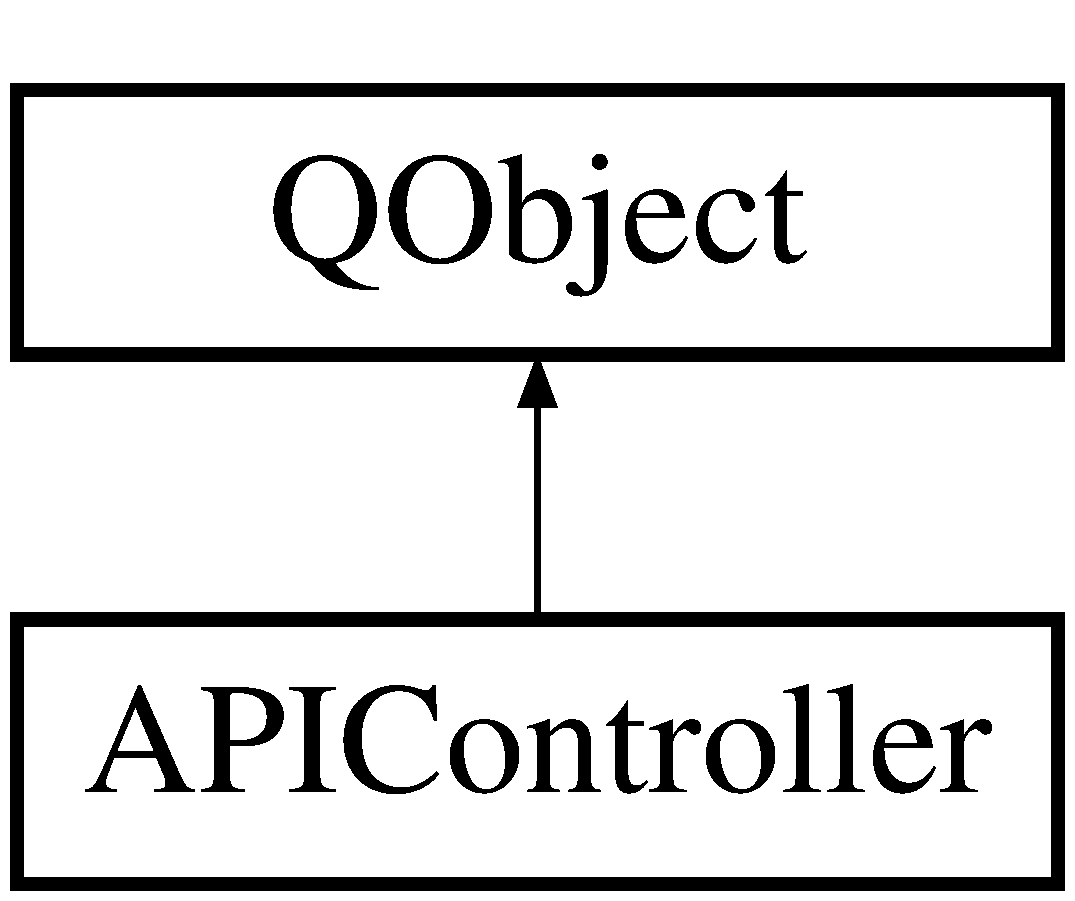
\includegraphics[height=2.000000cm]{class_a_p_i_controller}
\end{center}
\end{figure}
\subsection*{Public Slots}
\begin{DoxyCompactItemize}
\item 
void \hyperlink{class_a_p_i_controller_ac1fe4dd7b8df2e4cceb554e46bea894d}{handle\+Config\+Url} (const \hyperlink{class_a_p_i_request}{A\+P\+I\+Request} \&request, \hyperlink{class_a_p_i_response}{A\+P\+I\+Response} $\ast$response)
\item 
void \hyperlink{class_a_p_i_controller_a6274380cb71807d07d813b7e67e0c0c2}{handle\+Module\+Config\+Url} (const \hyperlink{class_a_p_i_request}{A\+P\+I\+Request} \&request, \hyperlink{class_a_p_i_response}{A\+P\+I\+Response} $\ast$response)
\item 
void \hyperlink{class_a_p_i_controller_a3d32a4cf1f6a06697b09d43a2be140cf}{handle\+Device\+Config\+Url} (const \hyperlink{class_a_p_i_request}{A\+P\+I\+Request} \&request, \hyperlink{class_a_p_i_response}{A\+P\+I\+Response} $\ast$response)
\item 
void \hyperlink{class_a_p_i_controller_a3217b84dcc811d83e4c7241a5e19c35c}{handle\+Get\+Notification\+List\+Url} (const \hyperlink{class_a_p_i_request}{A\+P\+I\+Request} \&request, \hyperlink{class_a_p_i_response}{A\+P\+I\+Response} $\ast$response)
\item 
void \hyperlink{class_a_p_i_controller_afb480d438e18a2551229810280a65806}{handle\+Download\+Firmware\+Url} (const \hyperlink{class_a_p_i_request}{A\+P\+I\+Request} \&request, \hyperlink{class_a_p_i_response}{A\+P\+I\+Response} $\ast$response)
\item 
void \hyperlink{class_a_p_i_controller_ad37a3ecaf99e3b7c43ecb4ec4873fea9}{handle\+Get\+Controller\+List} (const \hyperlink{class_a_p_i_request}{A\+P\+I\+Request} \&request, \hyperlink{class_a_p_i_response}{A\+P\+I\+Response} $\ast$response)
\item 
void \hyperlink{class_a_p_i_controller_a20ce823aeb786d2af26fde41c2dc74a1}{handle\+Get\+Controller\+Module\+List} (const \hyperlink{class_a_p_i_request}{A\+P\+I\+Request} \&request, \hyperlink{class_a_p_i_response}{A\+P\+I\+Response} $\ast$response)
\item 
void \hyperlink{class_a_p_i_controller_a0e01eab749423dcfff0b595abf4175ad}{handle\+Controller\+Reset} (const \hyperlink{class_a_p_i_request}{A\+P\+I\+Request} \&request, \hyperlink{class_a_p_i_response}{A\+P\+I\+Response} $\ast$response)
\item 
void \hyperlink{class_a_p_i_controller_a0d4deeaff703bb7d60eb344e6ee9f8cb}{handle\+Controller\+Reset\+Config} (const \hyperlink{class_a_p_i_request}{A\+P\+I\+Request} \&request, \hyperlink{class_a_p_i_response}{A\+P\+I\+Response} $\ast$response)
\item 
void \hyperlink{class_a_p_i_controller_a9b2f08f4b0a67c0a4f6891a9d8601b93}{handle\+Reset\+Notification\+List} (const \hyperlink{class_a_p_i_request}{A\+P\+I\+Request} \&request, \hyperlink{class_a_p_i_response}{A\+P\+I\+Response} $\ast$response)
\end{DoxyCompactItemize}
\subsection*{Public Member Functions}
\begin{DoxyCompactItemize}
\item 
\hyperlink{class_a_p_i_controller_a779b634bce4b7fcbec9fca8f5f8f63e6}{A\+P\+I\+Controller} (Q\+Object $\ast$parent=nullptr)
\end{DoxyCompactItemize}


\subsection{Detailed Description}
A\+PI handler class for a L\+CS controller. This class handles all A\+PI requests for a controller. Two types of requests are made as it relates to a L\+CS controller; \char`\"{}/\+A\+P\+I/...\char`\"{} requests sent from an external source like a web page or an application and a \char`\"{}/controller/...\char`\"{} requests sent by a L\+CS controller to download information from the application server. 

\hyperlink{class_a_p_i_controller}{A\+P\+I\+Controller} 

\subsection{Constructor \& Destructor Documentation}
\mbox{\Hypertarget{class_a_p_i_controller_a779b634bce4b7fcbec9fca8f5f8f63e6}\label{class_a_p_i_controller_a779b634bce4b7fcbec9fca8f5f8f63e6}} 
\index{A\+P\+I\+Controller@{A\+P\+I\+Controller}!A\+P\+I\+Controller@{A\+P\+I\+Controller}}
\index{A\+P\+I\+Controller@{A\+P\+I\+Controller}!A\+P\+I\+Controller@{A\+P\+I\+Controller}}
\subsubsection{\texorpdfstring{A\+P\+I\+Controller()}{APIController()}}
{\footnotesize\ttfamily A\+P\+I\+Controller\+::\+A\+P\+I\+Controller (\begin{DoxyParamCaption}\item[{Q\+Object $\ast$}]{parent = {\ttfamily nullptr} }\end{DoxyParamCaption})\hspace{0.3cm}{\ttfamily [explicit]}}

Contstructor Creates a controller A\+PI handler. The constructor registers a \hyperlink{class_url_handler}{Url Handler} object for the following url\textquotesingle{}s\+: \char`\"{}/controller/config\char`\"{} Download the controller\textquotesingle{}s configuration. \char`\"{}/controller/module/config\char`\"{} Download a controller module\textquotesingle{}s configuration. \char`\"{}/controller/device/config\char`\"{} Download a device\textquotesingle{}s configuration. \char`\"{}/controller/notification\+\_\+list\char`\"{} Download a controller\textquotesingle{}s list of \char`\"{}\+Controllers to Notify\char`\"{}. 

\subsection{Member Function Documentation}
\mbox{\Hypertarget{class_a_p_i_controller_ac1fe4dd7b8df2e4cceb554e46bea894d}\label{class_a_p_i_controller_ac1fe4dd7b8df2e4cceb554e46bea894d}} 
\index{A\+P\+I\+Controller@{A\+P\+I\+Controller}!handle\+Config\+Url@{handle\+Config\+Url}}
\index{handle\+Config\+Url@{handle\+Config\+Url}!A\+P\+I\+Controller@{A\+P\+I\+Controller}}
\subsubsection{\texorpdfstring{handle\+Config\+Url}{handleConfigUrl}}
{\footnotesize\ttfamily void A\+P\+I\+Controller\+::handle\+Config\+Url (\begin{DoxyParamCaption}\item[{const \hyperlink{class_a_p_i_request}{A\+P\+I\+Request} \&}]{request,  }\item[{\hyperlink{class_a_p_i_response}{A\+P\+I\+Response} $\ast$}]{response }\end{DoxyParamCaption})\hspace{0.3cm}{\ttfamily [slot]}}

A\+PI \char`\"{}/controller/config\char`\"{} Downloads a controller\textquotesingle{}s configuration 
\begin{DoxyParams}{Parameters}
{\em request} & \hyperlink{class_a_p_i_request}{A\+P\+I\+Request} containing the url of the request including the serial number of the controller. \\
\hline
{\em response} & \hyperlink{class_a_p_i_response}{A\+P\+I\+Response} with the payload set to the controller\textquotesingle{}s configuration information in J\+S\+ON format. \\
\hline
\end{DoxyParams}
\mbox{\Hypertarget{class_a_p_i_controller_a0e01eab749423dcfff0b595abf4175ad}\label{class_a_p_i_controller_a0e01eab749423dcfff0b595abf4175ad}} 
\index{A\+P\+I\+Controller@{A\+P\+I\+Controller}!handle\+Controller\+Reset@{handle\+Controller\+Reset}}
\index{handle\+Controller\+Reset@{handle\+Controller\+Reset}!A\+P\+I\+Controller@{A\+P\+I\+Controller}}
\subsubsection{\texorpdfstring{handle\+Controller\+Reset}{handleControllerReset}}
{\footnotesize\ttfamily void A\+P\+I\+Controller\+::handle\+Controller\+Reset (\begin{DoxyParamCaption}\item[{const \hyperlink{class_a_p_i_request}{A\+P\+I\+Request} \&}]{request,  }\item[{\hyperlink{class_a_p_i_response}{A\+P\+I\+Response} $\ast$}]{response }\end{DoxyParamCaption})\hspace{0.3cm}{\ttfamily [slot]}}

A\+PI \char`\"{}/api/send\+\_\+controller\+\_\+reset\char`\"{} Sends a S\+Y\+S\+\_\+\+R\+E\+B\+O\+O\+T\+\_\+\+C\+O\+N\+T\+R\+O\+L\+L\+ER broadcast U\+DP message instructing the controller(s) to restart. 
\begin{DoxyParams}{Parameters}
{\em request} & \hyperlink{class_a_p_i_request}{A\+P\+I\+Request} containing the url of the request including the controller\textquotesingle{}s serial number. If the serial number is less than 1, all controllers are restarted. \\
\hline
{\em response} & \hyperlink{class_a_p_i_response}{A\+P\+I\+Response} unused. \\
\hline
\end{DoxyParams}
\mbox{\Hypertarget{class_a_p_i_controller_a0d4deeaff703bb7d60eb344e6ee9f8cb}\label{class_a_p_i_controller_a0d4deeaff703bb7d60eb344e6ee9f8cb}} 
\index{A\+P\+I\+Controller@{A\+P\+I\+Controller}!handle\+Controller\+Reset\+Config@{handle\+Controller\+Reset\+Config}}
\index{handle\+Controller\+Reset\+Config@{handle\+Controller\+Reset\+Config}!A\+P\+I\+Controller@{A\+P\+I\+Controller}}
\subsubsection{\texorpdfstring{handle\+Controller\+Reset\+Config}{handleControllerResetConfig}}
{\footnotesize\ttfamily void A\+P\+I\+Controller\+::handle\+Controller\+Reset\+Config (\begin{DoxyParamCaption}\item[{const \hyperlink{class_a_p_i_request}{A\+P\+I\+Request} \&}]{request,  }\item[{\hyperlink{class_a_p_i_response}{A\+P\+I\+Response} $\ast$}]{response }\end{DoxyParamCaption})\hspace{0.3cm}{\ttfamily [slot]}}

A\+PI \char`\"{}/api/send\+\_\+controller\+\_\+reset\+\_\+config\char`\"{} Sends a S\+Y\+S\+\_\+\+R\+E\+S\+E\+T\+\_\+\+C\+O\+N\+F\+IG broadcast U\+DP message instructing the controller(s) to delete all configuration data. 
\begin{DoxyParams}{Parameters}
{\em request} & \hyperlink{class_a_p_i_request}{A\+P\+I\+Request} containing the url of the request including the controller\textquotesingle{}s serial number. If the serial number is less than 1, all controllers delete their configuration data. \\
\hline
{\em response} & \hyperlink{class_a_p_i_response}{A\+P\+I\+Response} unused. \\
\hline
\end{DoxyParams}
\mbox{\Hypertarget{class_a_p_i_controller_a3d32a4cf1f6a06697b09d43a2be140cf}\label{class_a_p_i_controller_a3d32a4cf1f6a06697b09d43a2be140cf}} 
\index{A\+P\+I\+Controller@{A\+P\+I\+Controller}!handle\+Device\+Config\+Url@{handle\+Device\+Config\+Url}}
\index{handle\+Device\+Config\+Url@{handle\+Device\+Config\+Url}!A\+P\+I\+Controller@{A\+P\+I\+Controller}}
\subsubsection{\texorpdfstring{handle\+Device\+Config\+Url}{handleDeviceConfigUrl}}
{\footnotesize\ttfamily void A\+P\+I\+Controller\+::handle\+Device\+Config\+Url (\begin{DoxyParamCaption}\item[{const \hyperlink{class_a_p_i_request}{A\+P\+I\+Request} \&}]{request,  }\item[{\hyperlink{class_a_p_i_response}{A\+P\+I\+Response} $\ast$}]{response }\end{DoxyParamCaption})\hspace{0.3cm}{\ttfamily [slot]}}

A\+PI \char`\"{}/controller/device/config\char`\"{} Downloads a device\textquotesingle{}s configuration 
\begin{DoxyParams}{Parameters}
{\em request} & \hyperlink{class_a_p_i_request}{A\+P\+I\+Request} containing the url of the request including the device\+ID. \\
\hline
{\em response} & \hyperlink{class_a_p_i_response}{A\+P\+I\+Response} with the payload set to the device\textquotesingle{}s configuration information in J\+S\+ON format. \\
\hline
\end{DoxyParams}
\mbox{\Hypertarget{class_a_p_i_controller_afb480d438e18a2551229810280a65806}\label{class_a_p_i_controller_afb480d438e18a2551229810280a65806}} 
\index{A\+P\+I\+Controller@{A\+P\+I\+Controller}!handle\+Download\+Firmware\+Url@{handle\+Download\+Firmware\+Url}}
\index{handle\+Download\+Firmware\+Url@{handle\+Download\+Firmware\+Url}!A\+P\+I\+Controller@{A\+P\+I\+Controller}}
\subsubsection{\texorpdfstring{handle\+Download\+Firmware\+Url}{handleDownloadFirmwareUrl}}
{\footnotesize\ttfamily void A\+P\+I\+Controller\+::handle\+Download\+Firmware\+Url (\begin{DoxyParamCaption}\item[{const \hyperlink{class_a_p_i_request}{A\+P\+I\+Request} \&}]{request,  }\item[{\hyperlink{class_a_p_i_response}{A\+P\+I\+Response} $\ast$}]{response }\end{DoxyParamCaption})\hspace{0.3cm}{\ttfamily [slot]}}

A\+PI \char`\"{}/controller/firmware\char`\"{} Downloads a controller\textquotesingle{}s firmware. 
\begin{DoxyParams}{Parameters}
{\em request} & \hyperlink{class_a_p_i_request}{A\+P\+I\+Request} containing the url of the request including the controller\textquotesingle{}s serial number. \\
\hline
{\em response} & \hyperlink{class_a_p_i_response}{A\+P\+I\+Response} not used. \\
\hline
\end{DoxyParams}
\mbox{\Hypertarget{class_a_p_i_controller_ad37a3ecaf99e3b7c43ecb4ec4873fea9}\label{class_a_p_i_controller_ad37a3ecaf99e3b7c43ecb4ec4873fea9}} 
\index{A\+P\+I\+Controller@{A\+P\+I\+Controller}!handle\+Get\+Controller\+List@{handle\+Get\+Controller\+List}}
\index{handle\+Get\+Controller\+List@{handle\+Get\+Controller\+List}!A\+P\+I\+Controller@{A\+P\+I\+Controller}}
\subsubsection{\texorpdfstring{handle\+Get\+Controller\+List}{handleGetControllerList}}
{\footnotesize\ttfamily void A\+P\+I\+Controller\+::handle\+Get\+Controller\+List (\begin{DoxyParamCaption}\item[{const \hyperlink{class_a_p_i_request}{A\+P\+I\+Request} \&}]{request,  }\item[{\hyperlink{class_a_p_i_response}{A\+P\+I\+Response} $\ast$}]{response }\end{DoxyParamCaption})\hspace{0.3cm}{\ttfamily [slot]}}

A\+PI \char`\"{}/api/controller\+\_\+list\char`\"{} Downloads a list of all controllers. 
\begin{DoxyParams}{Parameters}
{\em request} & \hyperlink{class_a_p_i_request}{A\+P\+I\+Request} containing the url of the request including the controller\textquotesingle{}s serial number. \\
\hline
{\em response} & \hyperlink{class_a_p_i_response}{A\+P\+I\+Response} with the payload set to the list of controllers in J\+S\+ON format. \\
\hline
\end{DoxyParams}
\mbox{\Hypertarget{class_a_p_i_controller_a20ce823aeb786d2af26fde41c2dc74a1}\label{class_a_p_i_controller_a20ce823aeb786d2af26fde41c2dc74a1}} 
\index{A\+P\+I\+Controller@{A\+P\+I\+Controller}!handle\+Get\+Controller\+Module\+List@{handle\+Get\+Controller\+Module\+List}}
\index{handle\+Get\+Controller\+Module\+List@{handle\+Get\+Controller\+Module\+List}!A\+P\+I\+Controller@{A\+P\+I\+Controller}}
\subsubsection{\texorpdfstring{handle\+Get\+Controller\+Module\+List}{handleGetControllerModuleList}}
{\footnotesize\ttfamily void A\+P\+I\+Controller\+::handle\+Get\+Controller\+Module\+List (\begin{DoxyParamCaption}\item[{const \hyperlink{class_a_p_i_request}{A\+P\+I\+Request} \&}]{request,  }\item[{\hyperlink{class_a_p_i_response}{A\+P\+I\+Response} $\ast$}]{response }\end{DoxyParamCaption})\hspace{0.3cm}{\ttfamily [slot]}}

A\+PI \char`\"{}/api/controller\+\_\+module\+\_\+list\char`\"{} Downloads a list of modules for a controller or a specific module. 
\begin{DoxyParams}{Parameters}
{\em request} & \hyperlink{class_a_p_i_request}{A\+P\+I\+Request} containing the url of the request including the controller\textquotesingle{}s ID or a specific module ID. \\
\hline
{\em response} & \hyperlink{class_a_p_i_response}{A\+P\+I\+Response} with the payload set to the list of controller modules in J\+S\+ON format. \\
\hline
\end{DoxyParams}
\mbox{\Hypertarget{class_a_p_i_controller_a3217b84dcc811d83e4c7241a5e19c35c}\label{class_a_p_i_controller_a3217b84dcc811d83e4c7241a5e19c35c}} 
\index{A\+P\+I\+Controller@{A\+P\+I\+Controller}!handle\+Get\+Notification\+List\+Url@{handle\+Get\+Notification\+List\+Url}}
\index{handle\+Get\+Notification\+List\+Url@{handle\+Get\+Notification\+List\+Url}!A\+P\+I\+Controller@{A\+P\+I\+Controller}}
\subsubsection{\texorpdfstring{handle\+Get\+Notification\+List\+Url}{handleGetNotificationListUrl}}
{\footnotesize\ttfamily void A\+P\+I\+Controller\+::handle\+Get\+Notification\+List\+Url (\begin{DoxyParamCaption}\item[{const \hyperlink{class_a_p_i_request}{A\+P\+I\+Request} \&}]{request,  }\item[{\hyperlink{class_a_p_i_response}{A\+P\+I\+Response} $\ast$}]{response }\end{DoxyParamCaption})\hspace{0.3cm}{\ttfamily [slot]}}

A\+PI \char`\"{}/controller/notification\+\_\+list\char`\"{} Downloads a controller\textquotesingle{}s controllers-\/to-\/notify list. 
\begin{DoxyParams}{Parameters}
{\em request} & \hyperlink{class_a_p_i_request}{A\+P\+I\+Request} containing the url of the request including the controller\textquotesingle{}s serial number. \\
\hline
{\em response} & \hyperlink{class_a_p_i_response}{A\+P\+I\+Response} with the payload set to the controller\textquotesingle{}s list of controllers-\/to-\/notify in J\+S\+ON format. \\
\hline
\end{DoxyParams}
\mbox{\Hypertarget{class_a_p_i_controller_a6274380cb71807d07d813b7e67e0c0c2}\label{class_a_p_i_controller_a6274380cb71807d07d813b7e67e0c0c2}} 
\index{A\+P\+I\+Controller@{A\+P\+I\+Controller}!handle\+Module\+Config\+Url@{handle\+Module\+Config\+Url}}
\index{handle\+Module\+Config\+Url@{handle\+Module\+Config\+Url}!A\+P\+I\+Controller@{A\+P\+I\+Controller}}
\subsubsection{\texorpdfstring{handle\+Module\+Config\+Url}{handleModuleConfigUrl}}
{\footnotesize\ttfamily void A\+P\+I\+Controller\+::handle\+Module\+Config\+Url (\begin{DoxyParamCaption}\item[{const \hyperlink{class_a_p_i_request}{A\+P\+I\+Request} \&}]{request,  }\item[{\hyperlink{class_a_p_i_response}{A\+P\+I\+Response} $\ast$}]{response }\end{DoxyParamCaption})\hspace{0.3cm}{\ttfamily [slot]}}

A\+PI \char`\"{}/controller/module/config\char`\"{} Downloads a controller module\textquotesingle{}s configuration 
\begin{DoxyParams}{Parameters}
{\em request} & \hyperlink{class_a_p_i_request}{A\+P\+I\+Request} containing the url of the request including the serial number of the controller and the address of the module. \\
\hline
{\em response} & \hyperlink{class_a_p_i_response}{A\+P\+I\+Response} with the payload set to the controller module\textquotesingle{}s configuration information in J\+S\+ON format. \\
\hline
\end{DoxyParams}
\mbox{\Hypertarget{class_a_p_i_controller_a9b2f08f4b0a67c0a4f6891a9d8601b93}\label{class_a_p_i_controller_a9b2f08f4b0a67c0a4f6891a9d8601b93}} 
\index{A\+P\+I\+Controller@{A\+P\+I\+Controller}!handle\+Reset\+Notification\+List@{handle\+Reset\+Notification\+List}}
\index{handle\+Reset\+Notification\+List@{handle\+Reset\+Notification\+List}!A\+P\+I\+Controller@{A\+P\+I\+Controller}}
\subsubsection{\texorpdfstring{handle\+Reset\+Notification\+List}{handleResetNotificationList}}
{\footnotesize\ttfamily void A\+P\+I\+Controller\+::handle\+Reset\+Notification\+List (\begin{DoxyParamCaption}\item[{const \hyperlink{class_a_p_i_request}{A\+P\+I\+Request} \&}]{request,  }\item[{\hyperlink{class_a_p_i_response}{A\+P\+I\+Response} $\ast$}]{response }\end{DoxyParamCaption})\hspace{0.3cm}{\ttfamily [slot]}}

A\+PI \char`\"{}/api/send\+\_\+controller\+\_\+reset\+\_\+notification\+\_\+list\char`\"{} Sends a S\+Y\+S\+\_\+\+R\+E\+S\+E\+T\+\_\+\+N\+O\+T\+I\+F\+I\+C\+A\+T\+I\+O\+N\+\_\+\+L\+I\+ST broadcast U\+DP message instructing the controller(s) to delete controllers-\/to-\/notify list. The controller responds by sending a /controller/notification\+\_\+list to the application server. 
\begin{DoxyParams}{Parameters}
{\em request} & \hyperlink{class_a_p_i_request}{A\+P\+I\+Request} containing the url of the request including the controller\textquotesingle{}s serial number. If the serial number is less than 1, all controllers delete their controllers-\/to-\/notify list. \\
\hline
{\em response} & \hyperlink{class_a_p_i_response}{A\+P\+I\+Response} unused. \\
\hline
\end{DoxyParams}


The documentation for this class was generated from the following files\+:\begin{DoxyCompactItemize}
\item 
L\+C\+S\+Server/A\+P\+I\+Controller.\+h\item 
L\+C\+S\+Server/A\+P\+I\+Controller.\+cpp\end{DoxyCompactItemize}

\hypertarget{class_a_p_i_device}{}\section{A\+P\+I\+Device Class Reference}
\label{class_a_p_i_device}\index{A\+P\+I\+Device@{A\+P\+I\+Device}}


A\+PI handler class for a L\+CS device.  




{\ttfamily \#include $<$A\+P\+I\+Device.\+h$>$}

Inheritance diagram for A\+P\+I\+Device\+:\begin{figure}[H]
\begin{center}
\leavevmode
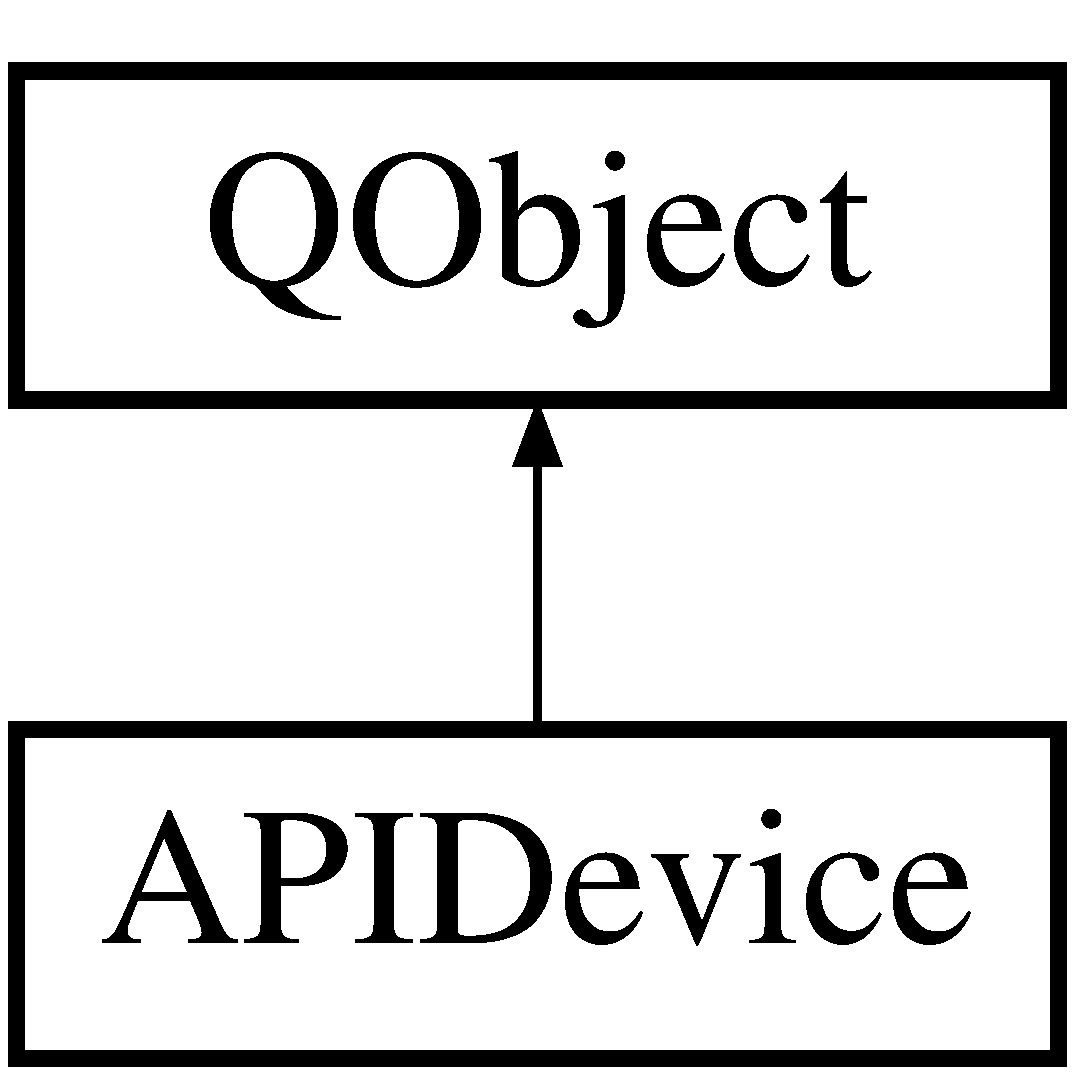
\includegraphics[height=2.000000cm]{class_a_p_i_device}
\end{center}
\end{figure}
\subsection*{Public Slots}
\begin{DoxyCompactItemize}
\item 
void \hyperlink{class_a_p_i_device_a1e74a10d605557654fe5be02a9db87ab}{handle\+Get\+Device\+List} (const \hyperlink{class_a_p_i_request}{A\+P\+I\+Request} \&request, \hyperlink{class_a_p_i_response}{A\+P\+I\+Response} $\ast$response)
\item 
void \hyperlink{class_a_p_i_device_a5be87488af611d8ef61501a07e4a39d9}{handle\+Get\+Device\+Property\+List} (const \hyperlink{class_a_p_i_request}{A\+P\+I\+Request} \&request, \hyperlink{class_a_p_i_response}{A\+P\+I\+Response} $\ast$response)
\item 
void \hyperlink{class_a_p_i_device_ad5a4f48e5cf4767426fd179446501c53}{handle\+Get\+Module\+Device\+Port\+List} (const \hyperlink{class_a_p_i_request}{A\+P\+I\+Request} \&request, \hyperlink{class_a_p_i_response}{A\+P\+I\+Response} $\ast$response)
\item 
void \hyperlink{class_a_p_i_device_a794458df71d6f24a8b8dccbbdf9235da}{handle\+Send\+Device\+Config} (const \hyperlink{class_a_p_i_request}{A\+P\+I\+Request} \&request, \hyperlink{class_a_p_i_response}{A\+P\+I\+Response} $\ast$response)
\item 
void \hyperlink{class_a_p_i_device_aabc5cc49832ebe6779cf70c1b38ad4c9}{handle\+Create\+Device} (const \hyperlink{class_a_p_i_request}{A\+P\+I\+Request} \&request, \hyperlink{class_a_p_i_response}{A\+P\+I\+Response} $\ast$response)
\item 
void \hyperlink{class_a_p_i_device_a9fa95a9f88e738477ed5e32e22ae6990}{handle\+Lock\+Device} (const \hyperlink{class_a_p_i_request}{A\+P\+I\+Request} \&request, \hyperlink{class_a_p_i_response}{A\+P\+I\+Response} $\ast$response)
\item 
void \hyperlink{class_a_p_i_device_a4424a0e2b44177c7b3af3b9fd9aca875}{on\+Device\+Status\+Changed} (int device\+ID, int status, bool locked)
\end{DoxyCompactItemize}
\subsection*{Signals}
\begin{DoxyCompactItemize}
\item 
\mbox{\Hypertarget{class_a_p_i_device_a1096381146a1c545b194d4bb63b32b8b}\label{class_a_p_i_device_a1096381146a1c545b194d4bb63b32b8b}} 
void \hyperlink{class_a_p_i_device_a1096381146a1c545b194d4bb63b32b8b}{send\+Notification\+Message} (const Q\+String \&url, const Q\+Json\+Object \&obj)
\begin{DoxyCompactList}\small\item\em Notifies interested parties that a device\textquotesingle{}s status or lock state has changed. \end{DoxyCompactList}\end{DoxyCompactItemize}
\subsection*{Public Member Functions}
\begin{DoxyCompactItemize}
\item 
\hyperlink{class_a_p_i_device_ab983034826edbff2b4246002b22081a5}{A\+P\+I\+Device} (Q\+Object $\ast$parent=nullptr)
\end{DoxyCompactItemize}


\subsection{Detailed Description}
A\+PI handler class for a L\+CS device. 

\{get\} /api/device\+\_\+list\+:serial\+Number,module\+ID,controller\+ID,class\+Code,device\+ID Get a list of devices  Get\+Device\+List  Device

\{Number\} \mbox{[}serial\+Number\mbox{]} filter device list by a specific controller\textquotesingle{}s serial number.  \{Number\}\mbox{[}module\+ID\mbox{]} filter device list by a specific controller module\textquotesingle{}s ID.  \{Number\} \mbox{[}controller\+ID\mbox{]} filter device list by a specific controller\textquotesingle{}s ID.  \{Number\} \mbox{[}class\+Code\mbox{]} filter device list by a specific device classification.  \{Number\} \mbox{[}device\+ID\mbox{]} filter device list by a specific device ID.  Returns a list of devices. If no parameters are supplied, all devices are returned.  \{Number\} device\+Class Device classification.  \{String\} device\+Description Device\textquotesingle{}s description.  \{Number\} device\+ID Device\textquotesingle{}s ID.  \{String\} device\+Name Device\textquotesingle{}s name  \{Number\} device\+State Device\textquotesingle{}s current state.  Example usage\+: \href{http://localhost:8080/api/device_list?controllerID=30}{\tt http\+://localhost\+:8080/api/device\+\_\+list?controller\+I\+D=30}  \{json\} Success-\/\+Response\+: H\+T\+T\+P/1.\+1 200 OK \mbox{[}\{ \char`\"{}device\+Class\char`\"{}\+: \char`\"{}5\char`\"{}, \char`\"{}device\+Description\char`\"{}\+: \char`\"{}\char`\"{}, \char`\"{}device\+I\+D\char`\"{}\+: \char`\"{}19\char`\"{}, \char`\"{}device\+Name\char`\"{}\+: \char`\"{}\+G\+K Mine Signal\char`\"{}, \char`\"{}device\+State\char`\"{}\+: 0, \} \mbox{]}  \{get\} /api/device\+\_\+property\+\_\+list\+:device\+ID Get device\+Property entries for a given device  Get\+Device\+Property\+List  Device

\{Number\} device\+ID device\textquotesingle{}s ID.  Returns a list of device\+Property entries for a given device..  \{Number\} device\+ID Device\textquotesingle{}s ID.  \{Number\} id device\+Property\textquotesingle{}s id.  \{Number\} key Device Property key.  \{Number\} value Device Property value.  Example usage\+: \href{http://localhost:8080/api/device_property_list?deviceID=1}{\tt http\+://localhost\+:8080/api/device\+\_\+property\+\_\+list?device\+I\+D=1}  \{json\} Success-\/\+Response\+: H\+T\+T\+P/1.\+1 200 OK \mbox{[}\{ \char`\"{}device\+I\+D\char`\"{}\+: \char`\"{}1\char`\"{}, \char`\"{}id\char`\"{}\+: \char`\"{}243\char`\"{}, \char`\"{}key\char`\"{}\+: \char`\"{}\+M\+O\+T\+O\+R\+P\+I\+N\char`\"{}, \char`\"{}value\char`\"{}\+: \char`\"{}1\char`\"{} \}, \{ \char`\"{}device\+I\+D\char`\"{}\+: \char`\"{}1\char`\"{}, \char`\"{}id\char`\"{}\+: \char`\"{}244\char`\"{}, \char`\"{}key\char`\"{}\+: \char`\"{}\+I\+N\+P\+U\+T\+P\+I\+N\char`\"{}, \char`\"{}value\char`\"{}\+: \char`\"{}1\char`\"{} \} \mbox{]}  \{get\} /api/module\+\_\+device\+\_\+port\+\_\+list\+:device\+ID,module\+ID Get module/port entries for a given device  Get\+Module\+Device\+Port\+List  Device

\{Number\} \mbox{[}device\+ID\} device\textquotesingle{}s ID.  \{Number\} \mbox{[}modle\+ID\mbox{]} controller\+Module\textquotesingle{}s ID.  Returns a list of module\+Device\+Port entries for a given device or module. This table cross-\/references a device to one or more modules. This allows a single device entry to be used with multiple modules; useful for Panel\+Input\+Device and Panel\+Output\+Device, etc.  \{Number\} id module\+Device\+Port\textquotesingle{}s ID.  \{Number\} device\+ID device\textquotesingle{}s ID.  \{Number\} controller\+Module\+ID controller\+Module\textquotesingle{}s id.  \{String\} module\+Name controller\+Module\textquotesingle{}s name.  \{Number\} module\+Class controller\+Module\textquotesingle{}s class.  \{String\} device\+Name device\textquotesingle{}s name.  \{Number\} device\+Class device\textquotesingle{}s class.  \{Number\} port port the device is connected to.  Example usage\+: \href{http://localhost:8080/api/device_property_list?deviceID=11}{\tt http\+://localhost\+:8080/api/device\+\_\+property\+\_\+list?device\+I\+D=11}  \{json\} Success-\/\+Response\+: H\+T\+T\+P/1.\+1 200 OK \mbox{[}\{ \char`\"{}controller\+Module\+I\+D\char`\"{}\+: \char`\"{}13\char`\"{}, \char`\"{}device\+Class\char`\"{}\+: \char`\"{}6\char`\"{}, \char`\"{}device\+I\+D\char`\"{}\+: \char`\"{}11\char`\"{}, \char`\"{}device\+Name\char`\"{}\+: \char`\"{}\+Block 30-\/1\char`\"{}, \char`\"{}id\char`\"{}\+: \char`\"{}1\char`\"{}, \char`\"{}module\+Class\char`\"{}\+: \char`\"{}8\char`\"{}, \char`\"{}module\+Name\char`\"{}\+: \char`\"{}\+Blocks 30-\/1, 30-\/9, 31-\/1, 31-\/9\char`\"{}, \char`\"{}port\char`\"{}\+: \char`\"{}7\char`\"{} \} \mbox{]}  \{get\} /api/send\+\_\+device\+\_\+config\+:device\+ID Reset device\textquotesingle{}s configuration  Device\+Config\+Reset  Device

\{Number\} \mbox{[}device\+ID\mbox{]} The device\textquotesingle{}s id. If 0 or excluded, all devices will reset their configuration data.  Sends a S\+Y\+S\+\_\+\+R\+E\+S\+E\+T\+\_\+\+D\+E\+V\+I\+C\+E\+\_\+\+C\+O\+N\+F\+IG broadcast U\+DP message instructing the device(s) to re-\/download its configuration data.  Example usage\+: \href{http://localhost:8080/api/send_device_config?deviceID=1}{\tt http\+://localhost\+:8080/api/send\+\_\+device\+\_\+config?device\+I\+D=1}  \{post\} /api/create\+\_\+device\+:create\+Extra Create a device entry  Create\+Device  Device

\{Number\} \mbox{[}create\+Extra\mbox{]} Flag that, when set to true, instructs the system to create additional companion devices.  Creates a new device entry. In addition to the device table entry, any required device\+Property entries are also created. If the create\+Extra flag is set to 1, additional devices are created. For turnouts, two Panel\+Output devices are created for the red and green panel L\+E\+Ds. For a block device, one Panel\+Output device is created for the yellow L\+ED.  \{Number\} controller\+Module\+ID Controller Module\textquotesingle{}s ID to which the device is connected.  \{Number\} device\+Class Device\textquotesingle{}s classification populated with the supplied device\+Class.  \{String\} device\+Description Device\textquotesingle{}s description.  \{String\} device\+Name Device Device\textquotesingle{}s name.  \{Number\} id Device\textquotesingle{}s new ID.  \{Number\} port/pin Port to which the device is connected.  This example creates a new Turnout device entry. In addition to the device table entry, two entries are also added to the device\+Property table; M\+O\+T\+O\+R\+P\+IN and I\+N\+P\+U\+T\+P\+IN with values set to 0\+: \href{http://localhost:8080/api/create_device?createExtra=1}{\tt http\+://localhost\+:8080/api/create\+\_\+device?create\+Extra=1} body\+: \{ \char`\"{}device\+Name\char`\"{}\+: \char`\"{}\+T\+Y-\/\+N\+E\+W\char`\"{}, \char`\"{}device\+Description\char`\"{}\+: \char`\"{}\+Description\char`\"{}, \char`\"{}device\+Class\char`\"{}\+: \char`\"{}1\char`\"{} \}  \{json\} Success-\/\+Response\+: H\+T\+T\+P/1.\+1 200 OK \mbox{[}\{ \char`\"{}controller\+Module\+I\+D\char`\"{}\+: \char`\"{}0\char`\"{}, \char`\"{}device\+Class\char`\"{}\+: \char`\"{}1\char`\"{}, \char`\"{}device\+Description\char`\"{}\+: \char`\"{}\char`\"{}, \char`\"{}device\+Name\char`\"{}\+: \char`\"{}\char`\"{}, \char`\"{}id\char`\"{}\+: \char`\"{}83\char`\"{}, \char`\"{}port\char`\"{}\+: \char`\"{}0\char`\"{} \} \mbox{]}  \{get\} /api/notification/device Device Status Change  Device\+Status\+Change\+Notification  A\+P\+I\+Notifications  off

Notification message sent when a device\textquotesingle{}s state changes.  \{String\} url Notification url.  \{Number\} device\+ID Device\textquotesingle{}s ID.  \{Number\} device\+State Device\textquotesingle{}s new state  \{Number=0,1\} locked Device\textquotesingle{}s locked state. 0 = unlocked, 1 = locked.  \{json\} Success-\/\+Response\+: \{ \char`\"{}url\char`\"{}\+: \char`\"{}/api/notification/device\char`\"{}, \char`\"{}device\+I\+D\char`\"{}\+: \char`\"{}1\char`\"{}, \char`\"{}device\+State\char`\"{}\+: \char`\"{}2\char`\"{}, \char`\"{}locked\char`\"{}\+: \char`\"{}0\char`\"{} \}\hyperlink{class_a_p_i_device}{A\+P\+I\+Device} This class handles basic A\+PI requests for a device. \hyperlink{class_a_p_i_signal}{A\+P\+I\+Signal}, \hyperlink{class_a_p_i_turnout}{A\+P\+I\+Turnout} and \hyperlink{class_a_p_i_route}{A\+P\+I\+Route} handle device-\/specific requests. 

\subsection{Constructor \& Destructor Documentation}
\mbox{\Hypertarget{class_a_p_i_device_ab983034826edbff2b4246002b22081a5}\label{class_a_p_i_device_ab983034826edbff2b4246002b22081a5}} 
\index{A\+P\+I\+Device@{A\+P\+I\+Device}!A\+P\+I\+Device@{A\+P\+I\+Device}}
\index{A\+P\+I\+Device@{A\+P\+I\+Device}!A\+P\+I\+Device@{A\+P\+I\+Device}}
\subsubsection{\texorpdfstring{A\+P\+I\+Device()}{APIDevice()}}
{\footnotesize\ttfamily A\+P\+I\+Device\+::\+A\+P\+I\+Device (\begin{DoxyParamCaption}\item[{Q\+Object $\ast$}]{parent = {\ttfamily nullptr} }\end{DoxyParamCaption})\hspace{0.3cm}{\ttfamily [explicit]}}

Contstructor Creates a device A\+PI handler. The constructor registers a \hyperlink{class_url_handler}{Url Handler} objects. See the A\+PI documentation for information on the U\+RL\textquotesingle{}s handled by this class. 

\subsection{Member Function Documentation}
\mbox{\Hypertarget{class_a_p_i_device_aabc5cc49832ebe6779cf70c1b38ad4c9}\label{class_a_p_i_device_aabc5cc49832ebe6779cf70c1b38ad4c9}} 
\index{A\+P\+I\+Device@{A\+P\+I\+Device}!handle\+Create\+Device@{handle\+Create\+Device}}
\index{handle\+Create\+Device@{handle\+Create\+Device}!A\+P\+I\+Device@{A\+P\+I\+Device}}
\subsubsection{\texorpdfstring{handle\+Create\+Device}{handleCreateDevice}}
{\footnotesize\ttfamily void A\+P\+I\+Device\+::handle\+Create\+Device (\begin{DoxyParamCaption}\item[{const \hyperlink{class_a_p_i_request}{A\+P\+I\+Request} \&}]{request,  }\item[{\hyperlink{class_a_p_i_response}{A\+P\+I\+Response} $\ast$}]{response }\end{DoxyParamCaption})\hspace{0.3cm}{\ttfamily [slot]}}

A\+PI \char`\"{}/api/create\+\_\+device\char`\"{} Creates a new device entry. device\+Property entries (if applicable) are also created for the supplied device\+Class. 
\begin{DoxyParams}{Parameters}
{\em request} & \hyperlink{class_a_p_i_request}{A\+P\+I\+Request} containing the url of the request including the device\textquotesingle{}s class. \\
\hline
{\em response} & \hyperlink{class_a_p_i_response}{A\+P\+I\+Response} with the payload set to the new device data in J\+S\+ON format. \\
\hline
\end{DoxyParams}
\mbox{\Hypertarget{class_a_p_i_device_a1e74a10d605557654fe5be02a9db87ab}\label{class_a_p_i_device_a1e74a10d605557654fe5be02a9db87ab}} 
\index{A\+P\+I\+Device@{A\+P\+I\+Device}!handle\+Get\+Device\+List@{handle\+Get\+Device\+List}}
\index{handle\+Get\+Device\+List@{handle\+Get\+Device\+List}!A\+P\+I\+Device@{A\+P\+I\+Device}}
\subsubsection{\texorpdfstring{handle\+Get\+Device\+List}{handleGetDeviceList}}
{\footnotesize\ttfamily void A\+P\+I\+Device\+::handle\+Get\+Device\+List (\begin{DoxyParamCaption}\item[{const \hyperlink{class_a_p_i_request}{A\+P\+I\+Request} \&}]{request,  }\item[{\hyperlink{class_a_p_i_response}{A\+P\+I\+Response} $\ast$}]{response }\end{DoxyParamCaption})\hspace{0.3cm}{\ttfamily [slot]}}

A\+PI \char`\"{}/api/device\+\_\+list\char`\"{} Downloads a list of all devices. 
\begin{DoxyParams}{Parameters}
{\em request} & \hyperlink{class_a_p_i_request}{A\+P\+I\+Request} containing the url of the request including any filtering parameters. \\
\hline
{\em response} & \hyperlink{class_a_p_i_response}{A\+P\+I\+Response} with the payload set to the list of devices in J\+S\+ON format. \\
\hline
\end{DoxyParams}
\mbox{\Hypertarget{class_a_p_i_device_a5be87488af611d8ef61501a07e4a39d9}\label{class_a_p_i_device_a5be87488af611d8ef61501a07e4a39d9}} 
\index{A\+P\+I\+Device@{A\+P\+I\+Device}!handle\+Get\+Device\+Property\+List@{handle\+Get\+Device\+Property\+List}}
\index{handle\+Get\+Device\+Property\+List@{handle\+Get\+Device\+Property\+List}!A\+P\+I\+Device@{A\+P\+I\+Device}}
\subsubsection{\texorpdfstring{handle\+Get\+Device\+Property\+List}{handleGetDevicePropertyList}}
{\footnotesize\ttfamily void A\+P\+I\+Device\+::handle\+Get\+Device\+Property\+List (\begin{DoxyParamCaption}\item[{const \hyperlink{class_a_p_i_request}{A\+P\+I\+Request} \&}]{request,  }\item[{\hyperlink{class_a_p_i_response}{A\+P\+I\+Response} $\ast$}]{response }\end{DoxyParamCaption})\hspace{0.3cm}{\ttfamily [slot]}}

A\+PI \char`\"{}/api/device\+\_\+property\+\_\+list\char`\"{} Downloads a list of device\+Property entries for a given device\+ID. 
\begin{DoxyParams}{Parameters}
{\em request} & \hyperlink{class_a_p_i_request}{A\+P\+I\+Request} containing the url of the request including the device\textquotesingle{}s ID. \\
\hline
{\em response} & \hyperlink{class_a_p_i_response}{A\+P\+I\+Response} with the payload set to the list of device\+Properties in J\+S\+ON format. \\
\hline
\end{DoxyParams}
\mbox{\Hypertarget{class_a_p_i_device_ad5a4f48e5cf4767426fd179446501c53}\label{class_a_p_i_device_ad5a4f48e5cf4767426fd179446501c53}} 
\index{A\+P\+I\+Device@{A\+P\+I\+Device}!handle\+Get\+Module\+Device\+Port\+List@{handle\+Get\+Module\+Device\+Port\+List}}
\index{handle\+Get\+Module\+Device\+Port\+List@{handle\+Get\+Module\+Device\+Port\+List}!A\+P\+I\+Device@{A\+P\+I\+Device}}
\subsubsection{\texorpdfstring{handle\+Get\+Module\+Device\+Port\+List}{handleGetModuleDevicePortList}}
{\footnotesize\ttfamily void A\+P\+I\+Device\+::handle\+Get\+Module\+Device\+Port\+List (\begin{DoxyParamCaption}\item[{const \hyperlink{class_a_p_i_request}{A\+P\+I\+Request} \&}]{request,  }\item[{\hyperlink{class_a_p_i_response}{A\+P\+I\+Response} $\ast$}]{response }\end{DoxyParamCaption})\hspace{0.3cm}{\ttfamily [slot]}}

A\+PI \char`\"{}/api/module\+\_\+device\+\_\+port\+\_\+list\char`\"{} Downloads a list of module/port entries for a given device\+ID. 
\begin{DoxyParams}{Parameters}
{\em request} & \hyperlink{class_a_p_i_request}{A\+P\+I\+Request} containing the url of the request including the device\textquotesingle{}s ID. \\
\hline
{\em response} & \hyperlink{class_a_p_i_response}{A\+P\+I\+Response} with the payload set to the list of device\+Properties in J\+S\+ON format. \\
\hline
\end{DoxyParams}
\mbox{\Hypertarget{class_a_p_i_device_a9fa95a9f88e738477ed5e32e22ae6990}\label{class_a_p_i_device_a9fa95a9f88e738477ed5e32e22ae6990}} 
\index{A\+P\+I\+Device@{A\+P\+I\+Device}!handle\+Lock\+Device@{handle\+Lock\+Device}}
\index{handle\+Lock\+Device@{handle\+Lock\+Device}!A\+P\+I\+Device@{A\+P\+I\+Device}}
\subsubsection{\texorpdfstring{handle\+Lock\+Device}{handleLockDevice}}
{\footnotesize\ttfamily void A\+P\+I\+Device\+::handle\+Lock\+Device (\begin{DoxyParamCaption}\item[{const \hyperlink{class_a_p_i_request}{A\+P\+I\+Request} \&}]{request,  }\item[{\hyperlink{class_a_p_i_response}{A\+P\+I\+Response} $\ast$}]{response }\end{DoxyParamCaption})\hspace{0.3cm}{\ttfamily [slot]}}

A\+PI \char`\"{}/api/lock\+\_\+device\char`\"{} Sends a S\+Y\+S\+\_\+\+L\+O\+C\+K\+\_\+\+D\+E\+V\+I\+CE broadcast U\+DP message instructing the device to lock/unlock. 
\begin{DoxyParams}{Parameters}
{\em request} & \hyperlink{class_a_p_i_request}{A\+P\+I\+Request} containing the url of the request including the device\textquotesingle{}s ID and the lock flag. \\
\hline
{\em response} & \hyperlink{class_a_p_i_response}{A\+P\+I\+Response} unused. \\
\hline
\end{DoxyParams}
\mbox{\Hypertarget{class_a_p_i_device_a794458df71d6f24a8b8dccbbdf9235da}\label{class_a_p_i_device_a794458df71d6f24a8b8dccbbdf9235da}} 
\index{A\+P\+I\+Device@{A\+P\+I\+Device}!handle\+Send\+Device\+Config@{handle\+Send\+Device\+Config}}
\index{handle\+Send\+Device\+Config@{handle\+Send\+Device\+Config}!A\+P\+I\+Device@{A\+P\+I\+Device}}
\subsubsection{\texorpdfstring{handle\+Send\+Device\+Config}{handleSendDeviceConfig}}
{\footnotesize\ttfamily void A\+P\+I\+Device\+::handle\+Send\+Device\+Config (\begin{DoxyParamCaption}\item[{const \hyperlink{class_a_p_i_request}{A\+P\+I\+Request} \&}]{request,  }\item[{\hyperlink{class_a_p_i_response}{A\+P\+I\+Response} $\ast$}]{response }\end{DoxyParamCaption})\hspace{0.3cm}{\ttfamily [slot]}}

A\+PI \char`\"{}/api/send\+\_\+device\+\_\+config\char`\"{} Sends a S\+Y\+S\+\_\+\+R\+E\+S\+E\+T\+\_\+\+D\+E\+V\+I\+C\+E\+\_\+\+C\+O\+N\+F\+IG broadcast U\+DP message instructing the device to reset its configuration. 
\begin{DoxyParams}{Parameters}
{\em request} & \hyperlink{class_a_p_i_request}{A\+P\+I\+Request} containing the url of the request including the device\textquotesingle{}s ID. \\
\hline
{\em response} & \hyperlink{class_a_p_i_response}{A\+P\+I\+Response} unused. \\
\hline
\end{DoxyParams}
\mbox{\Hypertarget{class_a_p_i_device_a4424a0e2b44177c7b3af3b9fd9aca875}\label{class_a_p_i_device_a4424a0e2b44177c7b3af3b9fd9aca875}} 
\index{A\+P\+I\+Device@{A\+P\+I\+Device}!on\+Device\+Status\+Changed@{on\+Device\+Status\+Changed}}
\index{on\+Device\+Status\+Changed@{on\+Device\+Status\+Changed}!A\+P\+I\+Device@{A\+P\+I\+Device}}
\subsubsection{\texorpdfstring{on\+Device\+Status\+Changed}{onDeviceStatusChanged}}
{\footnotesize\ttfamily void A\+P\+I\+Device\+::on\+Device\+Status\+Changed (\begin{DoxyParamCaption}\item[{int}]{device\+ID,  }\item[{int}]{status,  }\item[{bool}]{locked }\end{DoxyParamCaption})\hspace{0.3cm}{\ttfamily [slot]}}

Monitors the \hyperlink{class_device_manager}{Device\+Manager} for device status changes 
\begin{DoxyParams}{Parameters}
{\em device\+ID} & int Device ID of the device. \\
\hline
{\em status} & int The device\textquotesingle{}s new status. \\
\hline
{\em locked} & int The device\textquotesingle{}s new locked state. \\
\hline
\end{DoxyParams}


The documentation for this class was generated from the following files\+:\begin{DoxyCompactItemize}
\item 
L\+C\+S\+Server/A\+P\+I\+Device.\+h\item 
L\+C\+S\+Server/A\+P\+I\+Device.\+cpp\end{DoxyCompactItemize}

\hypertarget{class_a_p_i_entity}{}\section{A\+P\+I\+Entity Class Reference}
\label{class_a_p_i_entity}\index{A\+P\+I\+Entity@{A\+P\+I\+Entity}}


A\+PI handler class for L\+CS database entities. This class handles basic database fetch and C\+R\+UD operations (Create, Update and Delete). See the A\+PI documentation for more information.  




{\ttfamily \#include $<$A\+P\+I\+Entity.\+h$>$}

Inheritance diagram for A\+P\+I\+Entity\+:\begin{figure}[H]
\begin{center}
\leavevmode
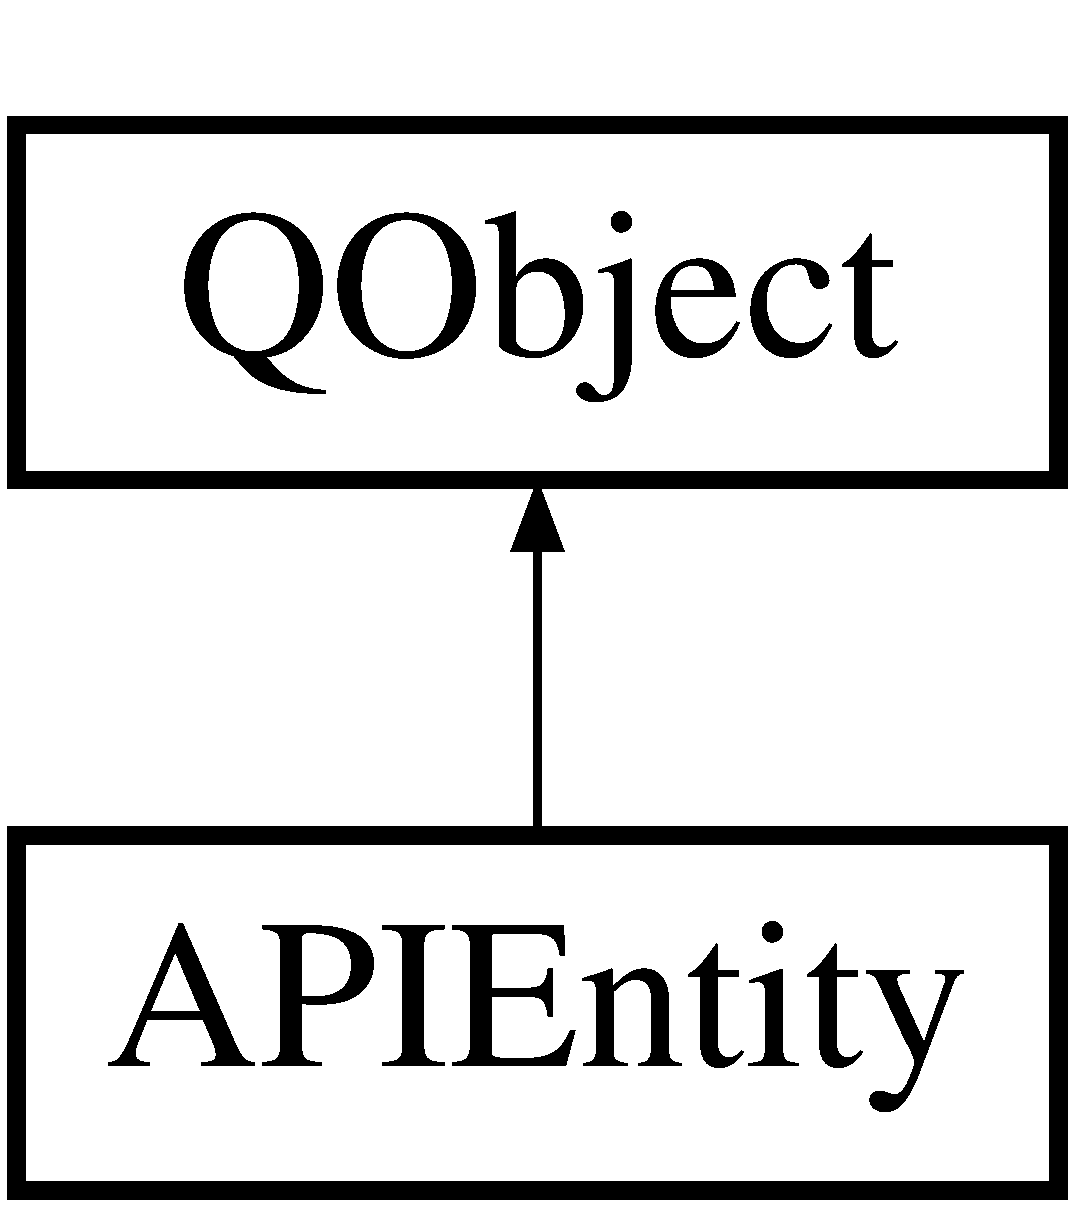
\includegraphics[height=2.000000cm]{class_a_p_i_entity}
\end{center}
\end{figure}
\subsection*{Public Member Functions}
\begin{DoxyCompactItemize}
\item 
\mbox{\Hypertarget{class_a_p_i_entity_a1408a64bcc760d3add4f9d5d67903e96}\label{class_a_p_i_entity_a1408a64bcc760d3add4f9d5d67903e96}} 
\hyperlink{class_a_p_i_entity_a1408a64bcc760d3add4f9d5d67903e96}{A\+P\+I\+Entity} (Q\+Object $\ast$parent=nullptr)
\begin{DoxyCompactList}\small\item\em Contstructor. \end{DoxyCompactList}\item 
void \hyperlink{class_a_p_i_entity_a66ea6b2523afbb3acebaadf3aea1ec6c}{handle\+Client} (const \hyperlink{class_a_p_i_request}{A\+P\+I\+Request} \&request, \hyperlink{class_a_p_i_response}{A\+P\+I\+Response} $\ast$response)
\item 
Q\+Byte\+Array \hyperlink{class_a_p_i_entity_a4ff9b9128b1ad595dd07006544c99dee}{fetch\+Entity} (const Q\+String \&name, const Q\+Url \&url)
\item 
Q\+Byte\+Array \hyperlink{class_a_p_i_entity_a5f2de518701f362000bb6eb341fbf95b}{save\+Entity} (const Q\+String \&name, const Q\+String \&json\+Text)
\item 
Q\+Byte\+Array \hyperlink{class_a_p_i_entity_a8bbe43bbc389472d7a7fd9e8a2283c82}{add\+Entity} (const Q\+String \&name, const Q\+String \&json\+Text)
\item 
void \hyperlink{class_a_p_i_entity_ade40ac225523f1d00ed7c1eb8bdfec96}{delete\+Entity} (const Q\+String \&name, const Q\+String \&json\+Text)
\end{DoxyCompactItemize}


\subsection{Detailed Description}
A\+PI handler class for L\+CS database entities. This class handles basic database fetch and C\+R\+UD operations (Create, Update and Delete). See the A\+PI documentation for more information. 

\{get\} /api/entity/\mbox{[}Entity\+Name\mbox{]}\+:where Fetch  Fetch\+Entity  Entity

\{String\} field\+Name (optional) Any combination of Field\+Name=value pairs can be passed to filter the list returned. Multiple field/value pairs are joined as an \char`\"{}\+A\+N\+D\char`\"{} in the generated W\+H\+E\+RE clause.  Fetches records from the \mbox{[}Entity\+Name\mbox{]} table with the optional filters applied.  This example fetches all controller\+Modules with an address of 2\+: \href{http://localhost:8080/api/entity/controllerModule?address=2}{\tt http\+://localhost\+:8080/api/entity/controller\+Module?address=2}  \{json\} Success-\/\+Response\+: H\+T\+T\+P/1.\+1 200 OK \mbox{[}\{ \char`\"{}address\char`\"{}\+: \char`\"{}2\char`\"{}, \char`\"{}controller\+I\+D\char`\"{}\+: \char`\"{}24\char`\"{}, \char`\"{}disable\char`\"{}\+: \char`\"{}0\char`\"{}, \char`\"{}id\char`\"{}\+: \char`\"{}6\char`\"{}, \char`\"{}module\+Class\char`\"{}\+: \char`\"{}1\char`\"{}, \char`\"{}module\+Name\char`\"{}\+: \char`\"{}\+T\+Y30-\/4\char`\"{} \}, \{ \char`\"{}address\char`\"{}\+: \char`\"{}2\char`\"{}, \char`\"{}controller\+I\+D\char`\"{}\+: \char`\"{}31\char`\"{}, \char`\"{}disable\char`\"{}\+: \char`\"{}0\char`\"{}, \char`\"{}id\char`\"{}\+: \char`\"{}18\char`\"{}, \char`\"{}module\+Class\char`\"{}\+: \char`\"{}9\char`\"{}, \char`\"{}module\+Name\char`\"{}\+: \char`\"{}\+C\+A Panel1 Output 2\char`\"{} \}, \{ \char`\"{}address\char`\"{}\+: \char`\"{}2\char`\"{}, \char`\"{}controller\+I\+D\char`\"{}\+: \char`\"{}34\char`\"{}, \char`\"{}disable\char`\"{}\+: \char`\"{}0\char`\"{}, \char`\"{}id\char`\"{}\+: \char`\"{}23\char`\"{}, \char`\"{}module\+Class\char`\"{}\+: \char`\"{}9\char`\"{}, \char`\"{}module\+Name\char`\"{}\+: \char`\"{}\+C\+A Aux Panel Output 2\char`\"{} \} \mbox{]}  \{put\} /api/entity/\mbox{[}Entity\+Name\mbox{]} Update an Entity  Update\+Entity  Entity

Updates a specific record in the \mbox{[}Entity\+Name\mbox{]} table. The entity is sent as a J\+S\+ON document.  This example updates a \char`\"{}route\char`\"{} with an ID of 7. Note\+: You only need to supply the fields that are modified, however like this example, you may include all fields. \+: \href{http://localhost:8080/api/entity/route}{\tt http\+://localhost\+:8080/api/entity/route} \begin{DoxyVerb}body:
{
  "id": 7,
  "routeName": "CA 1"
  "routeDescription": "New Description"
}\end{DoxyVerb}


\{post\} /api/entity/\mbox{[}Entity\+Name\mbox{]} Add a new Entity  Add\+Entity  Entity

Adds a new record into the \mbox{[}Entity\+Name\mbox{]} table. The entity is sent as a J\+S\+ON document.  This example adds a new \char`\"{}route\char`\"{}. Note\+: Exclude the ID field as this field will be auto-\/generated. The newly generated id is part of the returned J\+S\+ON payload. \+: \href{http://localhost:8080/api/entity/route}{\tt http\+://localhost\+:8080/api/entity/route} \begin{DoxyVerb}body:
{
  "routeName": "New Route"
  "routeDescription": "New Route Description"
}
\end{DoxyVerb}


\{json\} Success-\/\+Response\+: H\+T\+T\+P/1.\+1 200 OK \mbox{[}\{ \char`\"{}id\char`\"{}\+: \char`\"{}15\char`\"{}, \char`\"{}route\+Description\char`\"{}\+: \char`\"{}\+New Route\char`\"{}, \char`\"{}route\+Name\char`\"{}\+: \char`\"{}\+New Route Description\char`\"{} \} \mbox{]}  \{delete\} /api/entity/\mbox{[}Entity\+Name\mbox{]} Delete an Entity  Delete\+Entity  Entity

Deletes a specific record in the \mbox{[}Entity\+Name\mbox{]} table. The entity is sent as a J\+S\+ON document.  This example deletes a \char`\"{}route\char`\"{} with an ID of 7.\+: \href{http://localhost:8080/api/entity/route}{\tt http\+://localhost\+:8080/api/entity/route} \begin{DoxyVerb}body:
{
  "id": 7,
}\end{DoxyVerb}
 \hyperlink{class_a_p_i_entity}{A\+P\+I\+Entity} 

\subsection{Member Function Documentation}
\mbox{\Hypertarget{class_a_p_i_entity_a8bbe43bbc389472d7a7fd9e8a2283c82}\label{class_a_p_i_entity_a8bbe43bbc389472d7a7fd9e8a2283c82}} 
\index{A\+P\+I\+Entity@{A\+P\+I\+Entity}!add\+Entity@{add\+Entity}}
\index{add\+Entity@{add\+Entity}!A\+P\+I\+Entity@{A\+P\+I\+Entity}}
\subsubsection{\texorpdfstring{add\+Entity()}{addEntity()}}
{\footnotesize\ttfamily Q\+Byte\+Array A\+P\+I\+Entity\+::add\+Entity (\begin{DoxyParamCaption}\item[{const Q\+String \&}]{name,  }\item[{const Q\+String \&}]{json\+Text }\end{DoxyParamCaption})}

Adds a new row into the \mbox{[}name\mbox{]} table in the database. 
\begin{DoxyParams}{Parameters}
{\em name} & Q\+String containing the table name. \\
\hline
{\em json\+Text} & Q\+String containing the data to be added. \\
\hline
\end{DoxyParams}
\mbox{\Hypertarget{class_a_p_i_entity_ade40ac225523f1d00ed7c1eb8bdfec96}\label{class_a_p_i_entity_ade40ac225523f1d00ed7c1eb8bdfec96}} 
\index{A\+P\+I\+Entity@{A\+P\+I\+Entity}!delete\+Entity@{delete\+Entity}}
\index{delete\+Entity@{delete\+Entity}!A\+P\+I\+Entity@{A\+P\+I\+Entity}}
\subsubsection{\texorpdfstring{delete\+Entity()}{deleteEntity()}}
{\footnotesize\ttfamily void A\+P\+I\+Entity\+::delete\+Entity (\begin{DoxyParamCaption}\item[{const Q\+String \&}]{name,  }\item[{const Q\+String \&}]{json\+Text }\end{DoxyParamCaption})}

Deletes a specific row in the \mbox{[}name\mbox{]} table in the database. 
\begin{DoxyParams}{Parameters}
{\em name} & Q\+String containing the table name. \\
\hline
{\em json\+Text} & Q\+String containing key data for the row to be deleted. \\
\hline
\end{DoxyParams}
\mbox{\Hypertarget{class_a_p_i_entity_a4ff9b9128b1ad595dd07006544c99dee}\label{class_a_p_i_entity_a4ff9b9128b1ad595dd07006544c99dee}} 
\index{A\+P\+I\+Entity@{A\+P\+I\+Entity}!fetch\+Entity@{fetch\+Entity}}
\index{fetch\+Entity@{fetch\+Entity}!A\+P\+I\+Entity@{A\+P\+I\+Entity}}
\subsubsection{\texorpdfstring{fetch\+Entity()}{fetchEntity()}}
{\footnotesize\ttfamily Q\+Byte\+Array A\+P\+I\+Entity\+::fetch\+Entity (\begin{DoxyParamCaption}\item[{const Q\+String \&}]{name,  }\item[{const Q\+Url \&}]{url }\end{DoxyParamCaption})}

Fetches an entity list from the database with optional where clause values. 
\begin{DoxyParams}{Parameters}
{\em name} & Q\+String containing the table name from which data is fetched. \\
\hline
{\em url} & Q\+Url containing optional field/value pairs used in the W\+H\+E\+RE clause. \\
\hline
\end{DoxyParams}
\mbox{\Hypertarget{class_a_p_i_entity_a66ea6b2523afbb3acebaadf3aea1ec6c}\label{class_a_p_i_entity_a66ea6b2523afbb3acebaadf3aea1ec6c}} 
\index{A\+P\+I\+Entity@{A\+P\+I\+Entity}!handle\+Client@{handle\+Client}}
\index{handle\+Client@{handle\+Client}!A\+P\+I\+Entity@{A\+P\+I\+Entity}}
\subsubsection{\texorpdfstring{handle\+Client()}{handleClient()}}
{\footnotesize\ttfamily void A\+P\+I\+Entity\+::handle\+Client (\begin{DoxyParamCaption}\item[{const \hyperlink{class_a_p_i_request}{A\+P\+I\+Request} \&}]{request,  }\item[{\hyperlink{class_a_p_i_response}{A\+P\+I\+Response} $\ast$}]{response }\end{DoxyParamCaption})}

A\+PI \char`\"{}/api/entity/\mbox{[}\+Entity\+Name\mbox{]}\char`\"{} Handles fetch, add, update and delete functions on a database table. \mbox{[}Entity\+Name\mbox{]} represents the target table. 
\begin{DoxyParams}{Parameters}
{\em request} & \hyperlink{class_a_p_i_request}{A\+P\+I\+Request} containing the url of the request. Used by the fetch (get) operation as optional where clause entries. \\
\hline
{\em response} & \hyperlink{class_a_p_i_response}{A\+P\+I\+Response} with the payload set to the data returned from the database. \\
\hline
\end{DoxyParams}
\mbox{\Hypertarget{class_a_p_i_entity_a5f2de518701f362000bb6eb341fbf95b}\label{class_a_p_i_entity_a5f2de518701f362000bb6eb341fbf95b}} 
\index{A\+P\+I\+Entity@{A\+P\+I\+Entity}!save\+Entity@{save\+Entity}}
\index{save\+Entity@{save\+Entity}!A\+P\+I\+Entity@{A\+P\+I\+Entity}}
\subsubsection{\texorpdfstring{save\+Entity()}{saveEntity()}}
{\footnotesize\ttfamily Q\+Byte\+Array A\+P\+I\+Entity\+::save\+Entity (\begin{DoxyParamCaption}\item[{const Q\+String \&}]{name,  }\item[{const Q\+String \&}]{json\+Text }\end{DoxyParamCaption})}

Updates a specific row in the \mbox{[}name\mbox{]} table in the database. 
\begin{DoxyParams}{Parameters}
{\em name} & Q\+String containing the table name. \\
\hline
{\em json\+Text} & Q\+String containing the data to be updated. \\
\hline
\end{DoxyParams}


The documentation for this class was generated from the following files\+:\begin{DoxyCompactItemize}
\item 
L\+C\+S\+Server/A\+P\+I\+Entity.\+h\item 
L\+C\+S\+Server/A\+P\+I\+Entity.\+cpp\end{DoxyCompactItemize}

\hypertarget{class_a_p_i_request}{}\section{A\+P\+I\+Request Class Reference}
\label{class_a_p_i_request}\index{A\+P\+I\+Request@{A\+P\+I\+Request}}


Contains information for an A\+PI web request.  




{\ttfamily \#include $<$A\+P\+I\+Request.\+h$>$}

\subsection*{Public Member Functions}
\begin{DoxyCompactItemize}
\item 
\mbox{\Hypertarget{class_a_p_i_request_aa1b6f8f309547967edbfc2f6636df3a4}\label{class_a_p_i_request_aa1b6f8f309547967edbfc2f6636df3a4}} 
\hyperlink{class_a_p_i_request_aa1b6f8f309547967edbfc2f6636df3a4}{A\+P\+I\+Request} (void)
\begin{DoxyCompactList}\small\item\em Contstructor. \end{DoxyCompactList}\item 
\hyperlink{class_a_p_i_request_a5c6b7f4e52cf0d36bd3bb2280ab59331}{A\+P\+I\+Request} (Net\+Action\+Type action\+Type, const Q\+Url url)
\item 
\mbox{\Hypertarget{class_a_p_i_request_a0b237561a193b67440be9787117f90d1}\label{class_a_p_i_request_a0b237561a193b67440be9787117f90d1}} 
\hyperlink{class_a_p_i_request_a0b237561a193b67440be9787117f90d1}{A\+P\+I\+Request} (const \hyperlink{class_a_p_i_request}{A\+P\+I\+Request} \&other)
\begin{DoxyCompactList}\small\item\em Copy Contstructor. \end{DoxyCompactList}\item 
\mbox{\Hypertarget{class_a_p_i_request_ae2d4cf9cce8e40de3158b681d4402551}\label{class_a_p_i_request_ae2d4cf9cce8e40de3158b681d4402551}} 
Net\+Action\+Type \hyperlink{class_a_p_i_request_ae2d4cf9cce8e40de3158b681d4402551}{get\+Net\+Action\+Type} (void) const
\begin{DoxyCompactList}\small\item\em Returns the H\+T\+TP action type. \end{DoxyCompactList}\item 
\mbox{\Hypertarget{class_a_p_i_request_ab4f5dc1d54250fc927872cfcc59cc3cc}\label{class_a_p_i_request_ab4f5dc1d54250fc927872cfcc59cc3cc}} 
Q\+Url \hyperlink{class_a_p_i_request_ab4f5dc1d54250fc927872cfcc59cc3cc}{get\+Url} (void) const
\begin{DoxyCompactList}\small\item\em Returns the requesting U\+RL. \end{DoxyCompactList}\item 
\mbox{\Hypertarget{class_a_p_i_request_af70046cd59021cc3877f380ca46ac6e7}\label{class_a_p_i_request_af70046cd59021cc3877f380ca46ac6e7}} 
Q\+Byte\+Array \hyperlink{class_a_p_i_request_af70046cd59021cc3877f380ca46ac6e7}{get\+Payload} (void) const
\begin{DoxyCompactList}\small\item\em Access function for a message payload. Usually a J\+S\+ON document. \end{DoxyCompactList}\item 
\mbox{\Hypertarget{class_a_p_i_request_a2d16b4ff383297fff242db0b71139c2b}\label{class_a_p_i_request_a2d16b4ff383297fff242db0b71139c2b}} 
void \hyperlink{class_a_p_i_request_a2d16b4ff383297fff242db0b71139c2b}{set\+Payload} (const Q\+Byte\+Array \&value)
\begin{DoxyCompactList}\small\item\em Sets the message payload. \end{DoxyCompactList}\item 
\mbox{\Hypertarget{class_a_p_i_request_a5e07ea518a0bb0a750ec8f2d58e9acc5}\label{class_a_p_i_request_a5e07ea518a0bb0a750ec8f2d58e9acc5}} 
\hyperlink{class_a_p_i_request}{A\+P\+I\+Request} \& \hyperlink{class_a_p_i_request_a5e07ea518a0bb0a750ec8f2d58e9acc5}{operator=} (const \hyperlink{class_a_p_i_request}{A\+P\+I\+Request} \&other)
\begin{DoxyCompactList}\small\item\em Assignment operator. \end{DoxyCompactList}\end{DoxyCompactItemize}


\subsection{Detailed Description}
Contains information for an A\+PI web request. 

\hyperlink{class_a_p_i_request}{A\+P\+I\+Request} This class contains all information as it relates to a R\+E\+ST A\+PI web request. 

\subsection{Constructor \& Destructor Documentation}
\mbox{\Hypertarget{class_a_p_i_request_a5c6b7f4e52cf0d36bd3bb2280ab59331}\label{class_a_p_i_request_a5c6b7f4e52cf0d36bd3bb2280ab59331}} 
\index{A\+P\+I\+Request@{A\+P\+I\+Request}!A\+P\+I\+Request@{A\+P\+I\+Request}}
\index{A\+P\+I\+Request@{A\+P\+I\+Request}!A\+P\+I\+Request@{A\+P\+I\+Request}}
\subsubsection{\texorpdfstring{A\+P\+I\+Request()}{APIRequest()}}
{\footnotesize\ttfamily A\+P\+I\+Request\+::\+A\+P\+I\+Request (\begin{DoxyParamCaption}\item[{Net\+Action\+Type}]{action\+Type,  }\item[{const Q\+Url}]{url }\end{DoxyParamCaption})}

Contstructor 
\begin{DoxyParams}{Parameters}
{\em Net\+Action\+Type} & H\+T\+TP action type  Q\+Url Full url of the request including parameters \\
\hline
\end{DoxyParams}


The documentation for this class was generated from the following files\+:\begin{DoxyCompactItemize}
\item 
L\+C\+S\+Server/A\+P\+I\+Request.\+h\item 
L\+C\+S\+Server/A\+P\+I\+Request.\+cpp\end{DoxyCompactItemize}

\hypertarget{class_a_p_i_response}{}\section{A\+P\+I\+Response Class Reference}
\label{class_a_p_i_response}\index{A\+P\+I\+Response@{A\+P\+I\+Response}}
\subsection*{Public Member Functions}
\begin{DoxyCompactItemize}
\item 
\mbox{\Hypertarget{class_a_p_i_response_ad9f5238fb178a139f7d90f0024c094bd}\label{class_a_p_i_response_ad9f5238fb178a139f7d90f0024c094bd}} 
{\bfseries A\+P\+I\+Response} (const \hyperlink{class_a_p_i_response}{A\+P\+I\+Response} \&other)
\item 
\mbox{\Hypertarget{class_a_p_i_response_a0ac0de9b5ec19f313d1571936d88c2f1}\label{class_a_p_i_response_a0ac0de9b5ec19f313d1571936d88c2f1}} 
Q\+String {\bfseries get\+Return\+Code} (void) const
\item 
\mbox{\Hypertarget{class_a_p_i_response_a4c749e490345ac4d497678d2272dd5f0}\label{class_a_p_i_response_a4c749e490345ac4d497678d2272dd5f0}} 
void {\bfseries set\+Return\+Code} (const Q\+String \&value)
\item 
\mbox{\Hypertarget{class_a_p_i_response_a6861e22ef4409885114aac404760daeb}\label{class_a_p_i_response_a6861e22ef4409885114aac404760daeb}} 
Q\+String {\bfseries get\+Content\+Type} (void) const
\item 
\mbox{\Hypertarget{class_a_p_i_response_a67c8ba2ac3155ae8472f453a36f469f5}\label{class_a_p_i_response_a67c8ba2ac3155ae8472f453a36f469f5}} 
void {\bfseries set\+Contenet\+Type} (const Q\+String \&value)
\item 
\mbox{\Hypertarget{class_a_p_i_response_ae58db2525b25db3b244a71c8d10b6b98}\label{class_a_p_i_response_ae58db2525b25db3b244a71c8d10b6b98}} 
Q\+Byte\+Array {\bfseries get\+Payload} (void) const
\item 
\mbox{\Hypertarget{class_a_p_i_response_a7b36f0565b798ad4740f83b58488f079}\label{class_a_p_i_response_a7b36f0565b798ad4740f83b58488f079}} 
void {\bfseries set\+Payload} (const Q\+Byte\+Array \&value)
\item 
\mbox{\Hypertarget{class_a_p_i_response_a6c757d09db4b79b845b4ecc699c87905}\label{class_a_p_i_response_a6c757d09db4b79b845b4ecc699c87905}} 
\hyperlink{class_a_p_i_response}{A\+P\+I\+Response} \& {\bfseries operator=} (const \hyperlink{class_a_p_i_response}{A\+P\+I\+Response} \&other)
\end{DoxyCompactItemize}


The documentation for this class was generated from the following files\+:\begin{DoxyCompactItemize}
\item 
L\+C\+S\+Server/A\+P\+I\+Response.\+h\item 
L\+C\+S\+Server/A\+P\+I\+Response.\+cpp\end{DoxyCompactItemize}

\hypertarget{class_a_p_i_route}{}\section{A\+P\+I\+Route Class Reference}
\label{class_a_p_i_route}\index{A\+P\+I\+Route@{A\+P\+I\+Route}}


{\ttfamily \#include $<$A\+P\+I\+Route.\+h$>$}

Inheritance diagram for A\+P\+I\+Route\+:\begin{figure}[H]
\begin{center}
\leavevmode
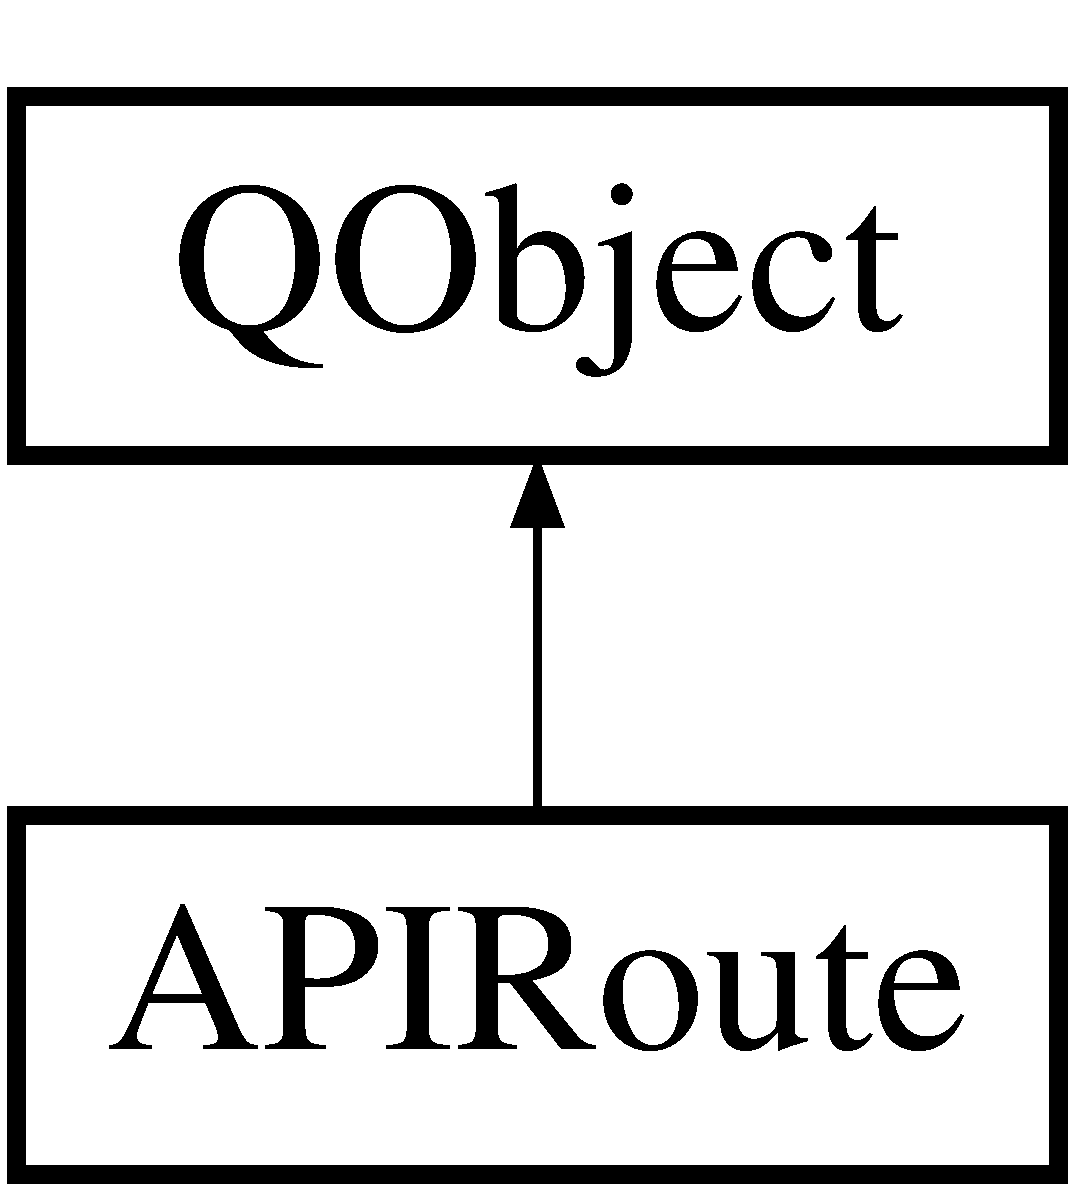
\includegraphics[height=2.000000cm]{class_a_p_i_route}
\end{center}
\end{figure}
\subsection*{Public Slots}
\begin{DoxyCompactItemize}
\item 
\mbox{\Hypertarget{class_a_p_i_route_a23f1b30a95e806760968daf23e2b3fa1}\label{class_a_p_i_route_a23f1b30a95e806760968daf23e2b3fa1}} 
void {\bfseries handle\+Activate\+Route\+Url} (const \hyperlink{class_a_p_i_request}{A\+P\+I\+Request} \&request, \hyperlink{class_a_p_i_response}{A\+P\+I\+Response} $\ast$response)
\item 
\mbox{\Hypertarget{class_a_p_i_route_a2edf94cf41f8fba5b1ed5f5eca217968}\label{class_a_p_i_route_a2edf94cf41f8fba5b1ed5f5eca217968}} 
void {\bfseries handle\+Lock\+Route\+Url} (const \hyperlink{class_a_p_i_request}{A\+P\+I\+Request} \&request, \hyperlink{class_a_p_i_response}{A\+P\+I\+Response} $\ast$response)
\item 
\mbox{\Hypertarget{class_a_p_i_route_a62f9b2e4addb8b60087a02a3e93c1abf}\label{class_a_p_i_route_a62f9b2e4addb8b60087a02a3e93c1abf}} 
void {\bfseries handle\+Get\+Route\+List} (const \hyperlink{class_a_p_i_request}{A\+P\+I\+Request} \&request, \hyperlink{class_a_p_i_response}{A\+P\+I\+Response} $\ast$response)
\item 
\mbox{\Hypertarget{class_a_p_i_route_a95f38f3fb39801deba8d4a39e14686d2}\label{class_a_p_i_route_a95f38f3fb39801deba8d4a39e14686d2}} 
void {\bfseries handle\+Get\+Route\+Entry\+List} (const \hyperlink{class_a_p_i_request}{A\+P\+I\+Request} \&request, \hyperlink{class_a_p_i_response}{A\+P\+I\+Response} $\ast$response)
\item 
\mbox{\Hypertarget{class_a_p_i_route_a2ddf0d77318dcb66acc7d754c81151b3}\label{class_a_p_i_route_a2ddf0d77318dcb66acc7d754c81151b3}} 
void {\bfseries device\+Status\+Changed} (int device\+ID, int status, bool locked)
\item 
\mbox{\Hypertarget{class_a_p_i_route_afbd5b3b86ddacee31d16330de4d069df}\label{class_a_p_i_route_afbd5b3b86ddacee31d16330de4d069df}} 
bool {\bfseries is\+Route\+Active} (int route\+ID)
\item 
\mbox{\Hypertarget{class_a_p_i_route_a78e979b1ae56db76fb77de3cb8e54da9}\label{class_a_p_i_route_a78e979b1ae56db76fb77de3cb8e54da9}} 
bool {\bfseries is\+Route\+Locked} (int route\+ID)
\item 
\mbox{\Hypertarget{class_a_p_i_route_ab02063d3a9335d9e3e3ad9160dbb626b}\label{class_a_p_i_route_ab02063d3a9335d9e3e3ad9160dbb626b}} 
bool {\bfseries can\+Route\+Lock} (int route\+ID)
\end{DoxyCompactItemize}
\subsection*{Signals}
\begin{DoxyCompactItemize}
\item 
\mbox{\Hypertarget{class_a_p_i_route_ad9db78abae10c20cbbec86378ba94db3}\label{class_a_p_i_route_ad9db78abae10c20cbbec86378ba94db3}} 
void {\bfseries send\+Notification\+Message} (const Q\+String \&url, const Q\+Json\+Object \&obj)
\end{DoxyCompactItemize}
\subsection*{Public Member Functions}
\begin{DoxyCompactItemize}
\item 
\mbox{\Hypertarget{class_a_p_i_route_ada8e5c770e397fc6ed6602bdbb670a29}\label{class_a_p_i_route_ada8e5c770e397fc6ed6602bdbb670a29}} 
{\bfseries A\+P\+I\+Route} (Q\+Object $\ast$parent=nullptr)
\item 
\mbox{\Hypertarget{class_a_p_i_route_ac110d1999b3afe409d6e341fb9ab06d6}\label{class_a_p_i_route_ac110d1999b3afe409d6e341fb9ab06d6}} 
void {\bfseries activate\+Route} (int route\+ID)
\end{DoxyCompactItemize}
\subsection*{Static Public Member Functions}
\begin{DoxyCompactItemize}
\item 
\mbox{\Hypertarget{class_a_p_i_route_af7d8f762fc9a692118fb222ab1aa89a3}\label{class_a_p_i_route_af7d8f762fc9a692118fb222ab1aa89a3}} 
static \hyperlink{class_a_p_i_route}{A\+P\+I\+Route} $\ast$ {\bfseries instance} (void)
\end{DoxyCompactItemize}


\subsection{Detailed Description}
\{get\} /api/activate\+\_\+route\+:route\+ID Activate Route  Activate\+Route  Route

\{Number\} route\+ID The id of the route to activate.  Activates the specified route.  Example usage\+: \href{http://localhost:8080/api/activate_route?routeID=6}{\tt http\+://localhost\+:8080/api/activate\+\_\+route?route\+I\+D=6}  \{get\} /api/lock\+\_\+route\+:route\+ID,lock Lock Route  Lock\+Route  Route

\{Number\} route\+ID The id of the route to lock.  \{Number=0,1\} lock Lock flag. 0 = Unlock, 1 = Lock.  Activates and locks the specified route. Locking a route locks all turnouts in the route\textquotesingle{}s list. The route must be unlocked in in order to activate any turnouts assigned to this route.  Example usage\+: \href{http://localhost:8080/api/lock_route?routeID=6}{\tt http\+://localhost\+:8080/api/lock\+\_\+route?route\+I\+D=6}  \{get\} /api/route\+\_\+list\+: Route List  Route\+List  Route

Returns a list of all routes and the routes current state.  \{Number\} can\+Lock Flag indicating if the route can be locked.  \{Number\} is\+Active Flag indicating if the route is currently active.  \{Number\} is\+Locked Flag indicating if the route is currently locked.  \{String\} route\+Description Route\textquotesingle{}s description.  \{Number\} route\+ID Route\textquotesingle{}s ID.  \{String\} route\+Name Route\textquotesingle{}s name.  Example usage\+: \href{http://localhost:8080/api/route_list}{\tt http\+://localhost\+:8080/api/route\+\_\+list}  \{json\} Success-\/\+Response\+: H\+T\+T\+P/1.\+1 200 OK \mbox{[}\{ \char`\"{}can\+Lock\char`\"{}\+: true, \char`\"{}is\+Active\char`\"{}\+: false, \char`\"{}is\+Locked\char`\"{}\+: false, \char`\"{}route\+Description\char`\"{}\+: \char`\"{}\+To Mine\char`\"{}, \char`\"{}route\+I\+D\char`\"{}\+: \char`\"{}7\char`\"{}, \char`\"{}route\+Name\char`\"{}\+: \char`\"{}\+C\+A 1\char`\"{} \}, \{ \char`\"{}can\+Lock\char`\"{}\+: true, \char`\"{}is\+Active\char`\"{}\+: false, \char`\"{}is\+Locked\char`\"{}\+: false, \char`\"{}route\+Description\char`\"{}\+: \char`\"{}\+West X-\/\+Over 2 (\+Restore)\char`\"{}, \char`\"{}route\+I\+D\char`\"{}\+: \char`\"{}16\char`\"{}, \char`\"{}route\+Name\char`\"{}\+: \char`\"{}\+C\+A 10\char`\"{} \} \mbox{]}  \{get\} /api/route\+\_\+entry\+\_\+list\+:route\+ID Route Entry List  Route\+Entry\+List  Route

\{Number\} route\+ID ID of the route.  Returns a list route entries which define the turnouts that are set when the route is activated.  \{Number\} device\+ID device\+ID of the turnout.  \{Number\} route\+Entry\+ID route\+Entry\textquotesingle{}s ID field.  \{Number\} route\+ID route\+ID of the route the entry is assigned to.  \{Number=1,3\} turnout\+State The state the turnout is to be set to when the route is activated. 1 = Normal, 3 = Diverging (thrown)  Example usage\+: \href{http://localhost:8080/api/route_entry_list?routeID=16}{\tt http\+://localhost\+:8080/api/route\+\_\+entry\+\_\+list?route\+I\+D=16}  \{json\} Success-\/\+Response\+: H\+T\+T\+P/1.\+1 200 OK \mbox{[}\{ \char`\"{}device\+I\+D\char`\"{}\+: \char`\"{}15\char`\"{}, \char`\"{}route\+Entry\+I\+D\char`\"{}\+: \char`\"{}23\char`\"{}, \char`\"{}route\+I\+D\char`\"{}\+: \char`\"{}16\char`\"{}, \char`\"{}turnout\+State\char`\"{}\+: \char`\"{}1\char`\"{} \}, \{ \char`\"{}device\+I\+D\char`\"{}\+: \char`\"{}16\char`\"{}, \char`\"{}route\+Entry\+I\+D\char`\"{}\+: \char`\"{}24\char`\"{}, \char`\"{}route\+I\+D\char`\"{}\+: \char`\"{}16\char`\"{}, \char`\"{}turnout\+State\char`\"{}\+: \char`\"{}1\char`\"{} \} \mbox{]}  \{get\} /api/notification/route Route Status Change  Route\+Status\+Change\+Notification  A\+P\+I\+Notifications  off

Notification message sent when a route\textquotesingle{}s state changes.  \{String\} url Notification url.  \{Number\} route\+ID Route\textquotesingle{}s ID.  \{Number=0,1\} is\+Active Flag indicating if the route is active. 0 = not active, 1 = active.  \{Number=0,1\} is\+Locked Flag indicating if the route is currently locked. 0 = not locked, 1 = locked  \{Number=0,1\} can\+Lock Flag indicating if the lock is allowed to be locked. 0 = cannot be locked, 1 = can be locked. If any of the turnouts contained in the route are currently in a locked state, the route cannot be locked.  \{json\} Success-\/\+Response\+: \{ \char`\"{}url\char`\"{}\+: \char`\"{}/api/notification/route\char`\"{}, \char`\"{}route\+I\+D\char`\"{}\+: \char`\"{}16\char`\"{}, \char`\"{}is\+Active\char`\"{}\+: \char`\"{}1\char`\"{}, \char`\"{}is\+Locked\char`\"{}\+: \char`\"{}0\char`\"{}, \char`\"{}can\+Lock\char`\"{}\+: \char`\"{}0\char`\"{} \} 

The documentation for this class was generated from the following files\+:\begin{DoxyCompactItemize}
\item 
L\+C\+S\+Server/A\+P\+I\+Route.\+h\item 
L\+C\+S\+Server/A\+P\+I\+Route.\+cpp\end{DoxyCompactItemize}

\hypertarget{class_a_p_i_signal}{}\section{A\+P\+I\+Signal Class Reference}
\label{class_a_p_i_signal}\index{A\+P\+I\+Signal@{A\+P\+I\+Signal}}


{\ttfamily \#include $<$A\+P\+I\+Signal.\+h$>$}

Inheritance diagram for A\+P\+I\+Signal\+:\begin{figure}[H]
\begin{center}
\leavevmode
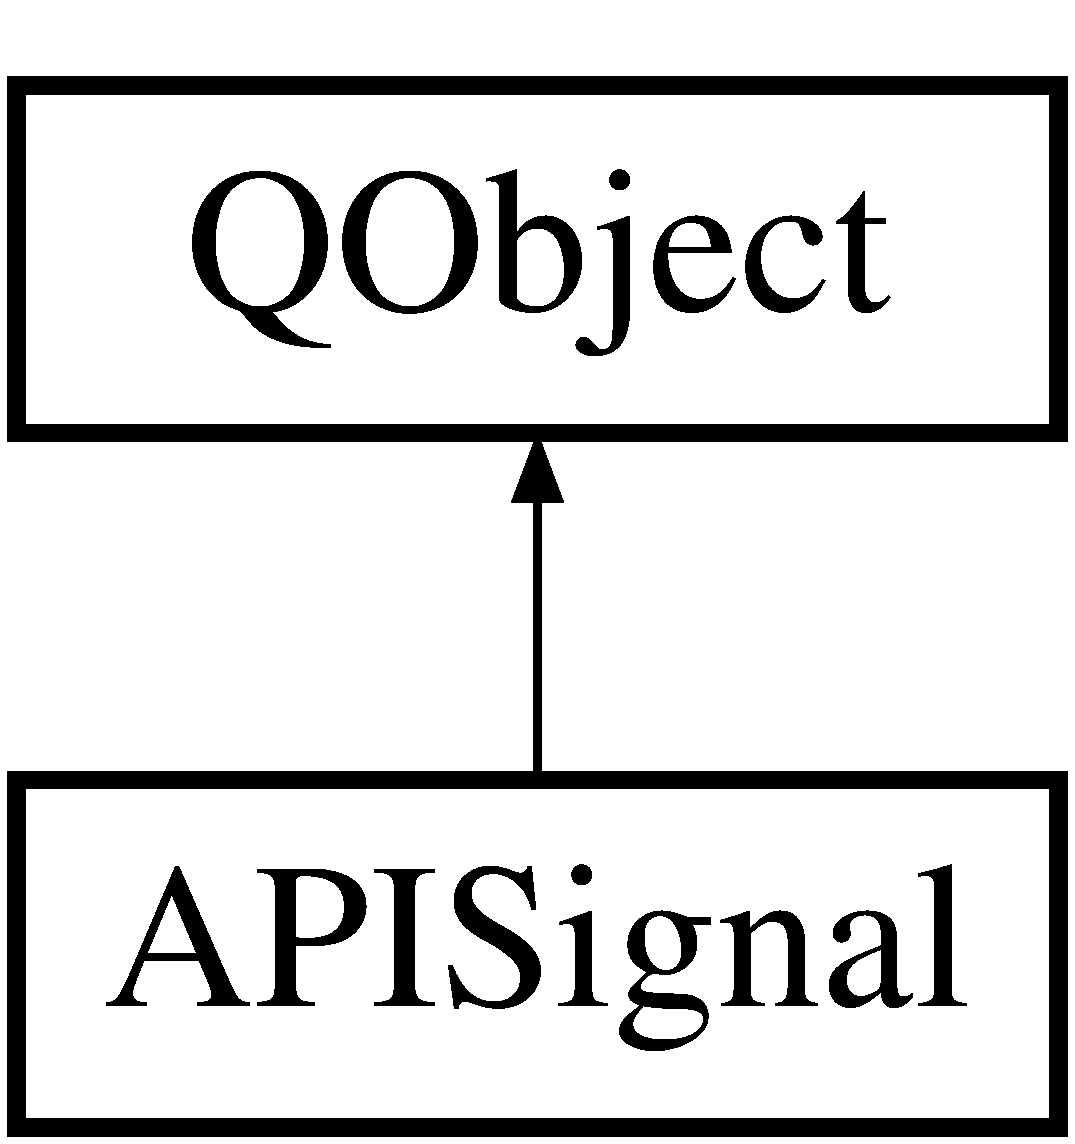
\includegraphics[height=2.000000cm]{class_a_p_i_signal}
\end{center}
\end{figure}
\subsection*{Public Slots}
\begin{DoxyCompactItemize}
\item 
\mbox{\Hypertarget{class_a_p_i_signal_aa39d78d40fce74c4adff19db446a34c8}\label{class_a_p_i_signal_aa39d78d40fce74c4adff19db446a34c8}} 
void {\bfseries handle\+Get\+Signal\+Aspect\+List} (const \hyperlink{class_a_p_i_request}{A\+P\+I\+Request} \&request, \hyperlink{class_a_p_i_response}{A\+P\+I\+Response} $\ast$response)
\item 
\mbox{\Hypertarget{class_a_p_i_signal_a0d698251dabf70472533fa99e4f53e48}\label{class_a_p_i_signal_a0d698251dabf70472533fa99e4f53e48}} 
void {\bfseries handle\+Get\+Signal\+Condition\+List} (const \hyperlink{class_a_p_i_request}{A\+P\+I\+Request} \&request, \hyperlink{class_a_p_i_response}{A\+P\+I\+Response} $\ast$response)
\end{DoxyCompactItemize}
\subsection*{Public Member Functions}
\begin{DoxyCompactItemize}
\item 
\mbox{\Hypertarget{class_a_p_i_signal_ab712db36d6e6281b9b317d60295ca3f6}\label{class_a_p_i_signal_ab712db36d6e6281b9b317d60295ca3f6}} 
{\bfseries A\+P\+I\+Signal} (Q\+Object $\ast$parent=nullptr)
\end{DoxyCompactItemize}


\subsection{Detailed Description}
\{get\} /api/signal\+\_\+aspect\+\_\+list\+:device\+ID Signal Aspect List  Signal\+Aspect\+List  Signal

\{Number\} device\+ID The signal\textquotesingle{}s Device ID.  Returns a list aspects defined for a signal sorted by sort\+Index. A Signal device uses this list to determine what state the L\+ED\textquotesingle{}s of a signal head should be set to (on, off or flashing). The signal starts at the first entry in this list and evaluates each signal condition entry assigned to this aspect (see /api/signal\+\_\+condition\+\_\+list). If all conditions of an aspect entry evaluate to true, the signal is set to that aspect. If none of the aspects evaluate to true, the signal sets the red L\+ED on and all others off.  \{Number\} device\+ID Signal\textquotesingle{}s device ID.  \{Number=0,1,2\} green\+Mode Green L\+ED state. 0 = off, 1 = on, 2 = flashing.  \{Number\} red\+Mode Red L\+ED state. 0 = off, 1 = on, 2 = flashing.  \{Number\} signal\+Aspect\+ID signal\+Aspect\textquotesingle{}s ID.  \{Number\} sort\+Index sort order.  \{Number\} yellow\+Mode Yellow L\+ED state. 0 = off, 1 = on, 2 = flashing.  Example usage\+: \href{http://localhost:8080/api/signal_aspect_list?deviceID=21}{\tt http\+://localhost\+:8080/api/signal\+\_\+aspect\+\_\+list?device\+I\+D=21}  \{json\} Success-\/\+Response\+: H\+T\+T\+P/1.\+1 200 OK \mbox{[}\{ \char`\"{}device\+I\+D\char`\"{}\+: \char`\"{}21\char`\"{}, \char`\"{}green\+Mode\char`\"{}\+: \char`\"{}1\char`\"{}, \char`\"{}red\+Mode\char`\"{}\+: \char`\"{}0\char`\"{}, \char`\"{}signal\+Aspect\+I\+D\char`\"{}\+: \char`\"{}5\char`\"{}, \char`\"{}sort\+Index\char`\"{}\+: \char`\"{}0\char`\"{}, \char`\"{}yellow\+Mode\char`\"{}\+: \char`\"{}0\char`\"{} \}, \{ \char`\"{}device\+I\+D\char`\"{}\+: \char`\"{}21\char`\"{}, \char`\"{}green\+Mode\char`\"{}\+: \char`\"{}2\char`\"{}, \char`\"{}red\+Mode\char`\"{}\+: \char`\"{}1\char`\"{}, \char`\"{}signal\+Aspect\+I\+D\char`\"{}\+: \char`\"{}6\char`\"{}, \char`\"{}sort\+Index\char`\"{}\+: \char`\"{}1\char`\"{}, \char`\"{}yellow\+Mode\char`\"{}\+: \char`\"{}0\char`\"{} \} \mbox{]}  \{get\} /api/signal\+\_\+condition\+\_\+list\+:aspect\+ID Aspect Condition List  Signal\+Aspect\+Condition\+List  Signal

\{Number\} aspect\+ID The aspect\textquotesingle{}s ID.  Returns a list conditions that must be met for the aspect to be valid (selected). All conditions in this list are evaluated by comparing the device\textquotesingle{}s current state specified by device\+ID to the entry\textquotesingle{}s device\+State using the condition\+Operand. If the comparison is successful the Signal Condition is considered to be true/valid. All conditions in the list must evaluate to true/valid for the aspect to be selected.  \{Number=0,1\} condition\+Operand Operand used for comparison. 0 = Equals, 1 = Not Equals.  \{Number=0,1,2\} device\+ID The ID of the device to be monitored.  \{Number\} device\+State The state the monitored device is compared to. When evaluated, this value is compared to the device\textquotesingle{}s current state.  \{Number\} signal\+Aspect\+ID signal\+Aspect\textquotesingle{}s ID.  \{Number\} signal\+Condition\+ID signal\+Condition\textquotesingle{}s ID.  Example usage\+: \href{http://localhost:8080/api/signal_condition_list?aspectID=6}{\tt http\+://localhost\+:8080/api/signal\+\_\+condition\+\_\+list?aspect\+I\+D=6}  \{json\} Success-\/\+Response\+: H\+T\+T\+P/1.\+1 200 OK \mbox{[}\{ \char`\"{}condition\+Operand\char`\"{}\+: \char`\"{}0\char`\"{}, \char`\"{}device\+I\+D\char`\"{}\+: \char`\"{}17\char`\"{}, \char`\"{}device\+State\char`\"{}\+: \char`\"{}3\char`\"{}, \char`\"{}signal\+Aspect\+I\+D\char`\"{}\+: \char`\"{}6\char`\"{}, \char`\"{}signal\+Condition\+I\+D\char`\"{}\+: \char`\"{}19\char`\"{} \}, \{ \char`\"{}condition\+Operand\char`\"{}\+: \char`\"{}0\char`\"{}, \char`\"{}device\+I\+D\char`\"{}\+: \char`\"{}18\char`\"{}, \char`\"{}device\+State\char`\"{}\+: \char`\"{}3\char`\"{}, \char`\"{}signal\+Aspect\+I\+D\char`\"{}\+: \char`\"{}6\char`\"{}, \char`\"{}signal\+Condition\+I\+D\char`\"{}\+: \char`\"{}20\char`\"{} \}, \{ \char`\"{}condition\+Operand\char`\"{}\+: \char`\"{}0\char`\"{}, \char`\"{}device\+I\+D\char`\"{}\+: \char`\"{}11\char`\"{}, \char`\"{}device\+State\char`\"{}\+: \char`\"{}1\char`\"{}, \char`\"{}signal\+Aspect\+I\+D\char`\"{}\+: \char`\"{}6\char`\"{}, \char`\"{}signal\+Condition\+I\+D\char`\"{}\+: \char`\"{}21\char`\"{} \}, \{ \char`\"{}condition\+Operand\char`\"{}\+: \char`\"{}0\char`\"{}, \char`\"{}device\+I\+D\char`\"{}\+: \char`\"{}5\char`\"{}, \char`\"{}device\+State\char`\"{}\+: \char`\"{}3\char`\"{}, \char`\"{}signal\+Aspect\+I\+D\char`\"{}\+: \char`\"{}6\char`\"{}, \char`\"{}signal\+Condition\+I\+D\char`\"{}\+: \char`\"{}22\char`\"{} \}, \{ \char`\"{}condition\+Operand\char`\"{}\+: \char`\"{}0\char`\"{}, \char`\"{}device\+I\+D\char`\"{}\+: \char`\"{}6\char`\"{}, \char`\"{}device\+State\char`\"{}\+: \char`\"{}3\char`\"{}, \char`\"{}signal\+Aspect\+I\+D\char`\"{}\+: \char`\"{}6\char`\"{}, \char`\"{}signal\+Condition\+I\+D\char`\"{}\+: \char`\"{}23\char`\"{} \}, \{ \char`\"{}condition\+Operand\char`\"{}\+: \char`\"{}0\char`\"{}, \char`\"{}device\+I\+D\char`\"{}\+: \char`\"{}8\char`\"{}, \char`\"{}device\+State\char`\"{}\+: \char`\"{}1\char`\"{}, \char`\"{}signal\+Aspect\+I\+D\char`\"{}\+: \char`\"{}6\char`\"{}, \char`\"{}signal\+Condition\+I\+D\char`\"{}\+: \char`\"{}24\char`\"{} \} \mbox{]} 

The documentation for this class was generated from the following files\+:\begin{DoxyCompactItemize}
\item 
L\+C\+S\+Server/A\+P\+I\+Signal.\+h\item 
L\+C\+S\+Server/A\+P\+I\+Signal.\+cpp\end{DoxyCompactItemize}

\hypertarget{class_a_p_i_turnout}{}\section{A\+P\+I\+Turnout Class Reference}
\label{class_a_p_i_turnout}\index{A\+P\+I\+Turnout@{A\+P\+I\+Turnout}}


{\ttfamily \#include $<$A\+P\+I\+Turnout.\+h$>$}

Inheritance diagram for A\+P\+I\+Turnout\+:\begin{figure}[H]
\begin{center}
\leavevmode
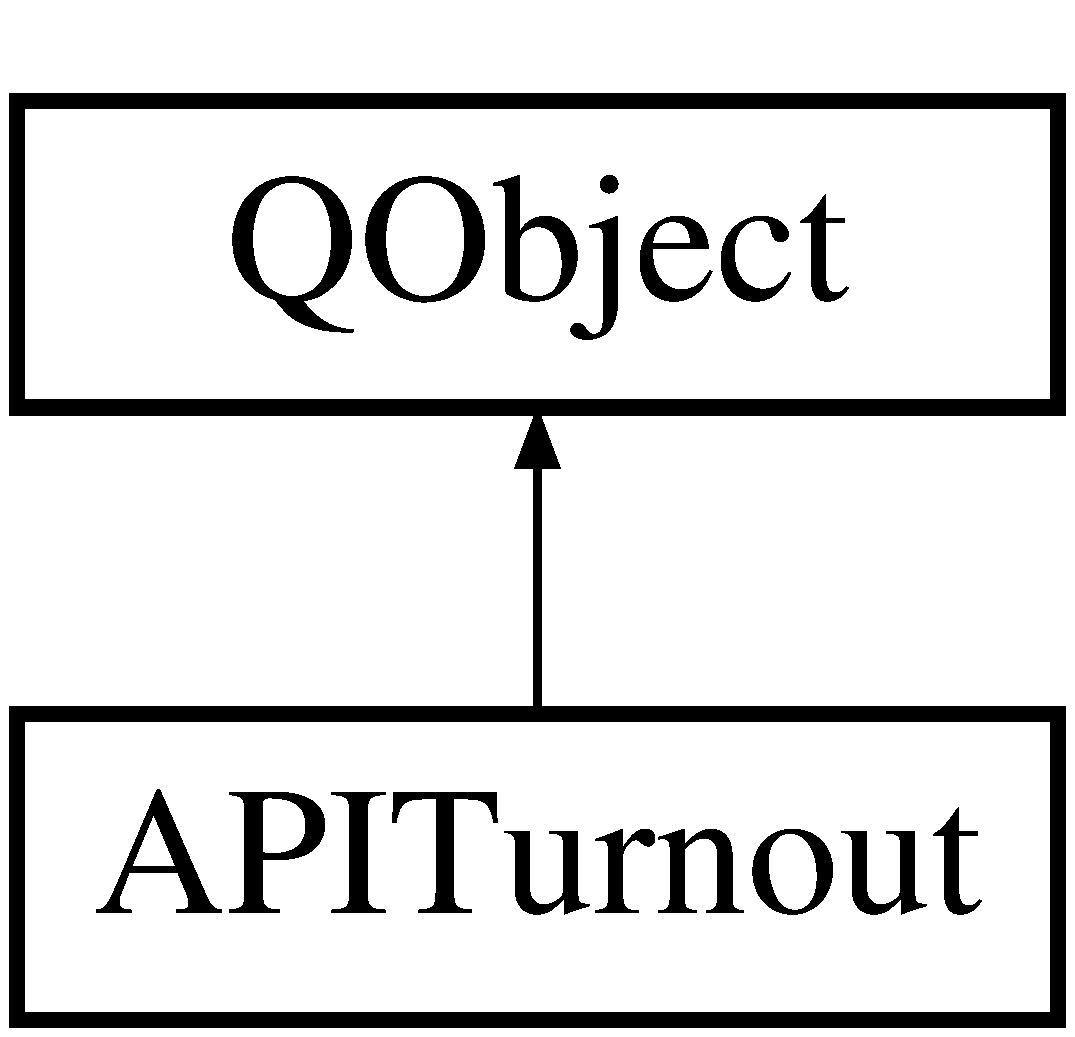
\includegraphics[height=2.000000cm]{class_a_p_i_turnout}
\end{center}
\end{figure}
\subsection*{Public Slots}
\begin{DoxyCompactItemize}
\item 
\mbox{\Hypertarget{class_a_p_i_turnout_a56cef33f12b9d8c13aa8cdce7e24bf0c}\label{class_a_p_i_turnout_a56cef33f12b9d8c13aa8cdce7e24bf0c}} 
void {\bfseries handle\+Activate\+Turnout\+Url} (const \hyperlink{class_a_p_i_request}{A\+P\+I\+Request} \&request, \hyperlink{class_a_p_i_response}{A\+P\+I\+Response} $\ast$response)
\end{DoxyCompactItemize}
\subsection*{Public Member Functions}
\begin{DoxyCompactItemize}
\item 
\mbox{\Hypertarget{class_a_p_i_turnout_a6c730f3cc2cee54be17e110770b9070b}\label{class_a_p_i_turnout_a6c730f3cc2cee54be17e110770b9070b}} 
{\bfseries A\+P\+I\+Turnout} (Q\+Object $\ast$parent=nullptr)
\end{DoxyCompactItemize}


\subsection{Detailed Description}
\{get\} /api/activate\+\_\+turnout\+:device\+ID,turnout\+State Activate Turnout  Activate\+Turnout  Turnout

\{Number\} device\+ID The turnout\textquotesingle{}s Device ID.  \{Number=1,3\} turnout\+State (optional) The desired state to set the turnout to.  Sets the turnout to the desired state (direction) 1 = Normal 2 = Diverging. If no state is specified, the turnout is toggled between normal and thrown.  Example usage\+: \href{http://localhost:8080/api/activate_turnout?deviceID=7&turnoutState=3}{\tt http\+://localhost\+:8080/api/activate\+\_\+turnout?device\+I\+D=7\&turnout\+State=3}  \{get\} /controller/device/config\+:device\+ID Download Configuration  Turnout\+Configuration  Turnout

\{Number\} device\+ID The turnout\textquotesingle{}s Device ID.  Download the turnout\textquotesingle{}s configuration. I\+N\+P\+U\+T\+P\+IN and M\+O\+T\+O\+R\+P\+IN entries control how the device handles the pin. If set to 1, the pin order is reversed. This is useful if the wires are connected backwards to the motor and/or the input pins. Usually, both of these entries are set together, meaning, if M\+O\+T\+O\+R\+P\+IN is set to 1 set I\+N\+P\+U\+T\+P\+IN to 1 as well. The routes list is used by the device to determine what direction the turnout should be set to in response to a T\+R\+N\+\_\+\+A\+C\+T\+I\+V\+A\+T\+E\+\_\+\+R\+O\+U\+TE message.  Example usage. This example returns the configuration for a Turnout Device\+: \href{http://localhost:8080/controller/device/config?deviceID=1}{\tt http\+://localhost\+:8080/controller/device/config?device\+I\+D=1}  \{json\} Success-\/\+Response\+: H\+T\+T\+P/1.\+1 200 OK \{ \char`\"{}\+I\+N\+P\+U\+T\+P\+I\+N\char`\"{}\+: \char`\"{}1\char`\"{}, \char`\"{}\+M\+O\+T\+O\+R\+P\+I\+N\char`\"{}\+: \char`\"{}1\char`\"{}, \char`\"{}device\+Class\char`\"{}\+: \char`\"{}1\char`\"{}, \char`\"{}routes\char`\"{}\+: \mbox{[}\{ \char`\"{}route\+I\+D\char`\"{}\+: \char`\"{}1\char`\"{}, \char`\"{}turnout\+State\char`\"{}\+: \char`\"{}1\char`\"{} \}, \{ \char`\"{}route\+I\+D\char`\"{}\+: \char`\"{}2\char`\"{}, \char`\"{}turnout\+State\char`\"{}\+: \char`\"{}1\char`\"{} \}, \{ \char`\"{}route\+I\+D\char`\"{}\+: \char`\"{}3\char`\"{}, \char`\"{}turnout\+State\char`\"{}\+: \char`\"{}3\char`\"{} \}, \{ \char`\"{}route\+I\+D\char`\"{}\+: \char`\"{}4\char`\"{}, \char`\"{}turnout\+State\char`\"{}\+: \char`\"{}3\char`\"{} \} \mbox{]} \} 

The documentation for this class was generated from the following files\+:\begin{DoxyCompactItemize}
\item 
L\+C\+S\+Server/A\+P\+I\+Turnout.\+h\item 
L\+C\+S\+Server/A\+P\+I\+Turnout.\+cpp\end{DoxyCompactItemize}

\hypertarget{class_app_service}{}\section{App\+Service Class Reference}
\label{class_app_service}\index{App\+Service@{App\+Service}}
Inheritance diagram for App\+Service\+:\begin{figure}[H]
\begin{center}
\leavevmode
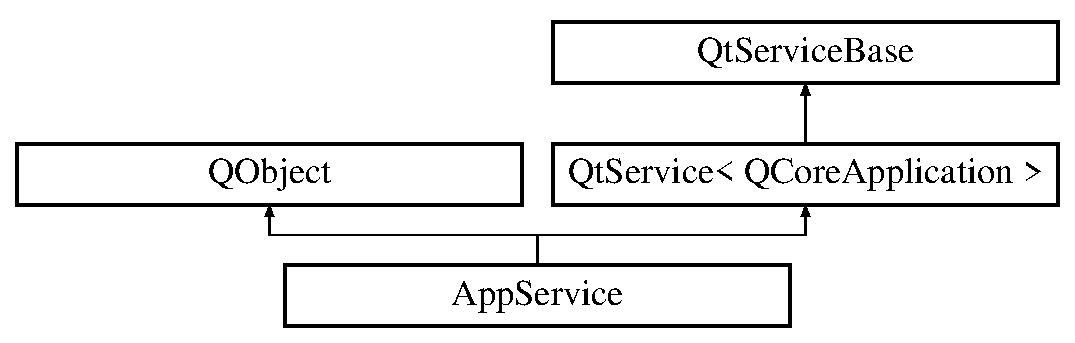
\includegraphics[height=3.000000cm]{class_app_service}
\end{center}
\end{figure}
\subsection*{Public Member Functions}
\begin{DoxyCompactItemize}
\item 
\mbox{\Hypertarget{class_app_service_a1b8bee1f7ab6d64ccfb9f23ff716a850}\label{class_app_service_a1b8bee1f7ab6d64ccfb9f23ff716a850}} 
{\bfseries App\+Service} (int argc, char $\ast$$\ast$argv, const Q\+String \&name, const Q\+String \&description)
\item 
\mbox{\Hypertarget{class_app_service_ace4bde07e05766553435a751b917d903}\label{class_app_service_ace4bde07e05766553435a751b917d903}} 
void {\bfseries initiate\+Stop} (void)
\item 
\mbox{\Hypertarget{class_app_service_a63c7beff040e1cf6f33ad53c85824aac}\label{class_app_service_a63c7beff040e1cf6f33ad53c85824aac}} 
void {\bfseries start\+Simulator} (void)
\end{DoxyCompactItemize}
\subsection*{Protected Slots}
\begin{DoxyCompactItemize}
\item 
\mbox{\Hypertarget{class_app_service_a21368cb3a7a25ef34d78138d14434fea}\label{class_app_service_a21368cb3a7a25ef34d78138d14434fea}} 
void {\bfseries timer\+Proc} (void)
\item 
\mbox{\Hypertarget{class_app_service_aea5d544b09bb238e36d1ce86726063e7}\label{class_app_service_aea5d544b09bb238e36d1ce86726063e7}} 
void {\bfseries stop\+Timer\+Proc} (void)
\item 
\mbox{\Hypertarget{class_app_service_aebb27134691e5afb7ebe770c258a4295}\label{class_app_service_aebb27134691e5afb7ebe770c258a4295}} 
void {\bfseries shutdown\+Monitor} (int pin, int value)
\item 
\mbox{\Hypertarget{class_app_service_ae3ae8f61a6e545232cbcf12d4009c882}\label{class_app_service_ae3ae8f61a6e545232cbcf12d4009c882}} 
void {\bfseries about\+To\+Quit} (void)
\end{DoxyCompactItemize}
\subsection*{Protected Member Functions}
\begin{DoxyCompactItemize}
\item 
\mbox{\Hypertarget{class_app_service_aef117ff830f4d07806f22a352edf9fd6}\label{class_app_service_aef117ff830f4d07806f22a352edf9fd6}} 
void {\bfseries start\+Web\+Server} (void)
\item 
void \hyperlink{class_app_service_a987c81ba936b7ce15b84cba99851dabb}{start} (void)
\item 
void \hyperlink{class_app_service_a343b5fb7522b24f9fc6dd2aeda940f01}{stop} (void)
\end{DoxyCompactItemize}
\subsection*{Additional Inherited Members}


\subsection{Member Function Documentation}
\mbox{\Hypertarget{class_app_service_a987c81ba936b7ce15b84cba99851dabb}\label{class_app_service_a987c81ba936b7ce15b84cba99851dabb}} 
\index{App\+Service@{App\+Service}!start@{start}}
\index{start@{start}!App\+Service@{App\+Service}}
\subsubsection{\texorpdfstring{start()}{start()}}
{\footnotesize\ttfamily void App\+Service\+::start (\begin{DoxyParamCaption}\item[{void}]{ }\end{DoxyParamCaption})\hspace{0.3cm}{\ttfamily [protected]}, {\ttfamily [virtual]}}

This function must be implemented in \hyperlink{class_qt_service_base}{Qt\+Service\+Base} subclasses in order to perform the service\textquotesingle{}s work. Usually you create some main object on the heap which is the heart of your service.

The function is only called when no service specific arguments were passed to the service constructor, and is called by \hyperlink{class_qt_service_base_afae2e589de71c1ae3ae8db3dc9ab9c64}{exec()} after it has called the \hyperlink{class_qt_service_a84f5f60304117e1f11cc0ed16dc0b72e}{execute\+Application()} function.

Note that you {\itshape don\textquotesingle{}t} need to create an application object or call its \hyperlink{class_qt_service_base_afae2e589de71c1ae3ae8db3dc9ab9c64}{exec()} function explicitly.

\begin{DoxySeeAlso}{See also}
\hyperlink{class_qt_service_base_afae2e589de71c1ae3ae8db3dc9ab9c64}{exec()}, \hyperlink{class_app_service_a343b5fb7522b24f9fc6dd2aeda940f01}{stop()}, \hyperlink{class_qt_service_controller_a5e9d6da5081d70f31611456d0ef0687e}{Qt\+Service\+Controller\+::start()} 
\end{DoxySeeAlso}


Implements \hyperlink{class_qt_service_base_adbc0cd621b41bd3a6a1f62fda432e9e4}{Qt\+Service\+Base}.

\mbox{\Hypertarget{class_app_service_a343b5fb7522b24f9fc6dd2aeda940f01}\label{class_app_service_a343b5fb7522b24f9fc6dd2aeda940f01}} 
\index{App\+Service@{App\+Service}!stop@{stop}}
\index{stop@{stop}!App\+Service@{App\+Service}}
\subsubsection{\texorpdfstring{stop()}{stop()}}
{\footnotesize\ttfamily void App\+Service\+::stop (\begin{DoxyParamCaption}\item[{void}]{ }\end{DoxyParamCaption})\hspace{0.3cm}{\ttfamily [protected]}, {\ttfamily [virtual]}}

Reimplement this function to perform additional cleanups before shutting down (for example deleting a main object if it was created in the \hyperlink{class_app_service_a987c81ba936b7ce15b84cba99851dabb}{start()} function).

This function is called in reply to controller requests. The default implementation does nothing.

\begin{DoxySeeAlso}{See also}
\hyperlink{class_app_service_a987c81ba936b7ce15b84cba99851dabb}{start()}, \hyperlink{class_qt_service_controller_ad06afa647666769e309474b18bf7cf90}{Qt\+Service\+Controller\+::stop()} 
\end{DoxySeeAlso}


Reimplemented from \hyperlink{class_qt_service_base_a8d52c1b8fd06b50bdc0a0c6f9936a68e}{Qt\+Service\+Base}.



The documentation for this class was generated from the following files\+:\begin{DoxyCompactItemize}
\item 
L\+C\+S\+Server/App\+Service.\+h\item 
L\+C\+S\+Server/App\+Service.\+cpp\end{DoxyCompactItemize}

\hypertarget{class_controller_entry}{}\section{Controller\+Entry Class Reference}
\label{class_controller_entry}\index{Controller\+Entry@{Controller\+Entry}}
\subsection*{Public Member Functions}
\begin{DoxyCompactItemize}
\item 
\mbox{\Hypertarget{class_controller_entry_a26793ef5e3046aba4d50a10faf4a3d28}\label{class_controller_entry_a26793ef5e3046aba4d50a10faf4a3d28}} 
{\bfseries Controller\+Entry} (const \hyperlink{class_controller_entry}{Controller\+Entry} \&other)
\item 
\mbox{\Hypertarget{class_controller_entry_af209c8df410096b335c3eda85cb13cbe}\label{class_controller_entry_af209c8df410096b335c3eda85cb13cbe}} 
long {\bfseries get\+Serial\+Number} (void) const
\item 
\mbox{\Hypertarget{class_controller_entry_a71eea08af0193dca797148f8dc375143}\label{class_controller_entry_a71eea08af0193dca797148f8dc375143}} 
void {\bfseries set\+Serial\+Number} (long value)
\item 
\mbox{\Hypertarget{class_controller_entry_a118aec7c94dfddb49a0c4753cd7fc482}\label{class_controller_entry_a118aec7c94dfddb49a0c4753cd7fc482}} 
int {\bfseries get\+Controller\+ID} (void) const
\item 
\mbox{\Hypertarget{class_controller_entry_ad25f5d4cd7c78d8bfaa94b6bd4930c1b}\label{class_controller_entry_ad25f5d4cd7c78d8bfaa94b6bd4930c1b}} 
void {\bfseries set\+Controller\+ID} (int value)
\item 
\mbox{\Hypertarget{class_controller_entry_a5b981f25f7e3a9a50817a70959096766}\label{class_controller_entry_a5b981f25f7e3a9a50817a70959096766}} 
\hyperlink{_global_defs_8h_a51207b6a49e0da6f9978a3019d93480a}{Controller\+Status\+Enum} {\bfseries get\+Status} (void) const
\item 
\mbox{\Hypertarget{class_controller_entry_a3b937ec9d808aacc509304ab0fa58959}\label{class_controller_entry_a3b937ec9d808aacc509304ab0fa58959}} 
void {\bfseries set\+Status} (\hyperlink{_global_defs_8h_a51207b6a49e0da6f9978a3019d93480a}{Controller\+Status\+Enum} value)
\item 
\mbox{\Hypertarget{class_controller_entry_ab3897317445003f2776d4c3ae54f621f}\label{class_controller_entry_ab3897317445003f2776d4c3ae54f621f}} 
Q\+String {\bfseries get\+Version} (void) const
\item 
\mbox{\Hypertarget{class_controller_entry_a2eb241a6eacde27c5d2f23e71104f210}\label{class_controller_entry_a2eb241a6eacde27c5d2f23e71104f210}} 
void {\bfseries set\+Version} (int major, int minor, int build)
\item 
\mbox{\Hypertarget{class_controller_entry_ab761e0059786897f281c3ef9d03d80fe}\label{class_controller_entry_ab761e0059786897f281c3ef9d03d80fe}} 
void {\bfseries operator=} (const \hyperlink{class_controller_entry}{Controller\+Entry} \&other)
\end{DoxyCompactItemize}


The documentation for this class was generated from the following file\+:\begin{DoxyCompactItemize}
\item 
L\+C\+S\+Server/Controller\+Manager.\+cpp\end{DoxyCompactItemize}

\hypertarget{class_controller_manager}{}\section{Controller\+Manager Class Reference}
\label{class_controller_manager}\index{Controller\+Manager@{Controller\+Manager}}


Singleton class monitoring the current state of controllers.  




{\ttfamily \#include $<$Controller\+Manager.\+h$>$}

Inheritance diagram for Controller\+Manager\+:\begin{figure}[H]
\begin{center}
\leavevmode
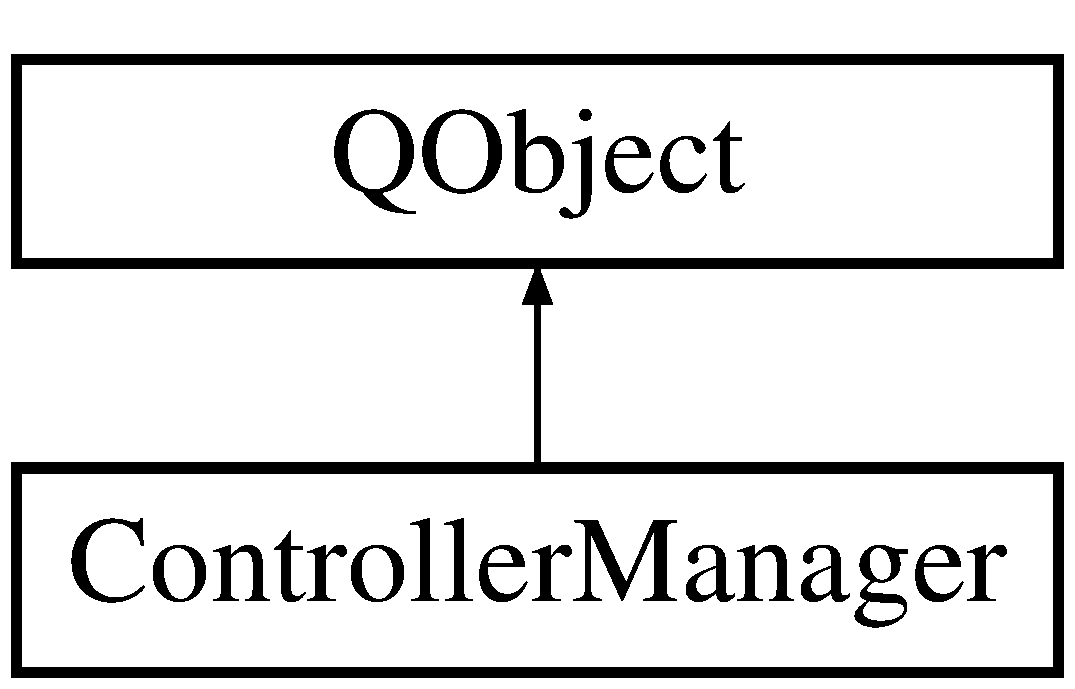
\includegraphics[height=2.000000cm]{class_controller_manager}
\end{center}
\end{figure}
\subsection*{Public Slots}
\begin{DoxyCompactItemize}
\item 
\mbox{\Hypertarget{class_controller_manager_a5b496ff2650f4048dc91de9cdeea43c8}\label{class_controller_manager_a5b496ff2650f4048dc91de9cdeea43c8}} 
unsigned long \hyperlink{class_controller_manager_a5b496ff2650f4048dc91de9cdeea43c8}{get\+Serial\+Number} (int controller\+ID)
\begin{DoxyCompactList}\small\item\em Returns the serial number for the given controller\+ID. \end{DoxyCompactList}\end{DoxyCompactItemize}
\subsection*{Signals}
\begin{DoxyCompactItemize}
\item 
\mbox{\Hypertarget{class_controller_manager_a38c42bcc777c296ff2e0e4c4099dbdf7}\label{class_controller_manager_a38c42bcc777c296ff2e0e4c4099dbdf7}} 
void \hyperlink{class_controller_manager_a38c42bcc777c296ff2e0e4c4099dbdf7}{controller\+Added} (long serial\+Number)
\begin{DoxyCompactList}\small\item\em Emitted when a S\+Y\+S\+\_\+\+C\+O\+N\+T\+R\+O\+L\+L\+E\+R\+\_\+\+O\+N\+L\+I\+NE U\+DP message is received. \end{DoxyCompactList}\item 
\mbox{\Hypertarget{class_controller_manager_aaca6003c9cc1a0c184932fd4b2649b8a}\label{class_controller_manager_aaca6003c9cc1a0c184932fd4b2649b8a}} 
void \hyperlink{class_controller_manager_aaca6003c9cc1a0c184932fd4b2649b8a}{controller\+Removed} (long serial\+Number)
\begin{DoxyCompactList}\small\item\em Currently, this signal is not emitted as there is no way (currently) for the detection of a controller going offline. \end{DoxyCompactList}\item 
\mbox{\Hypertarget{class_controller_manager_ad065b1ffd21f4f5e2a84b4ce15bf404a}\label{class_controller_manager_ad065b1ffd21f4f5e2a84b4ce15bf404a}} 
void \hyperlink{class_controller_manager_ad065b1ffd21f4f5e2a84b4ce15bf404a}{controller\+Status\+Changed} (long serial\+Number, \hyperlink{_global_defs_8h_a51207b6a49e0da6f9978a3019d93480a}{Controller\+Status\+Enum} new\+Status)
\begin{DoxyCompactList}\small\item\em Emitted when a S\+Y\+S\+\_\+\+C\+O\+N\+T\+R\+O\+L\+L\+E\+R\+\_\+\+O\+N\+L\+I\+NE and S\+Y\+S\+\_\+\+R\+E\+S\+T\+A\+R\+T\+I\+NG U\+DP messages are received. \end{DoxyCompactList}\end{DoxyCompactItemize}
\subsection*{Public Member Functions}
\begin{DoxyCompactItemize}
\item 
\mbox{\Hypertarget{class_controller_manager_a74516f22a00c40a20dbd08ffcd8777d6}\label{class_controller_manager_a74516f22a00c40a20dbd08ffcd8777d6}} 
\hyperlink{class_controller_manager_a74516f22a00c40a20dbd08ffcd8777d6}{$\sim$\+Controller\+Manager} (void)
\begin{DoxyCompactList}\small\item\em Deststructor. \end{DoxyCompactList}\item 
\mbox{\Hypertarget{class_controller_manager_a140123d13332dba6947846924c666714}\label{class_controller_manager_a140123d13332dba6947846924c666714}} 
long \hyperlink{class_controller_manager_a140123d13332dba6947846924c666714}{get\+Connection\+Serial\+Number} (int index) const
\begin{DoxyCompactList}\small\item\em Returns the controller\textquotesingle{}s serial number at the given index. \end{DoxyCompactList}\item 
void \hyperlink{class_controller_manager_a09aae80f5783ab2cb0da0ba39144ddf6}{get\+Connected\+Info} (long serial\+Number, Q\+String \&version, \hyperlink{_global_defs_8h_a51207b6a49e0da6f9978a3019d93480a}{Controller\+Status\+Enum} \&status)
\item 
\mbox{\Hypertarget{class_controller_manager_ae195bc494eb3d3afeabc4e71471497d3}\label{class_controller_manager_ae195bc494eb3d3afeabc4e71471497d3}} 
int \hyperlink{class_controller_manager_ae195bc494eb3d3afeabc4e71471497d3}{get\+Connection\+Count} (void) const
\begin{DoxyCompactList}\small\item\em Returns the count of connected controllers. \end{DoxyCompactList}\end{DoxyCompactItemize}
\subsection*{Static Public Member Functions}
\begin{DoxyCompactItemize}
\item 
\mbox{\Hypertarget{class_controller_manager_a3f4999812436ab587f8ec2ee11128c51}\label{class_controller_manager_a3f4999812436ab587f8ec2ee11128c51}} 
static \hyperlink{class_controller_manager}{Controller\+Manager} $\ast$ \hyperlink{class_controller_manager_a3f4999812436ab587f8ec2ee11128c51}{instance} (void)
\begin{DoxyCompactList}\small\item\em Returns/creates the singleton instance. \end{DoxyCompactList}\end{DoxyCompactItemize}
\subsection*{Protected Slots}
\begin{DoxyCompactItemize}
\item 
\mbox{\Hypertarget{class_controller_manager_a5e9480ad4b88ff536ab60dbc9cb6619f}\label{class_controller_manager_a5e9480ad4b88ff536ab60dbc9cb6619f}} 
void \hyperlink{class_controller_manager_a5e9480ad4b88ff536ab60dbc9cb6619f}{new\+U\+D\+P\+Message} (const \hyperlink{class_u_d_p_message}{U\+D\+P\+Message} \&message)
\begin{DoxyCompactList}\small\item\em U\+DP Message handler. \end{DoxyCompactList}\end{DoxyCompactItemize}


\subsection{Detailed Description}
Singleton class monitoring the current state of controllers. 

\hyperlink{class_controller_manager}{Controller\+Manager} This class monitors U\+DP messages collecting information about the current state of L\+CS controllers. When a controller\textquotesingle{}s online status changes, a controller\+Status\+Changed signal is emitted. On a S\+Y\+S\+\_\+\+C\+O\+N\+T\+R\+O\+L\+L\+E\+R\+\_\+\+O\+N\+L\+I\+NE message, the controller\+Added signal is emitted. 

\subsection{Member Function Documentation}
\mbox{\Hypertarget{class_controller_manager_a09aae80f5783ab2cb0da0ba39144ddf6}\label{class_controller_manager_a09aae80f5783ab2cb0da0ba39144ddf6}} 
\index{Controller\+Manager@{Controller\+Manager}!get\+Connected\+Info@{get\+Connected\+Info}}
\index{get\+Connected\+Info@{get\+Connected\+Info}!Controller\+Manager@{Controller\+Manager}}
\subsubsection{\texorpdfstring{get\+Connected\+Info()}{getConnectedInfo()}}
{\footnotesize\ttfamily void Controller\+Manager\+::get\+Connected\+Info (\begin{DoxyParamCaption}\item[{long}]{serial\+Number,  }\item[{Q\+String \&}]{version,  }\item[{\hyperlink{_global_defs_8h_a51207b6a49e0da6f9978a3019d93480a}{Controller\+Status\+Enum} \&}]{status }\end{DoxyParamCaption})}

Fills version and status with the current information for a controller. 
\begin{DoxyParams}{Parameters}
{\em serial\+Number} & long Serial number of the controller to lookup. \\
\hline
\end{DoxyParams}


The documentation for this class was generated from the following files\+:\begin{DoxyCompactItemize}
\item 
L\+C\+S\+Server/Controller\+Manager.\+h\item 
L\+C\+S\+Server/Controller\+Manager.\+cpp\end{DoxyCompactItemize}

\hypertarget{class_database}{}\section{Database Class Reference}
\label{class_database}\index{Database@{Database}}
Inheritance diagram for Database\+:\begin{figure}[H]
\begin{center}
\leavevmode
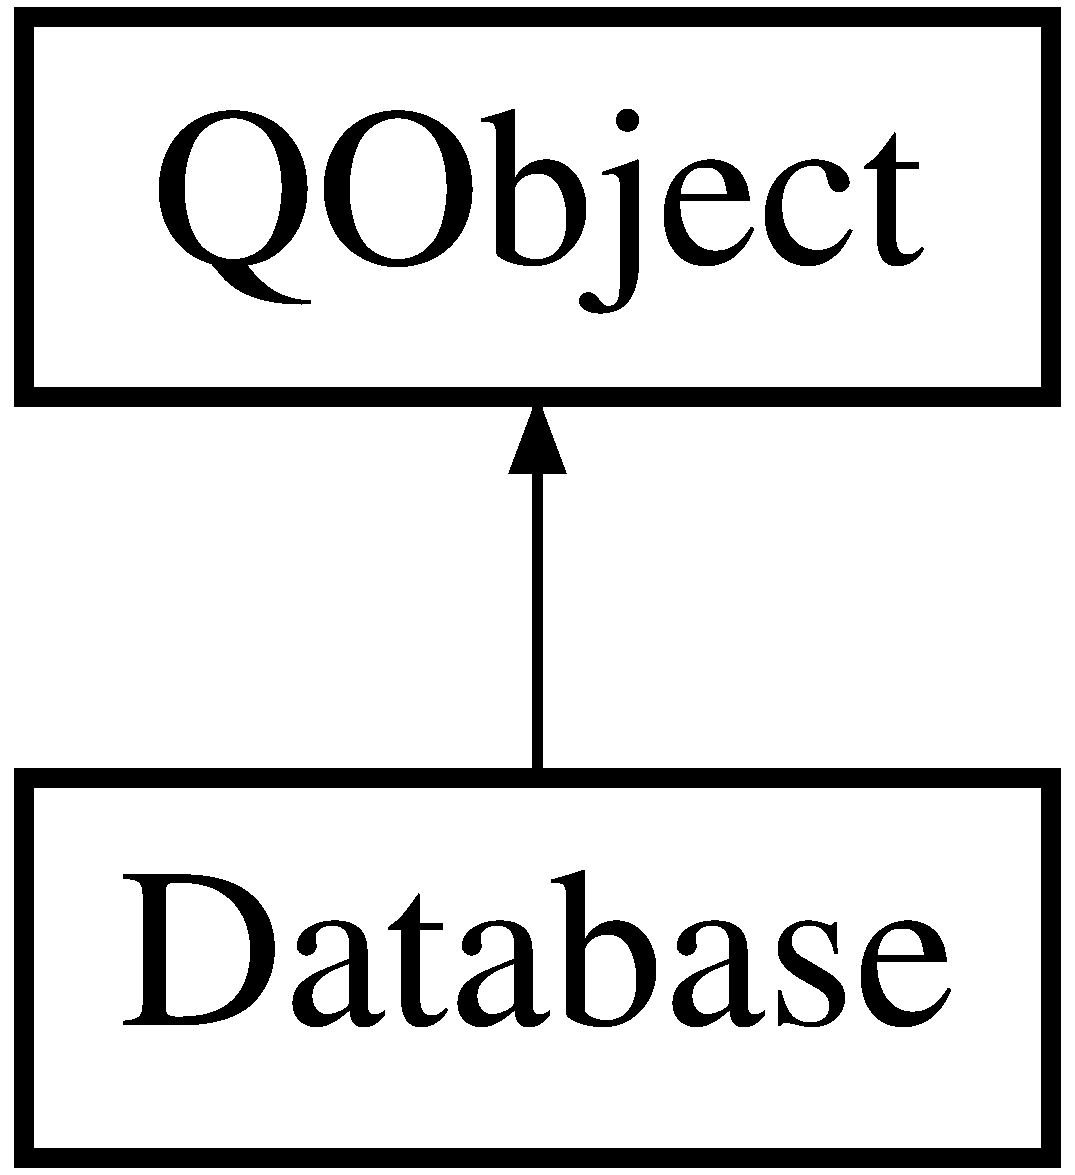
\includegraphics[height=2.000000cm]{class_database}
\end{center}
\end{figure}
\subsection*{Signals}
\begin{DoxyCompactItemize}
\item 
\mbox{\Hypertarget{class_database_ab65267ed41ba9a21b7f1abd5e738d2a0}\label{class_database_ab65267ed41ba9a21b7f1abd5e738d2a0}} 
void {\bfseries log\+Error} (int category, int code, const Q\+String \&error\+Text)
\end{DoxyCompactItemize}
\subsection*{Public Member Functions}
\begin{DoxyCompactItemize}
\item 
\mbox{\Hypertarget{class_database_a1eb00cb7d192abcfa766f6228492ff23}\label{class_database_a1eb00cb7d192abcfa766f6228492ff23}} 
{\bfseries Database} (Q\+Object $\ast$parent=0)
\item 
\mbox{\Hypertarget{class_database_aa2c92e707d102550af16c8dca42815ac}\label{class_database_aa2c92e707d102550af16c8dca42815ac}} 
bool {\bfseries init} (const Q\+String \&path\+And\+File)
\item 
\mbox{\Hypertarget{class_database_a53105764e2c9c0992e0e95022046288f}\label{class_database_a53105764e2c9c0992e0e95022046288f}} 
void {\bfseries remove\+Database} (void)
\item 
\mbox{\Hypertarget{class_database_aff7b80a2cf6743c0a57f63d9bfed641b}\label{class_database_aff7b80a2cf6743c0a57f63d9bfed641b}} 
bool {\bfseries check\+Database} (void)
\item 
\mbox{\Hypertarget{class_database_ab916411c9403523dd709de378026754d}\label{class_database_ab916411c9403523dd709de378026754d}} 
bool {\bfseries create\+Database} (void)
\item 
\mbox{\Hypertarget{class_database_a4eaffbc1571e91a8adb40cfe076069c5}\label{class_database_a4eaffbc1571e91a8adb40cfe076069c5}} 
int {\bfseries get\+Controller\+ID} (long serial\+Number)
\item 
\mbox{\Hypertarget{class_database_a49c87a6a938b5b0027cb3d7e95a2fdd8}\label{class_database_a49c87a6a938b5b0027cb3d7e95a2fdd8}} 
unsigned long {\bfseries get\+Serial\+Number} (int controller\+ID)
\item 
\mbox{\Hypertarget{class_database_aebd4c272f7a8331f46c57105aae3cf31}\label{class_database_aebd4c272f7a8331f46c57105aae3cf31}} 
int {\bfseries add\+Controller} (int controller\+Class, const Q\+String \&controller\+Name, const Q\+String \&controller\+Description)
\item 
\mbox{\Hypertarget{class_database_ad022e230c02d99968e1b521c24548269}\label{class_database_ad022e230c02d99968e1b521c24548269}} 
Q\+Sql\+Database {\bfseries get\+Database} (void) const
\item 
\mbox{\Hypertarget{class_database_a1c19214e960ef7e6e06cf8bc8a96dd13}\label{class_database_a1c19214e960ef7e6e06cf8bc8a96dd13}} 
int {\bfseries get\+Next\+ID} (const Q\+String \&table\+Name)
\item 
\mbox{\Hypertarget{class_database_a40123ea0706f6bd80a66f4c03026aaae}\label{class_database_a40123ea0706f6bd80a66f4c03026aaae}} 
int {\bfseries get\+D\+B\+Version} (void)
\item 
\mbox{\Hypertarget{class_database_ac661c2459b9a7ac22c882971be8ee3b8}\label{class_database_ac661c2459b9a7ac22c882971be8ee3b8}} 
void {\bfseries set\+D\+B\+Version} (int new\+Version)
\item 
\mbox{\Hypertarget{class_database_ae92b8bfa260ee01d7e2bb411917f3049}\label{class_database_ae92b8bfa260ee01d7e2bb411917f3049}} 
Q\+Byte\+Array {\bfseries get\+Multi\+Controller\+Config} (quint32 serial\+Number)
\item 
\mbox{\Hypertarget{class_database_aa458cd303347f4f10b74c2c9b3661084}\label{class_database_aa458cd303347f4f10b74c2c9b3661084}} 
Q\+Json\+Array {\bfseries get\+Notification\+List} (quint32 serial\+Number)
\item 
\mbox{\Hypertarget{class_database_aaabd22c307d3bdb68148296d636758cf}\label{class_database_aaabd22c307d3bdb68148296d636758cf}} 
Q\+Byte\+Array {\bfseries get\+Controller\+Module\+Config} (quint32 serial\+Number, quint32 address)
\item 
\mbox{\Hypertarget{class_database_a702c94a5d8c9796ad5e4e216ae9278fa}\label{class_database_a702c94a5d8c9796ad5e4e216ae9278fa}} 
Q\+String {\bfseries get\+Device\+Config} (int device\+ID)
\item 
\mbox{\Hypertarget{class_database_a26943586c348a996d31c722cd10c8bc2}\label{class_database_a26943586c348a996d31c722cd10c8bc2}} 
void {\bfseries get\+Device\+Properties} (int device\+ID, Q\+Json\+Object \&device)
\item 
\mbox{\Hypertarget{class_database_a26992f37246c3c2383716704398c3403}\label{class_database_a26992f37246c3c2383716704398c3403}} 
void {\bfseries get\+Turnout\+Config} (int device\+ID, Q\+Json\+Object \&device)
\item 
\mbox{\Hypertarget{class_database_a14e593519bd9fe8c414083d633906786}\label{class_database_a14e593519bd9fe8c414083d633906786}} 
void {\bfseries get\+Signal\+Config} (int device\+ID, Q\+Json\+Object \&device)
\item 
\mbox{\Hypertarget{class_database_a13557f1cf9e0ea0b12d73652686dcee5}\label{class_database_a13557f1cf9e0ea0b12d73652686dcee5}} 
Q\+String {\bfseries get\+Signal\+Aspect\+Config} (int aspect\+ID)
\item 
\mbox{\Hypertarget{class_database_a015c1d3e3c83c9c66fe4f86dbff656a6}\label{class_database_a015c1d3e3c83c9c66fe4f86dbff656a6}} 
Q\+String {\bfseries get\+Turnout\+Name} (int device\+ID)
\item 
\mbox{\Hypertarget{class_database_aefd61c538939ce9b79c85c2df6914447}\label{class_database_aefd61c538939ce9b79c85c2df6914447}} 
int {\bfseries getdevice\+ID} (const Q\+String \&name)
\item 
\mbox{\Hypertarget{class_database_aaa5f3cfe0c9dc902c3e8d688e8f954d7}\label{class_database_aaa5f3cfe0c9dc902c3e8d688e8f954d7}} 
\hyperlink{_global_defs_8h_ad17679fac69973be9b3a2787a60d7722}{Device\+Class\+Enum} {\bfseries get\+Device\+Class} (int device\+ID)
\item 
\mbox{\Hypertarget{class_database_a34aaa93240ff4b005b10e44ba1c6eaba}\label{class_database_a34aaa93240ff4b005b10e44ba1c6eaba}} 
Q\+List$<$ int $>$ {\bfseries get\+Exclude\+Route\+List} (int route\+ID)
\item 
\mbox{\Hypertarget{class_database_a52a865e7e0e177dab5c0a451f37a1d1a}\label{class_database_a52a865e7e0e177dab5c0a451f37a1d1a}} 
void {\bfseries get\+Controller\+I\+D\+And\+Name} (quint32 serial\+Number, int \&device\+ID, Q\+String \&controller\+Name)
\item 
\mbox{\Hypertarget{class_database_a1d17037c1dfaa2f67327ae0297d4567a}\label{class_database_a1d17037c1dfaa2f67327ae0297d4567a}} 
Q\+Json\+Object {\bfseries fetch\+Item} (const Q\+String \&query\+String)
\item 
\mbox{\Hypertarget{class_database_a1b1bd2990fdc80d0f4ed51f571966272}\label{class_database_a1b1bd2990fdc80d0f4ed51f571966272}} 
Q\+Json\+Array {\bfseries fetch\+Items} (const Q\+String \&query\+String)
\item 
\mbox{\Hypertarget{class_database_a82058cf13df09949bc4f6e28ce4931ba}\label{class_database_a82058cf13df09949bc4f6e28ce4931ba}} 
Q\+Json\+Object {\bfseries create\+Json\+Object} (Q\+Sql\+Query \&query)
\item 
\mbox{\Hypertarget{class_database_a27d4e89a6c9e7bdd79a4548dcc0bafa7}\label{class_database_a27d4e89a6c9e7bdd79a4548dcc0bafa7}} 
Q\+Json\+Array {\bfseries create\+Json\+Array} (Q\+Sql\+Query \&query)
\item 
\mbox{\Hypertarget{class_database_a153d5c808b5da86954ef73b164ece2bf}\label{class_database_a153d5c808b5da86954ef73b164ece2bf}} 
Q\+Sql\+Query {\bfseries execute\+Query} (const Q\+String \&query\+String)
\end{DoxyCompactItemize}


The documentation for this class was generated from the following files\+:\begin{DoxyCompactItemize}
\item 
L\+C\+S\+Server/Database.\+h\item 
L\+C\+S\+Server/Database.\+cpp\end{DoxyCompactItemize}

\hypertarget{class_device_handler}{}\section{Device\+Handler Class Reference}
\label{class_device_handler}\index{Device\+Handler@{Device\+Handler}}
Inheritance diagram for Device\+Handler\+:\begin{figure}[H]
\begin{center}
\leavevmode
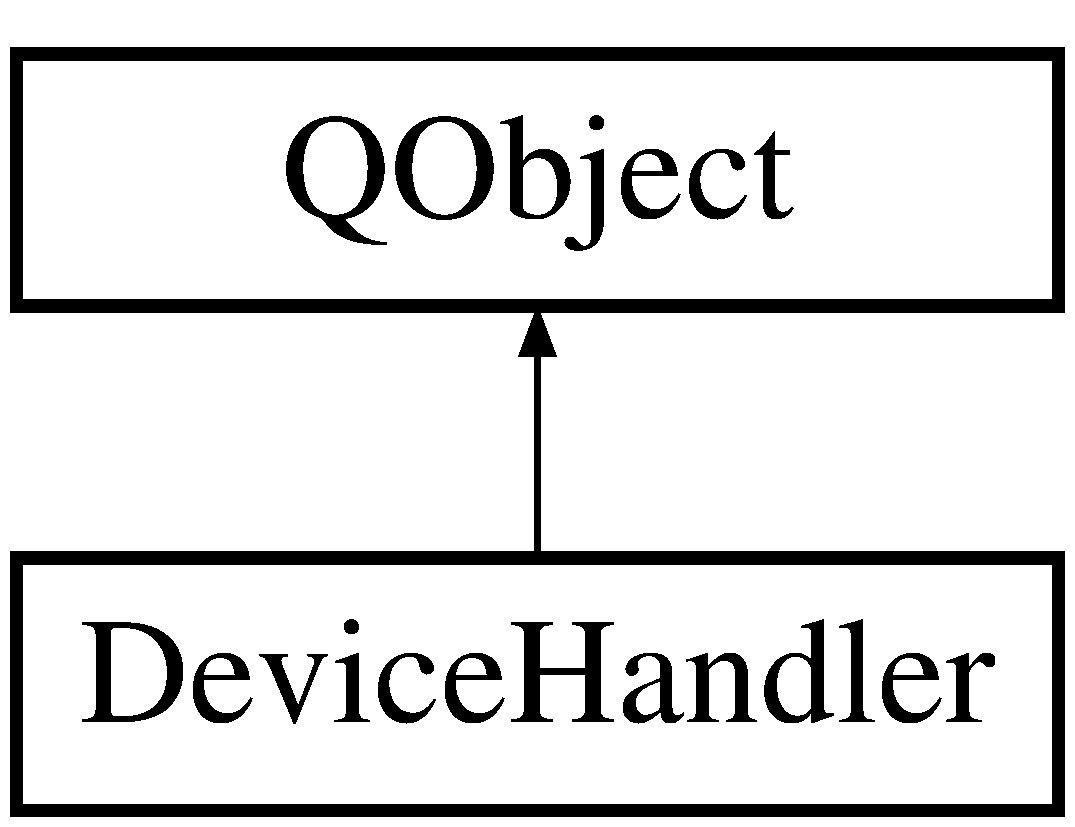
\includegraphics[height=2.604651cm]{class_device_handler}
\end{center}
\end{figure}
\subsection*{Public Member Functions}
\begin{DoxyCompactItemize}
\item 
\mbox{\Hypertarget{class_device_handler_ab16ab4b34974a0f4047851210e4825a7}\label{class_device_handler_ab16ab4b34974a0f4047851210e4825a7}} 
{\bfseries Device\+Handler} (\hyperlink{_global_defs_8h_ad17679fac69973be9b3a2787a60d7722}{Device\+Class\+Enum} class\+Code, Q\+Object $\ast$parent=0)
\item 
\mbox{\Hypertarget{class_device_handler_a117ebae8784b275f5dfc8bcf0b32f662}\label{class_device_handler_a117ebae8784b275f5dfc8bcf0b32f662}} 
\hyperlink{_global_defs_8h_ad17679fac69973be9b3a2787a60d7722}{Device\+Class\+Enum} {\bfseries get\+Class\+Code} (void) const
\end{DoxyCompactItemize}


The documentation for this class was generated from the following files\+:\begin{DoxyCompactItemize}
\item 
L\+C\+S\+Server/Device\+Handler.\+h\item 
L\+C\+S\+Server/Device\+Handler.\+cpp\end{DoxyCompactItemize}

\hypertarget{class_device_manager}{}\section{Device\+Manager Class Reference}
\label{class_device_manager}\index{Device\+Manager@{Device\+Manager}}
Inheritance diagram for Device\+Manager\+:\begin{figure}[H]
\begin{center}
\leavevmode
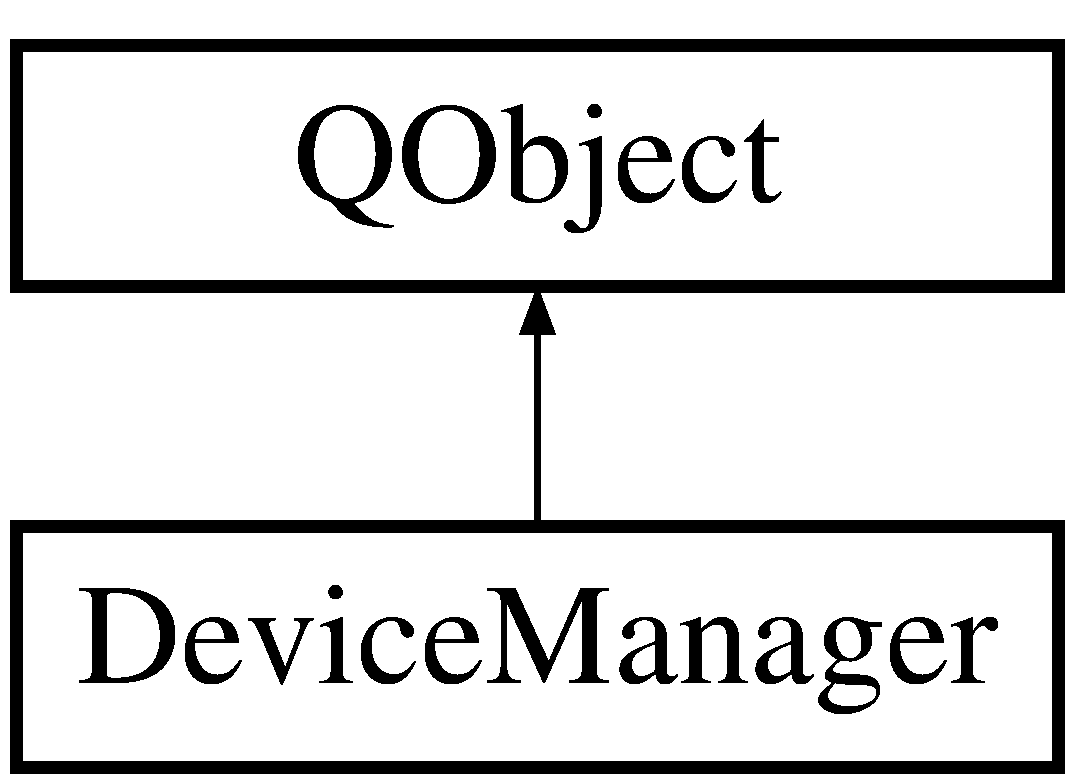
\includegraphics[height=2.000000cm]{class_device_manager}
\end{center}
\end{figure}
\subsection*{Public Slots}
\begin{DoxyCompactItemize}
\item 
\mbox{\Hypertarget{class_device_manager_a693a3a80d7cefeaabbc29fd8695f9e1a}\label{class_device_manager_a693a3a80d7cefeaabbc29fd8695f9e1a}} 
\hyperlink{class_device_handler}{Device\+Handler} $\ast$ {\bfseries get\+Handler} (\hyperlink{_global_defs_8h_ad17679fac69973be9b3a2787a60d7722}{Device\+Class\+Enum} class\+Code) const
\item 
\mbox{\Hypertarget{class_device_manager_a037575d38c8aa473d57de2950e0daa18}\label{class_device_manager_a037575d38c8aa473d57de2950e0daa18}} 
void {\bfseries set\+Device\+Status} (int device\+ID, int status)
\item 
\mbox{\Hypertarget{class_device_manager_aa231eea3b24b3418482506be4b7d02ef}\label{class_device_manager_aa231eea3b24b3418482506be4b7d02ef}} 
void {\bfseries new\+U\+D\+P\+Message} (const \hyperlink{class_u_d_p_message}{U\+D\+P\+Message} \&message)
\end{DoxyCompactItemize}
\subsection*{Signals}
\begin{DoxyCompactItemize}
\item 
\mbox{\Hypertarget{class_device_manager_aa96a714f5d7b0a43c5b37622df5f4800}\label{class_device_manager_aa96a714f5d7b0a43c5b37622df5f4800}} 
void {\bfseries device\+Status\+Changed} (int device\+ID, int status)
\item 
\mbox{\Hypertarget{class_device_manager_a2b8369554a4720f18d7ab3aef8a847ec}\label{class_device_manager_a2b8369554a4720f18d7ab3aef8a847ec}} 
void {\bfseries send\+Notification\+Message} (const Q\+String \&uri, const Q\+Json\+Object \&obj)
\end{DoxyCompactItemize}
\subsection*{Public Member Functions}
\begin{DoxyCompactItemize}
\item 
\mbox{\Hypertarget{class_device_manager_af96ef91b388d9f62165268fa6e388e0c}\label{class_device_manager_af96ef91b388d9f62165268fa6e388e0c}} 
int {\bfseries get\+Device\+Status} (int device\+ID)
\item 
\mbox{\Hypertarget{class_device_manager_a982b59b42355c617b548d1fb7b766664}\label{class_device_manager_a982b59b42355c617b548d1fb7b766664}} 
int {\bfseries get\+Device\+Count} (void) const
\item 
\mbox{\Hypertarget{class_device_manager_a1d41fc384c0a2d87192506636440c3d1}\label{class_device_manager_a1d41fc384c0a2d87192506636440c3d1}} 
int {\bfseries get\+Device\+ID} (int index) const
\end{DoxyCompactItemize}
\subsection*{Static Public Member Functions}
\begin{DoxyCompactItemize}
\item 
\mbox{\Hypertarget{class_device_manager_acce31b85af330247c7d41f278209b265}\label{class_device_manager_acce31b85af330247c7d41f278209b265}} 
static \hyperlink{class_device_manager}{Device\+Manager} $\ast$ {\bfseries instance} (void)
\end{DoxyCompactItemize}
\subsection*{Protected Member Functions}
\begin{DoxyCompactItemize}
\item 
\mbox{\Hypertarget{class_device_manager_ae1ff953a62461bf8326c73fdb509d50e}\label{class_device_manager_ae1ff953a62461bf8326c73fdb509d50e}} 
void {\bfseries add\+Device\+Handler} (\hyperlink{_global_defs_8h_ad17679fac69973be9b3a2787a60d7722}{Device\+Class\+Enum} class\+Code, \hyperlink{class_device_handler}{Device\+Handler} $\ast$handler)
\item 
\mbox{\Hypertarget{class_device_manager_a37e887fcdbd35963fbfe00006202807f}\label{class_device_manager_a37e887fcdbd35963fbfe00006202807f}} 
void {\bfseries remove\+Device\+Handler} (\hyperlink{_global_defs_8h_ad17679fac69973be9b3a2787a60d7722}{Device\+Class\+Enum} class\+Code)
\end{DoxyCompactItemize}
\subsection*{Friends}
\begin{DoxyCompactItemize}
\item 
\mbox{\Hypertarget{class_device_manager_a2fd82f6ba5a09bc3061ec8fe2ce5098b}\label{class_device_manager_a2fd82f6ba5a09bc3061ec8fe2ce5098b}} 
class {\bfseries Device\+Handler}
\end{DoxyCompactItemize}


The documentation for this class was generated from the following files\+:\begin{DoxyCompactItemize}
\item 
L\+C\+S\+Server/Device\+Manager.\+h\item 
L\+C\+S\+Server/Device\+Manager.\+cpp\end{DoxyCompactItemize}

\hypertarget{class_device_status}{}\section{Device\+Status Class Reference}
\label{class_device_status}\index{Device\+Status@{Device\+Status}}
\subsection*{Public Member Functions}
\begin{DoxyCompactItemize}
\item 
\mbox{\Hypertarget{class_device_status_a64d53902c3af6f9c0a3c1eb8c2f9ac69}\label{class_device_status_a64d53902c3af6f9c0a3c1eb8c2f9ac69}} 
{\bfseries Device\+Status} (bool locked, int status, const Q\+Date\+Time \&date\+Time)
\item 
\mbox{\Hypertarget{class_device_status_a79f1d523ceb98afe28170daf26b781a3}\label{class_device_status_a79f1d523ceb98afe28170daf26b781a3}} 
{\bfseries Device\+Status} (const \hyperlink{class_device_status}{Device\+Status} \&other)
\item 
\mbox{\Hypertarget{class_device_status_ae822d2aff82fe04ab32d037e44dd01fb}\label{class_device_status_ae822d2aff82fe04ab32d037e44dd01fb}} 
void {\bfseries operator=} (const \hyperlink{class_device_status}{Device\+Status} \&other)
\item 
\mbox{\Hypertarget{class_device_status_a0bd9c473925b1ebab816df6b96078a43}\label{class_device_status_a0bd9c473925b1ebab816df6b96078a43}} 
int {\bfseries get\+Current\+Status} (void) const
\item 
\mbox{\Hypertarget{class_device_status_ae4f58c4b39533c3965d85bef2163c054}\label{class_device_status_ae4f58c4b39533c3965d85bef2163c054}} 
void {\bfseries set\+Current\+Status} (int value)
\item 
\mbox{\Hypertarget{class_device_status_a0cf30022d1b60999a58fbfb84307aa72}\label{class_device_status_a0cf30022d1b60999a58fbfb84307aa72}} 
Q\+Date\+Time {\bfseries get\+Status\+Date\+Time} (void) const
\item 
\mbox{\Hypertarget{class_device_status_a788e3212b95a214e99eb90a7a0448726}\label{class_device_status_a788e3212b95a214e99eb90a7a0448726}} 
void {\bfseries set\+Status\+Date\+Time} (const Q\+Date\+Time \&value)
\item 
\mbox{\Hypertarget{class_device_status_a9ccab45320a1bf09c599bd2cdfd05257}\label{class_device_status_a9ccab45320a1bf09c599bd2cdfd05257}} 
bool {\bfseries get\+Locked} (void) const
\item 
\mbox{\Hypertarget{class_device_status_aeec173f78766305c666877983e75d957}\label{class_device_status_aeec173f78766305c666877983e75d957}} 
void {\bfseries set\+Locked} (bool value)
\end{DoxyCompactItemize}


The documentation for this class was generated from the following file\+:\begin{DoxyCompactItemize}
\item 
L\+C\+S\+Server/Device\+Manager.\+h\end{DoxyCompactItemize}

\hypertarget{class_entity_metadata}{}\section{Entity\+Metadata Class Reference}
\label{class_entity_metadata}\index{Entity\+Metadata@{Entity\+Metadata}}
Inheritance diagram for Entity\+Metadata\+:\begin{figure}[H]
\begin{center}
\leavevmode
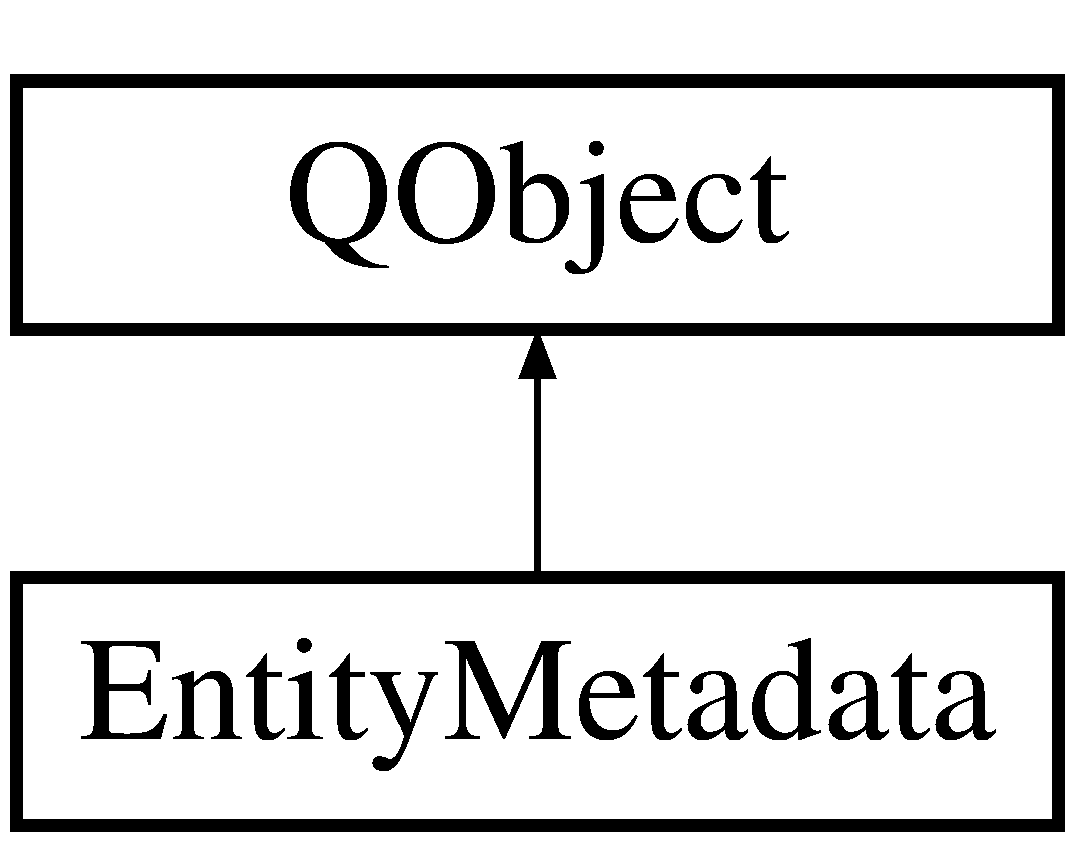
\includegraphics[height=2.000000cm]{class_entity_metadata}
\end{center}
\end{figure}
\subsection*{Public Slots}
\begin{DoxyCompactItemize}
\item 
\mbox{\Hypertarget{class_entity_metadata_ae1e3ddaa6d5e273e2a570c7dd8c4c67f}\label{class_entity_metadata_ae1e3ddaa6d5e273e2a570c7dd8c4c67f}} 
Q\+String {\bfseries get\+Table\+Name} (const Q\+String \&entity\+Name) const
\item 
\mbox{\Hypertarget{class_entity_metadata_a7001c5eaf5f4a32e3536cc218764de2b}\label{class_entity_metadata_a7001c5eaf5f4a32e3536cc218764de2b}} 
Q\+String {\bfseries get\+Key\+Field} (const Q\+String \&entity\+Name) const
\item 
\mbox{\Hypertarget{class_entity_metadata_aa22160232e36df2ee7ba52e29194cafb}\label{class_entity_metadata_aa22160232e36df2ee7ba52e29194cafb}} 
Q\+String {\bfseries get\+Table\+Field} (const Q\+String \&entity\+Name) const
\end{DoxyCompactItemize}
\subsection*{Public Member Functions}
\begin{DoxyCompactItemize}
\item 
\mbox{\Hypertarget{class_entity_metadata_a517cbc300798b6d9cdddb2d7d00c0e4e}\label{class_entity_metadata_a517cbc300798b6d9cdddb2d7d00c0e4e}} 
{\bfseries Entity\+Metadata} (Q\+Object $\ast$parent=N\+U\+LL)
\end{DoxyCompactItemize}
\subsection*{Static Public Member Functions}
\begin{DoxyCompactItemize}
\item 
\mbox{\Hypertarget{class_entity_metadata_a4aa1b5e44eea34614fcea132ecbd05ac}\label{class_entity_metadata_a4aa1b5e44eea34614fcea132ecbd05ac}} 
static \hyperlink{class_entity_metadata}{Entity\+Metadata} $\ast$ {\bfseries instance} (void)
\end{DoxyCompactItemize}


The documentation for this class was generated from the following files\+:\begin{DoxyCompactItemize}
\item 
L\+C\+S\+Server/Entity\+Metadata.\+h\item 
L\+C\+S\+Server/Entity\+Metadata.\+cpp\end{DoxyCompactItemize}

\hypertarget{class_handler_thread}{}\section{Handler\+Thread Class Reference}
\label{class_handler_thread}\index{Handler\+Thread@{Handler\+Thread}}
Inheritance diagram for Handler\+Thread\+:\begin{figure}[H]
\begin{center}
\leavevmode
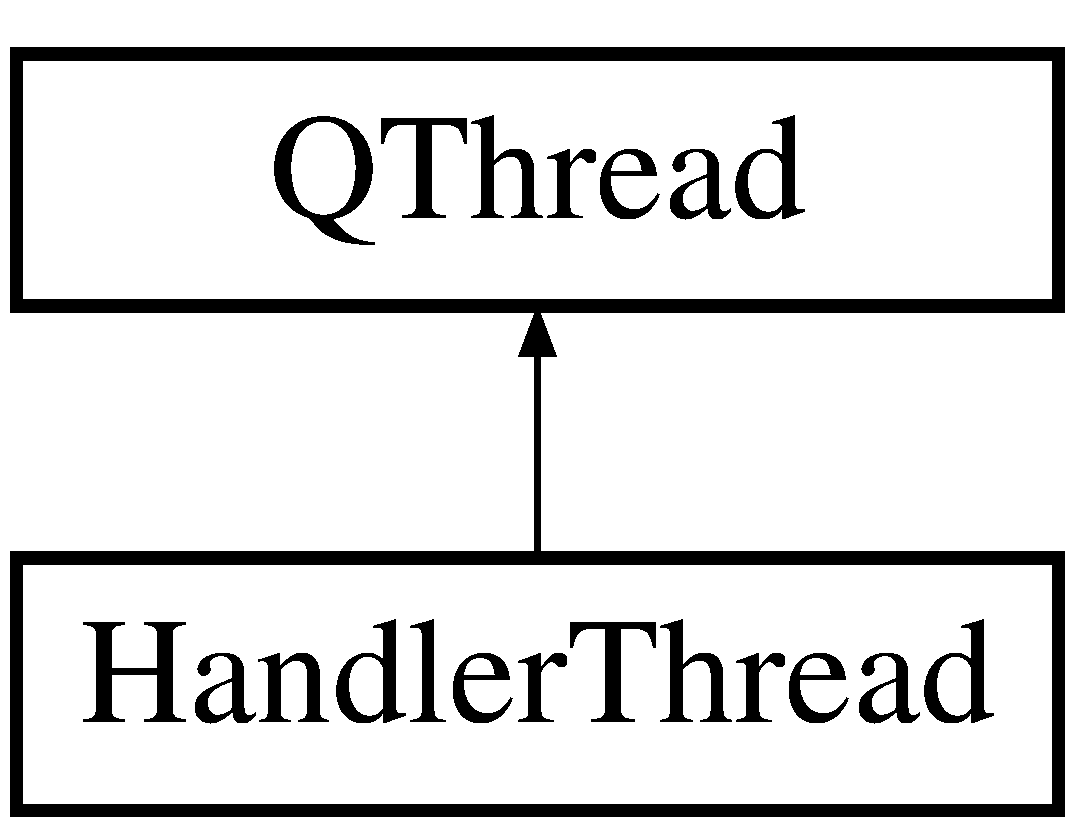
\includegraphics[height=2.000000cm]{class_handler_thread}
\end{center}
\end{figure}
\subsection*{Public Member Functions}
\begin{DoxyCompactItemize}
\item 
\mbox{\Hypertarget{class_handler_thread_a2425fd3ef03366b018c39cf6e1197383}\label{class_handler_thread_a2425fd3ef03366b018c39cf6e1197383}} 
bool {\bfseries called\+Ok} ()
\item 
\mbox{\Hypertarget{class_handler_thread_af6b14aa00f655a01d9d7f9f37e755a01}\label{class_handler_thread_af6b14aa00f655a01d9d7f9f37e755a01}} 
bool {\bfseries running\+As\+Console} ()
\end{DoxyCompactItemize}
\subsection*{Protected Member Functions}
\begin{DoxyCompactItemize}
\item 
\mbox{\Hypertarget{class_handler_thread_a1b8072811a6f79a18f332054d05d4a0d}\label{class_handler_thread_a1b8072811a6f79a18f332054d05d4a0d}} 
void {\bfseries run} ()
\end{DoxyCompactItemize}
\subsection*{Protected Attributes}
\begin{DoxyCompactItemize}
\item 
\mbox{\Hypertarget{class_handler_thread_ae939de0dcd9efdfbdda0bc8a67320241}\label{class_handler_thread_ae939de0dcd9efdfbdda0bc8a67320241}} 
bool {\bfseries success}
\item 
\mbox{\Hypertarget{class_handler_thread_a094154c070cd65f1cf971d022b6966eb}\label{class_handler_thread_a094154c070cd65f1cf971d022b6966eb}} 
bool {\bfseries console}
\end{DoxyCompactItemize}


The documentation for this class was generated from the following file\+:\begin{DoxyCompactItemize}
\item 
L\+C\+S\+Server/\+Qt\+Solutions\+Service/src/qtservice\+\_\+win.\+cpp\end{DoxyCompactItemize}

\hypertarget{union_i_p4_address_union}{}\section{I\+P4\+Address\+Union Union Reference}
\label{union_i_p4_address_union}\index{I\+P4\+Address\+Union@{I\+P4\+Address\+Union}}
\subsection*{Public Attributes}
\begin{DoxyCompactItemize}
\item 
\mbox{\Hypertarget{union_i_p4_address_union_abdbfed2541371505a7ea534a37f35cbe}\label{union_i_p4_address_union_abdbfed2541371505a7ea534a37f35cbe}} 
quint32 {\bfseries address32}
\item 
\mbox{\Hypertarget{union_i_p4_address_union_a97933d1b68d57bd37370816cb2f194ee}\label{union_i_p4_address_union_a97933d1b68d57bd37370816cb2f194ee}} 
quint8 {\bfseries bytes} \mbox{[}4\mbox{]}
\end{DoxyCompactItemize}


The documentation for this union was generated from the following file\+:\begin{DoxyCompactItemize}
\item 
L\+C\+S\+Server/Message\+Broadcaster.\+h\end{DoxyCompactItemize}

\hypertarget{class_message_broadcaster}{}\section{Message\+Broadcaster Class Reference}
\label{class_message_broadcaster}\index{Message\+Broadcaster@{Message\+Broadcaster}}
Inheritance diagram for Message\+Broadcaster\+:\begin{figure}[H]
\begin{center}
\leavevmode
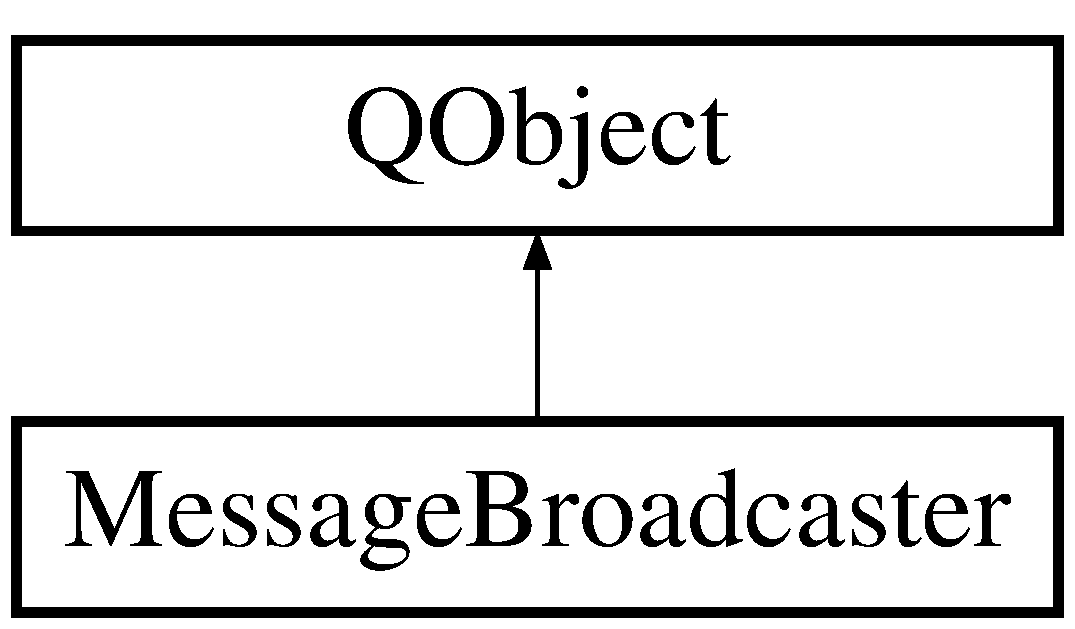
\includegraphics[height=2.000000cm]{class_message_broadcaster}
\end{center}
\end{figure}
\subsection*{Public Slots}
\begin{DoxyCompactItemize}
\item 
\mbox{\Hypertarget{class_message_broadcaster_a32dd162386ef2cf4414b7002d71ab660}\label{class_message_broadcaster_a32dd162386ef2cf4414b7002d71ab660}} 
void {\bfseries send\+Reset\+Notification\+List\+Command} (int serial\+Number)
\item 
\mbox{\Hypertarget{class_message_broadcaster_a84f20dff37d73c00f739de7f9e73c178}\label{class_message_broadcaster_a84f20dff37d73c00f739de7f9e73c178}} 
void {\bfseries send\+Reset\+Command} (int serial\+Number)
\item 
\mbox{\Hypertarget{class_message_broadcaster_ac18353484a67721b95ec1ea80f247549}\label{class_message_broadcaster_ac18353484a67721b95ec1ea80f247549}} 
void {\bfseries send\+Reset\+Config\+Command} (int serial\+Number)
\item 
\mbox{\Hypertarget{class_message_broadcaster_a2a6cfe9e14ba853d287b15d140ba31ce}\label{class_message_broadcaster_a2a6cfe9e14ba853d287b15d140ba31ce}} 
void {\bfseries send\+Reset\+Device\+Config\+Command} (int device\+ID)
\item 
\mbox{\Hypertarget{class_message_broadcaster_ac58cc1d5b6bd1211079cb74154cd2f0a}\label{class_message_broadcaster_ac58cc1d5b6bd1211079cb74154cd2f0a}} 
void {\bfseries send\+Lock\+Route\+Command} (int route\+ID, bool lock)
\item 
\mbox{\Hypertarget{class_message_broadcaster_ad5aaa609256cb4d94f966069d16ddcc0}\label{class_message_broadcaster_ad5aaa609256cb4d94f966069d16ddcc0}} 
void {\bfseries send\+Download\+Firmware} (int serial\+Number)
\item 
\mbox{\Hypertarget{class_message_broadcaster_a74aecd50e19ec44b1f594845675e4e68}\label{class_message_broadcaster_a74aecd50e19ec44b1f594845675e4e68}} 
void {\bfseries send\+Message} (int message\+ID, int serial\+Number, quint8 byte1, quint8 byte2=0, quint8 byte3=0, quint8 byte4=0, quint8 byte5=0)
\item 
\mbox{\Hypertarget{class_message_broadcaster_ad34fa164afe43eea0a114677590d6f01}\label{class_message_broadcaster_ad34fa164afe43eea0a114677590d6f01}} 
void {\bfseries send\+U\+D\+P\+Message} (const \hyperlink{class_u_d_p_message}{U\+D\+P\+Message} \&message)
\item 
\mbox{\Hypertarget{class_message_broadcaster_afe9d5032c449b68d33de82bd5b38d827}\label{class_message_broadcaster_afe9d5032c449b68d33de82bd5b38d827}} 
bool {\bfseries send\+U\+D\+P\+Message} (const \hyperlink{class_u_d_p_message}{U\+D\+P\+Message} \&message, const Q\+String \&address)
\item 
\mbox{\Hypertarget{class_message_broadcaster_a688f90812e544dde1795fde0d48674c2}\label{class_message_broadcaster_a688f90812e544dde1795fde0d48674c2}} 
void {\bfseries enable\+Heartbeat\+Messages} (bool value)
\end{DoxyCompactItemize}
\subsection*{Signals}
\begin{DoxyCompactItemize}
\item 
\mbox{\Hypertarget{class_message_broadcaster_a5fd9f33c5596dd29a34a280c828d5d69}\label{class_message_broadcaster_a5fd9f33c5596dd29a34a280c828d5d69}} 
void {\bfseries new\+Message} (const \hyperlink{class_u_d_p_message}{U\+D\+P\+Message} \&message)
\item 
\mbox{\Hypertarget{class_message_broadcaster_a7beb9f1957e0616a367a63af4515200b}\label{class_message_broadcaster_a7beb9f1957e0616a367a63af4515200b}} 
void {\bfseries new\+Raw\+U\+D\+P\+Message} (const Q\+String \&message)
\item 
\mbox{\Hypertarget{class_message_broadcaster_a7c20965394c805fbf3b4e9bcd26ea562}\label{class_message_broadcaster_a7c20965394c805fbf3b4e9bcd26ea562}} 
void {\bfseries controller\+Resetting} (long serial\+Number)
\end{DoxyCompactItemize}
\subsection*{Public Member Functions}
\begin{DoxyCompactItemize}
\item 
\mbox{\Hypertarget{class_message_broadcaster_aad0a58bca9ec48cb0b0b0bf4c724e7f8}\label{class_message_broadcaster_aad0a58bca9ec48cb0b0b0bf4c724e7f8}} 
void {\bfseries broadcast\+Message} (const Q\+String \&data)
\end{DoxyCompactItemize}
\subsection*{Static Public Member Functions}
\begin{DoxyCompactItemize}
\item 
\mbox{\Hypertarget{class_message_broadcaster_aff3184a82432cde75fcaa24b76c89904}\label{class_message_broadcaster_aff3184a82432cde75fcaa24b76c89904}} 
static \hyperlink{class_message_broadcaster}{Message\+Broadcaster} $\ast$ {\bfseries instance} ()
\item 
\mbox{\Hypertarget{class_message_broadcaster_a5a0a4b1fb88a50dfeacb5a2e46c1013b}\label{class_message_broadcaster_a5a0a4b1fb88a50dfeacb5a2e46c1013b}} 
static void {\bfseries set\+Run\+As\+Client} (bool value)
\end{DoxyCompactItemize}
\subsection*{Protected Slots}
\begin{DoxyCompactItemize}
\item 
\mbox{\Hypertarget{class_message_broadcaster_a699e964a4d64025b5d31387a7e1e4db9}\label{class_message_broadcaster_a699e964a4d64025b5d31387a7e1e4db9}} 
void {\bfseries process\+Pending\+Messages} (void)
\item 
\mbox{\Hypertarget{class_message_broadcaster_a2e51c2d01ad3b6849f7ea653b2ab0d76}\label{class_message_broadcaster_a2e51c2d01ad3b6849f7ea653b2ab0d76}} 
void {\bfseries process\+Udp\+Buffer} (const Q\+Host\+Address \&address)
\item 
\mbox{\Hypertarget{class_message_broadcaster_af4784fce7b71681f321bda9c953db63b}\label{class_message_broadcaster_af4784fce7b71681f321bda9c953db63b}} 
void {\bfseries send\+Heartbeat\+Slot} (const \hyperlink{class_u_d_p_message}{U\+D\+P\+Message} \&message)
\item 
\mbox{\Hypertarget{class_message_broadcaster_a9d7639d045a65534a99fcf7621681688}\label{class_message_broadcaster_a9d7639d045a65534a99fcf7621681688}} 
void {\bfseries heartbeat\+Timer\+Slot} (void)
\item 
\mbox{\Hypertarget{class_message_broadcaster_ae138b05340d5f3536668a674cdca0d01}\label{class_message_broadcaster_ae138b05340d5f3536668a674cdca0d01}} 
void {\bfseries send\+Keep\+Alive\+Message\+Slot} (void)
\item 
\mbox{\Hypertarget{class_message_broadcaster_a54843b46cff4ac2a53c5f25ecf428443}\label{class_message_broadcaster_a54843b46cff4ac2a53c5f25ecf428443}} 
void {\bfseries controller\+Restarting} (const \hyperlink{class_u_d_p_message}{U\+D\+P\+Message} \&message)
\end{DoxyCompactItemize}


The documentation for this class was generated from the following files\+:\begin{DoxyCompactItemize}
\item 
L\+C\+S\+Server/Message\+Broadcaster.\+h\item 
L\+C\+S\+Server/Message\+Broadcaster.\+cpp\end{DoxyCompactItemize}

\hypertarget{class_n_c_e_interface}{}\section{N\+C\+E\+Interface Class Reference}
\label{class_n_c_e_interface}\index{N\+C\+E\+Interface@{N\+C\+E\+Interface}}
Inheritance diagram for N\+C\+E\+Interface\+:\begin{figure}[H]
\begin{center}
\leavevmode
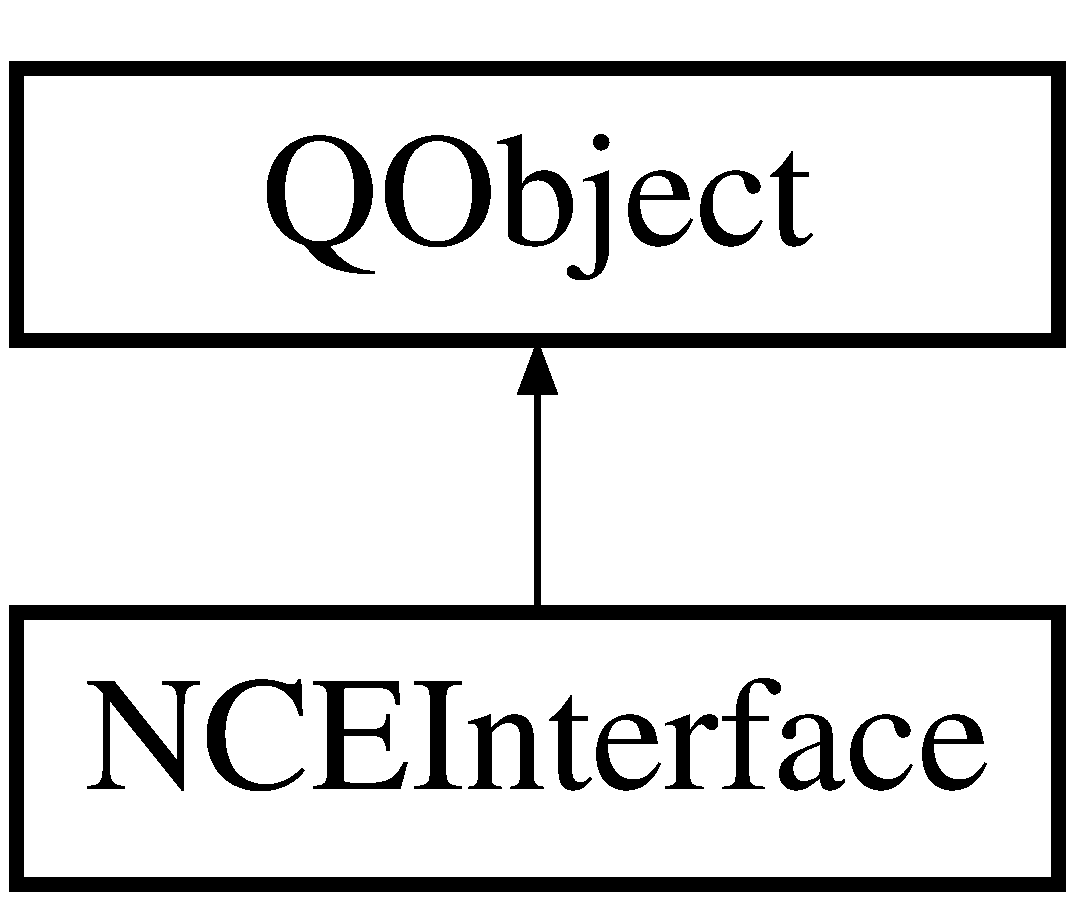
\includegraphics[height=2.000000cm]{class_n_c_e_interface}
\end{center}
\end{figure}
\subsection*{Public Slots}
\begin{DoxyCompactItemize}
\item 
\mbox{\Hypertarget{class_n_c_e_interface_a47932f97e62740e4734fc5a365462b96}\label{class_n_c_e_interface_a47932f97e62740e4734fc5a365462b96}} 
void {\bfseries new\+Message\+Slot} (const \hyperlink{class_n_c_e_message}{N\+C\+E\+Message} \&message)
\item 
\mbox{\Hypertarget{class_n_c_e_interface_a61db42f2bacec3b7f7a234bab9f11899}\label{class_n_c_e_interface_a61db42f2bacec3b7f7a234bab9f11899}} 
void {\bfseries route\+Status\+Changed} (int route\+ID, bool is\+Active)
\item 
\mbox{\Hypertarget{class_n_c_e_interface_a7f5bc3afb5eda7d5747ffec5d13bfdc5}\label{class_n_c_e_interface_a7f5bc3afb5eda7d5747ffec5d13bfdc5}} 
void {\bfseries device\+Status\+Changed} (int device\+ID, int status, bool locked)
\end{DoxyCompactItemize}
\subsection*{Signals}
\begin{DoxyCompactItemize}
\item 
\mbox{\Hypertarget{class_n_c_e_interface_a7bdaaf5c257df06fafd28579dd1fc594}\label{class_n_c_e_interface_a7bdaaf5c257df06fafd28579dd1fc594}} 
void {\bfseries send\+Message\+Signal} (const \hyperlink{class_n_c_e_message}{N\+C\+E\+Message} \&message)
\item 
\mbox{\Hypertarget{class_n_c_e_interface_aeaa6c5acc594a5a439b9d208cce220c9}\label{class_n_c_e_interface_aeaa6c5acc594a5a439b9d208cce220c9}} 
void {\bfseries buffer\+Initialized} (void)
\item 
\mbox{\Hypertarget{class_n_c_e_interface_a23b6a6c8d9b16d27c83ebaa7df0d762b}\label{class_n_c_e_interface_a23b6a6c8d9b16d27c83ebaa7df0d762b}} 
void {\bfseries buffer\+Data\+Changed} (quint8 byte, int block\+Index, int byte\+Index)
\end{DoxyCompactItemize}
\subsection*{Public Member Functions}
\begin{DoxyCompactItemize}
\item 
\mbox{\Hypertarget{class_n_c_e_interface_aec68e1a283ae5633dad5d750547f5e74}\label{class_n_c_e_interface_aec68e1a283ae5633dad5d750547f5e74}} 
{\bfseries N\+C\+E\+Interface} (Q\+Object $\ast$parent=0)
\item 
\mbox{\Hypertarget{class_n_c_e_interface_abf6f3aa621e46ab329033beef6c44a90}\label{class_n_c_e_interface_abf6f3aa621e46ab329033beef6c44a90}} 
void {\bfseries setup} (void)
\item 
\mbox{\Hypertarget{class_n_c_e_interface_aa419dd65501c979e936309983dffcb86}\label{class_n_c_e_interface_aa419dd65501c979e936309983dffcb86}} 
void {\bfseries post\+Message} (const \hyperlink{class_n_c_e_message}{N\+C\+E\+Message} \&message)
\item 
\mbox{\Hypertarget{class_n_c_e_interface_aff52e3e08e79219ee4b632a320136aa7}\label{class_n_c_e_interface_aff52e3e08e79219ee4b632a320136aa7}} 
void {\bfseries send\+Message} (const \hyperlink{class_n_c_e_message}{N\+C\+E\+Message} \&message)
\end{DoxyCompactItemize}
\subsection*{Static Public Member Functions}
\begin{DoxyCompactItemize}
\item 
\mbox{\Hypertarget{class_n_c_e_interface_aac13b43a007b971cdb5a7e488e80cb2b}\label{class_n_c_e_interface_aac13b43a007b971cdb5a7e488e80cb2b}} 
static \hyperlink{class_n_c_e_interface}{N\+C\+E\+Interface} $\ast$ {\bfseries instance} (void)
\end{DoxyCompactItemize}


The documentation for this class was generated from the following files\+:\begin{DoxyCompactItemize}
\item 
L\+C\+S\+Server/N\+C\+E\+Interface.\+h\item 
L\+C\+S\+Server/N\+C\+E\+Interface.\+cpp\end{DoxyCompactItemize}

\hypertarget{class_n_c_e_message}{}\section{N\+C\+E\+Message Class Reference}
\label{class_n_c_e_message}\index{N\+C\+E\+Message@{N\+C\+E\+Message}}
\subsection*{Public Member Functions}
\begin{DoxyCompactItemize}
\item 
\mbox{\Hypertarget{class_n_c_e_message_ad46a18e4089cd3dd87e9de8a93f07e8e}\label{class_n_c_e_message_ad46a18e4089cd3dd87e9de8a93f07e8e}} 
{\bfseries N\+C\+E\+Message} (int command)
\item 
\mbox{\Hypertarget{class_n_c_e_message_a8b2fbd7eeabd6a5e74d8ca93e2dfecee}\label{class_n_c_e_message_a8b2fbd7eeabd6a5e74d8ca93e2dfecee}} 
{\bfseries N\+C\+E\+Message} (const \hyperlink{class_n_c_e_message}{N\+C\+E\+Message} \&other)
\item 
\mbox{\Hypertarget{class_n_c_e_message_a5c97e5f6738035fb7e5c98ad8624ac35}\label{class_n_c_e_message_a5c97e5f6738035fb7e5c98ad8624ac35}} 
bool {\bfseries is\+Valid} (void) const
\item 
\mbox{\Hypertarget{class_n_c_e_message_ad79c0e32f821502c9e9a4343276913b3}\label{class_n_c_e_message_ad79c0e32f821502c9e9a4343276913b3}} 
\hyperlink{class_n_c_e_message}{N\+C\+E\+Message} \& {\bfseries operator=} (const \hyperlink{class_n_c_e_message}{N\+C\+E\+Message} \&other)
\item 
\mbox{\Hypertarget{class_n_c_e_message_a5d39e79f97808b4b3657daa3dd848fa0}\label{class_n_c_e_message_a5d39e79f97808b4b3657daa3dd848fa0}} 
int {\bfseries get\+Command} (void) const
\item 
\mbox{\Hypertarget{class_n_c_e_message_a083087542d3d9632098ba3c2e6ff5dde}\label{class_n_c_e_message_a083087542d3d9632098ba3c2e6ff5dde}} 
Q\+Vector$<$ quint8 $>$ {\bfseries get\+Message\+Data} (void) const
\item 
\mbox{\Hypertarget{class_n_c_e_message_a73f4b0b13af1ee51c59c8b1fa90ca5c7}\label{class_n_c_e_message_a73f4b0b13af1ee51c59c8b1fa90ca5c7}} 
Q\+Vector$<$ quint8 $>$ {\bfseries get\+Result\+Data} (void) const
\item 
\mbox{\Hypertarget{class_n_c_e_message_a67f3a24b65151906d4f6d17af1e0242d}\label{class_n_c_e_message_a67f3a24b65151906d4f6d17af1e0242d}} 
void {\bfseries set\+Result\+Data} (const Q\+Vector$<$ quint8 $>$ \&value)
\item 
\mbox{\Hypertarget{class_n_c_e_message_adf38a01edd96b44fa818e09d9b6edfde}\label{class_n_c_e_message_adf38a01edd96b44fa818e09d9b6edfde}} 
void {\bfseries acc\+Decoder} (int number, bool normal)
\item 
\mbox{\Hypertarget{class_n_c_e_message_aa613a72881563a11c990a38ea3c28f61}\label{class_n_c_e_message_aa613a72881563a11c990a38ea3c28f61}} 
void {\bfseries acc\+Memory\+Read} (int address)
\item 
\mbox{\Hypertarget{class_n_c_e_message_ac0ef27fa39f603ba736e23d26802486f}\label{class_n_c_e_message_ac0ef27fa39f603ba736e23d26802486f}} 
void {\bfseries get\+Version} (void)
\item 
\mbox{\Hypertarget{class_n_c_e_message_a67590c53183a7846bf641e3109243cd3}\label{class_n_c_e_message_a67590c53183a7846bf641e3109243cd3}} 
int {\bfseries get\+Expected\+Size} (void) const
\end{DoxyCompactItemize}
\subsection*{Static Public Attributes}
\begin{DoxyCompactItemize}
\item 
\mbox{\Hypertarget{class_n_c_e_message_a8ef313ccd6c59b55d14c466865999c81}\label{class_n_c_e_message_a8ef313ccd6c59b55d14c466865999c81}} 
static const quint8 {\bfseries N\+O\+O\+P\+\_\+\+C\+MD} = 0x80
\item 
\mbox{\Hypertarget{class_n_c_e_message_a93a9ca65ec9f484274a92d589e9f688f}\label{class_n_c_e_message_a93a9ca65ec9f484274a92d589e9f688f}} 
static const quint8 {\bfseries A\+S\+S\+I\+G\+N\+\_\+\+C\+A\+B\+\_\+\+C\+MD} = 0x81
\item 
\mbox{\Hypertarget{class_n_c_e_message_af9bb9ad4db1b3623cbb346fd7e324991}\label{class_n_c_e_message_af9bb9ad4db1b3623cbb346fd7e324991}} 
static const quint8 {\bfseries R\+E\+A\+D\+\_\+\+C\+L\+O\+C\+K\+\_\+\+C\+MD} = 0x82
\item 
\mbox{\Hypertarget{class_n_c_e_message_ab0f451e3bf5b078f9c26f55e468b2e67}\label{class_n_c_e_message_ab0f451e3bf5b078f9c26f55e468b2e67}} 
static const quint8 {\bfseries S\+T\+O\+P\+\_\+\+C\+L\+O\+C\+K\+\_\+\+C\+MD} = 0x83
\item 
\mbox{\Hypertarget{class_n_c_e_message_a159c08d633927ac84282d09a41e1ad0d}\label{class_n_c_e_message_a159c08d633927ac84282d09a41e1ad0d}} 
static const quint8 {\bfseries S\+T\+A\+R\+T\+\_\+\+C\+L\+O\+C\+K\+\_\+\+C\+MD} = 0x84
\item 
\mbox{\Hypertarget{class_n_c_e_message_a7a0fd35d38156eca70a6f98855eb1cbc}\label{class_n_c_e_message_a7a0fd35d38156eca70a6f98855eb1cbc}} 
static const quint8 {\bfseries S\+E\+T\+\_\+\+C\+L\+O\+C\+K\+\_\+\+C\+MD} = 0x85
\item 
\mbox{\Hypertarget{class_n_c_e_message_a4d80eabc10732e8c027423fb7b58dddb}\label{class_n_c_e_message_a4d80eabc10732e8c027423fb7b58dddb}} 
static const quint8 {\bfseries C\+L\+O\+C\+K\+\_\+1224\+\_\+\+C\+MD} = 0x86
\item 
\mbox{\Hypertarget{class_n_c_e_message_a5ed9e5ed3e0ab472612186948c4337c3}\label{class_n_c_e_message_a5ed9e5ed3e0ab472612186948c4337c3}} 
static const quint8 {\bfseries C\+L\+O\+C\+K\+\_\+\+R\+A\+T\+I\+O\+\_\+\+C\+MD} = 0x87
\item 
\mbox{\Hypertarget{class_n_c_e_message_ae99776528295bc12b5183f9568b1bb63}\label{class_n_c_e_message_ae99776528295bc12b5183f9568b1bb63}} 
static const quint8 {\bfseries D\+E\+Q\+U\+E\+U\+E\+\_\+\+C\+MD} = 0x88
\item 
\mbox{\Hypertarget{class_n_c_e_message_a930ba131bfd79c452836a3b256f979c4}\label{class_n_c_e_message_a930ba131bfd79c452836a3b256f979c4}} 
static const quint8 {\bfseries E\+N\+A\+B\+L\+E\+\_\+\+T\+R\+A\+C\+K\+\_\+\+C\+MD} = 0x89
\item 
\mbox{\Hypertarget{class_n_c_e_message_aac1564079746b0fdf703a6f29cc4ad33}\label{class_n_c_e_message_aac1564079746b0fdf703a6f29cc4ad33}} 
static const quint8 {\bfseries R\+E\+A\+D\+\_\+\+A\+U\+I4\+\_\+\+C\+MD} = 0x8A
\item 
\mbox{\Hypertarget{class_n_c_e_message_ae38e9eb5b4ccf36a4004a0194a0f5bc0}\label{class_n_c_e_message_ae38e9eb5b4ccf36a4004a0194a0f5bc0}} 
static const quint8 {\bfseries D\+I\+S\+A\+B\+L\+E\+\_\+\+T\+R\+A\+C\+K\+\_\+\+C\+MD} = 0x89
\item 
\mbox{\Hypertarget{class_n_c_e_message_ab0bc8e607d4d53ec2e9c08dc8d72b988}\label{class_n_c_e_message_ab0bc8e607d4d53ec2e9c08dc8d72b988}} 
static const quint8 {\bfseries D\+U\+M\+M\+Y\+\_\+\+C\+MD} = 0x8C
\item 
\mbox{\Hypertarget{class_n_c_e_message_aa1743907c9945e2efb7241b32639f67c}\label{class_n_c_e_message_aa1743907c9945e2efb7241b32639f67c}} 
static const quint8 {\bfseries S\+P\+E\+E\+D\+\_\+\+M\+O\+D\+E\+\_\+\+C\+MD} = 0x8D
\item 
\mbox{\Hypertarget{class_n_c_e_message_ac3c325b65d98f36b5a90d592074aff45}\label{class_n_c_e_message_ac3c325b65d98f36b5a90d592074aff45}} 
static const quint8 {\bfseries W\+R\+I\+T\+E\+\_\+\+N\+\_\+\+C\+MD} = 0x8E
\item 
\mbox{\Hypertarget{class_n_c_e_message_ad26e49bc959198a70f6cc3eeed97b585}\label{class_n_c_e_message_ad26e49bc959198a70f6cc3eeed97b585}} 
static const quint8 {\bfseries R\+E\+A\+D16\+\_\+\+C\+MD} = 0x8F
\item 
\mbox{\Hypertarget{class_n_c_e_message_a3f1f3bf89bd95e37752c75987a12b86a}\label{class_n_c_e_message_a3f1f3bf89bd95e37752c75987a12b86a}} 
static const quint8 {\bfseries D\+I\+S\+P\+L\+A\+Y3\+\_\+\+C\+MD} = 0x90
\item 
\mbox{\Hypertarget{class_n_c_e_message_ab6dac7fb6bd03c70fe7137c9676d3e87}\label{class_n_c_e_message_ab6dac7fb6bd03c70fe7137c9676d3e87}} 
static const quint8 {\bfseries D\+I\+S\+P\+L\+A\+Y4\+\_\+\+C\+MD} = 0x91
\item 
\mbox{\Hypertarget{class_n_c_e_message_a6f6bf1dd8c806daeded6067daa98a7a5}\label{class_n_c_e_message_a6f6bf1dd8c806daeded6067daa98a7a5}} 
static const quint8 {\bfseries D\+I\+S\+P\+L\+A\+Y2\+\_\+\+C\+MD} = 0x92
\item 
\mbox{\Hypertarget{class_n_c_e_message_a6c43dadbff52e1e3fb6479e61c66e4c9}\label{class_n_c_e_message_a6c43dadbff52e1e3fb6479e61c66e4c9}} 
static const quint8 {\bfseries Q\+U\+E\+U\+E3\+\_\+\+T\+M\+P\+\_\+\+C\+MD} = 0x93
\item 
\mbox{\Hypertarget{class_n_c_e_message_a2ff53743ba857c2c553826c3957f6b5b}\label{class_n_c_e_message_a2ff53743ba857c2c553826c3957f6b5b}} 
static const quint8 {\bfseries Q\+U\+E\+U\+E4\+\_\+\+T\+M\+P\+\_\+\+C\+MD} = 0x94
\item 
\mbox{\Hypertarget{class_n_c_e_message_ac0ea933cb703bcf2cecb6b27f1cc7cb1}\label{class_n_c_e_message_ac0ea933cb703bcf2cecb6b27f1cc7cb1}} 
static const quint8 {\bfseries Q\+U\+E\+U\+E5\+\_\+\+T\+M\+P\+\_\+\+C\+MD} = 0x95
\item 
\mbox{\Hypertarget{class_n_c_e_message_a6999178dbc500063b49b8aaf73002463}\label{class_n_c_e_message_a6999178dbc500063b49b8aaf73002463}} 
static const quint8 {\bfseries Q\+U\+E\+U\+E6\+\_\+\+T\+M\+P\+\_\+\+C\+MD} = 0x96
\item 
\mbox{\Hypertarget{class_n_c_e_message_a98b59cb78ec56c4364022fe48249d94d}\label{class_n_c_e_message_a98b59cb78ec56c4364022fe48249d94d}} 
static const quint8 {\bfseries W\+R\+I\+T\+E1\+\_\+\+C\+MD} = 0x97
\item 
\mbox{\Hypertarget{class_n_c_e_message_a7445ba7da027255122119e7ebb37e555}\label{class_n_c_e_message_a7445ba7da027255122119e7ebb37e555}} 
static const quint8 {\bfseries W\+R\+I\+T\+E2\+\_\+\+C\+MD} = 0x98
\item 
\mbox{\Hypertarget{class_n_c_e_message_aa225fee33656d6aadb3b8433d6dc99b0}\label{class_n_c_e_message_aa225fee33656d6aadb3b8433d6dc99b0}} 
static const quint8 {\bfseries W\+R\+I\+T\+E4\+\_\+\+C\+MD} = 0x99
\item 
\mbox{\Hypertarget{class_n_c_e_message_a695185072db8e9ffb5e3848797b95279}\label{class_n_c_e_message_a695185072db8e9ffb5e3848797b95279}} 
static const quint8 {\bfseries W\+R\+I\+T\+E8\+\_\+\+C\+MD} = 0x9A
\item 
\mbox{\Hypertarget{class_n_c_e_message_a25796c4fe42b55087a5b140eb9c26072}\label{class_n_c_e_message_a25796c4fe42b55087a5b140eb9c26072}} 
static const quint8 {\bfseries R\+E\+A\+D\+\_\+\+A\+U\+I2\+\_\+\+C\+MD} = 0x9B
\item 
\mbox{\Hypertarget{class_n_c_e_message_aab64ec8de81639f0b67d1dae3ce8d420}\label{class_n_c_e_message_aab64ec8de81639f0b67d1dae3ce8d420}} 
static const quint8 {\bfseries M\+A\+C\+R\+O\+\_\+\+C\+MD} = 0x9C
\item 
\mbox{\Hypertarget{class_n_c_e_message_a594998390008c1d5c80352855a7f8e56}\label{class_n_c_e_message_a594998390008c1d5c80352855a7f8e56}} 
static const quint8 {\bfseries R\+E\+A\+D1\+\_\+\+C\+MD} = 0x9D
\item 
\mbox{\Hypertarget{class_n_c_e_message_ad2acc190cdafcb808efa5b2afa1bf8c2}\label{class_n_c_e_message_ad2acc190cdafcb808efa5b2afa1bf8c2}} 
static const quint8 {\bfseries P\+G\+M\+\_\+\+T\+R\+K\+\_\+\+O\+N\+\_\+\+C\+MD} = 0x9E
\item 
\mbox{\Hypertarget{class_n_c_e_message_a990840e409d105e7fbbd78b7f8a248c9}\label{class_n_c_e_message_a990840e409d105e7fbbd78b7f8a248c9}} 
static const quint8 {\bfseries P\+G\+M\+\_\+\+T\+R\+K\+\_\+\+O\+F\+F\+\_\+\+C\+MD} = 0x9F
\item 
\mbox{\Hypertarget{class_n_c_e_message_a2f8eaaf76bf8f3d78cbb2938c3dc6ed8}\label{class_n_c_e_message_a2f8eaaf76bf8f3d78cbb2938c3dc6ed8}} 
static const quint8 {\bfseries P\+G\+M\+\_\+\+P\+A\+G\+E\+\_\+\+W\+R\+I\+T\+E\+\_\+\+C\+MD} = 0x\+A0
\item 
\mbox{\Hypertarget{class_n_c_e_message_a80622e5a4f69811d9a5c69e58bbafbe2}\label{class_n_c_e_message_a80622e5a4f69811d9a5c69e58bbafbe2}} 
static const quint8 {\bfseries P\+G\+M\+\_\+\+P\+A\+G\+E\+\_\+\+R\+E\+A\+D\+\_\+\+C\+MD} = 0x\+A1
\item 
\mbox{\Hypertarget{class_n_c_e_message_a81400194ed1beabafeeb35d1943c1798}\label{class_n_c_e_message_a81400194ed1beabafeeb35d1943c1798}} 
static const quint8 {\bfseries L\+O\+C\+O\+\_\+\+C\+MD} = 0x\+A2
\item 
\mbox{\Hypertarget{class_n_c_e_message_a9950ee811a7d3230ce6364db2374503f}\label{class_n_c_e_message_a9950ee811a7d3230ce6364db2374503f}} 
static const quint8 {\bfseries Q\+U\+E\+U\+E3\+\_\+\+T\+R\+K\+\_\+\+C\+MD} = 0x\+A3
\item 
\mbox{\Hypertarget{class_n_c_e_message_ae834a6cb12f4fece3af6cbddc7b22839}\label{class_n_c_e_message_ae834a6cb12f4fece3af6cbddc7b22839}} 
static const quint8 {\bfseries Q\+U\+E\+U\+E4\+\_\+\+T\+R\+K\+\_\+\+C\+MD} = 0x\+A4
\item 
\mbox{\Hypertarget{class_n_c_e_message_ad949e543d8fe1d2aeb398933499546f6}\label{class_n_c_e_message_ad949e543d8fe1d2aeb398933499546f6}} 
static const quint8 {\bfseries Q\+U\+E\+U\+E5\+\_\+\+T\+R\+K\+\_\+\+C\+MD} = 0x\+A5
\item 
\mbox{\Hypertarget{class_n_c_e_message_a5e4b6bc8e5d3f399ed87d0cf0c744d38}\label{class_n_c_e_message_a5e4b6bc8e5d3f399ed87d0cf0c744d38}} 
static const quint8 {\bfseries P\+G\+M\+\_\+\+R\+E\+G\+\_\+\+W\+R\+I\+T\+E\+\_\+\+C\+MD} = 0x\+A6
\item 
\mbox{\Hypertarget{class_n_c_e_message_a52b03a0b475a58e4e2b93632cee45cf6}\label{class_n_c_e_message_a52b03a0b475a58e4e2b93632cee45cf6}} 
static const quint8 {\bfseries P\+G\+M\+\_\+\+R\+E\+G\+\_\+\+R\+E\+A\+D\+\_\+\+C\+MD} = 0x\+A7
\item 
\mbox{\Hypertarget{class_n_c_e_message_afb8794c356aef459e263c2bbc44ba58d}\label{class_n_c_e_message_afb8794c356aef459e263c2bbc44ba58d}} 
static const quint8 {\bfseries P\+G\+M\+\_\+\+D\+I\+R\+\_\+\+W\+R\+I\+T\+E\+\_\+\+C\+MD} = 0x\+A8
\item 
\mbox{\Hypertarget{class_n_c_e_message_aab21f0c057cfe98b4d1879b7a7e286bb}\label{class_n_c_e_message_aab21f0c057cfe98b4d1879b7a7e286bb}} 
static const quint8 {\bfseries P\+G\+M\+\_\+\+D\+I\+R\+\_\+\+R\+E\+A\+D\+\_\+\+C\+MD} = 0x\+A9
\item 
\mbox{\Hypertarget{class_n_c_e_message_af50c51c7592d83b8e2c4e19449b4ebf3}\label{class_n_c_e_message_af50c51c7592d83b8e2c4e19449b4ebf3}} 
static const quint8 {\bfseries S\+W\+\_\+\+R\+E\+V\+\_\+\+C\+MD} = 0x\+AA
\item 
\mbox{\Hypertarget{class_n_c_e_message_a0c8f36e762ccfa9642c564a2df7d4dfd}\label{class_n_c_e_message_a0c8f36e762ccfa9642c564a2df7d4dfd}} 
static const quint8 {\bfseries R\+E\+S\+E\+T\+\_\+\+S\+O\+F\+T\+\_\+\+C\+MD} = 0x\+AB
\item 
\mbox{\Hypertarget{class_n_c_e_message_ac8b7f7c524044cf3ad89fd93f7318a14}\label{class_n_c_e_message_ac8b7f7c524044cf3ad89fd93f7318a14}} 
static const quint8 {\bfseries R\+E\+S\+E\+T\+\_\+\+H\+A\+R\+D\+\_\+\+C\+MD} = 0x\+AC
\item 
\mbox{\Hypertarget{class_n_c_e_message_a3babcd798c5a276e7154e087480af584}\label{class_n_c_e_message_a3babcd798c5a276e7154e087480af584}} 
static const quint8 {\bfseries A\+C\+C\+\_\+\+C\+MD} = 0x\+AD
\item 
\mbox{\Hypertarget{class_n_c_e_message_abb560a81f2bf0fa2810ffa4acb98d12c}\label{class_n_c_e_message_abb560a81f2bf0fa2810ffa4acb98d12c}} 
static const quint8 {\bfseries O\+P\+S\+\_\+\+P\+R\+O\+G\+\_\+\+L\+O\+C\+O\+\_\+\+C\+MD} = 0x\+AE
\item 
\mbox{\Hypertarget{class_n_c_e_message_a67cd90c3490e7cf82de4333c7d195f94}\label{class_n_c_e_message_a67cd90c3490e7cf82de4333c7d195f94}} 
static const quint8 {\bfseries O\+P\+S\+\_\+\+P\+R\+O\+G\+\_\+\+A\+C\+C\+Y\+\_\+\+C\+MD} = 0x\+AF
\item 
\mbox{\Hypertarget{class_n_c_e_message_af412792e9f0d444c1132a569c899cd41}\label{class_n_c_e_message_af412792e9f0d444c1132a569c899cd41}} 
static const quint8 {\bfseries F\+A\+C\+T\+O\+R\+Y\+\_\+\+T\+E\+S\+T\+\_\+\+C\+MD} = 0x\+B0
\item 
\mbox{\Hypertarget{class_n_c_e_message_a918dcc9275ac42f4c332b5daec3ade41}\label{class_n_c_e_message_a918dcc9275ac42f4c332b5daec3ade41}} 
static const quint8 {\bfseries U\+S\+B\+\_\+\+S\+E\+T\+\_\+\+C\+A\+B\+\_\+\+C\+MD} = 0x\+B1
\item 
\mbox{\Hypertarget{class_n_c_e_message_a2973406210a824247d98bf54308d748c}\label{class_n_c_e_message_a2973406210a824247d98bf54308d748c}} 
static const quint8 {\bfseries U\+S\+B\+\_\+\+M\+E\+M\+\_\+\+P\+O\+I\+N\+T\+E\+R\+\_\+\+C\+MD} = 0x\+B3
\item 
\mbox{\Hypertarget{class_n_c_e_message_a386295827d3e09e4a40b14b87663f730}\label{class_n_c_e_message_a386295827d3e09e4a40b14b87663f730}} 
static const quint8 {\bfseries U\+S\+B\+\_\+\+M\+E\+M\+\_\+\+W\+R\+I\+T\+E\+\_\+\+C\+MD} = 0x\+B4
\item 
\mbox{\Hypertarget{class_n_c_e_message_ae29408a74fb88d81353e2053a2bb9190}\label{class_n_c_e_message_ae29408a74fb88d81353e2053a2bb9190}} 
static const quint8 {\bfseries U\+S\+B\+\_\+\+M\+E\+M\+\_\+\+R\+E\+A\+D\+\_\+\+C\+MD} = 0x\+B5
\item 
\mbox{\Hypertarget{class_n_c_e_message_a5c49c45dca14707909b6bb57630e339c}\label{class_n_c_e_message_a5c49c45dca14707909b6bb57630e339c}} 
static const quint8 {\bfseries L\+O\+C\+O\+\_\+\+C\+M\+D\+\_\+\+R\+E\+V\+\_\+28\+S\+P\+E\+ED} = 0x01
\item 
\mbox{\Hypertarget{class_n_c_e_message_aeee6d4d067650d1c768d5a07a27dd212}\label{class_n_c_e_message_aeee6d4d067650d1c768d5a07a27dd212}} 
static const quint8 {\bfseries L\+O\+C\+O\+\_\+\+C\+M\+D\+\_\+\+F\+W\+D\+\_\+28\+S\+P\+E\+ED} = 0x02
\item 
\mbox{\Hypertarget{class_n_c_e_message_a7dfc478217a861484383524fb5b0f780}\label{class_n_c_e_message_a7dfc478217a861484383524fb5b0f780}} 
static const quint8 {\bfseries L\+O\+C\+O\+\_\+\+C\+M\+D\+\_\+\+R\+E\+V\+\_\+128\+S\+P\+E\+ED} = 0x03
\item 
\mbox{\Hypertarget{class_n_c_e_message_a65931244e5e08eab994637b84ee5e3f7}\label{class_n_c_e_message_a65931244e5e08eab994637b84ee5e3f7}} 
static const quint8 {\bfseries L\+O\+C\+O\+\_\+\+C\+M\+D\+\_\+\+F\+W\+D\+\_\+128\+S\+P\+E\+ED} = 0x04
\item 
\mbox{\Hypertarget{class_n_c_e_message_aa97de2743e72bfb35b7116fd6a481ebe}\label{class_n_c_e_message_aa97de2743e72bfb35b7116fd6a481ebe}} 
static const quint8 {\bfseries L\+O\+C\+O\+\_\+\+C\+M\+D\+\_\+\+R\+E\+V\+\_\+\+E\+S\+T\+OP} = 0x05
\item 
\mbox{\Hypertarget{class_n_c_e_message_a2b3510ece44ebd78e28ac145daabd12e}\label{class_n_c_e_message_a2b3510ece44ebd78e28ac145daabd12e}} 
static const quint8 {\bfseries L\+O\+C\+O\+\_\+\+C\+M\+D\+\_\+\+F\+W\+D\+\_\+\+E\+S\+T\+OP} = 0x06
\item 
\mbox{\Hypertarget{class_n_c_e_message_a4d8d329678f7d61c4c4192021209b593}\label{class_n_c_e_message_a4d8d329678f7d61c4c4192021209b593}} 
static const quint8 {\bfseries L\+O\+C\+O\+\_\+\+C\+M\+D\+\_\+\+F\+G1} = 0x07
\item 
\mbox{\Hypertarget{class_n_c_e_message_ac2108206495b2f84392a3114cc517943}\label{class_n_c_e_message_ac2108206495b2f84392a3114cc517943}} 
static const quint8 {\bfseries L\+O\+C\+O\+\_\+\+C\+M\+D\+\_\+\+F\+G2} = 0x08
\item 
\mbox{\Hypertarget{class_n_c_e_message_afad6eddcfce7784c1fa185f88ef551c3}\label{class_n_c_e_message_afad6eddcfce7784c1fa185f88ef551c3}} 
static const quint8 {\bfseries L\+O\+C\+O\+\_\+\+C\+M\+D\+\_\+\+F\+G3} = 0x09
\item 
\mbox{\Hypertarget{class_n_c_e_message_a193b6567f87e9b5f7418359b481d8703}\label{class_n_c_e_message_a193b6567f87e9b5f7418359b481d8703}} 
static const quint8 {\bfseries L\+O\+C\+O\+\_\+\+C\+M\+D\+\_\+\+F\+G4} = 0x15
\item 
\mbox{\Hypertarget{class_n_c_e_message_adf1edd3a38457c80fa48d8db5caf59da}\label{class_n_c_e_message_adf1edd3a38457c80fa48d8db5caf59da}} 
static const quint8 {\bfseries L\+O\+C\+O\+\_\+\+C\+M\+D\+\_\+\+F\+G5} = 0x16
\item 
\mbox{\Hypertarget{class_n_c_e_message_a1d86984708df5f5a320bd75b7e92d6fa}\label{class_n_c_e_message_a1d86984708df5f5a320bd75b7e92d6fa}} 
static const quint8 {\bfseries L\+O\+C\+O\+\_\+\+C\+M\+D\+\_\+\+R\+E\+V\+\_\+\+C\+O\+N\+S\+I\+S\+T\+\_\+\+L\+E\+AD} = 0x0A
\item 
\mbox{\Hypertarget{class_n_c_e_message_aacda7cc187a0b7e87623f83f74406904}\label{class_n_c_e_message_aacda7cc187a0b7e87623f83f74406904}} 
static const quint8 {\bfseries L\+O\+C\+O\+\_\+\+C\+M\+D\+\_\+\+F\+W\+D\+\_\+\+C\+O\+N\+S\+I\+S\+T\+\_\+\+L\+E\+AD} = 0x0B
\item 
\mbox{\Hypertarget{class_n_c_e_message_a3f36ec6795b300a2d0e32f9e43b23c2a}\label{class_n_c_e_message_a3f36ec6795b300a2d0e32f9e43b23c2a}} 
static const quint8 {\bfseries L\+O\+C\+O\+\_\+\+C\+M\+D\+\_\+\+R\+E\+V\+\_\+\+C\+O\+N\+S\+I\+S\+T\+\_\+\+R\+E\+AR} = 0x0C
\item 
\mbox{\Hypertarget{class_n_c_e_message_a01f488b90880e9432fab6400baed33d2}\label{class_n_c_e_message_a01f488b90880e9432fab6400baed33d2}} 
static const quint8 {\bfseries L\+O\+C\+O\+\_\+\+C\+M\+D\+\_\+\+F\+W\+D\+\_\+\+C\+O\+N\+S\+I\+S\+T\+\_\+\+R\+E\+AR} = 0x0D
\item 
\mbox{\Hypertarget{class_n_c_e_message_a55a0d0cf71838cbee94b9afcc6de9195}\label{class_n_c_e_message_a55a0d0cf71838cbee94b9afcc6de9195}} 
static const quint8 {\bfseries L\+O\+C\+O\+\_\+\+C\+M\+D\+\_\+\+R\+E\+V\+\_\+\+C\+O\+N\+S\+I\+S\+T\+\_\+\+M\+ID} = 0x0E
\item 
\mbox{\Hypertarget{class_n_c_e_message_af9d3309874e55aeaed14a66e7e5a5386}\label{class_n_c_e_message_af9d3309874e55aeaed14a66e7e5a5386}} 
static const quint8 {\bfseries L\+O\+C\+O\+\_\+\+C\+M\+D\+\_\+\+F\+W\+D\+\_\+\+C\+O\+N\+S\+I\+S\+T\+\_\+\+M\+ID} = 0x0F
\item 
\mbox{\Hypertarget{class_n_c_e_message_a7ae479c7e0f82a7aff2ca7be083f4cc3}\label{class_n_c_e_message_a7ae479c7e0f82a7aff2ca7be083f4cc3}} 
static const quint8 {\bfseries L\+O\+C\+O\+\_\+\+C\+M\+D\+\_\+\+D\+E\+L\+E\+T\+E\+\_\+\+L\+O\+C\+O\+\_\+\+C\+O\+N\+S\+I\+ST} = 0x10
\item 
\mbox{\Hypertarget{class_n_c_e_message_a89a165925842aa1151f0c0f0a98e6b24}\label{class_n_c_e_message_a89a165925842aa1151f0c0f0a98e6b24}} 
static const quint8 {\bfseries L\+O\+C\+O\+\_\+\+C\+M\+D\+\_\+\+K\+I\+L\+L\+\_\+\+C\+O\+N\+S\+I\+ST} = 0x11
\end{DoxyCompactItemize}


The documentation for this class was generated from the following files\+:\begin{DoxyCompactItemize}
\item 
L\+C\+S\+Server/N\+C\+E\+Message.\+h\item 
L\+C\+S\+Server/N\+C\+E\+Message.\+cpp\end{DoxyCompactItemize}

\hypertarget{class_notification_server}{}\section{Notification\+Server Class Reference}
\label{class_notification_server}\index{Notification\+Server@{Notification\+Server}}
Inheritance diagram for Notification\+Server\+:\begin{figure}[H]
\begin{center}
\leavevmode
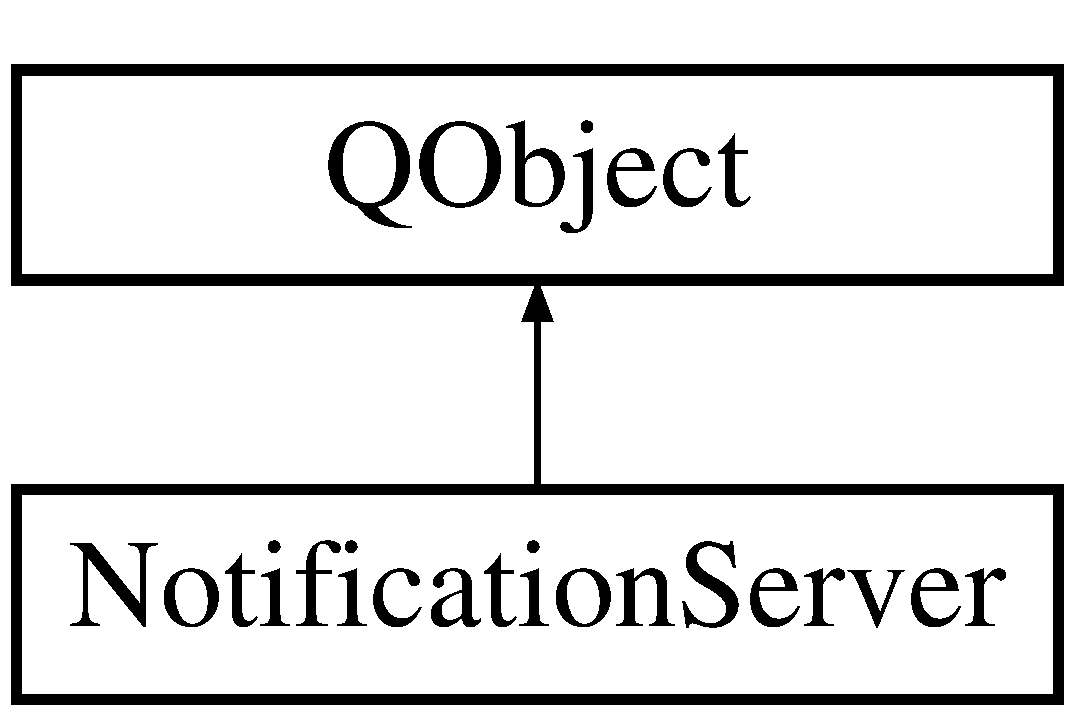
\includegraphics[height=2.000000cm]{class_notification_server}
\end{center}
\end{figure}
\subsection*{Public Slots}
\begin{DoxyCompactItemize}
\item 
\mbox{\Hypertarget{class_notification_server_a05d958280d812baf1e8a58c1be2f6537}\label{class_notification_server_a05d958280d812baf1e8a58c1be2f6537}} 
void {\bfseries send\+Notification\+Message} (const Q\+String \&uri, const Q\+Json\+Object \&obj)
\end{DoxyCompactItemize}
\subsection*{Signals}
\begin{DoxyCompactItemize}
\item 
\mbox{\Hypertarget{class_notification_server_afd67abdb7fcb7a06878e85a3f9f203b2}\label{class_notification_server_afd67abdb7fcb7a06878e85a3f9f203b2}} 
void {\bfseries broadcast\+Text\+Message} (const Q\+String \&message)
\end{DoxyCompactItemize}
\subsection*{Public Member Functions}
\begin{DoxyCompactItemize}
\item 
\mbox{\Hypertarget{class_notification_server_a02f5762b8e41d1677163d13805d47906}\label{class_notification_server_a02f5762b8e41d1677163d13805d47906}} 
{\bfseries Notification\+Server} (Q\+Object $\ast$parent=0)
\item 
\mbox{\Hypertarget{class_notification_server_a5e3a7df82c765939764c64a31339658e}\label{class_notification_server_a5e3a7df82c765939764c64a31339658e}} 
void {\bfseries start\+Server} (quint16 port)
\end{DoxyCompactItemize}
\subsection*{Static Public Member Functions}
\begin{DoxyCompactItemize}
\item 
\mbox{\Hypertarget{class_notification_server_a44b03b731cade32841e472283f264f51}\label{class_notification_server_a44b03b731cade32841e472283f264f51}} 
static \hyperlink{class_notification_server}{Notification\+Server} $\ast$ {\bfseries instance} (void)
\end{DoxyCompactItemize}
\subsection*{Protected Slots}
\begin{DoxyCompactItemize}
\item 
\mbox{\Hypertarget{class_notification_server_a7bf3b28c919b178ad8749beb9be4822e}\label{class_notification_server_a7bf3b28c919b178ad8749beb9be4822e}} 
void {\bfseries on\+New\+Connection} (void)
\item 
\mbox{\Hypertarget{class_notification_server_ab6cfeb3d264f611116162e30a15b16a5}\label{class_notification_server_ab6cfeb3d264f611116162e30a15b16a5}} 
void {\bfseries process\+Text\+Message} (const Q\+String message)
\item 
\mbox{\Hypertarget{class_notification_server_a377b34fac98a48cf025d80421ef85036}\label{class_notification_server_a377b34fac98a48cf025d80421ef85036}} 
void {\bfseries process\+Binary\+Message} (const Q\+Byte\+Array message)
\item 
\mbox{\Hypertarget{class_notification_server_a7088db19422ae675874a6e61cbfc52c0}\label{class_notification_server_a7088db19422ae675874a6e61cbfc52c0}} 
void {\bfseries socket\+Disconnected} (void)
\end{DoxyCompactItemize}


The documentation for this class was generated from the following files\+:\begin{DoxyCompactItemize}
\item 
L\+C\+S\+Server/Notification\+Server.\+h\item 
L\+C\+S\+Server/Notification\+Server.\+cpp\end{DoxyCompactItemize}

\hypertarget{class_p_i_g_p_i_o}{}\section{P\+I\+G\+P\+IO Class Reference}
\label{class_p_i_g_p_i_o}\index{P\+I\+G\+P\+IO@{P\+I\+G\+P\+IO}}
Inheritance diagram for P\+I\+G\+P\+IO\+:\begin{figure}[H]
\begin{center}
\leavevmode
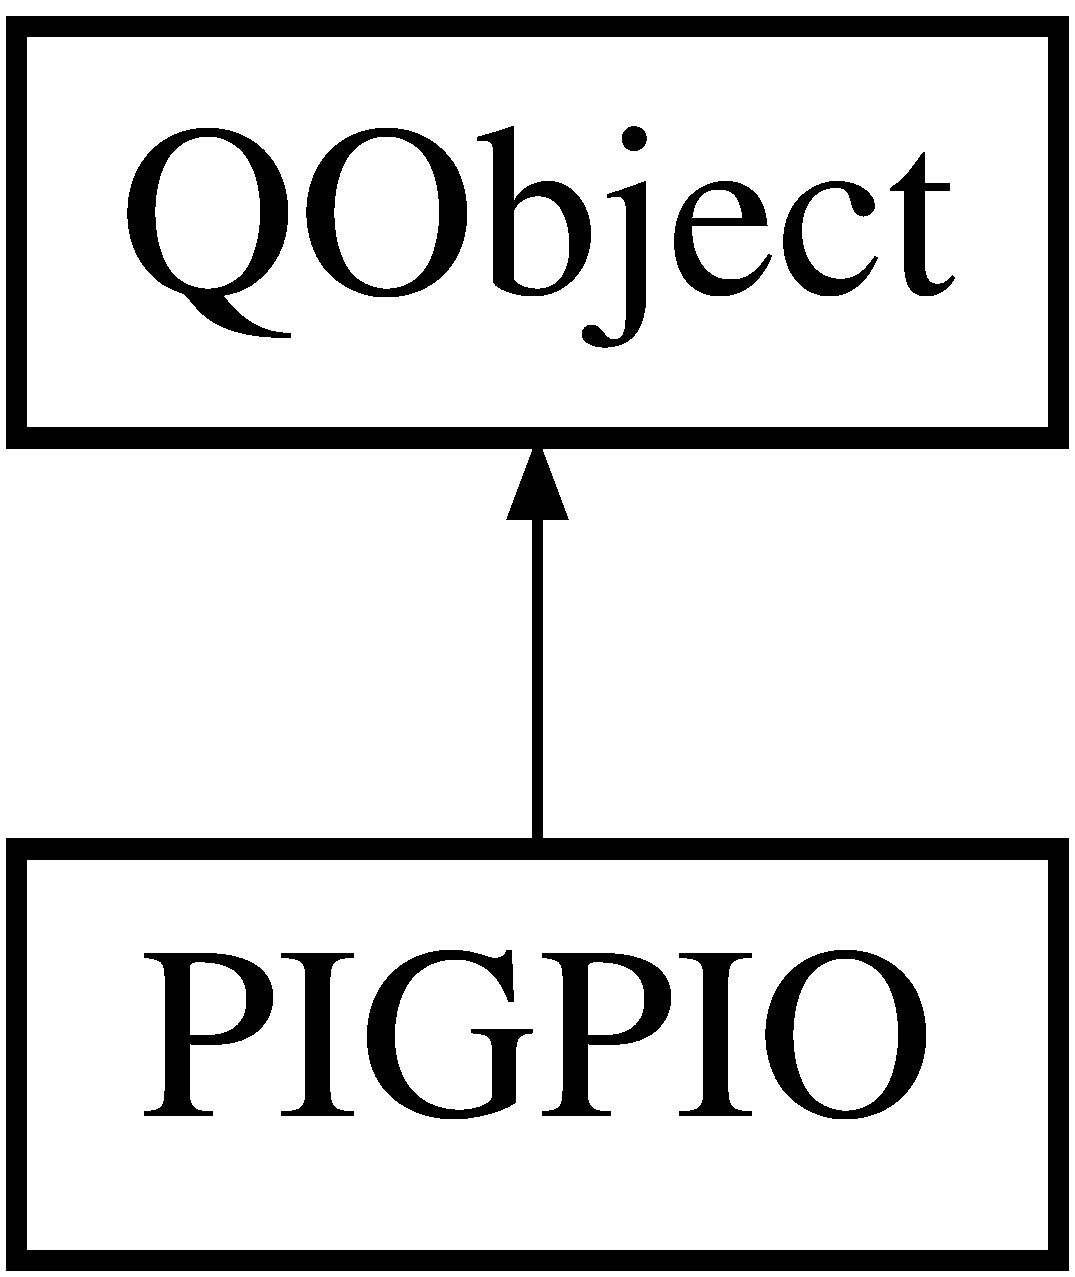
\includegraphics[height=2.000000cm]{class_p_i_g_p_i_o}
\end{center}
\end{figure}
\subsection*{Public Slots}
\begin{DoxyCompactItemize}
\item 
\mbox{\Hypertarget{class_p_i_g_p_i_o_aac1cb359875f9e188797f6246fc63641}\label{class_p_i_g_p_i_o_aac1cb359875f9e188797f6246fc63641}} 
void {\bfseries monitor\+Pin} (int pin)
\end{DoxyCompactItemize}
\subsection*{Signals}
\begin{DoxyCompactItemize}
\item 
\mbox{\Hypertarget{class_p_i_g_p_i_o_ad042c24e5cfaf8a505c1a08afe5cec53}\label{class_p_i_g_p_i_o_ad042c24e5cfaf8a505c1a08afe5cec53}} 
void {\bfseries pin\+Changed} (int pin, int value)
\end{DoxyCompactItemize}
\subsection*{Public Member Functions}
\begin{DoxyCompactItemize}
\item 
\mbox{\Hypertarget{class_p_i_g_p_i_o_ad16734c836686d7d1c565774d64292fe}\label{class_p_i_g_p_i_o_ad16734c836686d7d1c565774d64292fe}} 
{\bfseries P\+I\+G\+P\+IO} (Q\+Object $\ast$parent=0)
\item 
\mbox{\Hypertarget{class_p_i_g_p_i_o_a0a5a0e07fdf57c7a922ba9980fc0ea7b}\label{class_p_i_g_p_i_o_a0a5a0e07fdf57c7a922ba9980fc0ea7b}} 
bool {\bfseries pin\+Direction} (int pin, int dir)
\item 
\mbox{\Hypertarget{class_p_i_g_p_i_o_a30eb801cfb8fb73e290aacd29464ec2c}\label{class_p_i_g_p_i_o_a30eb801cfb8fb73e290aacd29464ec2c}} 
int {\bfseries read\+Pin} (int pin)
\item 
\mbox{\Hypertarget{class_p_i_g_p_i_o_a1f676b4254f7959c3df82b8d326bc450}\label{class_p_i_g_p_i_o_a1f676b4254f7959c3df82b8d326bc450}} 
int {\bfseries pin\+Write} (int pin, int value)
\end{DoxyCompactItemize}
\subsection*{Protected Slots}
\begin{DoxyCompactItemize}
\item 
\mbox{\Hypertarget{class_p_i_g_p_i_o_ad14366d5bc2af5abedf226b6557e12df}\label{class_p_i_g_p_i_o_ad14366d5bc2af5abedf226b6557e12df}} 
void {\bfseries timer\+Proc} (void)
\end{DoxyCompactItemize}


The documentation for this class was generated from the following files\+:\begin{DoxyCompactItemize}
\item 
L\+C\+S\+Server/P\+I\+G\+P\+I\+O.\+h\item 
L\+C\+S\+Server/P\+I\+G\+P\+I\+O.\+cpp\end{DoxyCompactItemize}

\hypertarget{class_qt_service}{}\section{Qt\+Service$<$ Application $>$ Class Template Reference}
\label{class_qt_service}\index{Qt\+Service$<$ Application $>$@{Qt\+Service$<$ Application $>$}}


The \hyperlink{class_qt_service}{Qt\+Service} is a convenient template class that allows you to create a service for a particular application type.  


Inheritance diagram for Qt\+Service$<$ Application $>$\+:\begin{figure}[H]
\begin{center}
\leavevmode
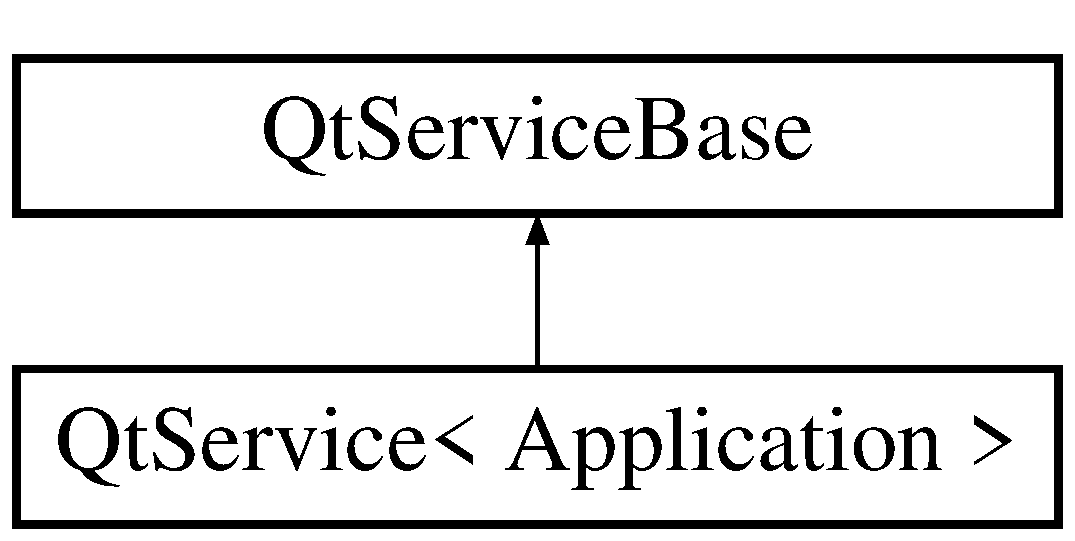
\includegraphics[height=2.000000cm]{class_qt_service}
\end{center}
\end{figure}
\subsection*{Public Member Functions}
\begin{DoxyCompactItemize}
\item 
\hyperlink{class_qt_service_aca39304919f89cbb95fca64f44a761ae}{Qt\+Service} (int argc, char $\ast$$\ast$argv, const Q\+String \&name)
\item 
\hyperlink{class_qt_service_a96af408261dfa13bd8034f67949d6c2d}{$\sim$\+Qt\+Service} ()
\end{DoxyCompactItemize}
\subsection*{Protected Member Functions}
\begin{DoxyCompactItemize}
\item 
Application $\ast$ \hyperlink{class_qt_service_a39743415a6ece5c7c6e6b5b01289c00b}{application} () const
\item 
virtual void \hyperlink{class_qt_service_a50aa2079345abfd0b1284be47e245b0b}{create\+Application} (int \&argc, char $\ast$$\ast$argv)
\item 
virtual int \hyperlink{class_qt_service_a84f5f60304117e1f11cc0ed16dc0b72e}{execute\+Application} ()
\end{DoxyCompactItemize}
\subsection*{Additional Inherited Members}


\subsection{Detailed Description}
\subsubsection*{template$<$typename Application$>$\newline
class Qt\+Service$<$ Application $>$}

The \hyperlink{class_qt_service}{Qt\+Service} is a convenient template class that allows you to create a service for a particular application type. 

A Windows service or Unix daemon (a \char`\"{}service\char`\"{}), is a program that runs \char`\"{}in the background\char`\"{} independently of whether a user is logged in or not. A service is often set up to start when the machine boots up, and will typically run continuously as long as the machine is on.

Services are usually non-\/interactive console applications. User interaction, if required, is usually implemented in a separate, normal G\+UI application that communicates with the service through an I\+PC channel. For simple communication, \hyperlink{class_qt_service_controller_a1428c7d51403416bc7663ae37c446cfc}{Qt\+Service\+Controller\+::send\+Command()} and \hyperlink{class_qt_service_base_a47485f00f6eba0758d2ffc75092295cf}{Qt\+Service\+::process\+Command()} may be used, possibly in combination with a shared settings file. For more complex, interactive communication, a custom I\+PC channel should be used, e.\+g. based on Qt\textquotesingle{}s networking classes. (In certain circumstances, a service may provide a G\+UI itself, ref. the \char`\"{}interactive\char`\"{} example documentation).

\{Note\+:\} On Unix systems, this class relies on facilities provided by the Qt\+Network module, provided as part of the \{Qt Open Source Edition\} and certain \{Qt Commercial Editions\}.

The \hyperlink{class_qt_service}{Qt\+Service} class functionality is inherited from \hyperlink{class_qt_service_base}{Qt\+Service\+Base}, but in addition the \hyperlink{class_qt_service}{Qt\+Service} class binds an instance of \hyperlink{class_qt_service_base}{Qt\+Service\+Base} with an application type.

Typically, you will create a service by subclassing the \hyperlink{class_qt_service}{Qt\+Service} template class. For example\+:


\begin{DoxyCode}
\textcolor{keyword}{class }MyService : \textcolor{keyword}{public} \hyperlink{class_qt_service}{QtService}<QApplication>
\{
\textcolor{keyword}{public}:
    MyService(\textcolor{keywordtype}{int} argc, \textcolor{keywordtype}{char} **argv);
    ~MyService();

\textcolor{keyword}{protected}:
    \textcolor{keywordtype}{void} \hyperlink{class_qt_service_base_adbc0cd621b41bd3a6a1f62fda432e9e4}{start}();
    \textcolor{keywordtype}{void} \hyperlink{class_qt_service_base_a8d52c1b8fd06b50bdc0a0c6f9936a68e}{stop}();
    \textcolor{keywordtype}{void} \hyperlink{class_qt_service_base_a43215a7c5c047d30bcf4f697e6691f89}{pause}();
    \textcolor{keywordtype}{void} \hyperlink{class_qt_service_base_aaa2e05ef1c36283b6b35348c3972b489}{resume}();
    \textcolor{keywordtype}{void} \hyperlink{class_qt_service_base_a47485f00f6eba0758d2ffc75092295cf}{processCommand}(\textcolor{keywordtype}{int} code);
\};
\end{DoxyCode}


The application type can be Q\+Core\+Application for services without G\+UI, Q\+Application for services with G\+UI or you can use your own custom application type.

You must reimplement the \hyperlink{class_qt_service_base_adbc0cd621b41bd3a6a1f62fda432e9e4}{Qt\+Service\+Base\+::start()} function to perform the service\textquotesingle{}s work. Usually you create some main object on the heap which is the heart of your service.

In addition, you might want to reimplement the \hyperlink{class_qt_service_base_a43215a7c5c047d30bcf4f697e6691f89}{Qt\+Service\+Base\+::pause()}, \hyperlink{class_qt_service_base_a47485f00f6eba0758d2ffc75092295cf}{Qt\+Service\+Base\+::process\+Command()}, \hyperlink{class_qt_service_base_aaa2e05ef1c36283b6b35348c3972b489}{Qt\+Service\+Base\+::resume()} and \hyperlink{class_qt_service_base_a8d52c1b8fd06b50bdc0a0c6f9936a68e}{Qt\+Service\+Base\+::stop()} to intervene the service\textquotesingle{}s process on controller requests. You can control any given service using an instance of the \hyperlink{class_qt_service_controller}{Qt\+Service\+Controller} class which also allows you to control services from separate applications. The mentioned functions are all virtual and won\textquotesingle{}t do anything unless they are reimplemented.

Your custom service is typically instantiated in the application\textquotesingle{}s main function. Then the main function will call your service\textquotesingle{}s \hyperlink{class_qt_service_base_afae2e589de71c1ae3ae8db3dc9ab9c64}{exec()} function, and return the result of that call. For example\+:


\begin{DoxyCode}
\textcolor{keywordtype}{int} main(\textcolor{keywordtype}{int} argc, \textcolor{keywordtype}{char} **argv)
\{
    MyService service(argc, argv);
    \textcolor{keywordflow}{return} service.exec();
\}
\end{DoxyCode}


When the \hyperlink{class_qt_service_base_afae2e589de71c1ae3ae8db3dc9ab9c64}{exec()} function is called, it will parse the  \{service\+Specific\+Arguments\} \{service specific arguments\} passed in {\ttfamily argv}, perform the required actions, and exit.

If none of the arguments is recognized as service specific, \hyperlink{class_qt_service_base_afae2e589de71c1ae3ae8db3dc9ab9c64}{exec()} will first call the \hyperlink{class_qt_service_a50aa2079345abfd0b1284be47e245b0b}{create\+Application()} function, then \hyperlink{class_qt_service_a84f5f60304117e1f11cc0ed16dc0b72e}{execute\+Application()} and finally the \hyperlink{class_qt_service_base_adbc0cd621b41bd3a6a1f62fda432e9e4}{start()} function. In the end, \hyperlink{class_qt_service_base_afae2e589de71c1ae3ae8db3dc9ab9c64}{exec()} returns while the service continues in its own process waiting for commands from the service controller.

\begin{DoxySeeAlso}{See also}
\hyperlink{class_qt_service_base}{Qt\+Service\+Base}, \hyperlink{class_qt_service_controller}{Qt\+Service\+Controller} 
\end{DoxySeeAlso}


\subsection{Constructor \& Destructor Documentation}
\mbox{\Hypertarget{class_qt_service_aca39304919f89cbb95fca64f44a761ae}\label{class_qt_service_aca39304919f89cbb95fca64f44a761ae}} 
\index{Qt\+Service@{Qt\+Service}!Qt\+Service@{Qt\+Service}}
\index{Qt\+Service@{Qt\+Service}!Qt\+Service@{Qt\+Service}}
\subsubsection{\texorpdfstring{Qt\+Service()}{QtService()}}
{\footnotesize\ttfamily template$<$typename Application$>$ \\
\hyperlink{class_qt_service}{Qt\+Service}$<$ Application $>$\+::\hyperlink{class_qt_service}{Qt\+Service} (\begin{DoxyParamCaption}\item[{int}]{argc,  }\item[{char $\ast$$\ast$}]{argv,  }\item[{const Q\+String \&}]{name }\end{DoxyParamCaption})\hspace{0.3cm}{\ttfamily [inline]}}

Constructs a \hyperlink{class_qt_service}{Qt\+Service} object called {\itshape name}. The {\itshape argc} and {\itshape argv} parameters are parsed after the \hyperlink{class_qt_service_base_afae2e589de71c1ae3ae8db3dc9ab9c64}{exec()} function has been called. Then they are passed to the application\textquotesingle{}s constructor.

There can only be one \hyperlink{class_qt_service}{Qt\+Service} object in a process.

\begin{DoxySeeAlso}{See also}
\hyperlink{class_qt_service_base_a75e3f82739df6dc0b9aa899b3f9552eb}{Qt\+Service\+Base()} 
\end{DoxySeeAlso}
\mbox{\Hypertarget{class_qt_service_a96af408261dfa13bd8034f67949d6c2d}\label{class_qt_service_a96af408261dfa13bd8034f67949d6c2d}} 
\index{Qt\+Service@{Qt\+Service}!````~Qt\+Service@{$\sim$\+Qt\+Service}}
\index{````~Qt\+Service@{$\sim$\+Qt\+Service}!Qt\+Service@{Qt\+Service}}
\subsubsection{\texorpdfstring{$\sim$\+Qt\+Service()}{~QtService()}}
{\footnotesize\ttfamily template$<$typename Application$>$ \\
\hyperlink{class_qt_service}{Qt\+Service}$<$ Application $>$\+::$\sim$\hyperlink{class_qt_service}{Qt\+Service} (\begin{DoxyParamCaption}{ }\end{DoxyParamCaption})\hspace{0.3cm}{\ttfamily [inline]}}

Destroys the service object. 

\subsection{Member Function Documentation}
\mbox{\Hypertarget{class_qt_service_a39743415a6ece5c7c6e6b5b01289c00b}\label{class_qt_service_a39743415a6ece5c7c6e6b5b01289c00b}} 
\index{Qt\+Service@{Qt\+Service}!application@{application}}
\index{application@{application}!Qt\+Service@{Qt\+Service}}
\subsubsection{\texorpdfstring{application()}{application()}}
{\footnotesize\ttfamily template$<$typename Application$>$ \\
Application $\ast$ \hyperlink{class_qt_service}{Qt\+Service}$<$ Application $>$\+::application (\begin{DoxyParamCaption}{ }\end{DoxyParamCaption}) const\hspace{0.3cm}{\ttfamily [inline]}, {\ttfamily [protected]}}

Returns a pointer to the application object. \mbox{\Hypertarget{class_qt_service_a50aa2079345abfd0b1284be47e245b0b}\label{class_qt_service_a50aa2079345abfd0b1284be47e245b0b}} 
\index{Qt\+Service@{Qt\+Service}!create\+Application@{create\+Application}}
\index{create\+Application@{create\+Application}!Qt\+Service@{Qt\+Service}}
\subsubsection{\texorpdfstring{create\+Application()}{createApplication()}}
{\footnotesize\ttfamily template$<$typename Application$>$ \\
void \hyperlink{class_qt_service}{Qt\+Service}$<$ Application $>$\+::create\+Application (\begin{DoxyParamCaption}\item[{int \&}]{argc,  }\item[{char $\ast$$\ast$}]{argv }\end{DoxyParamCaption})\hspace{0.3cm}{\ttfamily [inline]}, {\ttfamily [protected]}, {\ttfamily [virtual]}}

Creates application object of type Application passing {\itshape argc} and {\itshape argv} to its constructor.

Implements \hyperlink{class_qt_service_base_ac5ae73935f489282b35c70b27b341390}{Qt\+Service\+Base}.

\mbox{\Hypertarget{class_qt_service_a84f5f60304117e1f11cc0ed16dc0b72e}\label{class_qt_service_a84f5f60304117e1f11cc0ed16dc0b72e}} 
\index{Qt\+Service@{Qt\+Service}!execute\+Application@{execute\+Application}}
\index{execute\+Application@{execute\+Application}!Qt\+Service@{Qt\+Service}}
\subsubsection{\texorpdfstring{execute\+Application()}{executeApplication()}}
{\footnotesize\ttfamily template$<$typename Application$>$ \\
int \hyperlink{class_qt_service}{Qt\+Service}$<$ Application $>$\+::execute\+Application (\begin{DoxyParamCaption}{ }\end{DoxyParamCaption})\hspace{0.3cm}{\ttfamily [inline]}, {\ttfamily [protected]}, {\ttfamily [virtual]}}



Implements \hyperlink{class_qt_service_base_ab70633cd29a22758dfa0502b77e564f6}{Qt\+Service\+Base}.



The documentation for this class was generated from the following files\+:\begin{DoxyCompactItemize}
\item 
L\+C\+S\+Server/\+Qt\+Solutions\+Service/src/qtservice.\+h\item 
L\+C\+S\+Server/\+Qt\+Solutions\+Service/src/qtservice.\+cpp\end{DoxyCompactItemize}

\hypertarget{class_qt_service_base}{}\section{Qt\+Service\+Base Class Reference}
\label{class_qt_service_base}\index{Qt\+Service\+Base@{Qt\+Service\+Base}}


The \hyperlink{class_qt_service_base}{Qt\+Service\+Base} class provides an A\+PI for implementing Windows services and Unix daemons.  


Inheritance diagram for Qt\+Service\+Base\+:\begin{figure}[H]
\begin{center}
\leavevmode
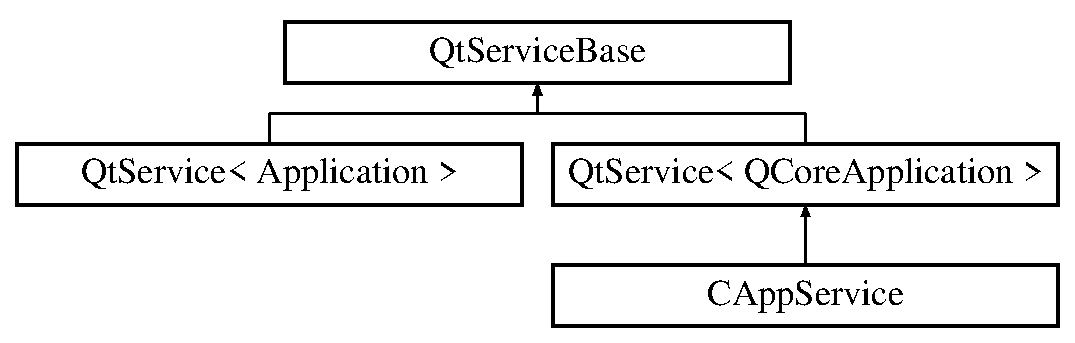
\includegraphics[height=3.000000cm]{class_qt_service_base}
\end{center}
\end{figure}
\subsection*{Public Types}
\begin{DoxyCompactItemize}
\item 
enum \hyperlink{class_qt_service_base_acffd9389fe7178bf1f35d8bf3dae1095}{Message\+Type} \{ {\bfseries Success} = 0, 
{\bfseries Error}, 
{\bfseries Warning}, 
{\bfseries Information}
 \}
\item 
enum \hyperlink{class_qt_service_base_af6e74a87329ef64760783364538e5d51}{Service\+Flag} \{ {\bfseries Default} = 0x00, 
{\bfseries Can\+Be\+Suspended} = 0x01, 
{\bfseries Cannot\+Be\+Stopped} = 0x02, 
{\bfseries Needs\+Stop\+On\+Shutdown} = 0x04
 \}
\end{DoxyCompactItemize}
\subsection*{Public Member Functions}
\begin{DoxyCompactItemize}
\item 
\hyperlink{class_qt_service_base_a75e3f82739df6dc0b9aa899b3f9552eb}{Qt\+Service\+Base} (int argc, char $\ast$$\ast$argv, const Q\+String \&name)
\item 
virtual \hyperlink{class_qt_service_base_a82c0872e5ed2448eff9eb6521f75bfd2}{$\sim$\+Qt\+Service\+Base} ()
\item 
Q\+String \hyperlink{class_qt_service_base_a643f253b3931e6a6c4e8caa190756214}{service\+Name} () const
\item 
Q\+String \hyperlink{class_qt_service_base_a6cf3ef7bc5d85acb31e99a85fde47397}{service\+Description} () const
\item 
void \hyperlink{class_qt_service_base_a09d7547436c65a900f18c58b2a650286}{set\+Service\+Description} (const Q\+String \&description)
\item 
\hyperlink{class_qt_service_controller_a946ac2b079d9760503da923c2eaf0aac}{Qt\+Service\+Controller\+::\+Startup\+Type} \hyperlink{class_qt_service_base_aa1b3bf9b7fc09777b422f49f7bcfbcbe}{startup\+Type} () const
\item 
void \hyperlink{class_qt_service_base_a6beddd54c973c3a7d81075b2f3f80df2}{set\+Startup\+Type} (\hyperlink{class_qt_service_controller_a946ac2b079d9760503da923c2eaf0aac}{Qt\+Service\+Controller\+::\+Startup\+Type} \hyperlink{class_qt_service_base_aa1b3bf9b7fc09777b422f49f7bcfbcbe}{startup\+Type})
\item 
Service\+Flags \hyperlink{class_qt_service_base_aab0b204981c481e098fe72061e3f367a}{service\+Flags} () const
\item 
void \hyperlink{class_qt_service_base_a3f8a07d0cf536720e7fcf1ec562635d1}{set\+Service\+Flags} (Service\+Flags flags)
\item 
int \hyperlink{class_qt_service_base_afae2e589de71c1ae3ae8db3dc9ab9c64}{exec} ()
\item 
void \hyperlink{class_qt_service_base_ac071ce0b30547e17c3b3ca9dcb0108c9}{log\+Message} (const Q\+String \&message, \hyperlink{class_qt_service_base_acffd9389fe7178bf1f35d8bf3dae1095}{Message\+Type} type=Success, int id=0, uint category=0, const Q\+Byte\+Array \&data=Q\+Byte\+Array())
\end{DoxyCompactItemize}
\subsection*{Static Public Member Functions}
\begin{DoxyCompactItemize}
\item 
static \hyperlink{class_qt_service_base}{Qt\+Service\+Base} $\ast$ \hyperlink{class_qt_service_base_a8f030376e32cc47736bfc1a1e1ecf855}{instance} ()
\end{DoxyCompactItemize}
\subsection*{Protected Member Functions}
\begin{DoxyCompactItemize}
\item 
virtual void \hyperlink{class_qt_service_base_adbc0cd621b41bd3a6a1f62fda432e9e4}{start} ()=0
\item 
virtual void \hyperlink{class_qt_service_base_a8d52c1b8fd06b50bdc0a0c6f9936a68e}{stop} ()
\item 
virtual void \hyperlink{class_qt_service_base_a43215a7c5c047d30bcf4f697e6691f89}{pause} ()
\item 
virtual void \hyperlink{class_qt_service_base_aaa2e05ef1c36283b6b35348c3972b489}{resume} ()
\item 
virtual void \hyperlink{class_qt_service_base_a47485f00f6eba0758d2ffc75092295cf}{process\+Command} (int code)
\item 
virtual void \hyperlink{class_qt_service_base_ac5ae73935f489282b35c70b27b341390}{create\+Application} (int \&argc, char $\ast$$\ast$argv)=0
\item 
virtual int \hyperlink{class_qt_service_base_ab70633cd29a22758dfa0502b77e564f6}{execute\+Application} ()=0
\end{DoxyCompactItemize}
\subsection*{Friends}
\begin{DoxyCompactItemize}
\item 
\mbox{\Hypertarget{class_qt_service_base_a3101d1ae35029ba305c82b8f49512d6f}\label{class_qt_service_base_a3101d1ae35029ba305c82b8f49512d6f}} 
class {\bfseries Qt\+Service\+Sys\+Private}
\end{DoxyCompactItemize}


\subsection{Detailed Description}
The \hyperlink{class_qt_service_base}{Qt\+Service\+Base} class provides an A\+PI for implementing Windows services and Unix daemons. 

A Windows service or Unix daemon (a \char`\"{}service\char`\"{}), is a program that runs \char`\"{}in the background\char`\"{} independently of whether a user is logged in or not. A service is often set up to start when the machine boots up, and will typically run continuously as long as the machine is on.

Services are usually non-\/interactive console applications. User interaction, if required, is usually implemented in a separate, normal G\+UI application that communicates with the service through an I\+PC channel. For simple communication, \hyperlink{class_qt_service_controller_a1428c7d51403416bc7663ae37c446cfc}{Qt\+Service\+Controller\+::send\+Command()} and \hyperlink{class_qt_service_base_a47485f00f6eba0758d2ffc75092295cf}{Qt\+Service\+::process\+Command()} may be used, possibly in combination with a shared settings file. For more complex, interactive communication, a custom I\+PC channel should be used, e.\+g. based on Qt\textquotesingle{}s networking classes. (In certain circumstances, a service may provide a G\+UI itself, ref. the \char`\"{}interactive\char`\"{} example documentation).

Typically, you will create a service by subclassing the \hyperlink{class_qt_service}{Qt\+Service} template class which inherits \hyperlink{class_qt_service_base}{Qt\+Service\+Base} and allows you to create a service for a particular application type.

The Windows implementation uses the NT Service Control Manager, and the application can be controlled through the system administration tools. Services are usually launched using the system account, which requires that all D\+L\+Ls that the service executable depends on (i.\+e. Qt), are located in the same directory as the service, or in a system path.

On Unix a service is implemented as a daemon.

You can retrieve the service\textquotesingle{}s description, state, and startup type using the \hyperlink{class_qt_service_base_a6cf3ef7bc5d85acb31e99a85fde47397}{service\+Description()}, \hyperlink{class_qt_service_base_aab0b204981c481e098fe72061e3f367a}{service\+Flags()} and \hyperlink{class_qt_service_base_aa1b3bf9b7fc09777b422f49f7bcfbcbe}{startup\+Type()} functions respectively. The service\textquotesingle{}s state is decribed by the Service\+Flag enum. The mentioned properites can also be set using the corresponding set functions. In addition you can retrieve the service\textquotesingle{}s name using the \hyperlink{class_qt_service_base_a643f253b3931e6a6c4e8caa190756214}{service\+Name()} function.

Several of \hyperlink{class_qt_service_base}{Qt\+Service\+Base}\textquotesingle{}s protected functions are called on requests from the \hyperlink{class_qt_service_controller}{Qt\+Service\+Controller} class\+:

\hyperlink{class_qt_service_base_adbc0cd621b41bd3a6a1f62fda432e9e4}{start()}  \hyperlink{class_qt_service_base_a43215a7c5c047d30bcf4f697e6691f89}{pause()}  \hyperlink{class_qt_service_base_a47485f00f6eba0758d2ffc75092295cf}{process\+Command()}  \hyperlink{class_qt_service_base_aaa2e05ef1c36283b6b35348c3972b489}{resume()}  \hyperlink{class_qt_service_base_a8d52c1b8fd06b50bdc0a0c6f9936a68e}{stop()} 

You can control any given service using an instance of the \hyperlink{class_qt_service_controller}{Qt\+Service\+Controller} class which also allows you to control services from separate applications. The mentioned functions are all virtual and won\textquotesingle{}t do anything unless they are reimplemented. You can reimplement these functions to pause and resume the service\textquotesingle{}s execution, as well as process user commands and perform additional clean-\/ups before shutting down.

\hyperlink{class_qt_service_base}{Qt\+Service\+Base} also provides the static \hyperlink{class_qt_service_base_a8f030376e32cc47736bfc1a1e1ecf855}{instance()} function which returns a pointer to an application\textquotesingle{}s \hyperlink{class_qt_service_base}{Qt\+Service\+Base} instance. In addition, a service can report events to the system\textquotesingle{}s event log using the \hyperlink{class_qt_service_base_ac071ce0b30547e17c3b3ca9dcb0108c9}{log\+Message()} function. The Message\+Type enum describes the different types of messages a service reports.

The implementation of a service application\textquotesingle{}s main function typically creates an service object derived by subclassing the \hyperlink{class_qt_service}{Qt\+Service} template class. Then the main function will call this service\textquotesingle{}s \hyperlink{class_qt_service_base_afae2e589de71c1ae3ae8db3dc9ab9c64}{exec()} function, and return the result of that call. For example\+:


\begin{DoxyCode}
\textcolor{keywordtype}{int} main(\textcolor{keywordtype}{int} argc, \textcolor{keywordtype}{char} **argv)
\{
    MyService service(argc, argv);
    \textcolor{keywordflow}{return} service.exec();
\}
\end{DoxyCode}


When the \hyperlink{class_qt_service_base_afae2e589de71c1ae3ae8db3dc9ab9c64}{exec()} function is called, it will parse the service specific arguments passed in {\ttfamily argv}, perform the required actions, and return.

service\+Specific\+Arguments

The following arguments are recognized as service specific\+:

Short  Long  Explanation   -\/i  -\/install  Install the service.   -\/u  -\/uninstall  Uninstall the service.   -\/e  -\/exec  Execute the service as a standalone application (useful for debug purposes). This is a blocking call, the service will be executed like a normal application. In this mode you will not be able to communicate with the service from the contoller.   -\/t  -\/terminate  Stop the service.   -\/p  -\/pause  Pause the service.   -\/r  -\/resume  Resume a paused service.   -\/c {\itshape }\{cmd\}  -\/command {\itshape }\{cmd\}  Send the user defined command code {\itshape }\{cmd\} to the service application.   -\/v  -\/version  Display version and status information. 

If {\itshape none} of the arguments is recognized as service specific, \hyperlink{class_qt_service_base_afae2e589de71c1ae3ae8db3dc9ab9c64}{exec()} will first call the \hyperlink{class_qt_service_base_ac5ae73935f489282b35c70b27b341390}{create\+Application()} function, then \hyperlink{class_qt_service_base_ab70633cd29a22758dfa0502b77e564f6}{execute\+Application()} and finally the \hyperlink{class_qt_service_base_adbc0cd621b41bd3a6a1f62fda432e9e4}{start()} function. In the end, \hyperlink{class_qt_service_base_afae2e589de71c1ae3ae8db3dc9ab9c64}{exec()} returns while the service continues in its own process waiting for commands from the service controller.

\begin{DoxySeeAlso}{See also}
\hyperlink{class_qt_service}{Qt\+Service}, \hyperlink{class_qt_service_controller}{Qt\+Service\+Controller} 
\end{DoxySeeAlso}


\subsection{Member Enumeration Documentation}
\mbox{\Hypertarget{class_qt_service_base_acffd9389fe7178bf1f35d8bf3dae1095}\label{class_qt_service_base_acffd9389fe7178bf1f35d8bf3dae1095}} 
\index{Qt\+Service\+Base@{Qt\+Service\+Base}!Message\+Type@{Message\+Type}}
\index{Message\+Type@{Message\+Type}!Qt\+Service\+Base@{Qt\+Service\+Base}}
\subsubsection{\texorpdfstring{Message\+Type}{MessageType}}
{\footnotesize\ttfamily enum \hyperlink{class_qt_service_base_acffd9389fe7178bf1f35d8bf3dae1095}{Qt\+Service\+Base\+::\+Message\+Type}}

This enum describes the different types of messages a service reports to the system log.

Success An operation has succeeded, e.\+g. the service is started.  Error An operation failed, e.\+g. the service failed to start.  Warning An operation caused a warning that might require user interaction.  Information Any type of usually non-\/critical information. \mbox{\Hypertarget{class_qt_service_base_af6e74a87329ef64760783364538e5d51}\label{class_qt_service_base_af6e74a87329ef64760783364538e5d51}} 
\index{Qt\+Service\+Base@{Qt\+Service\+Base}!Service\+Flag@{Service\+Flag}}
\index{Service\+Flag@{Service\+Flag}!Qt\+Service\+Base@{Qt\+Service\+Base}}
\subsubsection{\texorpdfstring{Service\+Flag}{ServiceFlag}}
{\footnotesize\ttfamily enum \hyperlink{class_qt_service_base_af6e74a87329ef64760783364538e5d51}{Qt\+Service\+Base\+::\+Service\+Flag}}

This enum describes the different capabilities of a service.

Default The service can be stopped, but not suspended.  Can\+Be\+Suspended The service can be suspended.  Cannot\+Be\+Stopped The service cannot be stopped.  Needs\+Stop\+On\+Shutdown (Windows only) The service will be stopped before the system shuts down. Note that Microsoft recommends this only for services that must absolutely clean up during shutdown, because there is a limited time available for shutdown of services. 

\subsection{Constructor \& Destructor Documentation}
\mbox{\Hypertarget{class_qt_service_base_a75e3f82739df6dc0b9aa899b3f9552eb}\label{class_qt_service_base_a75e3f82739df6dc0b9aa899b3f9552eb}} 
\index{Qt\+Service\+Base@{Qt\+Service\+Base}!Qt\+Service\+Base@{Qt\+Service\+Base}}
\index{Qt\+Service\+Base@{Qt\+Service\+Base}!Qt\+Service\+Base@{Qt\+Service\+Base}}
\subsubsection{\texorpdfstring{Qt\+Service\+Base()}{QtServiceBase()}}
{\footnotesize\ttfamily Qt\+Service\+Base\+::\+Qt\+Service\+Base (\begin{DoxyParamCaption}\item[{int}]{argc,  }\item[{char $\ast$$\ast$}]{argv,  }\item[{const Q\+String \&}]{name }\end{DoxyParamCaption})}

Creates a service instance called {\itshape name}. The {\itshape argc} and {\itshape argv} parameters are parsed after the \hyperlink{class_qt_service_base_afae2e589de71c1ae3ae8db3dc9ab9c64}{exec()} function has been called. Then they are passed to the application\textquotesingle{}s constructor. The application type is determined by the \hyperlink{class_qt_service}{Qt\+Service} subclass.

The service is neither installed nor started. The name must not contain any backslashes or be longer than 255 characters. In addition, the name must be unique in the system\textquotesingle{}s service database.

\begin{DoxySeeAlso}{See also}
\hyperlink{class_qt_service_base_afae2e589de71c1ae3ae8db3dc9ab9c64}{exec()}, \hyperlink{class_qt_service_base_adbc0cd621b41bd3a6a1f62fda432e9e4}{start()}, \hyperlink{class_qt_service_controller_a7e2b85e911ff152557dd25959e76094b}{Qt\+Service\+Controller\+::install()} 
\end{DoxySeeAlso}
\mbox{\Hypertarget{class_qt_service_base_a82c0872e5ed2448eff9eb6521f75bfd2}\label{class_qt_service_base_a82c0872e5ed2448eff9eb6521f75bfd2}} 
\index{Qt\+Service\+Base@{Qt\+Service\+Base}!````~Qt\+Service\+Base@{$\sim$\+Qt\+Service\+Base}}
\index{````~Qt\+Service\+Base@{$\sim$\+Qt\+Service\+Base}!Qt\+Service\+Base@{Qt\+Service\+Base}}
\subsubsection{\texorpdfstring{$\sim$\+Qt\+Service\+Base()}{~QtServiceBase()}}
{\footnotesize\ttfamily Qt\+Service\+Base\+::$\sim$\+Qt\+Service\+Base (\begin{DoxyParamCaption}{ }\end{DoxyParamCaption})\hspace{0.3cm}{\ttfamily [virtual]}}

Destroys the service object. This neither stops nor uninstalls the service.

To stop a service the \hyperlink{class_qt_service_base_a8d52c1b8fd06b50bdc0a0c6f9936a68e}{stop()} function must be called explicitly. To uninstall a service, you can use the \hyperlink{class_qt_service_controller_a25cd2f1f6868ece5de77976eb55cb74c}{Qt\+Service\+Controller\+::uninstall()} function.

\begin{DoxySeeAlso}{See also}
\hyperlink{class_qt_service_base_a8d52c1b8fd06b50bdc0a0c6f9936a68e}{stop()}, \hyperlink{class_qt_service_controller_a25cd2f1f6868ece5de77976eb55cb74c}{Qt\+Service\+Controller\+::uninstall()} 
\end{DoxySeeAlso}


\subsection{Member Function Documentation}
\mbox{\Hypertarget{class_qt_service_base_ac5ae73935f489282b35c70b27b341390}\label{class_qt_service_base_ac5ae73935f489282b35c70b27b341390}} 
\index{Qt\+Service\+Base@{Qt\+Service\+Base}!create\+Application@{create\+Application}}
\index{create\+Application@{create\+Application}!Qt\+Service\+Base@{Qt\+Service\+Base}}
\subsubsection{\texorpdfstring{create\+Application()}{createApplication()}}
{\footnotesize\ttfamily void Qt\+Service\+Base\+::create\+Application (\begin{DoxyParamCaption}\item[{int \&}]{argc,  }\item[{char $\ast$$\ast$}]{argv }\end{DoxyParamCaption})\hspace{0.3cm}{\ttfamily [protected]}, {\ttfamily [pure virtual]}}

Creates the application object using the {\itshape argc} and {\itshape argv} parameters.

This function is only called when no  \{service\+Specific\+Arguments\}\{service specific arguments\} were passed to the service constructor, and is called by \hyperlink{class_qt_service_base_afae2e589de71c1ae3ae8db3dc9ab9c64}{exec()} before it calls the \hyperlink{class_qt_service_base_ab70633cd29a22758dfa0502b77e564f6}{execute\+Application()} and \hyperlink{class_qt_service_base_adbc0cd621b41bd3a6a1f62fda432e9e4}{start()} functions.

The \hyperlink{class_qt_service_base_ac5ae73935f489282b35c70b27b341390}{create\+Application()} function is implemented in \hyperlink{class_qt_service}{Qt\+Service}, but you might want to reimplement it, for example, if the chosen application type\textquotesingle{}s constructor needs additional arguments.

\begin{DoxySeeAlso}{See also}
\hyperlink{class_qt_service_base_afae2e589de71c1ae3ae8db3dc9ab9c64}{exec()}, \hyperlink{class_qt_service}{Qt\+Service} 
\end{DoxySeeAlso}


Implemented in \hyperlink{class_qt_service_a50aa2079345abfd0b1284be47e245b0b}{Qt\+Service$<$ Application $>$}, and \hyperlink{class_qt_service_a50aa2079345abfd0b1284be47e245b0b}{Qt\+Service$<$ Q\+Core\+Application $>$}.

\mbox{\Hypertarget{class_qt_service_base_afae2e589de71c1ae3ae8db3dc9ab9c64}\label{class_qt_service_base_afae2e589de71c1ae3ae8db3dc9ab9c64}} 
\index{Qt\+Service\+Base@{Qt\+Service\+Base}!exec@{exec}}
\index{exec@{exec}!Qt\+Service\+Base@{Qt\+Service\+Base}}
\subsubsection{\texorpdfstring{exec()}{exec()}}
{\footnotesize\ttfamily int Qt\+Service\+Base\+::exec (\begin{DoxyParamCaption}{ }\end{DoxyParamCaption})}

Executes the service.

When the \hyperlink{class_qt_service_base_afae2e589de71c1ae3ae8db3dc9ab9c64}{exec()} function is called, it will parse the  \{service\+Specific\+Arguments\} \{service specific arguments\} passed in {\ttfamily argv}, perform the required actions, and exit.

If none of the arguments is recognized as service specific, \hyperlink{class_qt_service_base_afae2e589de71c1ae3ae8db3dc9ab9c64}{exec()} will first call the \hyperlink{class_qt_service_base_ac5ae73935f489282b35c70b27b341390}{create\+Application()} function, then \hyperlink{class_qt_service_base_ab70633cd29a22758dfa0502b77e564f6}{execute\+Application()} and finally the \hyperlink{class_qt_service_base_adbc0cd621b41bd3a6a1f62fda432e9e4}{start()} function. In the end, \hyperlink{class_qt_service_base_afae2e589de71c1ae3ae8db3dc9ab9c64}{exec()} returns while the service continues in its own process waiting for commands from the service controller.

\begin{DoxySeeAlso}{See also}
\hyperlink{class_qt_service_controller}{Qt\+Service\+Controller} 
\end{DoxySeeAlso}
\mbox{\Hypertarget{class_qt_service_base_ab70633cd29a22758dfa0502b77e564f6}\label{class_qt_service_base_ab70633cd29a22758dfa0502b77e564f6}} 
\index{Qt\+Service\+Base@{Qt\+Service\+Base}!execute\+Application@{execute\+Application}}
\index{execute\+Application@{execute\+Application}!Qt\+Service\+Base@{Qt\+Service\+Base}}
\subsubsection{\texorpdfstring{execute\+Application()}{executeApplication()}}
{\footnotesize\ttfamily int Qt\+Service\+Base\+::execute\+Application (\begin{DoxyParamCaption}{ }\end{DoxyParamCaption})\hspace{0.3cm}{\ttfamily [protected]}, {\ttfamily [pure virtual]}}

Executes the application previously created with the \hyperlink{class_qt_service_base_ac5ae73935f489282b35c70b27b341390}{create\+Application()} function.

This function is only called when no  \{service\+Specific\+Arguments\}\{service specific arguments\} were passed to the service constructor, and is called by \hyperlink{class_qt_service_base_afae2e589de71c1ae3ae8db3dc9ab9c64}{exec()} after it has called the \hyperlink{class_qt_service_base_ac5ae73935f489282b35c70b27b341390}{create\+Application()} function and before \hyperlink{class_qt_service_base_adbc0cd621b41bd3a6a1f62fda432e9e4}{start()} function.

This function is implemented in \hyperlink{class_qt_service}{Qt\+Service}.

\begin{DoxySeeAlso}{See also}
\hyperlink{class_qt_service_base_afae2e589de71c1ae3ae8db3dc9ab9c64}{exec()}, \hyperlink{class_qt_service_base_ac5ae73935f489282b35c70b27b341390}{create\+Application()} 
\end{DoxySeeAlso}


Implemented in \hyperlink{class_qt_service_a84f5f60304117e1f11cc0ed16dc0b72e}{Qt\+Service$<$ Application $>$}, and \hyperlink{class_qt_service_a84f5f60304117e1f11cc0ed16dc0b72e}{Qt\+Service$<$ Q\+Core\+Application $>$}.

\mbox{\Hypertarget{class_qt_service_base_a8f030376e32cc47736bfc1a1e1ecf855}\label{class_qt_service_base_a8f030376e32cc47736bfc1a1e1ecf855}} 
\index{Qt\+Service\+Base@{Qt\+Service\+Base}!instance@{instance}}
\index{instance@{instance}!Qt\+Service\+Base@{Qt\+Service\+Base}}
\subsubsection{\texorpdfstring{instance()}{instance()}}
{\footnotesize\ttfamily \hyperlink{class_qt_service_base}{Qt\+Service\+Base} $\ast$ Qt\+Service\+Base\+::instance (\begin{DoxyParamCaption}\item[{void}]{ }\end{DoxyParamCaption})\hspace{0.3cm}{\ttfamily [static]}}

Returns a pointer to the current application\textquotesingle{}s \hyperlink{class_qt_service_base}{Qt\+Service\+Base} instance. \mbox{\Hypertarget{class_qt_service_base_ac071ce0b30547e17c3b3ca9dcb0108c9}\label{class_qt_service_base_ac071ce0b30547e17c3b3ca9dcb0108c9}} 
\index{Qt\+Service\+Base@{Qt\+Service\+Base}!log\+Message@{log\+Message}}
\index{log\+Message@{log\+Message}!Qt\+Service\+Base@{Qt\+Service\+Base}}
\subsubsection{\texorpdfstring{log\+Message()}{logMessage()}}
{\footnotesize\ttfamily void Qt\+Service\+Base\+::log\+Message (\begin{DoxyParamCaption}\item[{const Q\+String \&}]{message,  }\item[{\hyperlink{class_qt_service_base_acffd9389fe7178bf1f35d8bf3dae1095}{Qt\+Service\+Base\+::\+Message\+Type}}]{type = {\ttfamily Success},  }\item[{int}]{id = {\ttfamily 0},  }\item[{uint}]{category = {\ttfamily 0},  }\item[{const Q\+Byte\+Array \&}]{data = {\ttfamily QByteArray()} }\end{DoxyParamCaption})}

Reports a message of the given {\itshape type} with the given {\itshape message} to the local system event log. The message identifier {\itshape id} and the message {\itshape category} are user defined values. The {\itshape data} parameter can contain arbitrary binary data.

Message strings for {\itshape id} and {\itshape category} must be provided by a message file, which must be registered in the system registry. Refer to the M\+S\+DN for more information about how to do this on Windows.

\begin{DoxySeeAlso}{See also}
\hyperlink{class_qt_service_base_acffd9389fe7178bf1f35d8bf3dae1095}{Message\+Type} 
\end{DoxySeeAlso}
\mbox{\Hypertarget{class_qt_service_base_a43215a7c5c047d30bcf4f697e6691f89}\label{class_qt_service_base_a43215a7c5c047d30bcf4f697e6691f89}} 
\index{Qt\+Service\+Base@{Qt\+Service\+Base}!pause@{pause}}
\index{pause@{pause}!Qt\+Service\+Base@{Qt\+Service\+Base}}
\subsubsection{\texorpdfstring{pause()}{pause()}}
{\footnotesize\ttfamily void Qt\+Service\+Base\+::pause (\begin{DoxyParamCaption}{ }\end{DoxyParamCaption})\hspace{0.3cm}{\ttfamily [protected]}, {\ttfamily [virtual]}}

Reimplement this function to pause the service\textquotesingle{}s execution (for example to stop a polling timer, or to ignore socket notifiers).

This function is called in reply to controller requests. The default implementation does nothing.

\begin{DoxySeeAlso}{See also}
\hyperlink{class_qt_service_base_aaa2e05ef1c36283b6b35348c3972b489}{resume()}, \hyperlink{class_qt_service_controller_aeee2fcc9469f77c7ed8a7955c4fa3a07}{Qt\+Service\+Controller\+::pause()} 
\end{DoxySeeAlso}
\mbox{\Hypertarget{class_qt_service_base_a47485f00f6eba0758d2ffc75092295cf}\label{class_qt_service_base_a47485f00f6eba0758d2ffc75092295cf}} 
\index{Qt\+Service\+Base@{Qt\+Service\+Base}!process\+Command@{process\+Command}}
\index{process\+Command@{process\+Command}!Qt\+Service\+Base@{Qt\+Service\+Base}}
\subsubsection{\texorpdfstring{process\+Command()}{processCommand()}}
{\footnotesize\ttfamily void Qt\+Service\+Base\+::process\+Command (\begin{DoxyParamCaption}\item[{int}]{code }\end{DoxyParamCaption})\hspace{0.3cm}{\ttfamily [protected]}, {\ttfamily [virtual]}}

Reimplement this function to process the user command {\itshape code}.

This function is called in reply to controller requests. The default implementation does nothing.

\begin{DoxySeeAlso}{See also}
\hyperlink{class_qt_service_controller_a1428c7d51403416bc7663ae37c446cfc}{Qt\+Service\+Controller\+::send\+Command()} 
\end{DoxySeeAlso}
\mbox{\Hypertarget{class_qt_service_base_aaa2e05ef1c36283b6b35348c3972b489}\label{class_qt_service_base_aaa2e05ef1c36283b6b35348c3972b489}} 
\index{Qt\+Service\+Base@{Qt\+Service\+Base}!resume@{resume}}
\index{resume@{resume}!Qt\+Service\+Base@{Qt\+Service\+Base}}
\subsubsection{\texorpdfstring{resume()}{resume()}}
{\footnotesize\ttfamily void Qt\+Service\+Base\+::resume (\begin{DoxyParamCaption}{ }\end{DoxyParamCaption})\hspace{0.3cm}{\ttfamily [protected]}, {\ttfamily [virtual]}}

Reimplement this function to continue the service after a call to \hyperlink{class_qt_service_base_a43215a7c5c047d30bcf4f697e6691f89}{pause()}.

This function is called in reply to controller requests. The default implementation does nothing.

\begin{DoxySeeAlso}{See also}
\hyperlink{class_qt_service_base_a43215a7c5c047d30bcf4f697e6691f89}{pause()}, \hyperlink{class_qt_service_controller_a2d71eab6146427fc7b431386bf72eaec}{Qt\+Service\+Controller\+::resume()} 
\end{DoxySeeAlso}
\mbox{\Hypertarget{class_qt_service_base_a6cf3ef7bc5d85acb31e99a85fde47397}\label{class_qt_service_base_a6cf3ef7bc5d85acb31e99a85fde47397}} 
\index{Qt\+Service\+Base@{Qt\+Service\+Base}!service\+Description@{service\+Description}}
\index{service\+Description@{service\+Description}!Qt\+Service\+Base@{Qt\+Service\+Base}}
\subsubsection{\texorpdfstring{service\+Description()}{serviceDescription()}}
{\footnotesize\ttfamily Q\+String Qt\+Service\+Base\+::service\+Description (\begin{DoxyParamCaption}{ }\end{DoxyParamCaption}) const}

Returns the description of the service.

\begin{DoxySeeAlso}{See also}
\hyperlink{class_qt_service_base_a09d7547436c65a900f18c58b2a650286}{set\+Service\+Description()}, \hyperlink{class_qt_service_base_a643f253b3931e6a6c4e8caa190756214}{service\+Name()} 
\end{DoxySeeAlso}
\mbox{\Hypertarget{class_qt_service_base_aab0b204981c481e098fe72061e3f367a}\label{class_qt_service_base_aab0b204981c481e098fe72061e3f367a}} 
\index{Qt\+Service\+Base@{Qt\+Service\+Base}!service\+Flags@{service\+Flags}}
\index{service\+Flags@{service\+Flags}!Qt\+Service\+Base@{Qt\+Service\+Base}}
\subsubsection{\texorpdfstring{service\+Flags()}{serviceFlags()}}
{\footnotesize\ttfamily Qt\+Service\+Base\+::\+Service\+Flags Qt\+Service\+Base\+::service\+Flags (\begin{DoxyParamCaption}{ }\end{DoxyParamCaption}) const}

Returns the service\textquotesingle{}s state which is decribed using the Service\+Flag enum.

\begin{DoxySeeAlso}{See also}
Service\+Flags, \hyperlink{class_qt_service_base_a3f8a07d0cf536720e7fcf1ec562635d1}{set\+Service\+Flags()} 
\end{DoxySeeAlso}
\mbox{\Hypertarget{class_qt_service_base_a643f253b3931e6a6c4e8caa190756214}\label{class_qt_service_base_a643f253b3931e6a6c4e8caa190756214}} 
\index{Qt\+Service\+Base@{Qt\+Service\+Base}!service\+Name@{service\+Name}}
\index{service\+Name@{service\+Name}!Qt\+Service\+Base@{Qt\+Service\+Base}}
\subsubsection{\texorpdfstring{service\+Name()}{serviceName()}}
{\footnotesize\ttfamily Q\+String Qt\+Service\+Base\+::service\+Name (\begin{DoxyParamCaption}{ }\end{DoxyParamCaption}) const}

Returns the name of the service.

\begin{DoxySeeAlso}{See also}
\hyperlink{class_qt_service_base_a75e3f82739df6dc0b9aa899b3f9552eb}{Qt\+Service\+Base()}, \hyperlink{class_qt_service_base_a6cf3ef7bc5d85acb31e99a85fde47397}{service\+Description()} 
\end{DoxySeeAlso}
\mbox{\Hypertarget{class_qt_service_base_a09d7547436c65a900f18c58b2a650286}\label{class_qt_service_base_a09d7547436c65a900f18c58b2a650286}} 
\index{Qt\+Service\+Base@{Qt\+Service\+Base}!set\+Service\+Description@{set\+Service\+Description}}
\index{set\+Service\+Description@{set\+Service\+Description}!Qt\+Service\+Base@{Qt\+Service\+Base}}
\subsubsection{\texorpdfstring{set\+Service\+Description()}{setServiceDescription()}}
{\footnotesize\ttfamily void Qt\+Service\+Base\+::set\+Service\+Description (\begin{DoxyParamCaption}\item[{const Q\+String \&}]{description }\end{DoxyParamCaption})}

Sets the description of the service to the given {\itshape description}.

\begin{DoxySeeAlso}{See also}
\hyperlink{class_qt_service_base_a6cf3ef7bc5d85acb31e99a85fde47397}{service\+Description()} 
\end{DoxySeeAlso}
\mbox{\Hypertarget{class_qt_service_base_a3f8a07d0cf536720e7fcf1ec562635d1}\label{class_qt_service_base_a3f8a07d0cf536720e7fcf1ec562635d1}} 
\index{Qt\+Service\+Base@{Qt\+Service\+Base}!set\+Service\+Flags@{set\+Service\+Flags}}
\index{set\+Service\+Flags@{set\+Service\+Flags}!Qt\+Service\+Base@{Qt\+Service\+Base}}
\subsubsection{\texorpdfstring{set\+Service\+Flags()}{setServiceFlags()}}
{\footnotesize\ttfamily void Qt\+Service\+Base\+::set\+Service\+Flags (\begin{DoxyParamCaption}\item[{Service\+Flags}]{flags }\end{DoxyParamCaption})}

Sets the service\textquotesingle{}s state to the state described by the given {\itshape flags}.

\begin{DoxySeeAlso}{See also}
Service\+Flags, \hyperlink{class_qt_service_base_aab0b204981c481e098fe72061e3f367a}{service\+Flags()} 
\end{DoxySeeAlso}
\mbox{\Hypertarget{class_qt_service_base_a6beddd54c973c3a7d81075b2f3f80df2}\label{class_qt_service_base_a6beddd54c973c3a7d81075b2f3f80df2}} 
\index{Qt\+Service\+Base@{Qt\+Service\+Base}!set\+Startup\+Type@{set\+Startup\+Type}}
\index{set\+Startup\+Type@{set\+Startup\+Type}!Qt\+Service\+Base@{Qt\+Service\+Base}}
\subsubsection{\texorpdfstring{set\+Startup\+Type()}{setStartupType()}}
{\footnotesize\ttfamily void Qt\+Service\+Base\+::set\+Startup\+Type (\begin{DoxyParamCaption}\item[{\hyperlink{class_qt_service_controller_a946ac2b079d9760503da923c2eaf0aac}{Qt\+Service\+Controller\+::\+Startup\+Type}}]{type }\end{DoxyParamCaption})}

Sets the service\textquotesingle{}s startup type to the given {\itshape type}.

\begin{DoxySeeAlso}{See also}
\hyperlink{class_qt_service_controller_a946ac2b079d9760503da923c2eaf0aac}{Qt\+Service\+Controller\+::\+Startup\+Type}, \hyperlink{class_qt_service_base_aa1b3bf9b7fc09777b422f49f7bcfbcbe}{startup\+Type()} 
\end{DoxySeeAlso}
\mbox{\Hypertarget{class_qt_service_base_adbc0cd621b41bd3a6a1f62fda432e9e4}\label{class_qt_service_base_adbc0cd621b41bd3a6a1f62fda432e9e4}} 
\index{Qt\+Service\+Base@{Qt\+Service\+Base}!start@{start}}
\index{start@{start}!Qt\+Service\+Base@{Qt\+Service\+Base}}
\subsubsection{\texorpdfstring{start()}{start()}}
{\footnotesize\ttfamily void Qt\+Service\+Base\+::start (\begin{DoxyParamCaption}\item[{void}]{ }\end{DoxyParamCaption})\hspace{0.3cm}{\ttfamily [protected]}, {\ttfamily [pure virtual]}}

This function must be implemented in \hyperlink{class_qt_service_base}{Qt\+Service\+Base} subclasses in order to perform the service\textquotesingle{}s work. Usually you create some main object on the heap which is the heart of your service.

The function is only called when no service specific arguments were passed to the service constructor, and is called by \hyperlink{class_qt_service_base_afae2e589de71c1ae3ae8db3dc9ab9c64}{exec()} after it has called the \hyperlink{class_qt_service_base_ab70633cd29a22758dfa0502b77e564f6}{execute\+Application()} function.

Note that you {\itshape don\textquotesingle{}t} need to create an application object or call its \hyperlink{class_qt_service_base_afae2e589de71c1ae3ae8db3dc9ab9c64}{exec()} function explicitly.

\begin{DoxySeeAlso}{See also}
\hyperlink{class_qt_service_base_afae2e589de71c1ae3ae8db3dc9ab9c64}{exec()}, \hyperlink{class_qt_service_base_a8d52c1b8fd06b50bdc0a0c6f9936a68e}{stop()}, \hyperlink{class_qt_service_controller_a5e9d6da5081d70f31611456d0ef0687e}{Qt\+Service\+Controller\+::start()} 
\end{DoxySeeAlso}


Implemented in \hyperlink{class_c_app_service_a9a949fe52710476fa08f64fd6b146e6b}{C\+App\+Service}.

\mbox{\Hypertarget{class_qt_service_base_aa1b3bf9b7fc09777b422f49f7bcfbcbe}\label{class_qt_service_base_aa1b3bf9b7fc09777b422f49f7bcfbcbe}} 
\index{Qt\+Service\+Base@{Qt\+Service\+Base}!startup\+Type@{startup\+Type}}
\index{startup\+Type@{startup\+Type}!Qt\+Service\+Base@{Qt\+Service\+Base}}
\subsubsection{\texorpdfstring{startup\+Type()}{startupType()}}
{\footnotesize\ttfamily \hyperlink{class_qt_service_controller_a946ac2b079d9760503da923c2eaf0aac}{Qt\+Service\+Controller\+::\+Startup\+Type} Qt\+Service\+Base\+::startup\+Type (\begin{DoxyParamCaption}{ }\end{DoxyParamCaption}) const}

Returns the service\textquotesingle{}s startup type.

\begin{DoxySeeAlso}{See also}
\hyperlink{class_qt_service_controller_a946ac2b079d9760503da923c2eaf0aac}{Qt\+Service\+Controller\+::\+Startup\+Type}, \hyperlink{class_qt_service_base_a6beddd54c973c3a7d81075b2f3f80df2}{set\+Startup\+Type()} 
\end{DoxySeeAlso}
\mbox{\Hypertarget{class_qt_service_base_a8d52c1b8fd06b50bdc0a0c6f9936a68e}\label{class_qt_service_base_a8d52c1b8fd06b50bdc0a0c6f9936a68e}} 
\index{Qt\+Service\+Base@{Qt\+Service\+Base}!stop@{stop}}
\index{stop@{stop}!Qt\+Service\+Base@{Qt\+Service\+Base}}
\subsubsection{\texorpdfstring{stop()}{stop()}}
{\footnotesize\ttfamily void Qt\+Service\+Base\+::stop (\begin{DoxyParamCaption}\item[{void}]{ }\end{DoxyParamCaption})\hspace{0.3cm}{\ttfamily [protected]}, {\ttfamily [virtual]}}

Reimplement this function to perform additional cleanups before shutting down (for example deleting a main object if it was created in the \hyperlink{class_qt_service_base_adbc0cd621b41bd3a6a1f62fda432e9e4}{start()} function).

This function is called in reply to controller requests. The default implementation does nothing.

\begin{DoxySeeAlso}{See also}
\hyperlink{class_qt_service_base_adbc0cd621b41bd3a6a1f62fda432e9e4}{start()}, \hyperlink{class_qt_service_controller_ad06afa647666769e309474b18bf7cf90}{Qt\+Service\+Controller\+::stop()} 
\end{DoxySeeAlso}


Reimplemented in \hyperlink{class_c_app_service_a1090ba3b5428c97b01f7561c5e2bcb74}{C\+App\+Service}.



The documentation for this class was generated from the following files\+:\begin{DoxyCompactItemize}
\item 
L\+C\+S\+Server/\+Qt\+Solutions\+Service/src/qtservice.\+h\item 
L\+C\+S\+Server/\+Qt\+Solutions\+Service/src/qtservice.\+cpp\item 
L\+C\+S\+Server/\+Qt\+Solutions\+Service/src/qtservice\+\_\+unix.\+cpp\item 
L\+C\+S\+Server/\+Qt\+Solutions\+Service/src/qtservice\+\_\+win.\+cpp\end{DoxyCompactItemize}

\hypertarget{class_qt_service_base_private}{}\section{Qt\+Service\+Base\+Private Class Reference}
\label{class_qt_service_base_private}\index{Qt\+Service\+Base\+Private@{Qt\+Service\+Base\+Private}}
\subsection*{Public Member Functions}
\begin{DoxyCompactItemize}
\item 
\mbox{\Hypertarget{class_qt_service_base_private_a0a0e43286fe71580c6b6683b6afb3315}\label{class_qt_service_base_private_a0a0e43286fe71580c6b6683b6afb3315}} 
{\bfseries Qt\+Service\+Base\+Private} (const Q\+String \&name)
\item 
\mbox{\Hypertarget{class_qt_service_base_private_aba9704ace725a9c8603abac51b548173}\label{class_qt_service_base_private_aba9704ace725a9c8603abac51b548173}} 
void {\bfseries start\+Service} ()
\item 
\mbox{\Hypertarget{class_qt_service_base_private_a2ea81782bcb13927a60e0bf0d0772cc8}\label{class_qt_service_base_private_a2ea81782bcb13927a60e0bf0d0772cc8}} 
int {\bfseries run} (bool as\+Service, const Q\+String\+List \&arg\+List)
\item 
\mbox{\Hypertarget{class_qt_service_base_private_abd194ef7534f7c7c61e3a6126291cef2}\label{class_qt_service_base_private_abd194ef7534f7c7c61e3a6126291cef2}} 
bool {\bfseries install} (const Q\+String \&account, const Q\+String \&password)
\item 
\mbox{\Hypertarget{class_qt_service_base_private_a9f6c57d4daaaf630740d68357ab8b190}\label{class_qt_service_base_private_a9f6c57d4daaaf630740d68357ab8b190}} 
bool {\bfseries start} ()
\item 
\mbox{\Hypertarget{class_qt_service_base_private_abe479b544fa351138600eca1aa25605f}\label{class_qt_service_base_private_abe479b544fa351138600eca1aa25605f}} 
Q\+String {\bfseries file\+Path} () const
\item 
\mbox{\Hypertarget{class_qt_service_base_private_a33b5a1053664ec5fcffa1190e6321ed8}\label{class_qt_service_base_private_a33b5a1053664ec5fcffa1190e6321ed8}} 
bool {\bfseries sys\+Init} ()
\item 
\mbox{\Hypertarget{class_qt_service_base_private_aa94178427a8a87d0d1e3a7051a51c1bb}\label{class_qt_service_base_private_aa94178427a8a87d0d1e3a7051a51c1bb}} 
void {\bfseries sys\+Set\+Path} ()
\item 
\mbox{\Hypertarget{class_qt_service_base_private_a0543878130d3a883380e14bc17c166ad}\label{class_qt_service_base_private_a0543878130d3a883380e14bc17c166ad}} 
void {\bfseries sys\+Cleanup} ()
\end{DoxyCompactItemize}
\subsection*{Public Attributes}
\begin{DoxyCompactItemize}
\item 
\mbox{\Hypertarget{class_qt_service_base_private_a3d7df7326eb36764f5311c58b086e973}\label{class_qt_service_base_private_a3d7df7326eb36764f5311c58b086e973}} 
\hyperlink{class_qt_service_base}{Qt\+Service\+Base} $\ast$ {\bfseries q\+\_\+ptr}
\item 
\mbox{\Hypertarget{class_qt_service_base_private_a3ad509ab3841b61bd30435d19b636712}\label{class_qt_service_base_private_a3ad509ab3841b61bd30435d19b636712}} 
Q\+String {\bfseries service\+Description}
\item 
\mbox{\Hypertarget{class_qt_service_base_private_a90e9a3f158cbeafd8fd336e03b46b364}\label{class_qt_service_base_private_a90e9a3f158cbeafd8fd336e03b46b364}} 
\hyperlink{class_qt_service_controller_a946ac2b079d9760503da923c2eaf0aac}{Qt\+Service\+Controller\+::\+Startup\+Type} {\bfseries startup\+Type}
\item 
\mbox{\Hypertarget{class_qt_service_base_private_a2628f9a219995932e09d65708e0a1755}\label{class_qt_service_base_private_a2628f9a219995932e09d65708e0a1755}} 
Qt\+Service\+Base\+::\+Service\+Flags {\bfseries service\+Flags}
\item 
\mbox{\Hypertarget{class_qt_service_base_private_a5f37fde173f2a524c191489b8ed8d7df}\label{class_qt_service_base_private_a5f37fde173f2a524c191489b8ed8d7df}} 
Q\+String\+List {\bfseries args}
\item 
\mbox{\Hypertarget{class_qt_service_base_private_abb527bd1c6933e4c947597c96198fe14}\label{class_qt_service_base_private_abb527bd1c6933e4c947597c96198fe14}} 
\hyperlink{class_qt_service_controller}{Qt\+Service\+Controller} {\bfseries controller}
\item 
\mbox{\Hypertarget{class_qt_service_base_private_a73030b7b6e1d0c3f6f8bbc96e0901751}\label{class_qt_service_base_private_a73030b7b6e1d0c3f6f8bbc96e0901751}} 
class \hyperlink{class_qt_service_sys_private}{Qt\+Service\+Sys\+Private} $\ast$ {\bfseries sysd}
\end{DoxyCompactItemize}
\subsection*{Static Public Attributes}
\begin{DoxyCompactItemize}
\item 
\mbox{\Hypertarget{class_qt_service_base_private_ac33fafdd376bceb3365de00620da4f9d}\label{class_qt_service_base_private_ac33fafdd376bceb3365de00620da4f9d}} 
static class \hyperlink{class_qt_service_base}{Qt\+Service\+Base} $\ast$ {\bfseries instance} = 0
\end{DoxyCompactItemize}


The documentation for this class was generated from the following files\+:\begin{DoxyCompactItemize}
\item 
L\+C\+S\+Server/\+Qt\+Solutions\+Service/src/qtservice\+\_\+p.\+h\item 
L\+C\+S\+Server/\+Qt\+Solutions\+Service/src/qtservice.\+cpp\item 
L\+C\+S\+Server/\+Qt\+Solutions\+Service/src/qtservice\+\_\+unix.\+cpp\item 
L\+C\+S\+Server/\+Qt\+Solutions\+Service/src/qtservice\+\_\+win.\+cpp\end{DoxyCompactItemize}

\hypertarget{class_qt_service_controller}{}\section{Qt\+Service\+Controller Class Reference}
\label{class_qt_service_controller}\index{Qt\+Service\+Controller@{Qt\+Service\+Controller}}


The \hyperlink{class_qt_service_controller}{Qt\+Service\+Controller} class allows you to control services from separate applications.  


\subsection*{Public Types}
\begin{DoxyCompactItemize}
\item 
enum \hyperlink{class_qt_service_controller_a946ac2b079d9760503da923c2eaf0aac}{Startup\+Type} \{ {\bfseries Auto\+Startup} = 0, 
{\bfseries Manual\+Startup}
 \}
\end{DoxyCompactItemize}
\subsection*{Public Member Functions}
\begin{DoxyCompactItemize}
\item 
\hyperlink{class_qt_service_controller_ab5c5bb7d168d2e59f0784ded380d7adf}{Qt\+Service\+Controller} (const Q\+String \&name)
\item 
virtual \hyperlink{class_qt_service_controller_a3288eead2b9862c3a70e7decbaebc908}{$\sim$\+Qt\+Service\+Controller} ()
\item 
bool \hyperlink{class_qt_service_controller_a7e36fb18a273118709faf22f732feac4}{is\+Installed} () const
\item 
bool \hyperlink{class_qt_service_controller_a4a11b35468848388174a36af66f25fc3}{is\+Running} () const
\item 
Q\+String \hyperlink{class_qt_service_controller_a3df972ecd01a00fff5cda316ae35cbea}{service\+Name} () const
\item 
Q\+String \hyperlink{class_qt_service_controller_a503c0fadf098b4c5bbccbb2a57f911e2}{service\+Description} () const
\item 
\hyperlink{class_qt_service_controller_a946ac2b079d9760503da923c2eaf0aac}{Startup\+Type} \hyperlink{class_qt_service_controller_acfd3b5cb23c17bf415f1d606b8461109}{startup\+Type} () const
\item 
Q\+String \hyperlink{class_qt_service_controller_a5ab709fdeb3ab526c92ccbbe1b2706c6}{service\+File\+Path} () const
\item 
bool \hyperlink{class_qt_service_controller_a25cd2f1f6868ece5de77976eb55cb74c}{uninstall} ()
\item 
bool \hyperlink{class_qt_service_controller_a70f274d3f4f5a5fea60b8fd7331b31fb}{start} (const Q\+String\+List \&arguments)
\item 
bool \hyperlink{class_qt_service_controller_a5e9d6da5081d70f31611456d0ef0687e}{start} ()
\item 
bool \hyperlink{class_qt_service_controller_ad06afa647666769e309474b18bf7cf90}{stop} ()
\item 
bool \hyperlink{class_qt_service_controller_aeee2fcc9469f77c7ed8a7955c4fa3a07}{pause} ()
\item 
bool \hyperlink{class_qt_service_controller_a2d71eab6146427fc7b431386bf72eaec}{resume} ()
\item 
bool \hyperlink{class_qt_service_controller_a1428c7d51403416bc7663ae37c446cfc}{send\+Command} (int code)
\end{DoxyCompactItemize}
\subsection*{Static Public Member Functions}
\begin{DoxyCompactItemize}
\item 
static bool \hyperlink{class_qt_service_controller_a7e2b85e911ff152557dd25959e76094b}{install} (const Q\+String \&\hyperlink{class_qt_service_controller_a5ab709fdeb3ab526c92ccbbe1b2706c6}{service\+File\+Path}, const Q\+String \&account=Q\+String(), const Q\+String \&password=Q\+String())
\end{DoxyCompactItemize}


\subsection{Detailed Description}
The \hyperlink{class_qt_service_controller}{Qt\+Service\+Controller} class allows you to control services from separate applications. 

\hyperlink{class_qt_service_controller}{Qt\+Service\+Controller} provides a collection of functions that lets you install and run a service controlling its execution, as well as query its status.

In order to run a service, the service must be installed in the system\textquotesingle{}s service database using the \hyperlink{class_qt_service_controller_a7e2b85e911ff152557dd25959e76094b}{install()} function. The system will start the service depending on the specified Startup\+Type; it can either be started during system startup, or when a process starts it manually.

Once a service is installed, the service can be run and controlled manually using the \hyperlink{class_qt_service_controller_a5e9d6da5081d70f31611456d0ef0687e}{start()}, \hyperlink{class_qt_service_controller_ad06afa647666769e309474b18bf7cf90}{stop()}, \hyperlink{class_qt_service_controller_aeee2fcc9469f77c7ed8a7955c4fa3a07}{pause()}, \hyperlink{class_qt_service_controller_a2d71eab6146427fc7b431386bf72eaec}{resume()} or \hyperlink{class_qt_service_controller_a1428c7d51403416bc7663ae37c446cfc}{send\+Command()} functions. You can at any time query for the service\textquotesingle{}s status using the \hyperlink{class_qt_service_controller_a7e36fb18a273118709faf22f732feac4}{is\+Installed()} and \hyperlink{class_qt_service_controller_a4a11b35468848388174a36af66f25fc3}{is\+Running()} functions, or you can query its properties using the \hyperlink{class_qt_service_controller_a503c0fadf098b4c5bbccbb2a57f911e2}{service\+Description()}, \hyperlink{class_qt_service_controller_a5ab709fdeb3ab526c92ccbbe1b2706c6}{service\+File\+Path()}, \hyperlink{class_qt_service_controller_a3df972ecd01a00fff5cda316ae35cbea}{service\+Name()} and \hyperlink{class_qt_service_controller_acfd3b5cb23c17bf415f1d606b8461109}{startup\+Type()} functions. For example\+:


\begin{DoxyCode}
MyService service;       \(\backslash\)\(\backslash\) which inherits \hyperlink{class_qt_service}{QtService}
QString \hyperlink{class_qt_service_controller_a5ab709fdeb3ab526c92ccbbe1b2706c6}{serviceFilePath};

\hyperlink{class_qt_service_controller}{QtServiceController} controller(service.serviceName());

\textcolor{keywordflow}{if} (controller.install(serviceFilePath))
    controller.\hyperlink{class_qt_service_controller_a70f274d3f4f5a5fea60b8fd7331b31fb}{start}()

\textcolor{keywordflow}{if} (controller.isRunning())
    QMessageBox::information(\textcolor{keyword}{this}, tr(\textcolor{stringliteral}{"Service Status"}),
                             tr(\textcolor{stringliteral}{"The %1 service is started"}).arg(controller.serviceName()));

...

controller.stop();
controller.uninstall();
\}
\end{DoxyCode}


An instance of the service controller can only control one single service. To control several services within one application, you must create en equal number of service controllers.

The \hyperlink{class_qt_service_controller}{Qt\+Service\+Controller} destructor neither stops nor uninstalls the associated service. To stop a service the \hyperlink{class_qt_service_controller_ad06afa647666769e309474b18bf7cf90}{stop()} function must be called explicitly. To uninstall a service, you can use the \hyperlink{class_qt_service_controller_a25cd2f1f6868ece5de77976eb55cb74c}{uninstall()} function.

\begin{DoxySeeAlso}{See also}
\hyperlink{class_qt_service_base}{Qt\+Service\+Base}, \hyperlink{class_qt_service}{Qt\+Service} 
\end{DoxySeeAlso}


\subsection{Member Enumeration Documentation}
\mbox{\Hypertarget{class_qt_service_controller_a946ac2b079d9760503da923c2eaf0aac}\label{class_qt_service_controller_a946ac2b079d9760503da923c2eaf0aac}} 
\index{Qt\+Service\+Controller@{Qt\+Service\+Controller}!Startup\+Type@{Startup\+Type}}
\index{Startup\+Type@{Startup\+Type}!Qt\+Service\+Controller@{Qt\+Service\+Controller}}
\subsubsection{\texorpdfstring{Startup\+Type}{StartupType}}
{\footnotesize\ttfamily enum \hyperlink{class_qt_service_controller_a946ac2b079d9760503da923c2eaf0aac}{Qt\+Service\+Controller\+::\+Startup\+Type}}

This enum describes when a service should be started.

Auto\+Startup The service is started during system startup.  Manual\+Startup The service must be started manually by a process.

\begin{DoxyWarning}{Warning}
The {\itshape Startup\+Type} enum is ignored under U\+N\+I\+X-\/like systems. A service, or daemon, can only be started manually on such systems with current implementation.
\end{DoxyWarning}
\begin{DoxySeeAlso}{See also}
\hyperlink{class_qt_service_controller_acfd3b5cb23c17bf415f1d606b8461109}{startup\+Type()} 
\end{DoxySeeAlso}


\subsection{Constructor \& Destructor Documentation}
\mbox{\Hypertarget{class_qt_service_controller_ab5c5bb7d168d2e59f0784ded380d7adf}\label{class_qt_service_controller_ab5c5bb7d168d2e59f0784ded380d7adf}} 
\index{Qt\+Service\+Controller@{Qt\+Service\+Controller}!Qt\+Service\+Controller@{Qt\+Service\+Controller}}
\index{Qt\+Service\+Controller@{Qt\+Service\+Controller}!Qt\+Service\+Controller@{Qt\+Service\+Controller}}
\subsubsection{\texorpdfstring{Qt\+Service\+Controller()}{QtServiceController()}}
{\footnotesize\ttfamily Qt\+Service\+Controller\+::\+Qt\+Service\+Controller (\begin{DoxyParamCaption}\item[{const Q\+String \&}]{name }\end{DoxyParamCaption})}

Creates a controller object for the service with the given {\itshape name}. \mbox{\Hypertarget{class_qt_service_controller_a3288eead2b9862c3a70e7decbaebc908}\label{class_qt_service_controller_a3288eead2b9862c3a70e7decbaebc908}} 
\index{Qt\+Service\+Controller@{Qt\+Service\+Controller}!````~Qt\+Service\+Controller@{$\sim$\+Qt\+Service\+Controller}}
\index{````~Qt\+Service\+Controller@{$\sim$\+Qt\+Service\+Controller}!Qt\+Service\+Controller@{Qt\+Service\+Controller}}
\subsubsection{\texorpdfstring{$\sim$\+Qt\+Service\+Controller()}{~QtServiceController()}}
{\footnotesize\ttfamily Qt\+Service\+Controller\+::$\sim$\+Qt\+Service\+Controller (\begin{DoxyParamCaption}{ }\end{DoxyParamCaption})\hspace{0.3cm}{\ttfamily [virtual]}}

Destroys the service controller. This neither stops nor uninstalls the controlled service.

To stop a service the \hyperlink{class_qt_service_controller_ad06afa647666769e309474b18bf7cf90}{stop()} function must be called explicitly. To uninstall a service, you can use the \hyperlink{class_qt_service_controller_a25cd2f1f6868ece5de77976eb55cb74c}{uninstall()} function.

\begin{DoxySeeAlso}{See also}
\hyperlink{class_qt_service_controller_ad06afa647666769e309474b18bf7cf90}{stop()}, \hyperlink{class_qt_service_controller_a25cd2f1f6868ece5de77976eb55cb74c}{Qt\+Service\+Controller\+::uninstall()} 
\end{DoxySeeAlso}


\subsection{Member Function Documentation}
\mbox{\Hypertarget{class_qt_service_controller_a7e2b85e911ff152557dd25959e76094b}\label{class_qt_service_controller_a7e2b85e911ff152557dd25959e76094b}} 
\index{Qt\+Service\+Controller@{Qt\+Service\+Controller}!install@{install}}
\index{install@{install}!Qt\+Service\+Controller@{Qt\+Service\+Controller}}
\subsubsection{\texorpdfstring{install()}{install()}}
{\footnotesize\ttfamily bool Qt\+Service\+Controller\+::install (\begin{DoxyParamCaption}\item[{const Q\+String \&}]{service\+File\+Path,  }\item[{const Q\+String \&}]{account = {\ttfamily QString()},  }\item[{const Q\+String \&}]{password = {\ttfamily QString()} }\end{DoxyParamCaption})\hspace{0.3cm}{\ttfamily [static]}}

Installs the service with the given {\itshape service\+File\+Path} and returns true if the service is installed successfully; otherwise returns false.

On Windows service is installed in the system\textquotesingle{}s service control manager with the given {\itshape account} and {\itshape password}.

On Unix service configuration is written to Q\+Settings\+::\+System\+Scope using \char`\"{}\+Qt\+Software\char`\"{} as organization name. {\itshape account} and {\itshape password} arguments are ignored.

\begin{DoxyWarning}{Warning}
Due to the different implementations of how services (daemons) are installed on various U\+N\+I\+X-\/like systems, this method doesn\textquotesingle{}t integrate the service into the system\textquotesingle{}s startup scripts.
\end{DoxyWarning}
\begin{DoxySeeAlso}{See also}
\hyperlink{class_qt_service_controller_a25cd2f1f6868ece5de77976eb55cb74c}{uninstall()}, \hyperlink{class_qt_service_controller_a5e9d6da5081d70f31611456d0ef0687e}{start()} 
\end{DoxySeeAlso}
\mbox{\Hypertarget{class_qt_service_controller_a7e36fb18a273118709faf22f732feac4}\label{class_qt_service_controller_a7e36fb18a273118709faf22f732feac4}} 
\index{Qt\+Service\+Controller@{Qt\+Service\+Controller}!is\+Installed@{is\+Installed}}
\index{is\+Installed@{is\+Installed}!Qt\+Service\+Controller@{Qt\+Service\+Controller}}
\subsubsection{\texorpdfstring{is\+Installed()}{isInstalled()}}
{\footnotesize\ttfamily bool Qt\+Service\+Controller\+::is\+Installed (\begin{DoxyParamCaption}{ }\end{DoxyParamCaption}) const}

Returns true if the service is installed; otherwise returns false.

On Windows it uses the system\textquotesingle{}s service control manager.

On Unix it checks configuration written to Q\+Settings\+::\+System\+Scope using \char`\"{}\+Qt\+Software\char`\"{} as organization name.

\begin{DoxySeeAlso}{See also}
\hyperlink{class_qt_service_controller_a7e2b85e911ff152557dd25959e76094b}{install()} 
\end{DoxySeeAlso}
\mbox{\Hypertarget{class_qt_service_controller_a4a11b35468848388174a36af66f25fc3}\label{class_qt_service_controller_a4a11b35468848388174a36af66f25fc3}} 
\index{Qt\+Service\+Controller@{Qt\+Service\+Controller}!is\+Running@{is\+Running}}
\index{is\+Running@{is\+Running}!Qt\+Service\+Controller@{Qt\+Service\+Controller}}
\subsubsection{\texorpdfstring{is\+Running()}{isRunning()}}
{\footnotesize\ttfamily bool Qt\+Service\+Controller\+::is\+Running (\begin{DoxyParamCaption}{ }\end{DoxyParamCaption}) const}

Returns true if the service is running; otherwise returns false. A service must be installed before it can be run using a controller.

\begin{DoxySeeAlso}{See also}
\hyperlink{class_qt_service_controller_a5e9d6da5081d70f31611456d0ef0687e}{start()}, \hyperlink{class_qt_service_controller_a7e36fb18a273118709faf22f732feac4}{is\+Installed()} 
\end{DoxySeeAlso}
\mbox{\Hypertarget{class_qt_service_controller_aeee2fcc9469f77c7ed8a7955c4fa3a07}\label{class_qt_service_controller_aeee2fcc9469f77c7ed8a7955c4fa3a07}} 
\index{Qt\+Service\+Controller@{Qt\+Service\+Controller}!pause@{pause}}
\index{pause@{pause}!Qt\+Service\+Controller@{Qt\+Service\+Controller}}
\subsubsection{\texorpdfstring{pause()}{pause()}}
{\footnotesize\ttfamily bool Qt\+Service\+Controller\+::pause (\begin{DoxyParamCaption}{ }\end{DoxyParamCaption})}

Requests the running service to pause. If the service\textquotesingle{}s state is Qt\+Service\+Base\+::\+Can\+Be\+Suspended, the service will call the \hyperlink{class_qt_service_base_a43215a7c5c047d30bcf4f697e6691f89}{Qt\+Service\+Base\+::pause()} implementation. The function does nothing if the service is not running.

Returns true if a running service was successfully paused; otherwise returns false.

\begin{DoxySeeAlso}{See also}
\hyperlink{class_qt_service_controller_a2d71eab6146427fc7b431386bf72eaec}{resume()}, \hyperlink{class_qt_service_base_a43215a7c5c047d30bcf4f697e6691f89}{Qt\+Service\+Base\+::pause()}, Qt\+Service\+Base\+::\+Service\+Flags 
\end{DoxySeeAlso}
\mbox{\Hypertarget{class_qt_service_controller_a2d71eab6146427fc7b431386bf72eaec}\label{class_qt_service_controller_a2d71eab6146427fc7b431386bf72eaec}} 
\index{Qt\+Service\+Controller@{Qt\+Service\+Controller}!resume@{resume}}
\index{resume@{resume}!Qt\+Service\+Controller@{Qt\+Service\+Controller}}
\subsubsection{\texorpdfstring{resume()}{resume()}}
{\footnotesize\ttfamily bool Qt\+Service\+Controller\+::resume (\begin{DoxyParamCaption}{ }\end{DoxyParamCaption})}

Requests the running service to continue. If the service\textquotesingle{}s state is Qt\+Service\+Base\+::\+Can\+Be\+Suspended, the service will call the \hyperlink{class_qt_service_base_aaa2e05ef1c36283b6b35348c3972b489}{Qt\+Service\+Base\+::resume()} implementation. This function does nothing if the service is not running.

Returns true if a running service was successfully resumed; otherwise returns false.

\begin{DoxySeeAlso}{See also}
\hyperlink{class_qt_service_controller_aeee2fcc9469f77c7ed8a7955c4fa3a07}{pause()}, \hyperlink{class_qt_service_base_aaa2e05ef1c36283b6b35348c3972b489}{Qt\+Service\+Base\+::resume()}, Qt\+Service\+Base\+::\+Service\+Flags 
\end{DoxySeeAlso}
\mbox{\Hypertarget{class_qt_service_controller_a1428c7d51403416bc7663ae37c446cfc}\label{class_qt_service_controller_a1428c7d51403416bc7663ae37c446cfc}} 
\index{Qt\+Service\+Controller@{Qt\+Service\+Controller}!send\+Command@{send\+Command}}
\index{send\+Command@{send\+Command}!Qt\+Service\+Controller@{Qt\+Service\+Controller}}
\subsubsection{\texorpdfstring{send\+Command()}{sendCommand()}}
{\footnotesize\ttfamily bool Qt\+Service\+Controller\+::send\+Command (\begin{DoxyParamCaption}\item[{int}]{code }\end{DoxyParamCaption})}

Sends the user command {\itshape code} to the service. The service will call the \hyperlink{class_qt_service_base_a47485f00f6eba0758d2ffc75092295cf}{Qt\+Service\+Base\+::process\+Command()} implementation. This function does nothing if the service is not running.

Returns true if the request was sent to a running service; otherwise returns false.

\begin{DoxySeeAlso}{See also}
\hyperlink{class_qt_service_base_a47485f00f6eba0758d2ffc75092295cf}{Qt\+Service\+Base\+::process\+Command()} 
\end{DoxySeeAlso}
\mbox{\Hypertarget{class_qt_service_controller_a503c0fadf098b4c5bbccbb2a57f911e2}\label{class_qt_service_controller_a503c0fadf098b4c5bbccbb2a57f911e2}} 
\index{Qt\+Service\+Controller@{Qt\+Service\+Controller}!service\+Description@{service\+Description}}
\index{service\+Description@{service\+Description}!Qt\+Service\+Controller@{Qt\+Service\+Controller}}
\subsubsection{\texorpdfstring{service\+Description()}{serviceDescription()}}
{\footnotesize\ttfamily Q\+String Qt\+Service\+Controller\+::service\+Description (\begin{DoxyParamCaption}{ }\end{DoxyParamCaption}) const}

Returns the description of the controlled service.

\begin{DoxySeeAlso}{See also}
\hyperlink{class_qt_service_controller_a7e2b85e911ff152557dd25959e76094b}{install()}, \hyperlink{class_qt_service_controller_a3df972ecd01a00fff5cda316ae35cbea}{service\+Name()} 
\end{DoxySeeAlso}
\mbox{\Hypertarget{class_qt_service_controller_a5ab709fdeb3ab526c92ccbbe1b2706c6}\label{class_qt_service_controller_a5ab709fdeb3ab526c92ccbbe1b2706c6}} 
\index{Qt\+Service\+Controller@{Qt\+Service\+Controller}!service\+File\+Path@{service\+File\+Path}}
\index{service\+File\+Path@{service\+File\+Path}!Qt\+Service\+Controller@{Qt\+Service\+Controller}}
\subsubsection{\texorpdfstring{service\+File\+Path()}{serviceFilePath()}}
{\footnotesize\ttfamily Q\+String Qt\+Service\+Controller\+::service\+File\+Path (\begin{DoxyParamCaption}{ }\end{DoxyParamCaption}) const}

Returns the file path to the controlled service.

\begin{DoxySeeAlso}{See also}
\hyperlink{class_qt_service_controller_a7e2b85e911ff152557dd25959e76094b}{install()}, \hyperlink{class_qt_service_controller_a3df972ecd01a00fff5cda316ae35cbea}{service\+Name()} 
\end{DoxySeeAlso}
\mbox{\Hypertarget{class_qt_service_controller_a3df972ecd01a00fff5cda316ae35cbea}\label{class_qt_service_controller_a3df972ecd01a00fff5cda316ae35cbea}} 
\index{Qt\+Service\+Controller@{Qt\+Service\+Controller}!service\+Name@{service\+Name}}
\index{service\+Name@{service\+Name}!Qt\+Service\+Controller@{Qt\+Service\+Controller}}
\subsubsection{\texorpdfstring{service\+Name()}{serviceName()}}
{\footnotesize\ttfamily Q\+String Qt\+Service\+Controller\+::service\+Name (\begin{DoxyParamCaption}{ }\end{DoxyParamCaption}) const}

Returns the name of the controlled service.

\begin{DoxySeeAlso}{See also}
\hyperlink{class_qt_service_controller_ab5c5bb7d168d2e59f0784ded380d7adf}{Qt\+Service\+Controller()}, \hyperlink{class_qt_service_controller_a503c0fadf098b4c5bbccbb2a57f911e2}{service\+Description()} 
\end{DoxySeeAlso}
\mbox{\Hypertarget{class_qt_service_controller_a70f274d3f4f5a5fea60b8fd7331b31fb}\label{class_qt_service_controller_a70f274d3f4f5a5fea60b8fd7331b31fb}} 
\index{Qt\+Service\+Controller@{Qt\+Service\+Controller}!start@{start}}
\index{start@{start}!Qt\+Service\+Controller@{Qt\+Service\+Controller}}
\subsubsection{\texorpdfstring{start()}{start()}\hspace{0.1cm}{\footnotesize\ttfamily [1/2]}}
{\footnotesize\ttfamily bool Qt\+Service\+Controller\+::start (\begin{DoxyParamCaption}\item[{const Q\+String\+List \&}]{arguments }\end{DoxyParamCaption})}

Starts the installed service passing the given {\itshape arguments} to the service. A service must be installed before a controller can run it.

Returns true if the service could be started; otherwise returns false.

\begin{DoxySeeAlso}{See also}
\hyperlink{class_qt_service_controller_a7e2b85e911ff152557dd25959e76094b}{install()}, \hyperlink{class_qt_service_controller_ad06afa647666769e309474b18bf7cf90}{stop()} 
\end{DoxySeeAlso}
\mbox{\Hypertarget{class_qt_service_controller_a5e9d6da5081d70f31611456d0ef0687e}\label{class_qt_service_controller_a5e9d6da5081d70f31611456d0ef0687e}} 
\index{Qt\+Service\+Controller@{Qt\+Service\+Controller}!start@{start}}
\index{start@{start}!Qt\+Service\+Controller@{Qt\+Service\+Controller}}
\subsubsection{\texorpdfstring{start()}{start()}\hspace{0.1cm}{\footnotesize\ttfamily [2/2]}}
{\footnotesize\ttfamily bool Qt\+Service\+Controller\+::start (\begin{DoxyParamCaption}\item[{void}]{ }\end{DoxyParamCaption})}

This is an overloaded member function, provided for convenience. It differs from the above function only in what argument(s) it accepts.

Starts the installed service without passing any arguments to the service. \mbox{\Hypertarget{class_qt_service_controller_acfd3b5cb23c17bf415f1d606b8461109}\label{class_qt_service_controller_acfd3b5cb23c17bf415f1d606b8461109}} 
\index{Qt\+Service\+Controller@{Qt\+Service\+Controller}!startup\+Type@{startup\+Type}}
\index{startup\+Type@{startup\+Type}!Qt\+Service\+Controller@{Qt\+Service\+Controller}}
\subsubsection{\texorpdfstring{startup\+Type()}{startupType()}}
{\footnotesize\ttfamily \hyperlink{class_qt_service_controller_a946ac2b079d9760503da923c2eaf0aac}{Qt\+Service\+Controller\+::\+Startup\+Type} Qt\+Service\+Controller\+::startup\+Type (\begin{DoxyParamCaption}{ }\end{DoxyParamCaption}) const}

Returns the startup type of the controlled service.

\begin{DoxySeeAlso}{See also}
\hyperlink{class_qt_service_controller_a7e2b85e911ff152557dd25959e76094b}{install()}, \hyperlink{class_qt_service_controller_a3df972ecd01a00fff5cda316ae35cbea}{service\+Name()} 
\end{DoxySeeAlso}
\mbox{\Hypertarget{class_qt_service_controller_ad06afa647666769e309474b18bf7cf90}\label{class_qt_service_controller_ad06afa647666769e309474b18bf7cf90}} 
\index{Qt\+Service\+Controller@{Qt\+Service\+Controller}!stop@{stop}}
\index{stop@{stop}!Qt\+Service\+Controller@{Qt\+Service\+Controller}}
\subsubsection{\texorpdfstring{stop()}{stop()}}
{\footnotesize\ttfamily bool Qt\+Service\+Controller\+::stop (\begin{DoxyParamCaption}\item[{void}]{ }\end{DoxyParamCaption})}

Requests the running service to stop. The service will call the \hyperlink{class_qt_service_base_a8d52c1b8fd06b50bdc0a0c6f9936a68e}{Qt\+Service\+Base\+::stop()} implementation unless the service\textquotesingle{}s state is Qt\+Service\+Base\+::\+Cannot\+Be\+Stopped. This function does nothing if the service is not running.

Returns true if a running service was successfully stopped; otherwise false.

\begin{DoxySeeAlso}{See also}
\hyperlink{class_qt_service_controller_a5e9d6da5081d70f31611456d0ef0687e}{start()}, \hyperlink{class_qt_service_base_a8d52c1b8fd06b50bdc0a0c6f9936a68e}{Qt\+Service\+Base\+::stop()}, Qt\+Service\+Base\+::\+Service\+Flags 
\end{DoxySeeAlso}
\mbox{\Hypertarget{class_qt_service_controller_a25cd2f1f6868ece5de77976eb55cb74c}\label{class_qt_service_controller_a25cd2f1f6868ece5de77976eb55cb74c}} 
\index{Qt\+Service\+Controller@{Qt\+Service\+Controller}!uninstall@{uninstall}}
\index{uninstall@{uninstall}!Qt\+Service\+Controller@{Qt\+Service\+Controller}}
\subsubsection{\texorpdfstring{uninstall()}{uninstall()}}
{\footnotesize\ttfamily bool Qt\+Service\+Controller\+::uninstall (\begin{DoxyParamCaption}{ }\end{DoxyParamCaption})}

Uninstalls the service and returns true if successful; otherwise returns false.

On Windows service is uninstalled using the system\textquotesingle{}s service control manager.

On Unix service configuration is cleared using Q\+Settings\+::\+System\+Scope with \char`\"{}\+Qt\+Software\char`\"{} as organization name.

\begin{DoxySeeAlso}{See also}
\hyperlink{class_qt_service_controller_a7e2b85e911ff152557dd25959e76094b}{install()} 
\end{DoxySeeAlso}


The documentation for this class was generated from the following files\+:\begin{DoxyCompactItemize}
\item 
L\+C\+S\+Server/\+Qt\+Solutions\+Service/src/qtservice.\+h\item 
L\+C\+S\+Server/\+Qt\+Solutions\+Service/src/qtservice.\+cpp\item 
L\+C\+S\+Server/\+Qt\+Solutions\+Service/src/qtservice\+\_\+unix.\+cpp\item 
L\+C\+S\+Server/\+Qt\+Solutions\+Service/src/qtservice\+\_\+win.\+cpp\end{DoxyCompactItemize}

\hypertarget{class_qt_service_controller_handler}{}\section{Qt\+Service\+Controller\+Handler Class Reference}
\label{class_qt_service_controller_handler}\index{Qt\+Service\+Controller\+Handler@{Qt\+Service\+Controller\+Handler}}
Inheritance diagram for Qt\+Service\+Controller\+Handler\+:\begin{figure}[H]
\begin{center}
\leavevmode
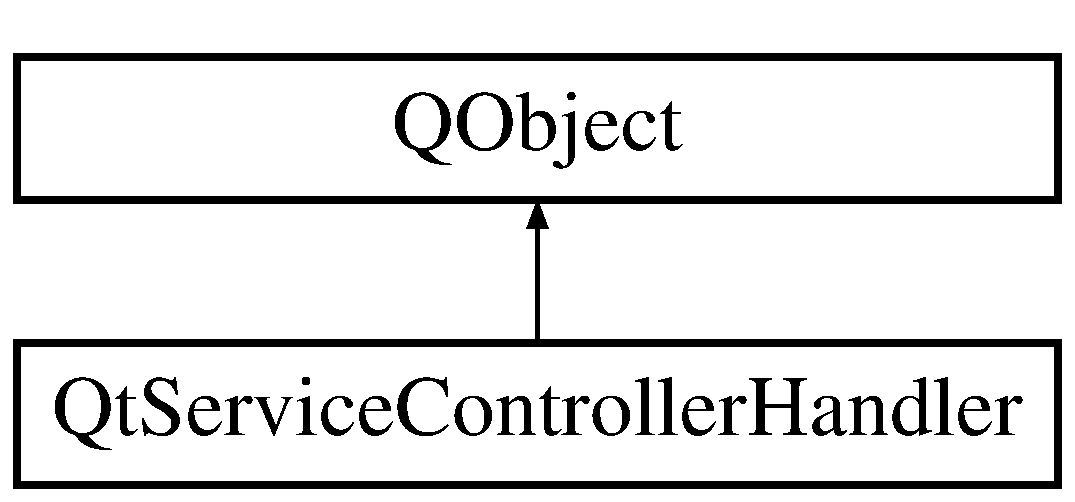
\includegraphics[height=2.000000cm]{class_qt_service_controller_handler}
\end{center}
\end{figure}
\subsection*{Public Member Functions}
\begin{DoxyCompactItemize}
\item 
\mbox{\Hypertarget{class_qt_service_controller_handler_aececaafe4c1381e632ff5da78187d136}\label{class_qt_service_controller_handler_aececaafe4c1381e632ff5da78187d136}} 
{\bfseries Qt\+Service\+Controller\+Handler} (\hyperlink{class_qt_service_sys_private}{Qt\+Service\+Sys\+Private} $\ast$sys)
\end{DoxyCompactItemize}
\subsection*{Protected Member Functions}
\begin{DoxyCompactItemize}
\item 
\mbox{\Hypertarget{class_qt_service_controller_handler_a92e2fafac640400c4defe718024f5340}\label{class_qt_service_controller_handler_a92e2fafac640400c4defe718024f5340}} 
void {\bfseries custom\+Event} (Q\+Event $\ast$e)
\end{DoxyCompactItemize}


The documentation for this class was generated from the following file\+:\begin{DoxyCompactItemize}
\item 
L\+C\+S\+Server/\+Qt\+Solutions\+Service/src/qtservice\+\_\+win.\+cpp\end{DoxyCompactItemize}

\hypertarget{class_qt_service_controller_private}{}\section{Qt\+Service\+Controller\+Private Class Reference}
\label{class_qt_service_controller_private}\index{Qt\+Service\+Controller\+Private@{Qt\+Service\+Controller\+Private}}
\subsection*{Public Attributes}
\begin{DoxyCompactItemize}
\item 
\mbox{\Hypertarget{class_qt_service_controller_private_ab0c1b3e4f6189e131073b85d869a9823}\label{class_qt_service_controller_private_ab0c1b3e4f6189e131073b85d869a9823}} 
Q\+String {\bfseries service\+Name}
\item 
\mbox{\Hypertarget{class_qt_service_controller_private_ac02268c462ca6440fddb3c319639da11}\label{class_qt_service_controller_private_ac02268c462ca6440fddb3c319639da11}} 
\hyperlink{class_qt_service_controller}{Qt\+Service\+Controller} $\ast$ {\bfseries q\+\_\+ptr}
\end{DoxyCompactItemize}


The documentation for this class was generated from the following file\+:\begin{DoxyCompactItemize}
\item 
L\+C\+S\+Server/\+Qt\+Solutions\+Service/src/qtservice\+\_\+p.\+h\end{DoxyCompactItemize}

\hypertarget{class_qt_service_starter}{}\section{Qt\+Service\+Starter Class Reference}
\label{class_qt_service_starter}\index{Qt\+Service\+Starter@{Qt\+Service\+Starter}}
Inheritance diagram for Qt\+Service\+Starter\+:\begin{figure}[H]
\begin{center}
\leavevmode
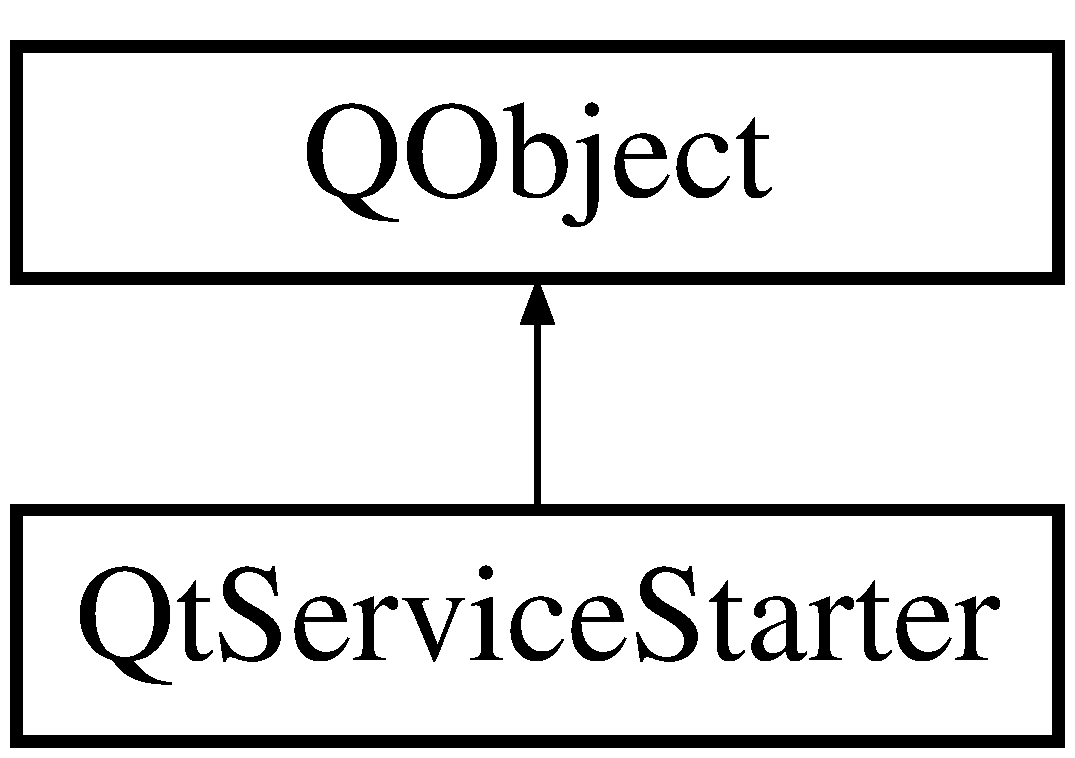
\includegraphics[height=2.000000cm]{class_qt_service_starter}
\end{center}
\end{figure}
\subsection*{Public Slots}
\begin{DoxyCompactItemize}
\item 
\mbox{\Hypertarget{class_qt_service_starter_adfd8ef0a999b55ca6eeefafee52cf8dc}\label{class_qt_service_starter_adfd8ef0a999b55ca6eeefafee52cf8dc}} 
void {\bfseries slot\+Start} ()
\end{DoxyCompactItemize}
\subsection*{Public Member Functions}
\begin{DoxyCompactItemize}
\item 
\mbox{\Hypertarget{class_qt_service_starter_ac192dd9044e8ff6a663a456d88e16fdc}\label{class_qt_service_starter_ac192dd9044e8ff6a663a456d88e16fdc}} 
{\bfseries Qt\+Service\+Starter} (\hyperlink{class_qt_service_base_private}{Qt\+Service\+Base\+Private} $\ast$service)
\end{DoxyCompactItemize}


The documentation for this class was generated from the following file\+:\begin{DoxyCompactItemize}
\item 
L\+C\+S\+Server/\+Qt\+Solutions\+Service/src/qtservice.\+cpp\end{DoxyCompactItemize}

\hypertarget{class_qt_service_sys_private}{}\section{Qt\+Service\+Sys\+Private Class Reference}
\label{class_qt_service_sys_private}\index{Qt\+Service\+Sys\+Private@{Qt\+Service\+Sys\+Private}}
Inheritance diagram for Qt\+Service\+Sys\+Private\+:\begin{figure}[H]
\begin{center}
\leavevmode
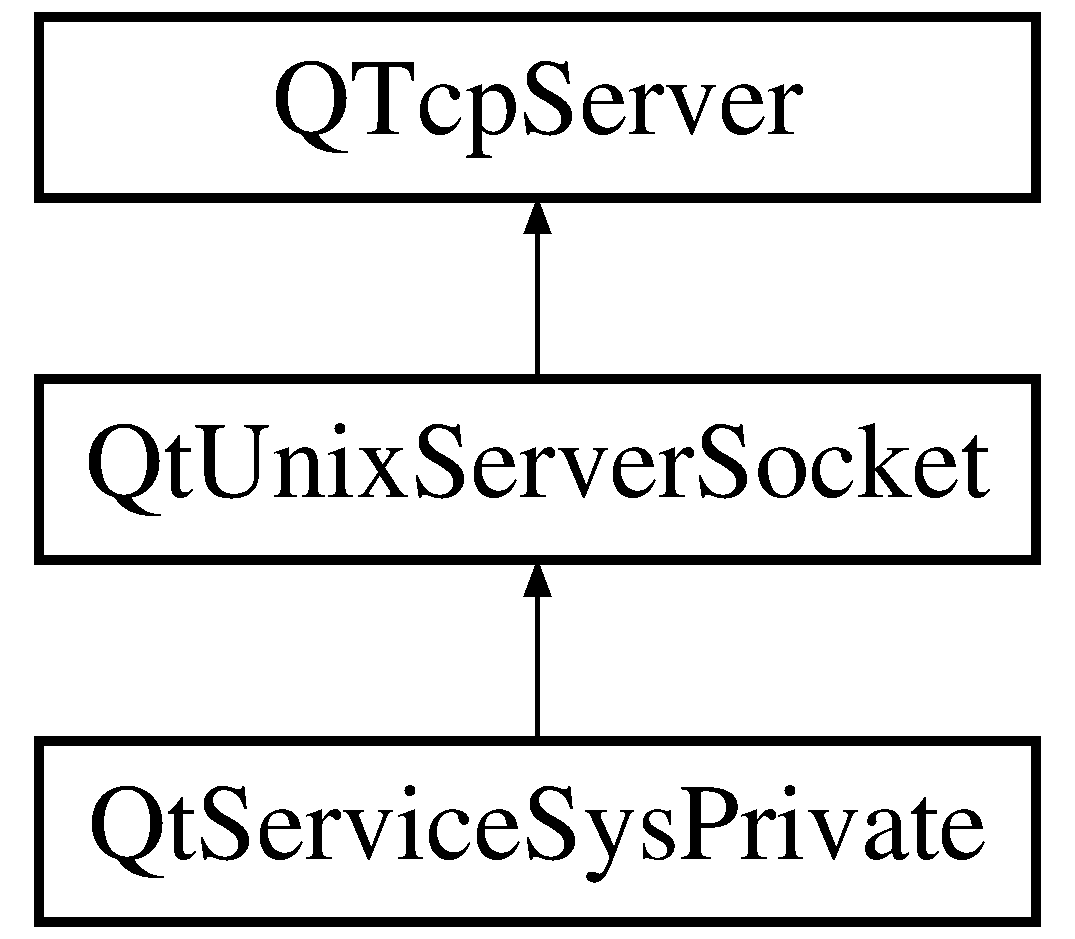
\includegraphics[height=3.000000cm]{class_qt_service_sys_private}
\end{center}
\end{figure}
\subsection*{Public Types}
\begin{DoxyCompactItemize}
\item 
\mbox{\Hypertarget{class_qt_service_sys_private_af1a08fe54ff9ccc14463eb7ae4089257}\label{class_qt_service_sys_private_af1a08fe54ff9ccc14463eb7ae4089257}} 
enum \{ {\bfseries Q\+T\+S\+E\+R\+V\+I\+C\+E\+\_\+\+S\+T\+A\+R\+T\+UP} = 256
 \}
\end{DoxyCompactItemize}
\subsection*{Public Member Functions}
\begin{DoxyCompactItemize}
\item 
\mbox{\Hypertarget{class_qt_service_sys_private_a1d33416e766b6f475d36038467bdd69a}\label{class_qt_service_sys_private_a1d33416e766b6f475d36038467bdd69a}} 
void {\bfseries set\+Status} (D\+W\+O\+RD dw\+State)
\item 
\mbox{\Hypertarget{class_qt_service_sys_private_a8d9929e1406f32ac3f71446ab86d0577}\label{class_qt_service_sys_private_a8d9929e1406f32ac3f71446ab86d0577}} 
void {\bfseries set\+Service\+Flags} (Qt\+Service\+Base\+::\+Service\+Flags flags)
\item 
\mbox{\Hypertarget{class_qt_service_sys_private_a8951a293950f651468b69ba142afe017}\label{class_qt_service_sys_private_a8951a293950f651468b69ba142afe017}} 
D\+W\+O\+RD {\bfseries service\+Flags} (Qt\+Service\+Base\+::\+Service\+Flags flags) const
\item 
\mbox{\Hypertarget{class_qt_service_sys_private_ab023c74e63bc134ff13495891e34f385}\label{class_qt_service_sys_private_ab023c74e63bc134ff13495891e34f385}} 
bool {\bfseries available} () const
\item 
\mbox{\Hypertarget{class_qt_service_sys_private_aeb0603830564cf6d730549866020bf0a}\label{class_qt_service_sys_private_aeb0603830564cf6d730549866020bf0a}} 
void {\bfseries handle\+Custom\+Event} (Q\+Event $\ast$e)
\end{DoxyCompactItemize}
\subsection*{Static Public Member Functions}
\begin{DoxyCompactItemize}
\item 
\mbox{\Hypertarget{class_qt_service_sys_private_a0ebf25dd25c87974b313c79b696aec6e}\label{class_qt_service_sys_private_a0ebf25dd25c87974b313c79b696aec6e}} 
static void W\+I\+N\+A\+PI {\bfseries service\+Main} (D\+W\+O\+RD dw\+Argc, wchar\+\_\+t $\ast$$\ast$lpsz\+Argv)
\item 
\mbox{\Hypertarget{class_qt_service_sys_private_abec91d93c5a6562dfac877e4074c24d2}\label{class_qt_service_sys_private_abec91d93c5a6562dfac877e4074c24d2}} 
static void W\+I\+N\+A\+PI {\bfseries handler} (D\+W\+O\+RD dw\+Opcode)
\end{DoxyCompactItemize}
\subsection*{Public Attributes}
\begin{DoxyCompactItemize}
\item 
\mbox{\Hypertarget{class_qt_service_sys_private_a5b718dc890ba28a1a8ecc2c292ed3683}\label{class_qt_service_sys_private_a5b718dc890ba28a1a8ecc2c292ed3683}} 
char $\ast$ {\bfseries ident}
\item 
\mbox{\Hypertarget{class_qt_service_sys_private_ab3a1a34e95b1028d2d2437ce5683ce25}\label{class_qt_service_sys_private_ab3a1a34e95b1028d2d2437ce5683ce25}} 
Qt\+Service\+Base\+::\+Service\+Flags {\bfseries service\+Flags}
\item 
\mbox{\Hypertarget{class_qt_service_sys_private_a4eaa8c9fb344d5fcbe52e13d9b563749}\label{class_qt_service_sys_private_a4eaa8c9fb344d5fcbe52e13d9b563749}} 
S\+E\+R\+V\+I\+C\+E\+\_\+\+S\+T\+A\+T\+US {\bfseries status}
\item 
\mbox{\Hypertarget{class_qt_service_sys_private_a5794a5ac189b478c944426805b41ae2c}\label{class_qt_service_sys_private_a5794a5ac189b478c944426805b41ae2c}} 
S\+E\+R\+V\+I\+C\+E\+\_\+\+S\+T\+A\+T\+U\+S\+\_\+\+H\+A\+N\+D\+LE {\bfseries service\+Status}
\item 
\mbox{\Hypertarget{class_qt_service_sys_private_aece0e34030f5abf3ec7bee64b4ab22a3}\label{class_qt_service_sys_private_aece0e34030f5abf3ec7bee64b4ab22a3}} 
Q\+String\+List {\bfseries service\+Args}
\item 
\mbox{\Hypertarget{class_qt_service_sys_private_a8fc09bc3f805b5afe18e5d2a5d42f466}\label{class_qt_service_sys_private_a8fc09bc3f805b5afe18e5d2a5d42f466}} 
Q\+Wait\+Condition {\bfseries condition}
\item 
\mbox{\Hypertarget{class_qt_service_sys_private_a13840c7d50506cea8ac099d75ed5bd94}\label{class_qt_service_sys_private_a13840c7d50506cea8ac099d75ed5bd94}} 
Q\+Mutex {\bfseries mutex}
\item 
\mbox{\Hypertarget{class_qt_service_sys_private_a2b96b9ff0db26655accab99d6527fe3d}\label{class_qt_service_sys_private_a2b96b9ff0db26655accab99d6527fe3d}} 
Q\+Semaphore {\bfseries start\+Semaphore}
\item 
\mbox{\Hypertarget{class_qt_service_sys_private_ab81c4cc12732b32d6962253868fde059}\label{class_qt_service_sys_private_ab81c4cc12732b32d6962253868fde059}} 
Q\+Semaphore {\bfseries start\+Semaphore2}
\item 
\mbox{\Hypertarget{class_qt_service_sys_private_ac8834f0ad3dd97b1dfb9e7de563ee5cb}\label{class_qt_service_sys_private_ac8834f0ad3dd97b1dfb9e7de563ee5cb}} 
\hyperlink{class_qt_service_controller_handler}{Qt\+Service\+Controller\+Handler} $\ast$ {\bfseries controller\+Handler}
\end{DoxyCompactItemize}
\subsection*{Static Public Attributes}
\begin{DoxyCompactItemize}
\item 
\mbox{\Hypertarget{class_qt_service_sys_private_a1c67be022e972d4e1f7d9aad91464222}\label{class_qt_service_sys_private_a1c67be022e972d4e1f7d9aad91464222}} 
static \hyperlink{class_qt_service_sys_private}{Qt\+Service\+Sys\+Private} $\ast$ {\bfseries instance} = 0
\item 
\mbox{\Hypertarget{class_qt_service_sys_private_aeb77807c5daf3c8f1386ffec7a9157c7}\label{class_qt_service_sys_private_aeb77807c5daf3c8f1386ffec7a9157c7}} 
static Q\+Core\+Application\+::\+Event\+Filter {\bfseries next\+Filter} = 0
\end{DoxyCompactItemize}
\subsection*{Protected Member Functions}
\begin{DoxyCompactItemize}
\item 
\mbox{\Hypertarget{class_qt_service_sys_private_aef4490778cdd725fe8a76839e4afe86a}\label{class_qt_service_sys_private_aef4490778cdd725fe8a76839e4afe86a}} 
void {\bfseries incoming\+Connection} (int socket\+Descriptor)
\end{DoxyCompactItemize}


The documentation for this class was generated from the following files\+:\begin{DoxyCompactItemize}
\item 
L\+C\+S\+Server/\+Qt\+Solutions\+Service/src/qtservice\+\_\+unix.\+cpp\item 
L\+C\+S\+Server/\+Qt\+Solutions\+Service/src/qtservice\+\_\+win.\+cpp\end{DoxyCompactItemize}

\hypertarget{class_qt_unix_server_socket}{}\section{Qt\+Unix\+Server\+Socket Class Reference}
\label{class_qt_unix_server_socket}\index{Qt\+Unix\+Server\+Socket@{Qt\+Unix\+Server\+Socket}}
Inheritance diagram for Qt\+Unix\+Server\+Socket\+:\begin{figure}[H]
\begin{center}
\leavevmode
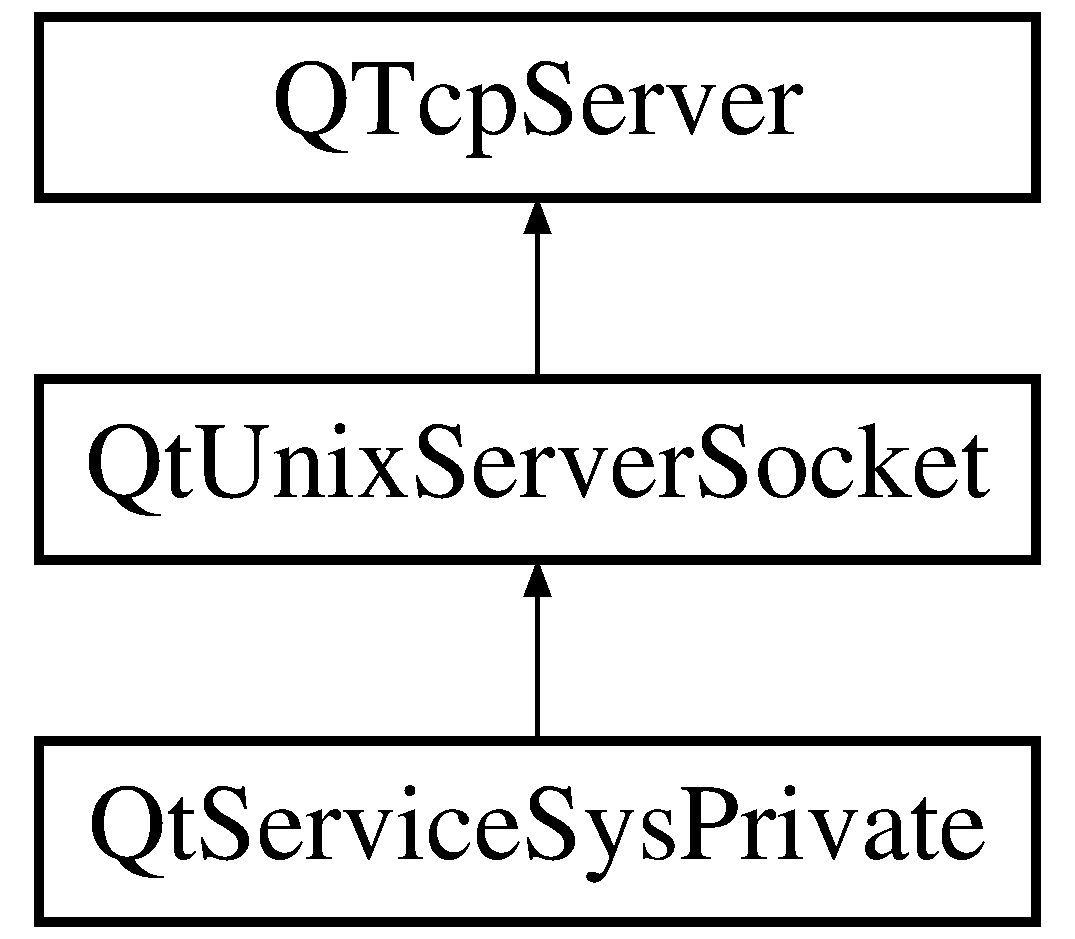
\includegraphics[height=3.000000cm]{class_qt_unix_server_socket}
\end{center}
\end{figure}
\subsection*{Public Member Functions}
\begin{DoxyCompactItemize}
\item 
\mbox{\Hypertarget{class_qt_unix_server_socket_a9b6133aa5f66a9acf58529cdf865efe4}\label{class_qt_unix_server_socket_a9b6133aa5f66a9acf58529cdf865efe4}} 
{\bfseries Qt\+Unix\+Server\+Socket} (const Q\+String \&path, Q\+Object $\ast$parent=0)
\item 
\mbox{\Hypertarget{class_qt_unix_server_socket_aa73dd123bc2ff7a7a90eb408fce90194}\label{class_qt_unix_server_socket_aa73dd123bc2ff7a7a90eb408fce90194}} 
{\bfseries Qt\+Unix\+Server\+Socket} (Q\+Object $\ast$parent=0)
\item 
\mbox{\Hypertarget{class_qt_unix_server_socket_a733cf66cddbbf31d8a37675f349d2ca8}\label{class_qt_unix_server_socket_a733cf66cddbbf31d8a37675f349d2ca8}} 
void {\bfseries set\+Path} (const Q\+String \&path)
\item 
\mbox{\Hypertarget{class_qt_unix_server_socket_a74bdb3e24b99bb55d7101651a2e86205}\label{class_qt_unix_server_socket_a74bdb3e24b99bb55d7101651a2e86205}} 
void {\bfseries close} ()
\end{DoxyCompactItemize}


The documentation for this class was generated from the following files\+:\begin{DoxyCompactItemize}
\item 
L\+C\+S\+Server/\+Qt\+Solutions\+Service/src/qtunixserversocket.\+h\item 
L\+C\+S\+Server/\+Qt\+Solutions\+Service/src/qtunixserversocket.\+cpp\end{DoxyCompactItemize}

\hypertarget{class_qt_unix_socket}{}\section{Qt\+Unix\+Socket Class Reference}
\label{class_qt_unix_socket}\index{Qt\+Unix\+Socket@{Qt\+Unix\+Socket}}
Inheritance diagram for Qt\+Unix\+Socket\+:\begin{figure}[H]
\begin{center}
\leavevmode
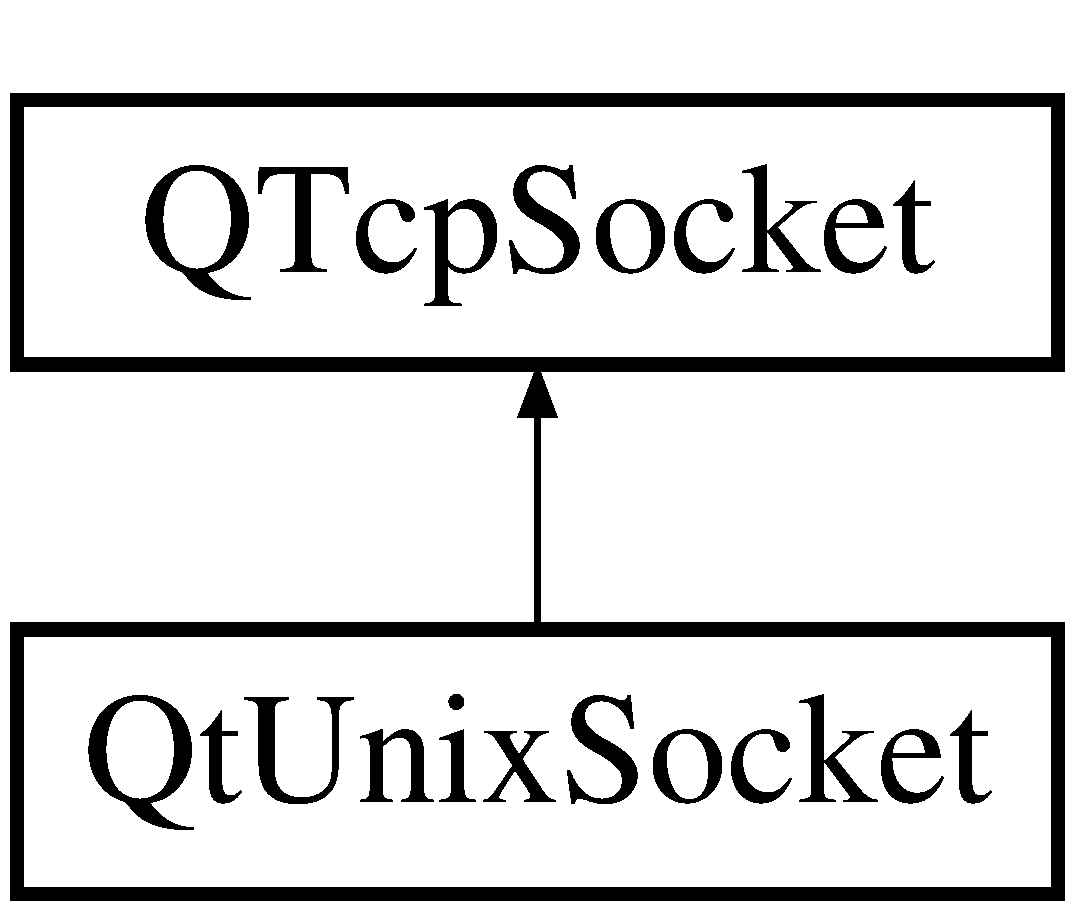
\includegraphics[height=2.000000cm]{class_qt_unix_socket}
\end{center}
\end{figure}
\subsection*{Public Member Functions}
\begin{DoxyCompactItemize}
\item 
\mbox{\Hypertarget{class_qt_unix_socket_a5c8729be0bb51069bc5011c131a3c396}\label{class_qt_unix_socket_a5c8729be0bb51069bc5011c131a3c396}} 
{\bfseries Qt\+Unix\+Socket} (Q\+Object $\ast$parent=0)
\item 
\mbox{\Hypertarget{class_qt_unix_socket_a412e4407c955f2cfceabdae69f1626ff}\label{class_qt_unix_socket_a412e4407c955f2cfceabdae69f1626ff}} 
bool {\bfseries connect\+To} (const Q\+String \&path)
\end{DoxyCompactItemize}


The documentation for this class was generated from the following files\+:\begin{DoxyCompactItemize}
\item 
L\+C\+S\+Server/\+Qt\+Solutions\+Service/src/qtunixsocket.\+h\item 
L\+C\+S\+Server/\+Qt\+Solutions\+Service/src/qtunixsocket.\+cpp\end{DoxyCompactItemize}

\hypertarget{class_serial_port_thread}{}\section{Serial\+Port\+Thread Class Reference}
\label{class_serial_port_thread}\index{Serial\+Port\+Thread@{Serial\+Port\+Thread}}
Inheritance diagram for Serial\+Port\+Thread\+:\begin{figure}[H]
\begin{center}
\leavevmode
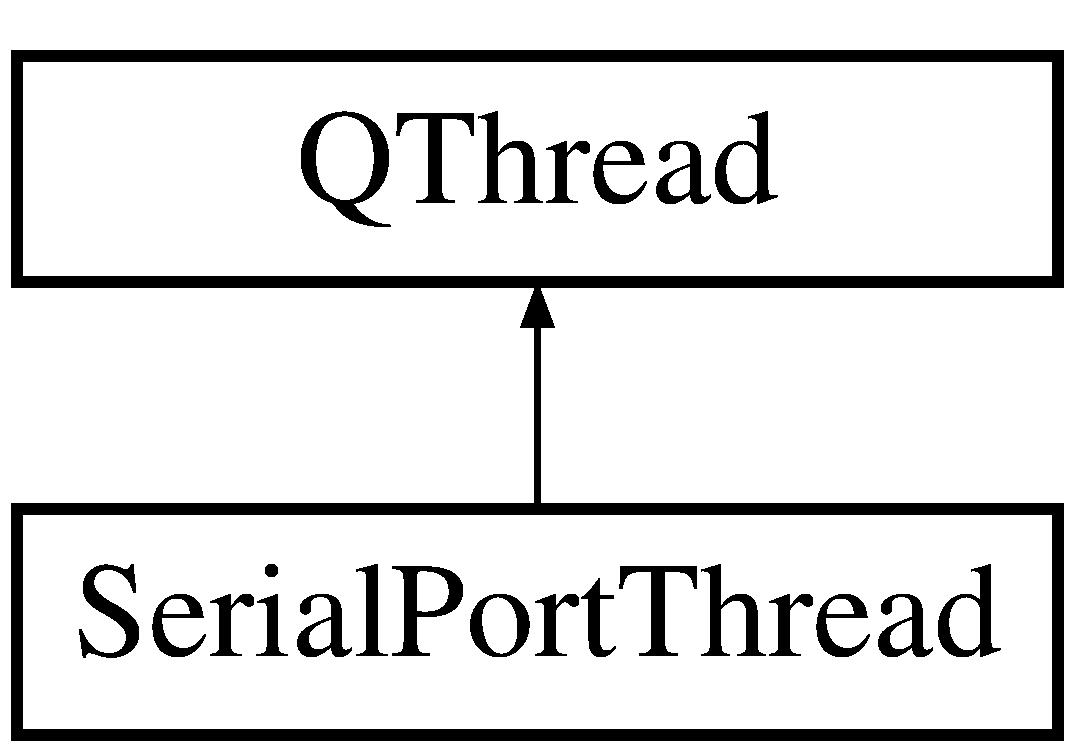
\includegraphics[height=2.000000cm]{class_serial_port_thread}
\end{center}
\end{figure}
\subsection*{Public Types}
\begin{DoxyCompactItemize}
\item 
\mbox{\Hypertarget{class_serial_port_thread_a2a5f36babceca39d2b8698c9a02d93e2}\label{class_serial_port_thread_a2a5f36babceca39d2b8698c9a02d93e2}} 
enum {\bfseries Port\+Status\+Enum} \{ {\bfseries Disconnected}, 
{\bfseries Connected}, 
{\bfseries Running}
 \}
\end{DoxyCompactItemize}
\subsection*{Public Slots}
\begin{DoxyCompactItemize}
\item 
\mbox{\Hypertarget{class_serial_port_thread_ae69ad77b0a8efd9652ddc249a61565f4}\label{class_serial_port_thread_ae69ad77b0a8efd9652ddc249a61565f4}} 
void {\bfseries send\+Message} (const \hyperlink{class_n_c_e_message}{N\+C\+E\+Message} \&message)
\item 
\mbox{\Hypertarget{class_serial_port_thread_a90726304c2d0fb01e1519b3ec606164c}\label{class_serial_port_thread_a90726304c2d0fb01e1519b3ec606164c}} 
void {\bfseries poll\+Command\+Station} (void)
\end{DoxyCompactItemize}
\subsection*{Signals}
\begin{DoxyCompactItemize}
\item 
\mbox{\Hypertarget{class_serial_port_thread_afd82dc4692e9acd7b25444b357243688}\label{class_serial_port_thread_afd82dc4692e9acd7b25444b357243688}} 
void {\bfseries new\+Message} (const \hyperlink{class_n_c_e_message}{N\+C\+E\+Message} \&message)
\item 
\mbox{\Hypertarget{class_serial_port_thread_a9915b851f045269a962a23a53cbd70ce}\label{class_serial_port_thread_a9915b851f045269a962a23a53cbd70ce}} 
void {\bfseries buffer\+Initialized} (void)
\item 
\mbox{\Hypertarget{class_serial_port_thread_aa854a362aa5610ec12ccb9c670c09ee1}\label{class_serial_port_thread_aa854a362aa5610ec12ccb9c670c09ee1}} 
void {\bfseries buffer\+Data\+Changed} (quint8 byte, int block\+Index, int byte\+Index)
\end{DoxyCompactItemize}
\subsection*{Public Member Functions}
\begin{DoxyCompactItemize}
\item 
\mbox{\Hypertarget{class_serial_port_thread_a5dc5088f166705325cc4a4215410b48b}\label{class_serial_port_thread_a5dc5088f166705325cc4a4215410b48b}} 
\hyperlink{class_serial_port_thread_a5dc5088f166705325cc4a4215410b48b}{Serial\+Port\+Thread} (Q\+Object $\ast$parent)
\begin{DoxyCompactList}\small\item\em \hyperlink{class_serial_port_thread}{Serial\+Port\+Thread}. \end{DoxyCompactList}\item 
\mbox{\Hypertarget{class_serial_port_thread_a8cb6df223cc54a75e2f6f2f8a87ad1be}\label{class_serial_port_thread_a8cb6df223cc54a75e2f6f2f8a87ad1be}} 
virtual void {\bfseries run} (void) Q\+\_\+\+D\+E\+C\+L\+\_\+\+O\+V\+E\+R\+R\+I\+DE
\item 
\mbox{\Hypertarget{class_serial_port_thread_af995d293c19c8b18e8bdb0e5b99dd6bb}\label{class_serial_port_thread_af995d293c19c8b18e8bdb0e5b99dd6bb}} 
void {\bfseries set\+Quit} (void)
\item 
\mbox{\Hypertarget{class_serial_port_thread_a71b5db795c9ffb96071afc4a2a8c71ba}\label{class_serial_port_thread_a71b5db795c9ffb96071afc4a2a8c71ba}} 
void {\bfseries open\+Port} (void)
\end{DoxyCompactItemize}


The documentation for this class was generated from the following files\+:\begin{DoxyCompactItemize}
\item 
L\+C\+S\+Server/N\+C\+E\+Interface.\+h\item 
L\+C\+S\+Server/N\+C\+E\+Interface.\+cpp\end{DoxyCompactItemize}

\hypertarget{class_simulator}{}\section{Simulator Class Reference}
\label{class_simulator}\index{Simulator@{Simulator}}
Inheritance diagram for Simulator\+:\begin{figure}[H]
\begin{center}
\leavevmode
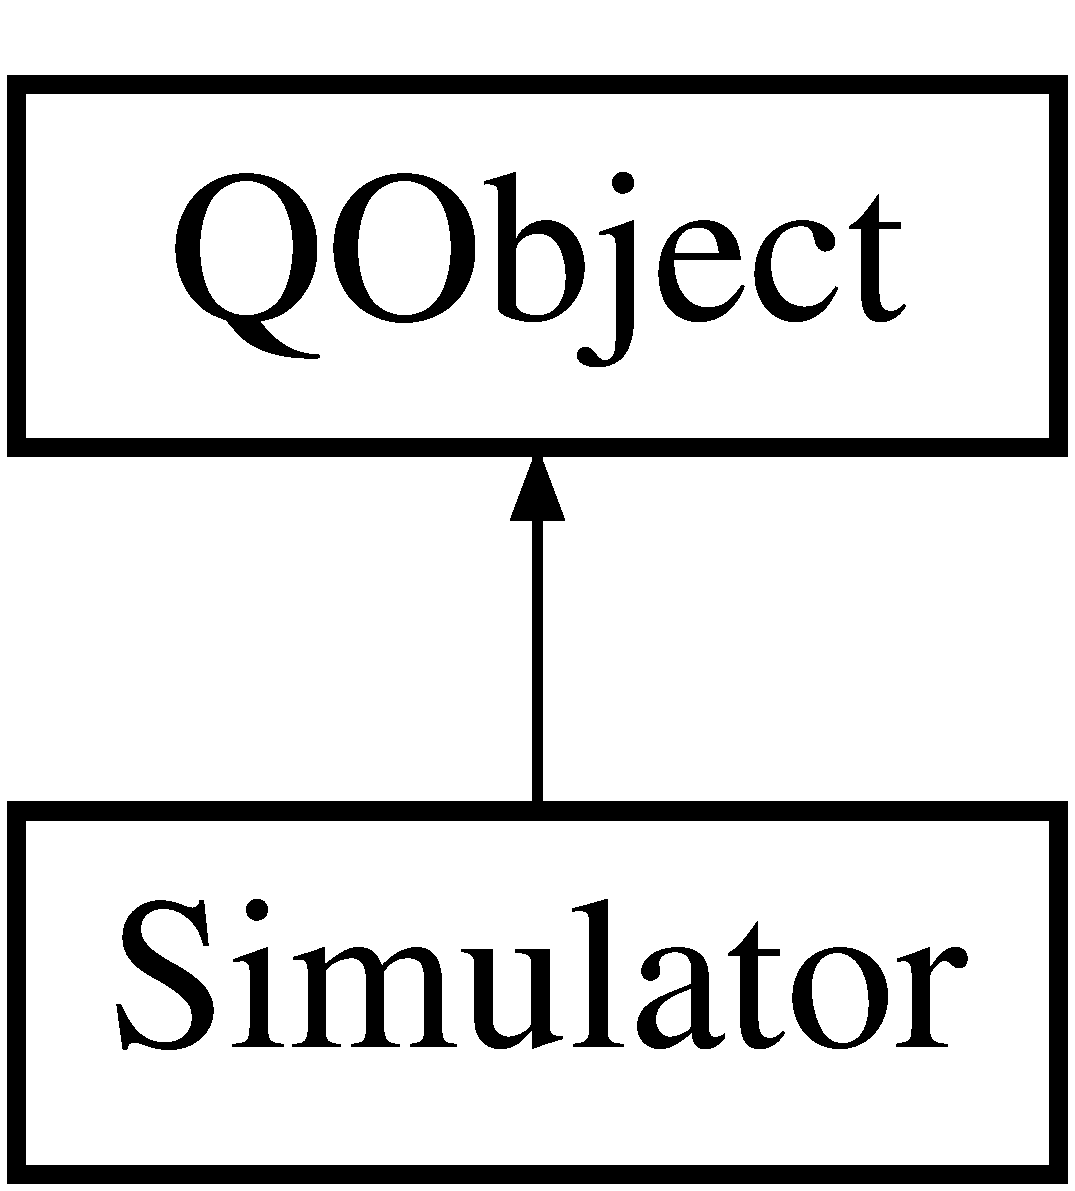
\includegraphics[height=2.000000cm]{class_simulator}
\end{center}
\end{figure}
\subsection*{Public Slots}
\begin{DoxyCompactItemize}
\item 
\mbox{\Hypertarget{class_simulator_a78a01e50374bc7f7c48d5c0844c0c553}\label{class_simulator_a78a01e50374bc7f7c48d5c0844c0c553}} 
void {\bfseries new\+Message} (const \hyperlink{class_u_d_p_message}{U\+D\+P\+Message} \&message)
\item 
\mbox{\Hypertarget{class_simulator_a17d6e27215aa41041477d849a2056e40}\label{class_simulator_a17d6e27215aa41041477d849a2056e40}} 
void {\bfseries timer\+Proc} (void)
\end{DoxyCompactItemize}
\subsection*{Public Member Functions}
\begin{DoxyCompactItemize}
\item 
\mbox{\Hypertarget{class_simulator_aa10d08136ea5bde785d46d8eb62fb4cf}\label{class_simulator_aa10d08136ea5bde785d46d8eb62fb4cf}} 
{\bfseries Simulator} (Q\+Object $\ast$parent=nullptr)
\end{DoxyCompactItemize}


The documentation for this class was generated from the following files\+:\begin{DoxyCompactItemize}
\item 
L\+C\+S\+Server/Simulator.\+h\item 
L\+C\+S\+Server/Simulator.\+cpp\end{DoxyCompactItemize}

\hypertarget{class_status_dialog}{}\section{Status\+Dialog Class Reference}
\label{class_status_dialog}\index{Status\+Dialog@{Status\+Dialog}}
Inheritance diagram for Status\+Dialog\+:\begin{figure}[H]
\begin{center}
\leavevmode
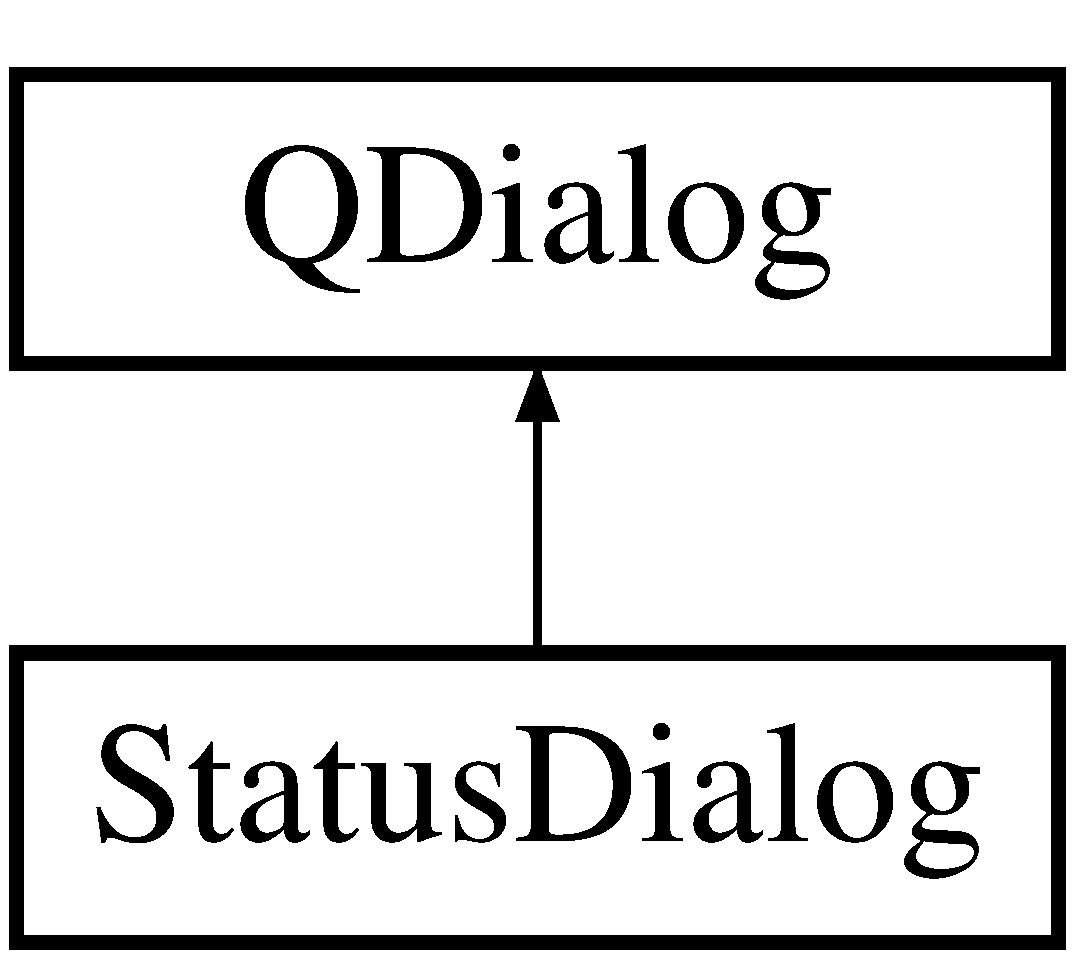
\includegraphics[height=2.000000cm]{class_status_dialog}
\end{center}
\end{figure}
\subsection*{Public Member Functions}
\begin{DoxyCompactItemize}
\item 
\mbox{\Hypertarget{class_status_dialog_a814831672ff09b7e3c03b61e25fe7a5d}\label{class_status_dialog_a814831672ff09b7e3c03b61e25fe7a5d}} 
{\bfseries Status\+Dialog} (Q\+Widget $\ast$parent=0)
\end{DoxyCompactItemize}
\subsection*{Protected Slots}
\begin{DoxyCompactItemize}
\item 
\mbox{\Hypertarget{class_status_dialog_a070ec51a69f12ddc1f8ee2a89572653b}\label{class_status_dialog_a070ec51a69f12ddc1f8ee2a89572653b}} 
void {\bfseries on\+Controller\+Connected} (int index)
\item 
\mbox{\Hypertarget{class_status_dialog_ac40b32574e672937d93721699d5c6fe6}\label{class_status_dialog_ac40b32574e672937d93721699d5c6fe6}} 
void {\bfseries on\+Controller\+Disconnected} (int index)
\item 
\mbox{\Hypertarget{class_status_dialog_a9dd8cc9ccc2786d50ac5ac2c3ff46253}\label{class_status_dialog_a9dd8cc9ccc2786d50ac5ac2c3ff46253}} 
void {\bfseries on\+Controller\+Ping} (int index, quint64 length)
\item 
\mbox{\Hypertarget{class_status_dialog_a09e16d6a6e98ad4088b261ee2692f1ae}\label{class_status_dialog_a09e16d6a6e98ad4088b261ee2692f1ae}} 
void {\bfseries on\+Device\+Status\+Changed} (int device\+ID, int status)
\item 
\mbox{\Hypertarget{class_status_dialog_a97af838c425027913920559f9e4e3bfe}\label{class_status_dialog_a97af838c425027913920559f9e4e3bfe}} 
void {\bfseries on\+Pin\+State\+Changed} (int address, int pin\+Number, int pin\+Mode)
\item 
\mbox{\Hypertarget{class_status_dialog_a750b9f3c081f4e04c7981a42915168be}\label{class_status_dialog_a750b9f3c081f4e04c7981a42915168be}} 
void {\bfseries on\+N\+C\+E\+Data\+Changed} (quint8 data, int block\+Index, int byte\+Index)
\end{DoxyCompactItemize}


The documentation for this class was generated from the following files\+:\begin{DoxyCompactItemize}
\item 
L\+C\+S\+Server/Status\+Dialog.\+h\item 
L\+C\+S\+Server/Status\+Dialog.\+cpp\end{DoxyCompactItemize}

\hypertarget{class_u_d_p_message}{}\section{U\+D\+P\+Message Class Reference}
\label{class_u_d_p_message}\index{U\+D\+P\+Message@{U\+D\+P\+Message}}


A class for handling U\+DP messages sent between controllers and the application server.  




{\ttfamily \#include $<$U\+D\+P\+Message.\+h$>$}

\subsection*{Public Member Functions}
\begin{DoxyCompactItemize}
\item 
\hyperlink{class_u_d_p_message_a823351519fc5818ccc03030c6947e620}{U\+D\+P\+Message} (void)
\item 
\hyperlink{class_u_d_p_message_adbc0139ef0249efd4a932bbc0b57fe13}{U\+D\+P\+Message} (const \hyperlink{class_u_d_p_message}{U\+D\+P\+Message} \&other)
\item 
\hyperlink{class_u_d_p_message_a6edf87f4f8f441edf2064d5f6fa5cd02}{U\+D\+P\+Message} (const \hyperlink{struct_u_d_p_message_struct}{U\+D\+P\+Message\+Struct} \&other)
\item 
\hyperlink{class_u_d_p_message}{U\+D\+P\+Message} \& \hyperlink{class_u_d_p_message_af3bb7f16fec948bcfbf99646b79c5c58}{operator=} (const \hyperlink{class_u_d_p_message}{U\+D\+P\+Message} \&other)
\item 
\mbox{\Hypertarget{class_u_d_p_message_ad732ecdc07825ce944b251b0e8f55e90}\label{class_u_d_p_message_ad732ecdc07825ce944b251b0e8f55e90}} 
bool \hyperlink{class_u_d_p_message_ad732ecdc07825ce944b251b0e8f55e90}{is\+Valid} (void) const
\begin{DoxyCompactList}\small\item\em Returns true if the message is considered valid. At minimum, a valid message has its message ID set to a value greater than zero. \end{DoxyCompactList}\item 
void \hyperlink{class_u_d_p_message_aba4aadebe7b1aa92ba558f3cd4319e79}{set\+Message\+ID} (unsigned char value)
\item 
void \hyperlink{class_u_d_p_message_a2fcacc64fbb5598848a391c9fd9aa8c2}{set\+ID} (long value)
\item 
void \hyperlink{class_u_d_p_message_ad7f1c729cf357be18e6cda695f5e5d99}{set\+Field} (unsigned char field\+Index, unsigned char value)
\item 
\mbox{\Hypertarget{class_u_d_p_message_aeea2288e53b4c6db7861181b5fc8aa5e}\label{class_u_d_p_message_aeea2288e53b4c6db7861181b5fc8aa5e}} 
char $\ast$ \hyperlink{class_u_d_p_message_aeea2288e53b4c6db7861181b5fc8aa5e}{get\+Ref} (void) const
\begin{DoxyCompactList}\small\item\em returns a reference to the internal \hyperlink{struct_u_d_p_message_struct}{U\+D\+P\+Message\+Struct} \end{DoxyCompactList}\item 
\mbox{\Hypertarget{class_u_d_p_message_a9e762f6c16fa298afe87b9dd6cee41c2}\label{class_u_d_p_message_a9e762f6c16fa298afe87b9dd6cee41c2}} 
unsigned char \hyperlink{class_u_d_p_message_a9e762f6c16fa298afe87b9dd6cee41c2}{get\+Message\+ID} (void) const
\begin{DoxyCompactList}\small\item\em returns the message\+ID. \end{DoxyCompactList}\item 
\mbox{\Hypertarget{class_u_d_p_message_add45e9751d72e7d789ed6dcdb06c23d2}\label{class_u_d_p_message_add45e9751d72e7d789ed6dcdb06c23d2}} 
long \hyperlink{class_u_d_p_message_add45e9751d72e7d789ed6dcdb06c23d2}{get\+ID} (void) const
\begin{DoxyCompactList}\small\item\em returns the ID \end{DoxyCompactList}\item 
\mbox{\Hypertarget{class_u_d_p_message_a65fed9ee9c6dc936e1c9d1ae3052d1f7}\label{class_u_d_p_message_a65fed9ee9c6dc936e1c9d1ae3052d1f7}} 
unsigned char \hyperlink{class_u_d_p_message_a65fed9ee9c6dc936e1c9d1ae3052d1f7}{get\+Transaction\+Number} (void) const
\begin{DoxyCompactList}\small\item\em returns the transaction number \end{DoxyCompactList}\item 
void \hyperlink{class_u_d_p_message_a27629d5cab43160d53cedfd894e1c216}{set\+Transaction\+Number} (unsigned char value)
\item 
unsigned char \hyperlink{class_u_d_p_message_a869585e0916d3b9edf99111f8fc74709}{get\+Field} (unsigned char field\+Index) const
\item 
void \hyperlink{class_u_d_p_message_a313c116a2f7f0f134745ed0c4a759733}{copy\+From} (const \hyperlink{class_u_d_p_message}{U\+D\+P\+Message} \&other)
\end{DoxyCompactItemize}


\subsection{Detailed Description}
A class for handling U\+DP messages sent between controllers and the application server. 

\hyperlink{class_u_d_p_message}{U\+D\+P\+Message} This class along with the \hyperlink{struct_u_d_p_message_struct}{Message Structure} contains the data layout of a U\+DP message. Messages are sent from controller-\/to-\/controller in a peer-\/to-\/peer fasion using U\+DP uni-\/cast. Each controller contains a list of \char`\"{}controllers to notify\char`\"{} in its configuration data. Each time a device needs to send a command or status message, the controller\textquotesingle{}s Network Manager sends the message to all controllers contained in the notification list. Each controller listens for the \hyperlink{group___u_d_p_message_i_d_ga23aab89076591390a1dbc412a3a07314}{S\+Y\+S\+\_\+\+C\+O\+N\+T\+R\+O\+L\+L\+E\+R\+\_\+\+O\+N\+L\+I\+NE} broadcast message which is sent by each controller upon startup. Upon resceiving this message, the controller checks to see if the controller\textquotesingle{}s ID is contained in its notification list and, if so, stores the address of the sending controller which is stored in field\mbox{[}0\mbox{]} -\/ field\mbox{[}3\mbox{]} and then responds by sending device status messages. If the controller misses this message, the controller sends a \hyperlink{group___u_d_p_message_i_d_gadfda0e5a5a6a08de555dd55182a4cd87}{S\+Y\+S\+\_\+\+F\+I\+N\+D\+\_\+\+C\+O\+N\+T\+R\+O\+L\+L\+ER} broadcast message every 3 seconds for each controller in its notification list until it recieves a corresponding \hyperlink{group___u_d_p_message_i_d_ga23aab89076591390a1dbc412a3a07314}{S\+Y\+S\+\_\+\+C\+O\+N\+T\+R\+O\+L\+L\+E\+R\+\_\+\+O\+N\+L\+I\+NE} message from each controller. 

\subsection{Constructor \& Destructor Documentation}
\mbox{\Hypertarget{class_u_d_p_message_a823351519fc5818ccc03030c6947e620}\label{class_u_d_p_message_a823351519fc5818ccc03030c6947e620}} 
\index{U\+D\+P\+Message@{U\+D\+P\+Message}!U\+D\+P\+Message@{U\+D\+P\+Message}}
\index{U\+D\+P\+Message@{U\+D\+P\+Message}!U\+D\+P\+Message@{U\+D\+P\+Message}}
\subsubsection{\texorpdfstring{U\+D\+P\+Message()}{UDPMessage()}\hspace{0.1cm}{\footnotesize\ttfamily [1/3]}}
{\footnotesize\ttfamily U\+D\+P\+Message\+::\+U\+D\+P\+Message (\begin{DoxyParamCaption}\item[{void}]{ }\end{DoxyParamCaption})}

Contstructor Creates a blank, invalid contsturctor auto-\/generating the transaction number by incrementing the static \mbox{\Hypertarget{class_u_d_p_message_adbc0139ef0249efd4a932bbc0b57fe13}\label{class_u_d_p_message_adbc0139ef0249efd4a932bbc0b57fe13}} 
\index{U\+D\+P\+Message@{U\+D\+P\+Message}!U\+D\+P\+Message@{U\+D\+P\+Message}}
\index{U\+D\+P\+Message@{U\+D\+P\+Message}!U\+D\+P\+Message@{U\+D\+P\+Message}}
\subsubsection{\texorpdfstring{U\+D\+P\+Message()}{UDPMessage()}\hspace{0.1cm}{\footnotesize\ttfamily [2/3]}}
{\footnotesize\ttfamily U\+D\+P\+Message\+::\+U\+D\+P\+Message (\begin{DoxyParamCaption}\item[{const \hyperlink{class_u_d_p_message}{U\+D\+P\+Message} \&}]{other }\end{DoxyParamCaption})\hspace{0.3cm}{\ttfamily [inline]}}

Copy constructor Creates a new \hyperlink{class_u_d_p_message}{U\+D\+P\+Message} copying the information from other creating an exact copy (including the transaction number) 
\begin{DoxyParams}{Parameters}
{\em other} & A \hyperlink{class_u_d_p_message}{U\+D\+P\+Message} to use as the soruce \\
\hline
\end{DoxyParams}
\mbox{\Hypertarget{class_u_d_p_message_a6edf87f4f8f441edf2064d5f6fa5cd02}\label{class_u_d_p_message_a6edf87f4f8f441edf2064d5f6fa5cd02}} 
\index{U\+D\+P\+Message@{U\+D\+P\+Message}!U\+D\+P\+Message@{U\+D\+P\+Message}}
\index{U\+D\+P\+Message@{U\+D\+P\+Message}!U\+D\+P\+Message@{U\+D\+P\+Message}}
\subsubsection{\texorpdfstring{U\+D\+P\+Message()}{UDPMessage()}\hspace{0.1cm}{\footnotesize\ttfamily [3/3]}}
{\footnotesize\ttfamily U\+D\+P\+Message\+::\+U\+D\+P\+Message (\begin{DoxyParamCaption}\item[{const \hyperlink{struct_u_d_p_message_struct}{U\+D\+P\+Message\+Struct} \&}]{other }\end{DoxyParamCaption})\hspace{0.3cm}{\ttfamily [inline]}}

Convenience constructor Creates a new \hyperlink{class_u_d_p_message}{U\+D\+P\+Message} using the data supplied in the supplied \hyperlink{struct_u_d_p_message_struct}{U\+D\+P\+Message\+Struct} 
\begin{DoxyParams}{Parameters}
{\em other} & A \hyperlink{struct_u_d_p_message_struct}{U\+D\+P\+Message\+Struct} to use as the soruce \\
\hline
\end{DoxyParams}


\subsection{Member Function Documentation}
\mbox{\Hypertarget{class_u_d_p_message_a313c116a2f7f0f134745ed0c4a759733}\label{class_u_d_p_message_a313c116a2f7f0f134745ed0c4a759733}} 
\index{U\+D\+P\+Message@{U\+D\+P\+Message}!copy\+From@{copy\+From}}
\index{copy\+From@{copy\+From}!U\+D\+P\+Message@{U\+D\+P\+Message}}
\subsubsection{\texorpdfstring{copy\+From()}{copyFrom()}}
{\footnotesize\ttfamily void U\+D\+P\+Message\+::copy\+From (\begin{DoxyParamCaption}\item[{const \hyperlink{class_u_d_p_message}{U\+D\+P\+Message} \&}]{other }\end{DoxyParamCaption})\hspace{0.3cm}{\ttfamily [inline]}}

replaces the data of the message creating a copy Replaces the message data; copying the information from other. This function does N\+OT copy the transaction number, rather, a new transaction number is created. 
\begin{DoxyParams}{Parameters}
{\em other} & A \hyperlink{class_u_d_p_message}{U\+D\+P\+Message} to use as the soruce \\
\hline
\end{DoxyParams}
\mbox{\Hypertarget{class_u_d_p_message_a869585e0916d3b9edf99111f8fc74709}\label{class_u_d_p_message_a869585e0916d3b9edf99111f8fc74709}} 
\index{U\+D\+P\+Message@{U\+D\+P\+Message}!get\+Field@{get\+Field}}
\index{get\+Field@{get\+Field}!U\+D\+P\+Message@{U\+D\+P\+Message}}
\subsubsection{\texorpdfstring{get\+Field()}{getField()}}
{\footnotesize\ttfamily unsigned char U\+D\+P\+Message\+::get\+Field (\begin{DoxyParamCaption}\item[{unsigned char}]{field\+Index }\end{DoxyParamCaption}) const\hspace{0.3cm}{\ttfamily [inline]}}

Returns one of the bytes in the 14 byte payload. 
\begin{DoxyParams}{Parameters}
{\em field\+Index} & index of the field to retrieve. \\
\hline
\end{DoxyParams}
\mbox{\Hypertarget{class_u_d_p_message_af3bb7f16fec948bcfbf99646b79c5c58}\label{class_u_d_p_message_af3bb7f16fec948bcfbf99646b79c5c58}} 
\index{U\+D\+P\+Message@{U\+D\+P\+Message}!operator=@{operator=}}
\index{operator=@{operator=}!U\+D\+P\+Message@{U\+D\+P\+Message}}
\subsubsection{\texorpdfstring{operator=()}{operator=()}}
{\footnotesize\ttfamily \hyperlink{class_u_d_p_message}{U\+D\+P\+Message}\& U\+D\+P\+Message\+::operator= (\begin{DoxyParamCaption}\item[{const \hyperlink{class_u_d_p_message}{U\+D\+P\+Message} \&}]{other }\end{DoxyParamCaption})\hspace{0.3cm}{\ttfamily [inline]}}

Assignment Replaces the message data; copying the information from other creating an exact copy (including the transaction number) 
\begin{DoxyParams}{Parameters}
{\em other} & A \hyperlink{class_u_d_p_message}{U\+D\+P\+Message} to use as the soruce \\
\hline
\end{DoxyParams}
\mbox{\Hypertarget{class_u_d_p_message_ad7f1c729cf357be18e6cda695f5e5d99}\label{class_u_d_p_message_ad7f1c729cf357be18e6cda695f5e5d99}} 
\index{U\+D\+P\+Message@{U\+D\+P\+Message}!set\+Field@{set\+Field}}
\index{set\+Field@{set\+Field}!U\+D\+P\+Message@{U\+D\+P\+Message}}
\subsubsection{\texorpdfstring{set\+Field()}{setField()}}
{\footnotesize\ttfamily void U\+D\+P\+Message\+::set\+Field (\begin{DoxyParamCaption}\item[{unsigned char}]{field\+Index,  }\item[{unsigned char}]{value }\end{DoxyParamCaption})\hspace{0.3cm}{\ttfamily [inline]}}

Setter function. Sets one of the bytes in the 14 byte payload. 
\begin{DoxyParams}{Parameters}
{\em field\+Index} & index of the field to set \\
\hline
{\em value} & a byte containing the new value. \\
\hline
\end{DoxyParams}
\mbox{\Hypertarget{class_u_d_p_message_a2fcacc64fbb5598848a391c9fd9aa8c2}\label{class_u_d_p_message_a2fcacc64fbb5598848a391c9fd9aa8c2}} 
\index{U\+D\+P\+Message@{U\+D\+P\+Message}!set\+ID@{set\+ID}}
\index{set\+ID@{set\+ID}!U\+D\+P\+Message@{U\+D\+P\+Message}}
\subsubsection{\texorpdfstring{set\+I\+D()}{setID()}}
{\footnotesize\ttfamily void U\+D\+P\+Message\+::set\+ID (\begin{DoxyParamCaption}\item[{long}]{value }\end{DoxyParamCaption})\hspace{0.3cm}{\ttfamily [inline]}}

Setter function. Sets the ID. 
\begin{DoxyParams}{Parameters}
{\em value} & an long integer value that represents the controller\textquotesingle{}s ID, serial number or a route ID depending on the \hyperlink{group___u_d_p_message_i_d}{message}. \\
\hline
\end{DoxyParams}
\mbox{\Hypertarget{class_u_d_p_message_aba4aadebe7b1aa92ba558f3cd4319e79}\label{class_u_d_p_message_aba4aadebe7b1aa92ba558f3cd4319e79}} 
\index{U\+D\+P\+Message@{U\+D\+P\+Message}!set\+Message\+ID@{set\+Message\+ID}}
\index{set\+Message\+ID@{set\+Message\+ID}!U\+D\+P\+Message@{U\+D\+P\+Message}}
\subsubsection{\texorpdfstring{set\+Message\+I\+D()}{setMessageID()}}
{\footnotesize\ttfamily void U\+D\+P\+Message\+::set\+Message\+ID (\begin{DoxyParamCaption}\item[{unsigned char}]{value }\end{DoxyParamCaption})\hspace{0.3cm}{\ttfamily [inline]}}

Setter function. Sets the message ID. 
\begin{DoxyParams}{Parameters}
{\em value} & \hyperlink{group___u_d_p_message_i_d}{Message ID} \\
\hline
\end{DoxyParams}
\mbox{\Hypertarget{class_u_d_p_message_a27629d5cab43160d53cedfd894e1c216}\label{class_u_d_p_message_a27629d5cab43160d53cedfd894e1c216}} 
\index{U\+D\+P\+Message@{U\+D\+P\+Message}!set\+Transaction\+Number@{set\+Transaction\+Number}}
\index{set\+Transaction\+Number@{set\+Transaction\+Number}!U\+D\+P\+Message@{U\+D\+P\+Message}}
\subsubsection{\texorpdfstring{set\+Transaction\+Number()}{setTransactionNumber()}}
{\footnotesize\ttfamily void U\+D\+P\+Message\+::set\+Transaction\+Number (\begin{DoxyParamCaption}\item[{unsigned char}]{value }\end{DoxyParamCaption})\hspace{0.3cm}{\ttfamily [inline]}}

Setter function. Sets the transaction number overwriting the auto-\/generated number; 
\begin{DoxyParams}{Parameters}
{\em value} & the new trasaction number. \\
\hline
\end{DoxyParams}


The documentation for this class was generated from the following files\+:\begin{DoxyCompactItemize}
\item 
libraries/shared/U\+D\+P\+Message.\+h\item 
libraries/shared/U\+D\+P\+Message.\+cpp\end{DoxyCompactItemize}

\hypertarget{struct_u_d_p_message_struct}{}\section{U\+D\+P\+Message\+Struct Struct Reference}
\label{struct_u_d_p_message_struct}\index{U\+D\+P\+Message\+Struct@{U\+D\+P\+Message\+Struct}}


Structure used the by the \hyperlink{class_u_d_p_message}{U\+D\+P\+Message} class which contains the actual data of a U\+DP Message.  




{\ttfamily \#include $<$U\+D\+P\+Message.\+h$>$}

\subsection*{Public Attributes}
\begin{DoxyCompactItemize}
\item 
\mbox{\Hypertarget{struct_u_d_p_message_struct_a40c0afec4be20d7cfaac97b3ec90cb56}\label{struct_u_d_p_message_struct_a40c0afec4be20d7cfaac97b3ec90cb56}} 
unsigned char \hyperlink{struct_u_d_p_message_struct_a40c0afec4be20d7cfaac97b3ec90cb56}{start\+Sig} \mbox{[}2\mbox{]}
\begin{DoxyCompactList}\small\item\em 2 byte start-\/of-\/message signature set to 0\+X\+EE 0\+X\+EF. \end{DoxyCompactList}\item 
\mbox{\Hypertarget{struct_u_d_p_message_struct_a5b9f258b174a6d6a738baa8033243573}\label{struct_u_d_p_message_struct_a5b9f258b174a6d6a738baa8033243573}} 
unsigned char \hyperlink{struct_u_d_p_message_struct_a5b9f258b174a6d6a738baa8033243573}{message\+ID}
\begin{DoxyCompactList}\small\item\em The ID of the message. \end{DoxyCompactList}\item 
\mbox{\Hypertarget{struct_u_d_p_message_struct_a363553f26a5a6b317dc5b0b4c227f966}\label{struct_u_d_p_message_struct_a363553f26a5a6b317dc5b0b4c227f966}} 
long \hyperlink{struct_u_d_p_message_struct_a363553f26a5a6b317dc5b0b4c227f966}{id}
\begin{DoxyCompactList}\small\item\em The ID of either the sender or the target of the message. Could be the device\+ID, controller\+ID, serial\+Number or route\+ID. \end{DoxyCompactList}\item 
\mbox{\Hypertarget{struct_u_d_p_message_struct_a98ed3cc3a244ee9637f6b85fcf6165b8}\label{struct_u_d_p_message_struct_a98ed3cc3a244ee9637f6b85fcf6165b8}} 
unsigned char \hyperlink{struct_u_d_p_message_struct_a98ed3cc3a244ee9637f6b85fcf6165b8}{transaction\+Number}
\begin{DoxyCompactList}\small\item\em The message transaction number. A unique number auto-\/generated for each message. \end{DoxyCompactList}\item 
\mbox{\Hypertarget{struct_u_d_p_message_struct_a52de02b6a926e10a0ef99c1ae965719e}\label{struct_u_d_p_message_struct_a52de02b6a926e10a0ef99c1ae965719e}} 
unsigned char \hyperlink{struct_u_d_p_message_struct_a52de02b6a926e10a0ef99c1ae965719e}{payload} \mbox{[}14\mbox{]}
\begin{DoxyCompactList}\small\item\em 14 byte payload accessable as Field\mbox{[}0\mbox{]} to Field\mbox{[}13\mbox{]} through the get\+Field() member. \end{DoxyCompactList}\item 
\mbox{\Hypertarget{struct_u_d_p_message_struct_a68c8ce1a9f79ecb4b3955eaf98a4781c}\label{struct_u_d_p_message_struct_a68c8ce1a9f79ecb4b3955eaf98a4781c}} 
unsigned char \hyperlink{struct_u_d_p_message_struct_a68c8ce1a9f79ecb4b3955eaf98a4781c}{end\+Sig} \mbox{[}2\mbox{]}
\begin{DoxyCompactList}\small\item\em 2 byte end-\/of-\/message signalture set to 0\+X\+EF 0\+X\+EE. \end{DoxyCompactList}\end{DoxyCompactItemize}


\subsection{Detailed Description}
Structure used the by the \hyperlink{class_u_d_p_message}{U\+D\+P\+Message} class which contains the actual data of a U\+DP Message. 

The documentation for this struct was generated from the following file\+:\begin{DoxyCompactItemize}
\item 
libraries/shared/U\+D\+P\+Message.\+h\end{DoxyCompactItemize}

\hypertarget{class_url_handler}{}\section{Url\+Handler Class Reference}
\label{class_url_handler}\index{Url\+Handler@{Url\+Handler}}
Inheritance diagram for Url\+Handler\+:\begin{figure}[H]
\begin{center}
\leavevmode
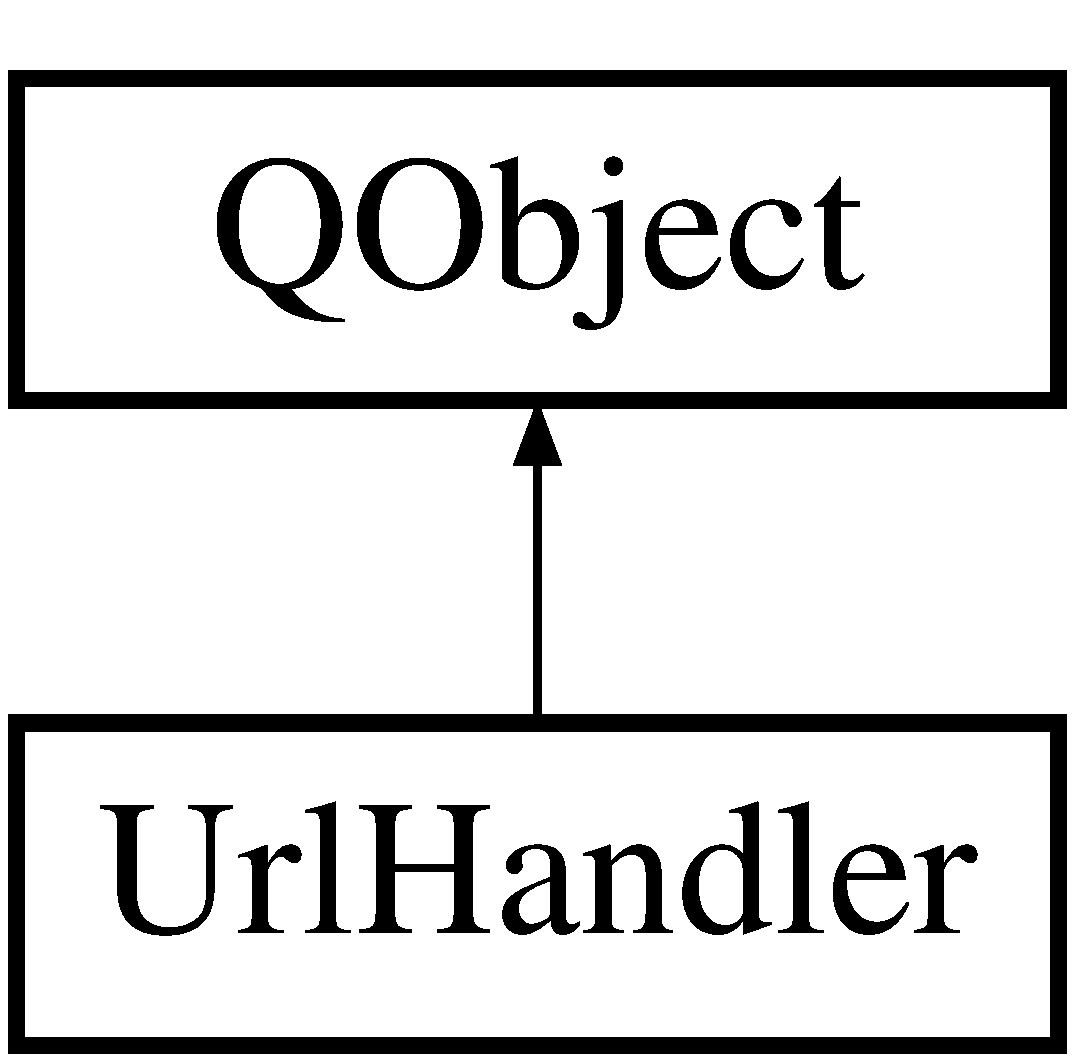
\includegraphics[height=2.000000cm]{class_url_handler}
\end{center}
\end{figure}
\subsection*{Signals}
\begin{DoxyCompactItemize}
\item 
\mbox{\Hypertarget{class_url_handler_a1a519a9fc5c6e07736f430fb02719b4d}\label{class_url_handler_a1a519a9fc5c6e07736f430fb02719b4d}} 
void {\bfseries handle\+Url} (const \hyperlink{class_a_p_i_request}{A\+P\+I\+Request} \&request, \hyperlink{class_a_p_i_response}{A\+P\+I\+Response} $\ast$response)
\end{DoxyCompactItemize}
\subsection*{Public Member Functions}
\begin{DoxyCompactItemize}
\item 
\mbox{\Hypertarget{class_url_handler_a69512a069b2c7e6c74c47ee7894744a0}\label{class_url_handler_a69512a069b2c7e6c74c47ee7894744a0}} 
{\bfseries Url\+Handler} (Q\+Object $\ast$parent)
\item 
\mbox{\Hypertarget{class_url_handler_a2c3f0bc7731a1eb5d732378c3c876043}\label{class_url_handler_a2c3f0bc7731a1eb5d732378c3c876043}} 
\hyperlink{class_a_p_i_response}{A\+P\+I\+Response} {\bfseries handle\+Request} (const \hyperlink{class_a_p_i_request}{A\+P\+I\+Request} \&request)
\end{DoxyCompactItemize}


The documentation for this class was generated from the following file\+:\begin{DoxyCompactItemize}
\item 
L\+C\+S\+Server/Web\+Server.\+h\end{DoxyCompactItemize}

\hypertarget{class_web_server}{}\section{Web\+Server Class Reference}
\label{class_web_server}\index{Web\+Server@{Web\+Server}}


An H\+T\+TP web server implementation that provides the R\+E\+ST A\+PI.  




{\ttfamily \#include $<$Web\+Server.\+h$>$}

Inheritance diagram for Web\+Server\+:\begin{figure}[H]
\begin{center}
\leavevmode
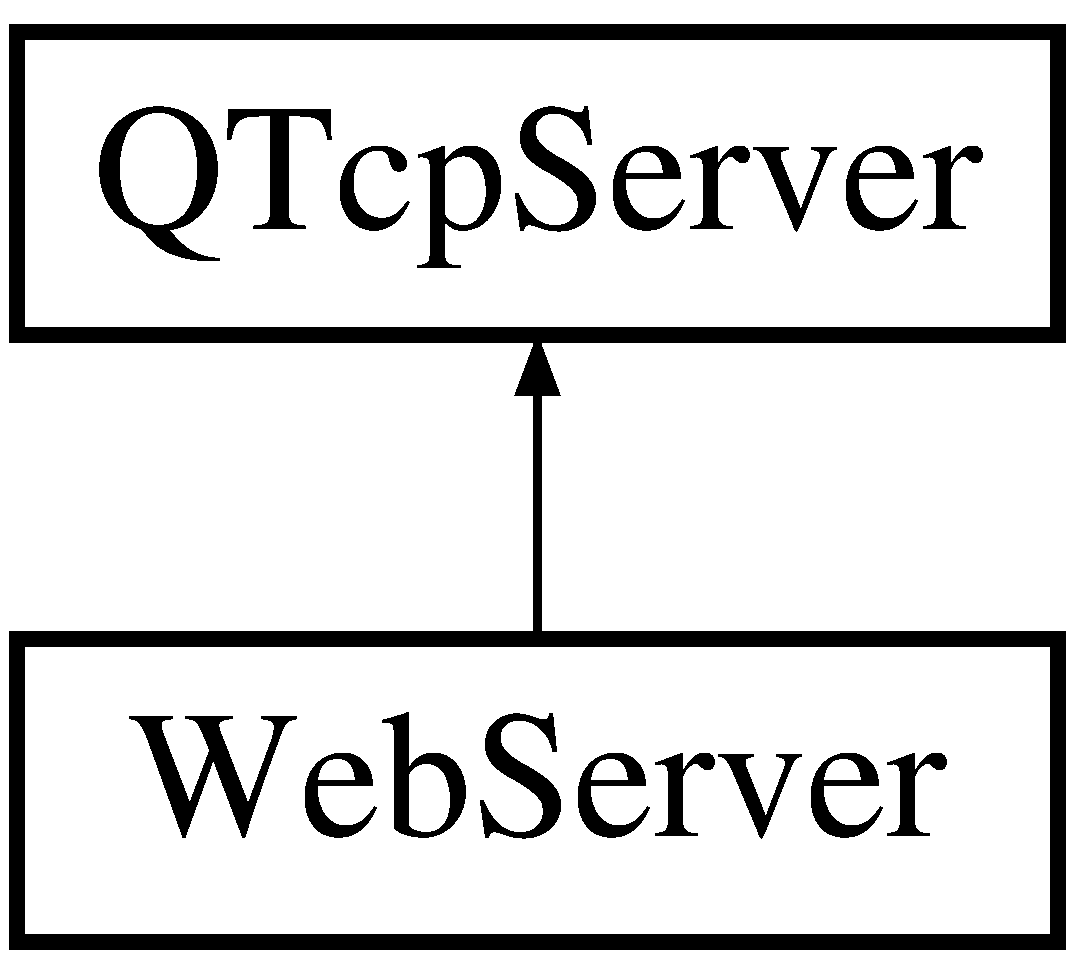
\includegraphics[height=2.000000cm]{class_web_server}
\end{center}
\end{figure}
\subsection*{Public Slots}
\begin{DoxyCompactItemize}
\item 
\mbox{\Hypertarget{class_web_server_a991ba62e7d4044e2f85fe1457aa5bad4}\label{class_web_server_a991ba62e7d4044e2f85fe1457aa5bad4}} 
\hyperlink{class_url_handler}{Url\+Handler} $\ast$ \hyperlink{class_web_server_a991ba62e7d4044e2f85fe1457aa5bad4}{create\+Url\+Handler} (const Q\+String \&path)
\begin{DoxyCompactList}\small\item\em Creates a new \hyperlink{class_url_handler}{Url\+Handler} object and registers the handler for the provided path. \end{DoxyCompactList}\item 
\mbox{\Hypertarget{class_web_server_ac2d1d9d11eb504321fc4629b0e045ce3}\label{class_web_server_ac2d1d9d11eb504321fc4629b0e045ce3}} 
\hyperlink{class_url_handler}{Url\+Handler} $\ast$ \hyperlink{class_web_server_ac2d1d9d11eb504321fc4629b0e045ce3}{get\+Url\+Handler} (const Q\+String \&path)
\begin{DoxyCompactList}\small\item\em Returns the \hyperlink{class_url_handler}{Url\+Handler} object for the given path. N\+U\+LL is returned if a handler for the path is not found. \end{DoxyCompactList}\end{DoxyCompactItemize}
\subsection*{Public Member Functions}
\begin{DoxyCompactItemize}
\item 
\mbox{\Hypertarget{class_web_server_a2902a8136514bc5a1217a87b7a99ab13}\label{class_web_server_a2902a8136514bc5a1217a87b7a99ab13}} 
\hyperlink{class_web_server_a2902a8136514bc5a1217a87b7a99ab13}{Web\+Server} (Q\+Object $\ast$parent=0)
\begin{DoxyCompactList}\small\item\em Constructor. \end{DoxyCompactList}\item 
void \hyperlink{class_web_server_ac6a3155a785e42fec310e8457a12d73e}{incoming\+Connection} (int socket)
\item 
\mbox{\Hypertarget{class_web_server_ad5f434853f45b795976afb32104c03b3}\label{class_web_server_ad5f434853f45b795976afb32104c03b3}} 
void \hyperlink{class_web_server_ad5f434853f45b795976afb32104c03b3}{start\+Server} (quint16 port)
\begin{DoxyCompactList}\small\item\em Starts the server; listening for incoming connections of the provided port. \end{DoxyCompactList}\end{DoxyCompactItemize}
\subsection*{Static Public Member Functions}
\begin{DoxyCompactItemize}
\item 
\mbox{\Hypertarget{class_web_server_a6c77ab01f931f6fed751b2496eec8077}\label{class_web_server_a6c77ab01f931f6fed751b2496eec8077}} 
static \hyperlink{class_web_server}{Web\+Server} $\ast$ \hyperlink{class_web_server_a6c77ab01f931f6fed751b2496eec8077}{instance} (void)
\begin{DoxyCompactList}\small\item\em Returns/creates the singleton instance. \end{DoxyCompactList}\item 
\mbox{\Hypertarget{class_web_server_a99f5239a06368b29ca8bfd6a24be1f98}\label{class_web_server_a99f5239a06368b29ca8bfd6a24be1f98}} 
static Q\+String \hyperlink{class_web_server_a99f5239a06368b29ca8bfd6a24be1f98}{create\+Header} (const Q\+String \&http\+Code, int body\+Size, const Q\+String \&content\+Type=\char`\"{}text/html\char`\"{})
\begin{DoxyCompactList}\small\item\em Creates a standard H\+T\+TP header. \end{DoxyCompactList}\end{DoxyCompactItemize}


\subsection{Detailed Description}
An H\+T\+TP web server implementation that provides the R\+E\+ST A\+PI. 

\hyperlink{class_web_server}{Web\+Server} This class creates an H\+T\+TP web server based on a Q\+Tcp\+Server. Upon a tcp connection, the class looks for a url handler registered through create\+Url\+Handler. If found, the handler\textquotesingle{}s handle\+Request member is called. A \hyperlink{class_url_handler}{Url\+Handler} instance is created by calling \hyperlink{class_web_server_a991ba62e7d4044e2f85fe1457aa5bad4}{Web\+Server\+::create\+Url\+Handler} for a given url. The web server calls the handle\+Request member which emits the handle\+Url signal. 

\subsection{Member Function Documentation}
\mbox{\Hypertarget{class_web_server_ac6a3155a785e42fec310e8457a12d73e}\label{class_web_server_ac6a3155a785e42fec310e8457a12d73e}} 
\index{Web\+Server@{Web\+Server}!incoming\+Connection@{incoming\+Connection}}
\index{incoming\+Connection@{incoming\+Connection}!Web\+Server@{Web\+Server}}
\subsubsection{\texorpdfstring{incoming\+Connection()}{incomingConnection()}}
{\footnotesize\ttfamily void Web\+Server\+::incoming\+Connection (\begin{DoxyParamCaption}\item[{int}]{socket }\end{DoxyParamCaption})}

This virtual function is called by Q\+Tcp\+Server when a new connection is available. The socket\+Descriptor argument is the native socket descriptor for the accepted connection. A new \hyperlink{class_web_server_thread}{Web\+Server\+Thread} object is created which handles the socket request. 

The documentation for this class was generated from the following files\+:\begin{DoxyCompactItemize}
\item 
L\+C\+S\+Server/Web\+Server.\+h\item 
L\+C\+S\+Server/Web\+Server.\+cpp\end{DoxyCompactItemize}

\hypertarget{class_web_server_thread}{}\section{Web\+Server\+Thread Class Reference}
\label{class_web_server_thread}\index{Web\+Server\+Thread@{Web\+Server\+Thread}}


Handles a H\+T\+TP server socket request on a separate thread.  




{\ttfamily \#include $<$Web\+Server\+Thread.\+h$>$}

Inheritance diagram for Web\+Server\+Thread\+:\begin{figure}[H]
\begin{center}
\leavevmode
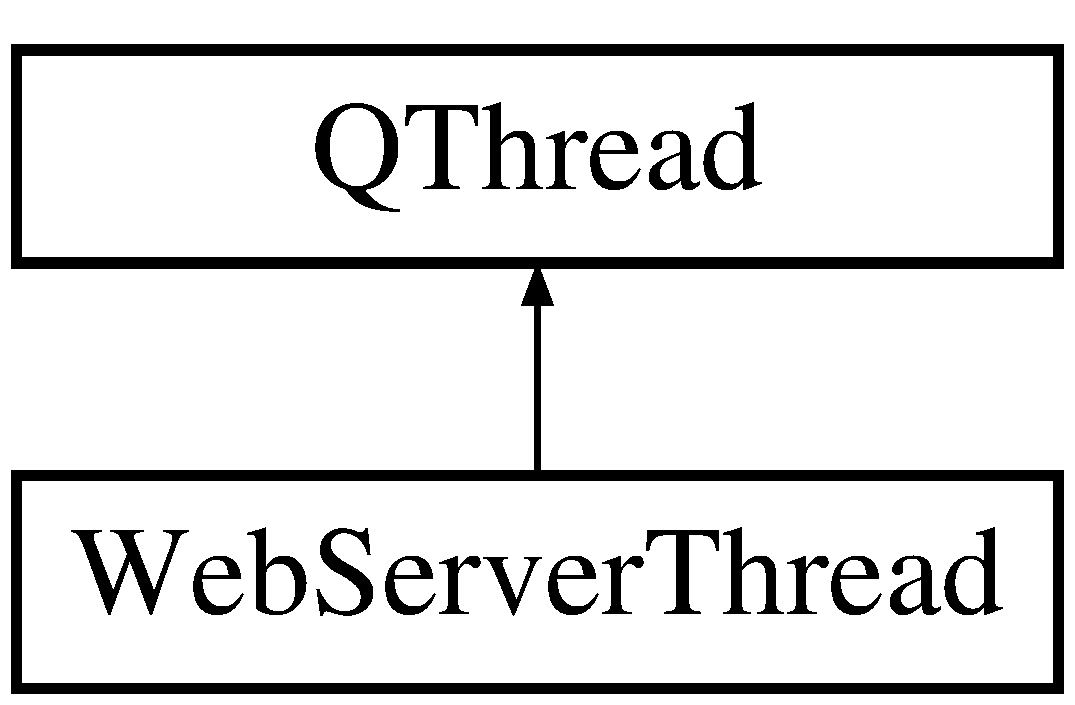
\includegraphics[height=2.000000cm]{class_web_server_thread}
\end{center}
\end{figure}
\subsection*{Public Member Functions}
\begin{DoxyCompactItemize}
\item 
\mbox{\Hypertarget{class_web_server_thread_a1cecaf23741442bf8d58577098d50fc0}\label{class_web_server_thread_a1cecaf23741442bf8d58577098d50fc0}} 
\hyperlink{class_web_server_thread_a1cecaf23741442bf8d58577098d50fc0}{Web\+Server\+Thread} (int m\+\_\+socket\+Descriptor, Q\+Object $\ast$parent)
\begin{DoxyCompactList}\small\item\em Constructor. \end{DoxyCompactList}\item 
\mbox{\Hypertarget{class_web_server_thread_ad8a6737f8667fdc80edde982415ed14d}\label{class_web_server_thread_ad8a6737f8667fdc80edde982415ed14d}} 
\hyperlink{class_web_server_thread_ad8a6737f8667fdc80edde982415ed14d}{$\sim$\+Web\+Server\+Thread} (void)
\begin{DoxyCompactList}\small\item\em Descructor. \end{DoxyCompactList}\item 
\mbox{\Hypertarget{class_web_server_thread_a301c2ed6e2d0c9a020089862e20b7da6}\label{class_web_server_thread_a301c2ed6e2d0c9a020089862e20b7da6}} 
void \hyperlink{class_web_server_thread_a301c2ed6e2d0c9a020089862e20b7da6}{run} ()
\begin{DoxyCompactList}\small\item\em This virtual function is called by Q\+Thread when the thread is started. \end{DoxyCompactList}\end{DoxyCompactItemize}
\subsection*{Protected Slots}
\begin{DoxyCompactItemize}
\item 
\mbox{\Hypertarget{class_web_server_thread_a0f1be6520913476c42b6b7781749af08}\label{class_web_server_thread_a0f1be6520913476c42b6b7781749af08}} 
void {\bfseries ssl\+Errors} (const Q\+List$<$ Q\+Ssl\+Error $>$ \&errors)
\item 
\mbox{\Hypertarget{class_web_server_thread_ab0c66c93e66597e8718a1586543451a1}\label{class_web_server_thread_ab0c66c93e66597e8718a1586543451a1}} 
void {\bfseries socket\+Ready} (void)
\end{DoxyCompactItemize}


\subsection{Detailed Description}
Handles a H\+T\+TP server socket request on a separate thread. 

\hyperlink{class_web_server_thread}{Web\+Server\+Thread} This class creates a Q\+Tcp\+Socket for a given socket descriptor. The run member creates the socket and parses the incoming H\+T\+TP header and attempts to find a \hyperlink{class_url_handler}{Url\+Handler} for the url specified in the H\+T\+TP header. 

The documentation for this class was generated from the following files\+:\begin{DoxyCompactItemize}
\item 
L\+C\+S\+Server/Web\+Server\+Thread.\+h\item 
L\+C\+S\+Server/Web\+Server\+Thread.\+cpp\end{DoxyCompactItemize}

\chapter{File Documentation}
\hypertarget{_global_defs_8h}{}\section{libraries/shared/\+Global\+Defs.h File Reference}
\label{_global_defs_8h}\index{libraries/shared/\+Global\+Defs.\+h@{libraries/shared/\+Global\+Defs.\+h}}
{\ttfamily \#include \char`\"{}Local.\+h\char`\"{}}\newline
\subsection*{Macros}
\begin{DoxyCompactItemize}
\item 
\#define \hyperlink{_global_defs_8h_a88edd2aa4feabff4af21a997d5d8aa23}{D\+E\+B\+U\+G\+\_\+\+P\+R\+I\+NT}(...)~Serial.\+printf( \+\_\+\+\_\+\+V\+A\+\_\+\+A\+R\+G\+S\+\_\+\+\_\+ )
\item 
\#define \hyperlink{_global_defs_8h_acc830d030b46e73bd8c94f0e98aad163}{M\+A\+X\+\_\+\+I2\+C\+\_\+\+R\+E\+T\+RY}~3
\item 
\#define \hyperlink{_global_defs_8h_a90650dd694da82bff003b2c204e30750}{M\+A\+X\+\_\+\+T\+U\+R\+N\+O\+U\+TS}~2
\item 
\#define \hyperlink{_global_defs_8h_a6cce4323245f92154efd90478606fe56}{M\+A\+X\+\_\+\+M\+O\+D\+U\+L\+ES}~8
\item 
\#define \hyperlink{_global_defs_8h_a4e132cfaa78353e3af1474a86b2dd535}{M\+A\+X\+\_\+\+D\+E\+V\+I\+C\+ES}~16
\item 
\#define \hyperlink{_global_defs_8h_a6c6029b8c0bbe5be94fe5a7e5901bae6}{M\+A\+X\+\_\+\+R\+O\+U\+T\+E\+\_\+\+E\+N\+T\+R\+I\+ES}~5
\item 
\#define \hyperlink{_global_defs_8h_ab65c0a5cbe9013d35739fe50345afe4b}{M\+A\+X\+\_\+\+S\+I\+G\+N\+A\+L\+\_\+\+D\+E\+V\+I\+C\+ES}~10
\item 
\#define \hyperlink{_global_defs_8h_a9f90ec2123909529490f97505147b954}{M\+A\+X\+\_\+\+S\+I\+G\+N\+A\+L\+\_\+\+C\+O\+N\+D\+I\+T\+I\+O\+NS}~10
\item 
\#define \hyperlink{_global_defs_8h_a13f06f86104b4525a9429ff04d1c852d}{T\+I\+M\+E\+O\+U\+T\+\_\+\+I\+N\+T\+E\+R\+V\+AL}~200
\item 
\#define \hyperlink{_global_defs_8h_a7f8d257cf2ab673b88ae1307011cbcf5}{H\+E\+A\+R\+T\+B\+E\+A\+T\+\_\+\+I\+N\+T\+E\+R\+V\+AL}~60000
\item 
\#define \hyperlink{_global_defs_8h_a2189cf1afbcd70255e6058334afebdcf}{C\+O\+N\+T\+R\+O\+L\+L\+E\+R\+\_\+\+I\+D\+\_\+\+A\+D\+D\+R\+E\+SS}~7
\item 
\#define \hyperlink{group___u_d_p_message_i_d_gacf1beacf20d9d977b8a27878039d43d7}{T\+R\+N\+\_\+\+S\+T\+A\+T\+US}~1
\item 
\#define \hyperlink{group___u_d_p_message_i_d_gaf8a3426c6f740f351255d50cdda3c9f8}{B\+L\+K\+\_\+\+S\+T\+A\+T\+US}~2
\item 
\#define \hyperlink{group___u_d_p_message_i_d_ga88466ee7861a482c0ebdd16171184747}{D\+E\+V\+I\+C\+E\+\_\+\+S\+T\+A\+T\+US}~3
\item 
\#define \hyperlink{group___u_d_p_message_i_d_gab92fe1aa1c17f0c4e37cf31e79fb1419}{E\+N\+D\+\_\+\+S\+T\+A\+T\+U\+S\+\_\+\+M\+E\+S\+S\+A\+G\+ES}~5
\item 
\#define \hyperlink{group___u_d_p_message_i_d_gab5a0eacfbf0cfab134534d10890d5c25}{T\+R\+N\+\_\+\+A\+C\+T\+I\+V\+A\+TE}~6
\item 
\#define \hyperlink{group___u_d_p_message_i_d_ga44d53121d88631ed14d77f8b6a405816}{T\+R\+N\+\_\+\+A\+C\+T\+I\+V\+A\+T\+E\+\_\+\+R\+O\+U\+TE}~7
\item 
\#define \hyperlink{group___u_d_p_message_i_d_gaf3b0535ed1fed9f9dfb92b18ff78956c}{S\+Y\+S\+\_\+\+A\+CK}~10
\item 
\#define \hyperlink{group___u_d_p_message_i_d_ga23aab89076591390a1dbc412a3a07314}{S\+Y\+S\+\_\+\+C\+O\+N\+T\+R\+O\+L\+L\+E\+R\+\_\+\+O\+N\+L\+I\+NE}~11
\item 
\#define \hyperlink{group___u_d_p_message_i_d_gaddd0be32c40eb5aa6ff7247ec41d402d}{S\+Y\+S\+\_\+\+S\+E\+R\+V\+E\+R\+\_\+\+H\+E\+A\+R\+T\+B\+E\+AT}~12
\item 
\#define \hyperlink{group___u_d_p_message_i_d_ga30863a10d0fcf12b2664d572864c4e0f}{S\+Y\+S\+\_\+\+R\+E\+S\+E\+T\+\_\+\+C\+O\+N\+F\+IG}~13
\item 
\#define \hyperlink{group___u_d_p_message_i_d_gae5a140537bdeb16c6f8ac38ee7a841f6}{S\+Y\+S\+\_\+\+R\+E\+B\+O\+O\+T\+\_\+\+C\+O\+N\+T\+R\+O\+L\+L\+ER}~14
\item 
\#define \hyperlink{group___u_d_p_message_i_d_ga88b6f619a28320e9136847e9b1b27a36}{S\+Y\+S\+\_\+\+D\+O\+W\+N\+L\+O\+A\+D\+\_\+\+F\+I\+R\+M\+W\+A\+RE}~15
\item 
\#define \hyperlink{group___u_d_p_message_i_d_ga9ed42f3a7fcc253fa49ce8ff33a75422}{S\+Y\+S\+\_\+\+R\+E\+S\+T\+A\+R\+T\+I\+NG}~16
\item 
\#define \hyperlink{group___u_d_p_message_i_d_ga596f44c285ab391c72addd0e803b0fc4}{S\+Y\+S\+\_\+\+K\+E\+E\+P\+\_\+\+A\+L\+I\+VE}~18
\item 
\#define \hyperlink{group___u_d_p_message_i_d_gaef042a9ee57e8ddf94286a3263734468}{S\+Y\+S\+\_\+\+R\+E\+S\+E\+T\+\_\+\+D\+E\+V\+I\+C\+E\+\_\+\+C\+O\+N\+F\+IG}~19
\item 
\#define \hyperlink{group___u_d_p_message_i_d_ga3021efce231e9a711d6f498630327086}{S\+Y\+S\+\_\+\+S\+E\+R\+V\+E\+R\+\_\+\+S\+H\+U\+T\+D\+O\+WN}~20
\item 
\#define \hyperlink{group___u_d_p_message_i_d_gadfda0e5a5a6a08de555dd55182a4cd87}{S\+Y\+S\+\_\+\+F\+I\+N\+D\+\_\+\+C\+O\+N\+T\+R\+O\+L\+L\+ER}~21
\item 
\#define \hyperlink{group___u_d_p_message_i_d_gab96f76ffa1af60bebfd871ca1e7c4a08}{S\+Y\+S\+\_\+\+R\+E\+S\+E\+T\+\_\+\+N\+O\+T\+I\+F\+I\+C\+A\+T\+I\+O\+N\+\_\+\+L\+I\+ST}~22
\item 
\#define \hyperlink{group___u_d_p_message_i_d_ga42644954a92421cfe92c2e3d20f795ce}{S\+Y\+S\+\_\+\+L\+O\+C\+K\+\_\+\+D\+E\+V\+I\+CE}~23
\item 
\#define \hyperlink{group___u_d_p_message_i_d_ga9ba07526db57f9ec44d01fe3eba9cc60}{S\+Y\+S\+\_\+\+L\+O\+C\+K\+\_\+\+R\+O\+U\+TE}~24
\end{DoxyCompactItemize}
\subsection*{Enumerations}
\begin{DoxyCompactItemize}
\item 
enum \hyperlink{_global_defs_8h_a51207b6a49e0da6f9978a3019d93480a}{Controller\+Status\+Enum} \{ \newline
\hyperlink{_global_defs_8h_a51207b6a49e0da6f9978a3019d93480aaa27883f1edc134374138cc8c4bf0d647}{Controller\+Status\+Unknown}, 
\hyperlink{_global_defs_8h_a51207b6a49e0da6f9978a3019d93480aabc251fd36725d828139ccffb2a351e43}{Controller\+Status\+Offline}, 
\hyperlink{_global_defs_8h_a51207b6a49e0da6f9978a3019d93480aaf9745934b469024c541b09ce9cd554cf}{Controller\+Status\+Online}, 
\hyperlink{_global_defs_8h_a51207b6a49e0da6f9978a3019d93480aa0bf433e8f26aed75dbc6e39c1ea3e41d}{Controller\+Status\+Restarting}, 
\newline
\hyperlink{_global_defs_8h_a51207b6a49e0da6f9978a3019d93480aac78dbd8bc110021b3d813ccfbcf27d60}{Controller\+Status\+Conected}
 \}\begin{DoxyCompactList}\small\item\em This enum describes the current status of a controller. \end{DoxyCompactList}
\item 
\mbox{\Hypertarget{_global_defs_8h_af309f39f820268e68ac6608068647778}\label{_global_defs_8h_af309f39f820268e68ac6608068647778}} 
enum \hyperlink{_global_defs_8h_af309f39f820268e68ac6608068647778}{Condition\+Connection\+Enum} \{ {\bfseries Connection\+A\+ND}, 
{\bfseries Connection\+OR}
 \}\begin{DoxyCompactList}\small\item\em This enum describes the connection between two condition compares. \end{DoxyCompactList}
\item 
enum \hyperlink{_global_defs_8h_a705748a895b2f4722278227f23819afe}{Condition\+Enum} \{ \hyperlink{_global_defs_8h_a705748a895b2f4722278227f23819afead9d73aa08cbcd6171135769662c94cb6}{Condition\+Equals}, 
\hyperlink{_global_defs_8h_a705748a895b2f4722278227f23819afea5cfe9b940d35bede2caeb94d233000c5}{Condition\+Not\+Equals}
 \}\begin{DoxyCompactList}\small\item\em This enum describes boolean conditional tests used by the Signal device. \end{DoxyCompactList}
\item 
enum \hyperlink{_global_defs_8h_afeb8680eb433d4432e152e3b80c5a3a2}{Pin\+Mode\+Enum} \{ \newline
\hyperlink{_global_defs_8h_afeb8680eb433d4432e152e3b80c5a3a2ae57390ecd33c4a5aec1e944c5d2d6c1f}{Pin\+Unknown}, 
\hyperlink{_global_defs_8h_afeb8680eb433d4432e152e3b80c5a3a2a85b43bb71482d0cfb130e6f6fba3a426}{Pin\+Input}, 
\hyperlink{_global_defs_8h_afeb8680eb433d4432e152e3b80c5a3a2ac8ed66d9b967b24e395a09edb4dd144d}{Pin\+Input\+Pullup}, 
\hyperlink{_global_defs_8h_afeb8680eb433d4432e152e3b80c5a3a2a82f3f58fe43bf727bf2f2b8566e91942}{Pin\+Output}, 
\newline
\hyperlink{_global_defs_8h_afeb8680eb433d4432e152e3b80c5a3a2a8968489528bc28d895e4cd356d0bce82}{Pin\+Output\+Open\+Drain}
 \}\begin{DoxyCompactList}\small\item\em This enum describes input/output configuration of a microchip pin. \end{DoxyCompactList}
\item 
enum \hyperlink{_global_defs_8h_a7a94d683f1fbdeb2365f70c3c286d892}{Pin\+State\+Enum} \{ \hyperlink{_global_defs_8h_a7a94d683f1fbdeb2365f70c3c286d892a1c363c8cb44af216c8e5d4431cd178fa}{Pin\+Off}, 
\hyperlink{_global_defs_8h_a7a94d683f1fbdeb2365f70c3c286d892adb32d253f00defc30254d53d8f25388e}{Pin\+On}, 
\hyperlink{_global_defs_8h_a7a94d683f1fbdeb2365f70c3c286d892a86ff42d0925fe3ab256e008cdc2caf94}{Pin\+Flashing}
 \}\begin{DoxyCompactList}\small\item\em This enum describes current state of a microchip pin. \end{DoxyCompactList}
\item 
\mbox{\Hypertarget{_global_defs_8h_a9ad7563e535f78919ac304b2b0e1109c}\label{_global_defs_8h_a9ad7563e535f78919ac304b2b0e1109c}} 
enum {\bfseries Net\+Action\+Type} \{ {\bfseries Net\+Action\+Get}, 
{\bfseries Net\+Action\+Add}, 
{\bfseries Net\+Action\+Update}, 
{\bfseries Net\+Action\+Delete}
 \}
\item 
enum \hyperlink{_global_defs_8h_aaf453b54a68a7675a75e9149251d2570}{Turnout\+State} \{ \newline
\hyperlink{_global_defs_8h_aaf453b54a68a7675a75e9149251d2570af2de40f5cfb4b41dcc8e5c94d5c77932}{Trn\+Unknown}, 
\hyperlink{_global_defs_8h_aaf453b54a68a7675a75e9149251d2570a7869f1af2f6c7d06e017e663167ade4e}{Trn\+Normal}, 
\hyperlink{_global_defs_8h_aaf453b54a68a7675a75e9149251d2570af2d49320150412cb9ea79428d1381749}{Trn\+To\+Diverging}, 
\hyperlink{_global_defs_8h_aaf453b54a68a7675a75e9149251d2570adee935135c112c031243cb4e7de9a007}{Trn\+Diverging}, 
\newline
\hyperlink{_global_defs_8h_aaf453b54a68a7675a75e9149251d2570ac1cc821561d5dba7f37e0246ae1efaab}{Trn\+To\+Normal}
 \}\begin{DoxyCompactList}\small\item\em This enum describes current state of a Turnout Device. \end{DoxyCompactList}
\item 
enum \hyperlink{_global_defs_8h_ad6cf116f1b761cc66851b7c34eb68d88}{Block\+State} \{ \hyperlink{_global_defs_8h_ad6cf116f1b761cc66851b7c34eb68d88a5268ba75330fb07ad8dbebf5fe1225a2}{Block\+Unknown}, 
\hyperlink{_global_defs_8h_ad6cf116f1b761cc66851b7c34eb68d88a0e7ab0872e100babcf5b57ee44c0116e}{Block\+Clear}, 
\hyperlink{_global_defs_8h_ad6cf116f1b761cc66851b7c34eb68d88a04dbb498a8fb9c4b6e31bc1f877a51d4}{Block\+Occupied}
 \}\begin{DoxyCompactList}\small\item\em This enum describes current state of a Block Detection Device. \end{DoxyCompactList}
\item 
enum \hyperlink{_global_defs_8h_a6ba595014d34f2095b1a55dcf7ae44ea}{Controller\+Class\+Enum} \{ \newline
\hyperlink{_global_defs_8h_a6ba595014d34f2095b1a55dcf7ae44eaa3f29d367cfbb547c1719515f023c085b}{Controller\+Unknown}, 
\hyperlink{_global_defs_8h_a6ba595014d34f2095b1a55dcf7ae44eaac818dfc52be4ff1904c6ad0822a61724}{Controller\+Multi} = 7, 
\hyperlink{_global_defs_8h_a6ba595014d34f2095b1a55dcf7ae44eaaf330e2b5f0738e6030173f694666d9a3}{Controller\+Turnout} = 1, 
\hyperlink{_global_defs_8h_a6ba595014d34f2095b1a55dcf7ae44eaace6f9ad85cb86a0d8a86798d1d99f5dc}{Controller\+Semaphore} = 5, 
\newline
\hyperlink{_global_defs_8h_a6ba595014d34f2095b1a55dcf7ae44eaa2caab087dc9fea0646dc1f85ed30d21e}{Controller\+Server} = 10, 
\hyperlink{_global_defs_8h_a6ba595014d34f2095b1a55dcf7ae44eaa4ab40c9e672caeeeed657924f7b509a2}{Controller\+App}
 \}\begin{DoxyCompactList}\small\item\em This enum describes the classification of a Controller. \end{DoxyCompactList}
\item 
enum \hyperlink{_global_defs_8h_ad17679fac69973be9b3a2787a60d7722}{Device\+Class\+Enum} \{ \newline
\hyperlink{_global_defs_8h_ad17679fac69973be9b3a2787a60d7722a1910d0bd832b02bb63a8d6a80be8cdb6}{Device\+Unknown}, 
\hyperlink{_global_defs_8h_ad17679fac69973be9b3a2787a60d7722a89ff58ae70341de6db9dca8d756644ed}{Device\+Turnout}, 
\hyperlink{_global_defs_8h_ad17679fac69973be9b3a2787a60d7722aabab797056b28bab19aa14ad9bc8b624}{Device\+Panel\+Input}, 
\hyperlink{_global_defs_8h_ad17679fac69973be9b3a2787a60d7722ace5c28add0ed0bbf04dd02f0804d9d08}{Device\+Panel\+Output}, 
\newline
\hyperlink{_global_defs_8h_ad17679fac69973be9b3a2787a60d7722a7e07573bea51a7eacfb2ab240e060839}{Device\+Signal} = 4, 
\hyperlink{_global_defs_8h_ad17679fac69973be9b3a2787a60d7722a66c41faf368824b539ad5abe582bd5a7}{Device\+Semaphore} = 5, 
\hyperlink{_global_defs_8h_ad17679fac69973be9b3a2787a60d7722aa17f9dfdcb84bdb3dc62fab37ae208bb}{Device\+Block} = 6, 
\hyperlink{_global_defs_8h_ad17679fac69973be9b3a2787a60d7722a017113ae14d2c0668cd6103261552acc}{Device\+Panel} = 7
 \}\begin{DoxyCompactList}\small\item\em This enum describes the classification of a Device. \end{DoxyCompactList}
\item 
enum \hyperlink{_global_defs_8h_a60767de316ea8b41147007a892795be3}{Module\+Class\+Enum} \{ \newline
\hyperlink{_global_defs_8h_a60767de316ea8b41147007a892795be3a5fc9c0bd637163bcf805e61d5a2e88cc}{Module\+Unknown}, 
\hyperlink{_global_defs_8h_a60767de316ea8b41147007a892795be3a43107008a6e6e43bc184bcd027c3ad90}{Module\+Turnout} = 1, 
\hyperlink{_global_defs_8h_a60767de316ea8b41147007a892795be3a1d2f6591d598bff4510c9c39bbb1227c}{Module\+Semaphore} = 5, 
\hyperlink{_global_defs_8h_a60767de316ea8b41147007a892795be3ac6a59495f41209d6b4c28fb821cdd9d0}{Module\+Input} = 8, 
\newline
\hyperlink{_global_defs_8h_a60767de316ea8b41147007a892795be3a73bae40ca6b417626a507498e2eabc14}{Module\+Output} = 9
 \}\begin{DoxyCompactList}\small\item\em This enum describes the classification of a Controller Module. \end{DoxyCompactList}
\end{DoxyCompactItemize}
\subsection*{Variables}
\begin{DoxyCompactItemize}
\item 
\mbox{\Hypertarget{_global_defs_8h_a986889658d0597c9527146dd414423a9}\label{_global_defs_8h_a986889658d0597c9527146dd414423a9}} 
const unsigned char {\bfseries Major\+Version} = 3
\item 
\mbox{\Hypertarget{_global_defs_8h_a3c7cecaf45556b9890c37c7e55cd5a78}\label{_global_defs_8h_a3c7cecaf45556b9890c37c7e55cd5a78}} 
const unsigned char {\bfseries Minor\+Version} = 0
\item 
\mbox{\Hypertarget{_global_defs_8h_aca31039db4ec2299dd14f79471999133}\label{_global_defs_8h_aca31039db4ec2299dd14f79471999133}} 
const unsigned char {\bfseries Build\+Version} = 25
\item 
const unsigned char \hyperlink{_global_defs_8h_aef5f1ba5ba8b0f26d0c53dfbe608a365}{Udp\+Broadcast} \mbox{[}$\,$\mbox{]} = \{0x\+F\+F, 0x\+F\+F, 0x\+F\+F, 0x\+F\+F\}
\item 
const unsigned int \hyperlink{_global_defs_8h_af7f2926475cbe113aba0a136e8426649}{Udp\+Port} = 45457
\item 
const unsigned int \hyperlink{_global_defs_8h_a7bcc1cbc2782eefddc126a775d3abab2}{Local\+Server\+Port} = 45455
\end{DoxyCompactItemize}


\subsection{Macro Definition Documentation}
\mbox{\Hypertarget{_global_defs_8h_a2189cf1afbcd70255e6058334afebdcf}\label{_global_defs_8h_a2189cf1afbcd70255e6058334afebdcf}} 
\index{Global\+Defs.\+h@{Global\+Defs.\+h}!C\+O\+N\+T\+R\+O\+L\+L\+E\+R\+\_\+\+I\+D\+\_\+\+A\+D\+D\+R\+E\+SS@{C\+O\+N\+T\+R\+O\+L\+L\+E\+R\+\_\+\+I\+D\+\_\+\+A\+D\+D\+R\+E\+SS}}
\index{C\+O\+N\+T\+R\+O\+L\+L\+E\+R\+\_\+\+I\+D\+\_\+\+A\+D\+D\+R\+E\+SS@{C\+O\+N\+T\+R\+O\+L\+L\+E\+R\+\_\+\+I\+D\+\_\+\+A\+D\+D\+R\+E\+SS}!Global\+Defs.\+h@{Global\+Defs.\+h}}
\subsubsection{\texorpdfstring{C\+O\+N\+T\+R\+O\+L\+L\+E\+R\+\_\+\+I\+D\+\_\+\+A\+D\+D\+R\+E\+SS}{CONTROLLER\_ID\_ADDRESS}}
{\footnotesize\ttfamily \#define C\+O\+N\+T\+R\+O\+L\+L\+E\+R\+\_\+\+I\+D\+\_\+\+A\+D\+D\+R\+E\+SS~7}

Configuration addresses for E\+E\+P\+R\+OM \mbox{\Hypertarget{_global_defs_8h_a88edd2aa4feabff4af21a997d5d8aa23}\label{_global_defs_8h_a88edd2aa4feabff4af21a997d5d8aa23}} 
\index{Global\+Defs.\+h@{Global\+Defs.\+h}!D\+E\+B\+U\+G\+\_\+\+P\+R\+I\+NT@{D\+E\+B\+U\+G\+\_\+\+P\+R\+I\+NT}}
\index{D\+E\+B\+U\+G\+\_\+\+P\+R\+I\+NT@{D\+E\+B\+U\+G\+\_\+\+P\+R\+I\+NT}!Global\+Defs.\+h@{Global\+Defs.\+h}}
\subsubsection{\texorpdfstring{D\+E\+B\+U\+G\+\_\+\+P\+R\+I\+NT}{DEBUG\_PRINT}}
{\footnotesize\ttfamily \#define D\+E\+B\+U\+G\+\_\+\+P\+R\+I\+NT(\begin{DoxyParamCaption}\item[{}]{... }\end{DoxyParamCaption})~Serial.\+printf( \+\_\+\+\_\+\+V\+A\+\_\+\+A\+R\+G\+S\+\_\+\+\_\+ )}

When P\+R\+O\+J\+E\+C\+T\+\_\+\+D\+E\+B\+UG is defined, D\+E\+B\+U\+G\+\_\+\+P\+R\+I\+NT will print output to the serial port. Otherwise, D\+E\+B\+U\+G\+\_\+\+P\+R\+I\+NT does nothing (for release builds) \mbox{\Hypertarget{_global_defs_8h_a7f8d257cf2ab673b88ae1307011cbcf5}\label{_global_defs_8h_a7f8d257cf2ab673b88ae1307011cbcf5}} 
\index{Global\+Defs.\+h@{Global\+Defs.\+h}!H\+E\+A\+R\+T\+B\+E\+A\+T\+\_\+\+I\+N\+T\+E\+R\+V\+AL@{H\+E\+A\+R\+T\+B\+E\+A\+T\+\_\+\+I\+N\+T\+E\+R\+V\+AL}}
\index{H\+E\+A\+R\+T\+B\+E\+A\+T\+\_\+\+I\+N\+T\+E\+R\+V\+AL@{H\+E\+A\+R\+T\+B\+E\+A\+T\+\_\+\+I\+N\+T\+E\+R\+V\+AL}!Global\+Defs.\+h@{Global\+Defs.\+h}}
\subsubsection{\texorpdfstring{H\+E\+A\+R\+T\+B\+E\+A\+T\+\_\+\+I\+N\+T\+E\+R\+V\+AL}{HEARTBEAT\_INTERVAL}}
{\footnotesize\ttfamily \#define H\+E\+A\+R\+T\+B\+E\+A\+T\+\_\+\+I\+N\+T\+E\+R\+V\+AL~60000}

One minute heatbeat broadcast message interval \mbox{\Hypertarget{_global_defs_8h_a4e132cfaa78353e3af1474a86b2dd535}\label{_global_defs_8h_a4e132cfaa78353e3af1474a86b2dd535}} 
\index{Global\+Defs.\+h@{Global\+Defs.\+h}!M\+A\+X\+\_\+\+D\+E\+V\+I\+C\+ES@{M\+A\+X\+\_\+\+D\+E\+V\+I\+C\+ES}}
\index{M\+A\+X\+\_\+\+D\+E\+V\+I\+C\+ES@{M\+A\+X\+\_\+\+D\+E\+V\+I\+C\+ES}!Global\+Defs.\+h@{Global\+Defs.\+h}}
\subsubsection{\texorpdfstring{M\+A\+X\+\_\+\+D\+E\+V\+I\+C\+ES}{MAX\_DEVICES}}
{\footnotesize\ttfamily \#define M\+A\+X\+\_\+\+D\+E\+V\+I\+C\+ES~16}

Total devices per module \mbox{\Hypertarget{_global_defs_8h_acc830d030b46e73bd8c94f0e98aad163}\label{_global_defs_8h_acc830d030b46e73bd8c94f0e98aad163}} 
\index{Global\+Defs.\+h@{Global\+Defs.\+h}!M\+A\+X\+\_\+\+I2\+C\+\_\+\+R\+E\+T\+RY@{M\+A\+X\+\_\+\+I2\+C\+\_\+\+R\+E\+T\+RY}}
\index{M\+A\+X\+\_\+\+I2\+C\+\_\+\+R\+E\+T\+RY@{M\+A\+X\+\_\+\+I2\+C\+\_\+\+R\+E\+T\+RY}!Global\+Defs.\+h@{Global\+Defs.\+h}}
\subsubsection{\texorpdfstring{M\+A\+X\+\_\+\+I2\+C\+\_\+\+R\+E\+T\+RY}{MAX\_I2C\_RETRY}}
{\footnotesize\ttfamily \#define M\+A\+X\+\_\+\+I2\+C\+\_\+\+R\+E\+T\+RY~3}

Maximum I2C B\+US R\+E\+T\+RY C\+O\+U\+NT \mbox{\Hypertarget{_global_defs_8h_a6cce4323245f92154efd90478606fe56}\label{_global_defs_8h_a6cce4323245f92154efd90478606fe56}} 
\index{Global\+Defs.\+h@{Global\+Defs.\+h}!M\+A\+X\+\_\+\+M\+O\+D\+U\+L\+ES@{M\+A\+X\+\_\+\+M\+O\+D\+U\+L\+ES}}
\index{M\+A\+X\+\_\+\+M\+O\+D\+U\+L\+ES@{M\+A\+X\+\_\+\+M\+O\+D\+U\+L\+ES}!Global\+Defs.\+h@{Global\+Defs.\+h}}
\subsubsection{\texorpdfstring{M\+A\+X\+\_\+\+M\+O\+D\+U\+L\+ES}{MAX\_MODULES}}
{\footnotesize\ttfamily \#define M\+A\+X\+\_\+\+M\+O\+D\+U\+L\+ES~8}

Total modules per controller \mbox{\Hypertarget{_global_defs_8h_a6c6029b8c0bbe5be94fe5a7e5901bae6}\label{_global_defs_8h_a6c6029b8c0bbe5be94fe5a7e5901bae6}} 
\index{Global\+Defs.\+h@{Global\+Defs.\+h}!M\+A\+X\+\_\+\+R\+O\+U\+T\+E\+\_\+\+E\+N\+T\+R\+I\+ES@{M\+A\+X\+\_\+\+R\+O\+U\+T\+E\+\_\+\+E\+N\+T\+R\+I\+ES}}
\index{M\+A\+X\+\_\+\+R\+O\+U\+T\+E\+\_\+\+E\+N\+T\+R\+I\+ES@{M\+A\+X\+\_\+\+R\+O\+U\+T\+E\+\_\+\+E\+N\+T\+R\+I\+ES}!Global\+Defs.\+h@{Global\+Defs.\+h}}
\subsubsection{\texorpdfstring{M\+A\+X\+\_\+\+R\+O\+U\+T\+E\+\_\+\+E\+N\+T\+R\+I\+ES}{MAX\_ROUTE\_ENTRIES}}
{\footnotesize\ttfamily \#define M\+A\+X\+\_\+\+R\+O\+U\+T\+E\+\_\+\+E\+N\+T\+R\+I\+ES~5}

Maximum routes a turnout can belong to \mbox{\Hypertarget{_global_defs_8h_a9f90ec2123909529490f97505147b954}\label{_global_defs_8h_a9f90ec2123909529490f97505147b954}} 
\index{Global\+Defs.\+h@{Global\+Defs.\+h}!M\+A\+X\+\_\+\+S\+I\+G\+N\+A\+L\+\_\+\+C\+O\+N\+D\+I\+T\+I\+O\+NS@{M\+A\+X\+\_\+\+S\+I\+G\+N\+A\+L\+\_\+\+C\+O\+N\+D\+I\+T\+I\+O\+NS}}
\index{M\+A\+X\+\_\+\+S\+I\+G\+N\+A\+L\+\_\+\+C\+O\+N\+D\+I\+T\+I\+O\+NS@{M\+A\+X\+\_\+\+S\+I\+G\+N\+A\+L\+\_\+\+C\+O\+N\+D\+I\+T\+I\+O\+NS}!Global\+Defs.\+h@{Global\+Defs.\+h}}
\subsubsection{\texorpdfstring{M\+A\+X\+\_\+\+S\+I\+G\+N\+A\+L\+\_\+\+C\+O\+N\+D\+I\+T\+I\+O\+NS}{MAX\_SIGNAL\_CONDITIONS}}
{\footnotesize\ttfamily \#define M\+A\+X\+\_\+\+S\+I\+G\+N\+A\+L\+\_\+\+C\+O\+N\+D\+I\+T\+I\+O\+NS~10}

Maximum conditions per Signal aspect \mbox{\Hypertarget{_global_defs_8h_ab65c0a5cbe9013d35739fe50345afe4b}\label{_global_defs_8h_ab65c0a5cbe9013d35739fe50345afe4b}} 
\index{Global\+Defs.\+h@{Global\+Defs.\+h}!M\+A\+X\+\_\+\+S\+I\+G\+N\+A\+L\+\_\+\+D\+E\+V\+I\+C\+ES@{M\+A\+X\+\_\+\+S\+I\+G\+N\+A\+L\+\_\+\+D\+E\+V\+I\+C\+ES}}
\index{M\+A\+X\+\_\+\+S\+I\+G\+N\+A\+L\+\_\+\+D\+E\+V\+I\+C\+ES@{M\+A\+X\+\_\+\+S\+I\+G\+N\+A\+L\+\_\+\+D\+E\+V\+I\+C\+ES}!Global\+Defs.\+h@{Global\+Defs.\+h}}
\subsubsection{\texorpdfstring{M\+A\+X\+\_\+\+S\+I\+G\+N\+A\+L\+\_\+\+D\+E\+V\+I\+C\+ES}{MAX\_SIGNAL\_DEVICES}}
{\footnotesize\ttfamily \#define M\+A\+X\+\_\+\+S\+I\+G\+N\+A\+L\+\_\+\+D\+E\+V\+I\+C\+ES~10}

Maximum devices (turnout and blocks) monitored by a Signal device \mbox{\Hypertarget{_global_defs_8h_a90650dd694da82bff003b2c204e30750}\label{_global_defs_8h_a90650dd694da82bff003b2c204e30750}} 
\index{Global\+Defs.\+h@{Global\+Defs.\+h}!M\+A\+X\+\_\+\+T\+U\+R\+N\+O\+U\+TS@{M\+A\+X\+\_\+\+T\+U\+R\+N\+O\+U\+TS}}
\index{M\+A\+X\+\_\+\+T\+U\+R\+N\+O\+U\+TS@{M\+A\+X\+\_\+\+T\+U\+R\+N\+O\+U\+TS}!Global\+Defs.\+h@{Global\+Defs.\+h}}
\subsubsection{\texorpdfstring{M\+A\+X\+\_\+\+T\+U\+R\+N\+O\+U\+TS}{MAX\_TURNOUTS}}
{\footnotesize\ttfamily \#define M\+A\+X\+\_\+\+T\+U\+R\+N\+O\+U\+TS~2}

Total turnouts per module \mbox{\Hypertarget{_global_defs_8h_a13f06f86104b4525a9429ff04d1c852d}\label{_global_defs_8h_a13f06f86104b4525a9429ff04d1c852d}} 
\index{Global\+Defs.\+h@{Global\+Defs.\+h}!T\+I\+M\+E\+O\+U\+T\+\_\+\+I\+N\+T\+E\+R\+V\+AL@{T\+I\+M\+E\+O\+U\+T\+\_\+\+I\+N\+T\+E\+R\+V\+AL}}
\index{T\+I\+M\+E\+O\+U\+T\+\_\+\+I\+N\+T\+E\+R\+V\+AL@{T\+I\+M\+E\+O\+U\+T\+\_\+\+I\+N\+T\+E\+R\+V\+AL}!Global\+Defs.\+h@{Global\+Defs.\+h}}
\subsubsection{\texorpdfstring{T\+I\+M\+E\+O\+U\+T\+\_\+\+I\+N\+T\+E\+R\+V\+AL}{TIMEOUT\_INTERVAL}}
{\footnotesize\ttfamily \#define T\+I\+M\+E\+O\+U\+T\+\_\+\+I\+N\+T\+E\+R\+V\+AL~200}

Input de-\/bounce timeout interval 

\subsection{Enumeration Type Documentation}
\mbox{\Hypertarget{_global_defs_8h_ad6cf116f1b761cc66851b7c34eb68d88}\label{_global_defs_8h_ad6cf116f1b761cc66851b7c34eb68d88}} 
\index{Global\+Defs.\+h@{Global\+Defs.\+h}!Block\+State@{Block\+State}}
\index{Block\+State@{Block\+State}!Global\+Defs.\+h@{Global\+Defs.\+h}}
\subsubsection{\texorpdfstring{Block\+State}{BlockState}}
{\footnotesize\ttfamily enum \hyperlink{_global_defs_8h_ad6cf116f1b761cc66851b7c34eb68d88}{Block\+State}}



This enum describes current state of a Block Detection Device. 

\begin{DoxyEnumFields}{Enumerator}
\raisebox{\heightof{T}}[0pt][0pt]{\index{Block\+Unknown@{Block\+Unknown}!Global\+Defs.\+h@{Global\+Defs.\+h}}\index{Global\+Defs.\+h@{Global\+Defs.\+h}!Block\+Unknown@{Block\+Unknown}}}\mbox{\Hypertarget{_global_defs_8h_ad6cf116f1b761cc66851b7c34eb68d88a5268ba75330fb07ad8dbebf5fe1225a2}\label{_global_defs_8h_ad6cf116f1b761cc66851b7c34eb68d88a5268ba75330fb07ad8dbebf5fe1225a2}} 
Block\+Unknown&The block state cannot be determined. \\
\hline

\raisebox{\heightof{T}}[0pt][0pt]{\index{Block\+Clear@{Block\+Clear}!Global\+Defs.\+h@{Global\+Defs.\+h}}\index{Global\+Defs.\+h@{Global\+Defs.\+h}!Block\+Clear@{Block\+Clear}}}\mbox{\Hypertarget{_global_defs_8h_ad6cf116f1b761cc66851b7c34eb68d88a0e7ab0872e100babcf5b57ee44c0116e}\label{_global_defs_8h_ad6cf116f1b761cc66851b7c34eb68d88a0e7ab0872e100babcf5b57ee44c0116e}} 
Block\+Clear&The block is clear. \\
\hline

\raisebox{\heightof{T}}[0pt][0pt]{\index{Block\+Occupied@{Block\+Occupied}!Global\+Defs.\+h@{Global\+Defs.\+h}}\index{Global\+Defs.\+h@{Global\+Defs.\+h}!Block\+Occupied@{Block\+Occupied}}}\mbox{\Hypertarget{_global_defs_8h_ad6cf116f1b761cc66851b7c34eb68d88a04dbb498a8fb9c4b6e31bc1f877a51d4}\label{_global_defs_8h_ad6cf116f1b761cc66851b7c34eb68d88a04dbb498a8fb9c4b6e31bc1f877a51d4}} 
Block\+Occupied&The block is occupied. \\
\hline

\end{DoxyEnumFields}
\mbox{\Hypertarget{_global_defs_8h_a705748a895b2f4722278227f23819afe}\label{_global_defs_8h_a705748a895b2f4722278227f23819afe}} 
\index{Global\+Defs.\+h@{Global\+Defs.\+h}!Condition\+Enum@{Condition\+Enum}}
\index{Condition\+Enum@{Condition\+Enum}!Global\+Defs.\+h@{Global\+Defs.\+h}}
\subsubsection{\texorpdfstring{Condition\+Enum}{ConditionEnum}}
{\footnotesize\ttfamily enum \hyperlink{_global_defs_8h_a705748a895b2f4722278227f23819afe}{Condition\+Enum}}



This enum describes boolean conditional tests used by the Signal device. 

\begin{DoxyEnumFields}{Enumerator}
\raisebox{\heightof{T}}[0pt][0pt]{\index{Condition\+Equals@{Condition\+Equals}!Global\+Defs.\+h@{Global\+Defs.\+h}}\index{Global\+Defs.\+h@{Global\+Defs.\+h}!Condition\+Equals@{Condition\+Equals}}}\mbox{\Hypertarget{_global_defs_8h_a705748a895b2f4722278227f23819afead9d73aa08cbcd6171135769662c94cb6}\label{_global_defs_8h_a705748a895b2f4722278227f23819afead9d73aa08cbcd6171135769662c94cb6}} 
Condition\+Equals&Compare two values to see if they are equal. \\
\hline

\raisebox{\heightof{T}}[0pt][0pt]{\index{Condition\+Not\+Equals@{Condition\+Not\+Equals}!Global\+Defs.\+h@{Global\+Defs.\+h}}\index{Global\+Defs.\+h@{Global\+Defs.\+h}!Condition\+Not\+Equals@{Condition\+Not\+Equals}}}\mbox{\Hypertarget{_global_defs_8h_a705748a895b2f4722278227f23819afea5cfe9b940d35bede2caeb94d233000c5}\label{_global_defs_8h_a705748a895b2f4722278227f23819afea5cfe9b940d35bede2caeb94d233000c5}} 
Condition\+Not\+Equals&Compare two values to see if they are not equal. \\
\hline

\end{DoxyEnumFields}
\mbox{\Hypertarget{_global_defs_8h_a6ba595014d34f2095b1a55dcf7ae44ea}\label{_global_defs_8h_a6ba595014d34f2095b1a55dcf7ae44ea}} 
\index{Global\+Defs.\+h@{Global\+Defs.\+h}!Controller\+Class\+Enum@{Controller\+Class\+Enum}}
\index{Controller\+Class\+Enum@{Controller\+Class\+Enum}!Global\+Defs.\+h@{Global\+Defs.\+h}}
\subsubsection{\texorpdfstring{Controller\+Class\+Enum}{ControllerClassEnum}}
{\footnotesize\ttfamily enum \hyperlink{_global_defs_8h_a6ba595014d34f2095b1a55dcf7ae44ea}{Controller\+Class\+Enum}}



This enum describes the classification of a Controller. 

\begin{DoxyEnumFields}{Enumerator}
\raisebox{\heightof{T}}[0pt][0pt]{\index{Controller\+Unknown@{Controller\+Unknown}!Global\+Defs.\+h@{Global\+Defs.\+h}}\index{Global\+Defs.\+h@{Global\+Defs.\+h}!Controller\+Unknown@{Controller\+Unknown}}}\mbox{\Hypertarget{_global_defs_8h_a6ba595014d34f2095b1a55dcf7ae44eaa3f29d367cfbb547c1719515f023c085b}\label{_global_defs_8h_a6ba595014d34f2095b1a55dcf7ae44eaa3f29d367cfbb547c1719515f023c085b}} 
Controller\+Unknown&The controller\textquotesingle{}s current classification is unknown. \\
\hline

\raisebox{\heightof{T}}[0pt][0pt]{\index{Controller\+Multi@{Controller\+Multi}!Global\+Defs.\+h@{Global\+Defs.\+h}}\index{Global\+Defs.\+h@{Global\+Defs.\+h}!Controller\+Multi@{Controller\+Multi}}}\mbox{\Hypertarget{_global_defs_8h_a6ba595014d34f2095b1a55dcf7ae44eaac818dfc52be4ff1904c6ad0822a61724}\label{_global_defs_8h_a6ba595014d34f2095b1a55dcf7ae44eaac818dfc52be4ff1904c6ad0822a61724}} 
Controller\+Multi&Multi-\/\+Module Controller. Supports up to 8 devices connected by an I2C serial interface. \\
\hline

\raisebox{\heightof{T}}[0pt][0pt]{\index{Controller\+Turnout@{Controller\+Turnout}!Global\+Defs.\+h@{Global\+Defs.\+h}}\index{Global\+Defs.\+h@{Global\+Defs.\+h}!Controller\+Turnout@{Controller\+Turnout}}}\mbox{\Hypertarget{_global_defs_8h_a6ba595014d34f2095b1a55dcf7ae44eaaf330e2b5f0738e6030173f694666d9a3}\label{_global_defs_8h_a6ba595014d34f2095b1a55dcf7ae44eaaf330e2b5f0738e6030173f694666d9a3}} 
Controller\+Turnout&Turnout Controller which is a Controller + Turnout Module combined on one board. \\
\hline

\raisebox{\heightof{T}}[0pt][0pt]{\index{Controller\+Semaphore@{Controller\+Semaphore}!Global\+Defs.\+h@{Global\+Defs.\+h}}\index{Global\+Defs.\+h@{Global\+Defs.\+h}!Controller\+Semaphore@{Controller\+Semaphore}}}\mbox{\Hypertarget{_global_defs_8h_a6ba595014d34f2095b1a55dcf7ae44eaace6f9ad85cb86a0d8a86798d1d99f5dc}\label{_global_defs_8h_a6ba595014d34f2095b1a55dcf7ae44eaace6f9ad85cb86a0d8a86798d1d99f5dc}} 
Controller\+Semaphore&Semaphore Signal Controller which is a Controller + Turnout module combined on one board. \\
\hline

\raisebox{\heightof{T}}[0pt][0pt]{\index{Controller\+Server@{Controller\+Server}!Global\+Defs.\+h@{Global\+Defs.\+h}}\index{Global\+Defs.\+h@{Global\+Defs.\+h}!Controller\+Server@{Controller\+Server}}}\mbox{\Hypertarget{_global_defs_8h_a6ba595014d34f2095b1a55dcf7ae44eaa2caab087dc9fea0646dc1f85ed30d21e}\label{_global_defs_8h_a6ba595014d34f2095b1a55dcf7ae44eaa2caab087dc9fea0646dc1f85ed30d21e}} 
Controller\+Server&Application Server either a PC desktop or a Raspberry Pi. \\
\hline

\raisebox{\heightof{T}}[0pt][0pt]{\index{Controller\+App@{Controller\+App}!Global\+Defs.\+h@{Global\+Defs.\+h}}\index{Global\+Defs.\+h@{Global\+Defs.\+h}!Controller\+App@{Controller\+App}}}\mbox{\Hypertarget{_global_defs_8h_a6ba595014d34f2095b1a55dcf7ae44eaa4ab40c9e672caeeeed657924f7b509a2}\label{_global_defs_8h_a6ba595014d34f2095b1a55dcf7ae44eaa4ab40c9e672caeeeed657924f7b509a2}} 
Controller\+App&Support/\+Configuration application. \\
\hline

\end{DoxyEnumFields}
\mbox{\Hypertarget{_global_defs_8h_a51207b6a49e0da6f9978a3019d93480a}\label{_global_defs_8h_a51207b6a49e0da6f9978a3019d93480a}} 
\index{Global\+Defs.\+h@{Global\+Defs.\+h}!Controller\+Status\+Enum@{Controller\+Status\+Enum}}
\index{Controller\+Status\+Enum@{Controller\+Status\+Enum}!Global\+Defs.\+h@{Global\+Defs.\+h}}
\subsubsection{\texorpdfstring{Controller\+Status\+Enum}{ControllerStatusEnum}}
{\footnotesize\ttfamily enum \hyperlink{_global_defs_8h_a51207b6a49e0da6f9978a3019d93480a}{Controller\+Status\+Enum}}



This enum describes the current status of a controller. 

\begin{DoxyEnumFields}{Enumerator}
\raisebox{\heightof{T}}[0pt][0pt]{\index{Controller\+Status\+Unknown@{Controller\+Status\+Unknown}!Global\+Defs.\+h@{Global\+Defs.\+h}}\index{Global\+Defs.\+h@{Global\+Defs.\+h}!Controller\+Status\+Unknown@{Controller\+Status\+Unknown}}}\mbox{\Hypertarget{_global_defs_8h_a51207b6a49e0da6f9978a3019d93480aaa27883f1edc134374138cc8c4bf0d647}\label{_global_defs_8h_a51207b6a49e0da6f9978a3019d93480aaa27883f1edc134374138cc8c4bf0d647}} 
Controller\+Status\+Unknown&The controller\textquotesingle{}s current status cannot be determined. \\
\hline

\raisebox{\heightof{T}}[0pt][0pt]{\index{Controller\+Status\+Offline@{Controller\+Status\+Offline}!Global\+Defs.\+h@{Global\+Defs.\+h}}\index{Global\+Defs.\+h@{Global\+Defs.\+h}!Controller\+Status\+Offline@{Controller\+Status\+Offline}}}\mbox{\Hypertarget{_global_defs_8h_a51207b6a49e0da6f9978a3019d93480aabc251fd36725d828139ccffb2a351e43}\label{_global_defs_8h_a51207b6a49e0da6f9978a3019d93480aabc251fd36725d828139ccffb2a351e43}} 
Controller\+Status\+Offline&The controller is offline. \\
\hline

\raisebox{\heightof{T}}[0pt][0pt]{\index{Controller\+Status\+Online@{Controller\+Status\+Online}!Global\+Defs.\+h@{Global\+Defs.\+h}}\index{Global\+Defs.\+h@{Global\+Defs.\+h}!Controller\+Status\+Online@{Controller\+Status\+Online}}}\mbox{\Hypertarget{_global_defs_8h_a51207b6a49e0da6f9978a3019d93480aaf9745934b469024c541b09ce9cd554cf}\label{_global_defs_8h_a51207b6a49e0da6f9978a3019d93480aaf9745934b469024c541b09ce9cd554cf}} 
Controller\+Status\+Online&The controller is online (replaces Controller\+Status\+Connected). \\
\hline

\raisebox{\heightof{T}}[0pt][0pt]{\index{Controller\+Status\+Restarting@{Controller\+Status\+Restarting}!Global\+Defs.\+h@{Global\+Defs.\+h}}\index{Global\+Defs.\+h@{Global\+Defs.\+h}!Controller\+Status\+Restarting@{Controller\+Status\+Restarting}}}\mbox{\Hypertarget{_global_defs_8h_a51207b6a49e0da6f9978a3019d93480aa0bf433e8f26aed75dbc6e39c1ea3e41d}\label{_global_defs_8h_a51207b6a49e0da6f9978a3019d93480aa0bf433e8f26aed75dbc6e39c1ea3e41d}} 
Controller\+Status\+Restarting&The controller is restarting. \\
\hline

\raisebox{\heightof{T}}[0pt][0pt]{\index{Controller\+Status\+Conected@{Controller\+Status\+Conected}!Global\+Defs.\+h@{Global\+Defs.\+h}}\index{Global\+Defs.\+h@{Global\+Defs.\+h}!Controller\+Status\+Conected@{Controller\+Status\+Conected}}}\mbox{\Hypertarget{_global_defs_8h_a51207b6a49e0da6f9978a3019d93480aac78dbd8bc110021b3d813ccfbcf27d60}\label{_global_defs_8h_a51207b6a49e0da6f9978a3019d93480aac78dbd8bc110021b3d813ccfbcf27d60}} 
Controller\+Status\+Conected&No longer used. Kept for backward compatability. \\
\hline

\end{DoxyEnumFields}
\mbox{\Hypertarget{_global_defs_8h_ad17679fac69973be9b3a2787a60d7722}\label{_global_defs_8h_ad17679fac69973be9b3a2787a60d7722}} 
\index{Global\+Defs.\+h@{Global\+Defs.\+h}!Device\+Class\+Enum@{Device\+Class\+Enum}}
\index{Device\+Class\+Enum@{Device\+Class\+Enum}!Global\+Defs.\+h@{Global\+Defs.\+h}}
\subsubsection{\texorpdfstring{Device\+Class\+Enum}{DeviceClassEnum}}
{\footnotesize\ttfamily enum \hyperlink{_global_defs_8h_ad17679fac69973be9b3a2787a60d7722}{Device\+Class\+Enum}}



This enum describes the classification of a Device. 

\begin{DoxyEnumFields}{Enumerator}
\raisebox{\heightof{T}}[0pt][0pt]{\index{Device\+Unknown@{Device\+Unknown}!Global\+Defs.\+h@{Global\+Defs.\+h}}\index{Global\+Defs.\+h@{Global\+Defs.\+h}!Device\+Unknown@{Device\+Unknown}}}\mbox{\Hypertarget{_global_defs_8h_ad17679fac69973be9b3a2787a60d7722a1910d0bd832b02bb63a8d6a80be8cdb6}\label{_global_defs_8h_ad17679fac69973be9b3a2787a60d7722a1910d0bd832b02bb63a8d6a80be8cdb6}} 
Device\+Unknown&The device\textquotesingle{}s current classification is unknown. \\
\hline

\raisebox{\heightof{T}}[0pt][0pt]{\index{Device\+Turnout@{Device\+Turnout}!Global\+Defs.\+h@{Global\+Defs.\+h}}\index{Global\+Defs.\+h@{Global\+Defs.\+h}!Device\+Turnout@{Device\+Turnout}}}\mbox{\Hypertarget{_global_defs_8h_ad17679fac69973be9b3a2787a60d7722a89ff58ae70341de6db9dca8d756644ed}\label{_global_defs_8h_ad17679fac69973be9b3a2787a60d7722a89ff58ae70341de6db9dca8d756644ed}} 
Device\+Turnout&Turnout Device. \\
\hline

\raisebox{\heightof{T}}[0pt][0pt]{\index{Device\+Panel\+Input@{Device\+Panel\+Input}!Global\+Defs.\+h@{Global\+Defs.\+h}}\index{Global\+Defs.\+h@{Global\+Defs.\+h}!Device\+Panel\+Input@{Device\+Panel\+Input}}}\mbox{\Hypertarget{_global_defs_8h_ad17679fac69973be9b3a2787a60d7722aabab797056b28bab19aa14ad9bc8b624}\label{_global_defs_8h_ad17679fac69973be9b3a2787a60d7722aabab797056b28bab19aa14ad9bc8b624}} 
Device\+Panel\+Input&Panel Button Input device. \\
\hline

\raisebox{\heightof{T}}[0pt][0pt]{\index{Device\+Panel\+Output@{Device\+Panel\+Output}!Global\+Defs.\+h@{Global\+Defs.\+h}}\index{Global\+Defs.\+h@{Global\+Defs.\+h}!Device\+Panel\+Output@{Device\+Panel\+Output}}}\mbox{\Hypertarget{_global_defs_8h_ad17679fac69973be9b3a2787a60d7722ace5c28add0ed0bbf04dd02f0804d9d08}\label{_global_defs_8h_ad17679fac69973be9b3a2787a60d7722ace5c28add0ed0bbf04dd02f0804d9d08}} 
Device\+Panel\+Output&Panel L\+ED Output Module. \\
\hline

\raisebox{\heightof{T}}[0pt][0pt]{\index{Device\+Signal@{Device\+Signal}!Global\+Defs.\+h@{Global\+Defs.\+h}}\index{Global\+Defs.\+h@{Global\+Defs.\+h}!Device\+Signal@{Device\+Signal}}}\mbox{\Hypertarget{_global_defs_8h_ad17679fac69973be9b3a2787a60d7722a7e07573bea51a7eacfb2ab240e060839}\label{_global_defs_8h_ad17679fac69973be9b3a2787a60d7722a7e07573bea51a7eacfb2ab240e060839}} 
Device\+Signal&Signal Device. \\
\hline

\raisebox{\heightof{T}}[0pt][0pt]{\index{Device\+Semaphore@{Device\+Semaphore}!Global\+Defs.\+h@{Global\+Defs.\+h}}\index{Global\+Defs.\+h@{Global\+Defs.\+h}!Device\+Semaphore@{Device\+Semaphore}}}\mbox{\Hypertarget{_global_defs_8h_ad17679fac69973be9b3a2787a60d7722a66c41faf368824b539ad5abe582bd5a7}\label{_global_defs_8h_ad17679fac69973be9b3a2787a60d7722a66c41faf368824b539ad5abe582bd5a7}} 
Device\+Semaphore&Semaphore Signal Device. \\
\hline

\raisebox{\heightof{T}}[0pt][0pt]{\index{Device\+Block@{Device\+Block}!Global\+Defs.\+h@{Global\+Defs.\+h}}\index{Global\+Defs.\+h@{Global\+Defs.\+h}!Device\+Block@{Device\+Block}}}\mbox{\Hypertarget{_global_defs_8h_ad17679fac69973be9b3a2787a60d7722aa17f9dfdcb84bdb3dc62fab37ae208bb}\label{_global_defs_8h_ad17679fac69973be9b3a2787a60d7722aa17f9dfdcb84bdb3dc62fab37ae208bb}} 
Device\+Block&Block Device. \\
\hline

\raisebox{\heightof{T}}[0pt][0pt]{\index{Device\+Panel@{Device\+Panel}!Global\+Defs.\+h@{Global\+Defs.\+h}}\index{Global\+Defs.\+h@{Global\+Defs.\+h}!Device\+Panel@{Device\+Panel}}}\mbox{\Hypertarget{_global_defs_8h_ad17679fac69973be9b3a2787a60d7722a017113ae14d2c0668cd6103261552acc}\label{_global_defs_8h_ad17679fac69973be9b3a2787a60d7722a017113ae14d2c0668cd6103261552acc}} 
Device\+Panel&For older versions--no longer used. \\
\hline

\end{DoxyEnumFields}
\mbox{\Hypertarget{_global_defs_8h_a60767de316ea8b41147007a892795be3}\label{_global_defs_8h_a60767de316ea8b41147007a892795be3}} 
\index{Global\+Defs.\+h@{Global\+Defs.\+h}!Module\+Class\+Enum@{Module\+Class\+Enum}}
\index{Module\+Class\+Enum@{Module\+Class\+Enum}!Global\+Defs.\+h@{Global\+Defs.\+h}}
\subsubsection{\texorpdfstring{Module\+Class\+Enum}{ModuleClassEnum}}
{\footnotesize\ttfamily enum \hyperlink{_global_defs_8h_a60767de316ea8b41147007a892795be3}{Module\+Class\+Enum}}



This enum describes the classification of a Controller Module. 

\begin{DoxyEnumFields}{Enumerator}
\raisebox{\heightof{T}}[0pt][0pt]{\index{Module\+Unknown@{Module\+Unknown}!Global\+Defs.\+h@{Global\+Defs.\+h}}\index{Global\+Defs.\+h@{Global\+Defs.\+h}!Module\+Unknown@{Module\+Unknown}}}\mbox{\Hypertarget{_global_defs_8h_a60767de316ea8b41147007a892795be3a5fc9c0bd637163bcf805e61d5a2e88cc}\label{_global_defs_8h_a60767de316ea8b41147007a892795be3a5fc9c0bd637163bcf805e61d5a2e88cc}} 
Module\+Unknown&The controller module\textquotesingle{}s current classification is unknown. \\
\hline

\raisebox{\heightof{T}}[0pt][0pt]{\index{Module\+Turnout@{Module\+Turnout}!Global\+Defs.\+h@{Global\+Defs.\+h}}\index{Global\+Defs.\+h@{Global\+Defs.\+h}!Module\+Turnout@{Module\+Turnout}}}\mbox{\Hypertarget{_global_defs_8h_a60767de316ea8b41147007a892795be3a43107008a6e6e43bc184bcd027c3ad90}\label{_global_defs_8h_a60767de316ea8b41147007a892795be3a43107008a6e6e43bc184bcd027c3ad90}} 
Module\+Turnout&Turnout Module. \\
\hline

\raisebox{\heightof{T}}[0pt][0pt]{\index{Module\+Semaphore@{Module\+Semaphore}!Global\+Defs.\+h@{Global\+Defs.\+h}}\index{Global\+Defs.\+h@{Global\+Defs.\+h}!Module\+Semaphore@{Module\+Semaphore}}}\mbox{\Hypertarget{_global_defs_8h_a60767de316ea8b41147007a892795be3a1d2f6591d598bff4510c9c39bbb1227c}\label{_global_defs_8h_a60767de316ea8b41147007a892795be3a1d2f6591d598bff4510c9c39bbb1227c}} 
Module\+Semaphore&Semaphore Module which is really a turnout module. \\
\hline

\raisebox{\heightof{T}}[0pt][0pt]{\index{Module\+Input@{Module\+Input}!Global\+Defs.\+h@{Global\+Defs.\+h}}\index{Global\+Defs.\+h@{Global\+Defs.\+h}!Module\+Input@{Module\+Input}}}\mbox{\Hypertarget{_global_defs_8h_a60767de316ea8b41147007a892795be3ac6a59495f41209d6b4c28fb821cdd9d0}\label{_global_defs_8h_a60767de316ea8b41147007a892795be3ac6a59495f41209d6b4c28fb821cdd9d0}} 
Module\+Input&Input Module used by Panel Input and Block devices. \\
\hline

\raisebox{\heightof{T}}[0pt][0pt]{\index{Module\+Output@{Module\+Output}!Global\+Defs.\+h@{Global\+Defs.\+h}}\index{Global\+Defs.\+h@{Global\+Defs.\+h}!Module\+Output@{Module\+Output}}}\mbox{\Hypertarget{_global_defs_8h_a60767de316ea8b41147007a892795be3a73bae40ca6b417626a507498e2eabc14}\label{_global_defs_8h_a60767de316ea8b41147007a892795be3a73bae40ca6b417626a507498e2eabc14}} 
Module\+Output&Output Module used by Panel Output and Signal devices. \\
\hline

\end{DoxyEnumFields}
\mbox{\Hypertarget{_global_defs_8h_afeb8680eb433d4432e152e3b80c5a3a2}\label{_global_defs_8h_afeb8680eb433d4432e152e3b80c5a3a2}} 
\index{Global\+Defs.\+h@{Global\+Defs.\+h}!Pin\+Mode\+Enum@{Pin\+Mode\+Enum}}
\index{Pin\+Mode\+Enum@{Pin\+Mode\+Enum}!Global\+Defs.\+h@{Global\+Defs.\+h}}
\subsubsection{\texorpdfstring{Pin\+Mode\+Enum}{PinModeEnum}}
{\footnotesize\ttfamily enum \hyperlink{_global_defs_8h_afeb8680eb433d4432e152e3b80c5a3a2}{Pin\+Mode\+Enum}}



This enum describes input/output configuration of a microchip pin. 

\begin{DoxyEnumFields}{Enumerator}
\raisebox{\heightof{T}}[0pt][0pt]{\index{Pin\+Unknown@{Pin\+Unknown}!Global\+Defs.\+h@{Global\+Defs.\+h}}\index{Global\+Defs.\+h@{Global\+Defs.\+h}!Pin\+Unknown@{Pin\+Unknown}}}\mbox{\Hypertarget{_global_defs_8h_afeb8680eb433d4432e152e3b80c5a3a2ae57390ecd33c4a5aec1e944c5d2d6c1f}\label{_global_defs_8h_afeb8680eb433d4432e152e3b80c5a3a2ae57390ecd33c4a5aec1e944c5d2d6c1f}} 
Pin\+Unknown&The pin mode cannot be determined. \\
\hline

\raisebox{\heightof{T}}[0pt][0pt]{\index{Pin\+Input@{Pin\+Input}!Global\+Defs.\+h@{Global\+Defs.\+h}}\index{Global\+Defs.\+h@{Global\+Defs.\+h}!Pin\+Input@{Pin\+Input}}}\mbox{\Hypertarget{_global_defs_8h_afeb8680eb433d4432e152e3b80c5a3a2a85b43bb71482d0cfb130e6f6fba3a426}\label{_global_defs_8h_afeb8680eb433d4432e152e3b80c5a3a2a85b43bb71482d0cfb130e6f6fba3a426}} 
Pin\+Input&The pin is set to input mode. \\
\hline

\raisebox{\heightof{T}}[0pt][0pt]{\index{Pin\+Input\+Pullup@{Pin\+Input\+Pullup}!Global\+Defs.\+h@{Global\+Defs.\+h}}\index{Global\+Defs.\+h@{Global\+Defs.\+h}!Pin\+Input\+Pullup@{Pin\+Input\+Pullup}}}\mbox{\Hypertarget{_global_defs_8h_afeb8680eb433d4432e152e3b80c5a3a2ac8ed66d9b967b24e395a09edb4dd144d}\label{_global_defs_8h_afeb8680eb433d4432e152e3b80c5a3a2ac8ed66d9b967b24e395a09edb4dd144d}} 
Pin\+Input\+Pullup&The pin is set to input mode using the internal pull-\/up resistor. \\
\hline

\raisebox{\heightof{T}}[0pt][0pt]{\index{Pin\+Output@{Pin\+Output}!Global\+Defs.\+h@{Global\+Defs.\+h}}\index{Global\+Defs.\+h@{Global\+Defs.\+h}!Pin\+Output@{Pin\+Output}}}\mbox{\Hypertarget{_global_defs_8h_afeb8680eb433d4432e152e3b80c5a3a2a82f3f58fe43bf727bf2f2b8566e91942}\label{_global_defs_8h_afeb8680eb433d4432e152e3b80c5a3a2a82f3f58fe43bf727bf2f2b8566e91942}} 
Pin\+Output&The pin is set to output mode. \\
\hline

\raisebox{\heightof{T}}[0pt][0pt]{\index{Pin\+Output\+Open\+Drain@{Pin\+Output\+Open\+Drain}!Global\+Defs.\+h@{Global\+Defs.\+h}}\index{Global\+Defs.\+h@{Global\+Defs.\+h}!Pin\+Output\+Open\+Drain@{Pin\+Output\+Open\+Drain}}}\mbox{\Hypertarget{_global_defs_8h_afeb8680eb433d4432e152e3b80c5a3a2a8968489528bc28d895e4cd356d0bce82}\label{_global_defs_8h_afeb8680eb433d4432e152e3b80c5a3a2a8968489528bc28d895e4cd356d0bce82}} 
Pin\+Output\+Open\+Drain&The pin is set to output mode. \\
\hline

\end{DoxyEnumFields}
\mbox{\Hypertarget{_global_defs_8h_a7a94d683f1fbdeb2365f70c3c286d892}\label{_global_defs_8h_a7a94d683f1fbdeb2365f70c3c286d892}} 
\index{Global\+Defs.\+h@{Global\+Defs.\+h}!Pin\+State\+Enum@{Pin\+State\+Enum}}
\index{Pin\+State\+Enum@{Pin\+State\+Enum}!Global\+Defs.\+h@{Global\+Defs.\+h}}
\subsubsection{\texorpdfstring{Pin\+State\+Enum}{PinStateEnum}}
{\footnotesize\ttfamily enum \hyperlink{_global_defs_8h_a7a94d683f1fbdeb2365f70c3c286d892}{Pin\+State\+Enum}}



This enum describes current state of a microchip pin. 

\begin{DoxyEnumFields}{Enumerator}
\raisebox{\heightof{T}}[0pt][0pt]{\index{Pin\+Off@{Pin\+Off}!Global\+Defs.\+h@{Global\+Defs.\+h}}\index{Global\+Defs.\+h@{Global\+Defs.\+h}!Pin\+Off@{Pin\+Off}}}\mbox{\Hypertarget{_global_defs_8h_a7a94d683f1fbdeb2365f70c3c286d892a1c363c8cb44af216c8e5d4431cd178fa}\label{_global_defs_8h_a7a94d683f1fbdeb2365f70c3c286d892a1c363c8cb44af216c8e5d4431cd178fa}} 
Pin\+Off&The pin is off (L\+OW). \\
\hline

\raisebox{\heightof{T}}[0pt][0pt]{\index{Pin\+On@{Pin\+On}!Global\+Defs.\+h@{Global\+Defs.\+h}}\index{Global\+Defs.\+h@{Global\+Defs.\+h}!Pin\+On@{Pin\+On}}}\mbox{\Hypertarget{_global_defs_8h_a7a94d683f1fbdeb2365f70c3c286d892adb32d253f00defc30254d53d8f25388e}\label{_global_defs_8h_a7a94d683f1fbdeb2365f70c3c286d892adb32d253f00defc30254d53d8f25388e}} 
Pin\+On&The pin is on (H\+I\+GH). \\
\hline

\raisebox{\heightof{T}}[0pt][0pt]{\index{Pin\+Flashing@{Pin\+Flashing}!Global\+Defs.\+h@{Global\+Defs.\+h}}\index{Global\+Defs.\+h@{Global\+Defs.\+h}!Pin\+Flashing@{Pin\+Flashing}}}\mbox{\Hypertarget{_global_defs_8h_a7a94d683f1fbdeb2365f70c3c286d892a86ff42d0925fe3ab256e008cdc2caf94}\label{_global_defs_8h_a7a94d683f1fbdeb2365f70c3c286d892a86ff42d0925fe3ab256e008cdc2caf94}} 
Pin\+Flashing&The pin is set to alternate between on and off (L\+OW and H\+I\+GH) states at a timed interval. \\
\hline

\end{DoxyEnumFields}
\mbox{\Hypertarget{_global_defs_8h_aaf453b54a68a7675a75e9149251d2570}\label{_global_defs_8h_aaf453b54a68a7675a75e9149251d2570}} 
\index{Global\+Defs.\+h@{Global\+Defs.\+h}!Turnout\+State@{Turnout\+State}}
\index{Turnout\+State@{Turnout\+State}!Global\+Defs.\+h@{Global\+Defs.\+h}}
\subsubsection{\texorpdfstring{Turnout\+State}{TurnoutState}}
{\footnotesize\ttfamily enum \hyperlink{_global_defs_8h_aaf453b54a68a7675a75e9149251d2570}{Turnout\+State}}



This enum describes current state of a Turnout Device. 

\begin{DoxyEnumFields}{Enumerator}
\raisebox{\heightof{T}}[0pt][0pt]{\index{Trn\+Unknown@{Trn\+Unknown}!Global\+Defs.\+h@{Global\+Defs.\+h}}\index{Global\+Defs.\+h@{Global\+Defs.\+h}!Trn\+Unknown@{Trn\+Unknown}}}\mbox{\Hypertarget{_global_defs_8h_aaf453b54a68a7675a75e9149251d2570af2de40f5cfb4b41dcc8e5c94d5c77932}\label{_global_defs_8h_aaf453b54a68a7675a75e9149251d2570af2de40f5cfb4b41dcc8e5c94d5c77932}} 
Trn\+Unknown&The turnout state cannot be determined. \\
\hline

\raisebox{\heightof{T}}[0pt][0pt]{\index{Trn\+Normal@{Trn\+Normal}!Global\+Defs.\+h@{Global\+Defs.\+h}}\index{Global\+Defs.\+h@{Global\+Defs.\+h}!Trn\+Normal@{Trn\+Normal}}}\mbox{\Hypertarget{_global_defs_8h_aaf453b54a68a7675a75e9149251d2570a7869f1af2f6c7d06e017e663167ade4e}\label{_global_defs_8h_aaf453b54a68a7675a75e9149251d2570a7869f1af2f6c7d06e017e663167ade4e}} 
Trn\+Normal&The turnout is set to it\textquotesingle{}s normal route (usually the straight direction). \\
\hline

\raisebox{\heightof{T}}[0pt][0pt]{\index{Trn\+To\+Diverging@{Trn\+To\+Diverging}!Global\+Defs.\+h@{Global\+Defs.\+h}}\index{Global\+Defs.\+h@{Global\+Defs.\+h}!Trn\+To\+Diverging@{Trn\+To\+Diverging}}}\mbox{\Hypertarget{_global_defs_8h_aaf453b54a68a7675a75e9149251d2570af2d49320150412cb9ea79428d1381749}\label{_global_defs_8h_aaf453b54a68a7675a75e9149251d2570af2d49320150412cb9ea79428d1381749}} 
Trn\+To\+Diverging&The turnout is in motion, changing from the normal route to the diverging route. \\
\hline

\raisebox{\heightof{T}}[0pt][0pt]{\index{Trn\+Diverging@{Trn\+Diverging}!Global\+Defs.\+h@{Global\+Defs.\+h}}\index{Global\+Defs.\+h@{Global\+Defs.\+h}!Trn\+Diverging@{Trn\+Diverging}}}\mbox{\Hypertarget{_global_defs_8h_aaf453b54a68a7675a75e9149251d2570adee935135c112c031243cb4e7de9a007}\label{_global_defs_8h_aaf453b54a68a7675a75e9149251d2570adee935135c112c031243cb4e7de9a007}} 
Trn\+Diverging&The turnout is set to the diverging route. \\
\hline

\raisebox{\heightof{T}}[0pt][0pt]{\index{Trn\+To\+Normal@{Trn\+To\+Normal}!Global\+Defs.\+h@{Global\+Defs.\+h}}\index{Global\+Defs.\+h@{Global\+Defs.\+h}!Trn\+To\+Normal@{Trn\+To\+Normal}}}\mbox{\Hypertarget{_global_defs_8h_aaf453b54a68a7675a75e9149251d2570ac1cc821561d5dba7f37e0246ae1efaab}\label{_global_defs_8h_aaf453b54a68a7675a75e9149251d2570ac1cc821561d5dba7f37e0246ae1efaab}} 
Trn\+To\+Normal&The turnout is in motion, changing from the diverging route to the normal route. \\
\hline

\end{DoxyEnumFields}


\subsection{Variable Documentation}
\mbox{\Hypertarget{_global_defs_8h_a7bcc1cbc2782eefddc126a775d3abab2}\label{_global_defs_8h_a7bcc1cbc2782eefddc126a775d3abab2}} 
\index{Global\+Defs.\+h@{Global\+Defs.\+h}!Local\+Server\+Port@{Local\+Server\+Port}}
\index{Local\+Server\+Port@{Local\+Server\+Port}!Global\+Defs.\+h@{Global\+Defs.\+h}}
\subsubsection{\texorpdfstring{Local\+Server\+Port}{LocalServerPort}}
{\footnotesize\ttfamily const unsigned int Local\+Server\+Port = 45455}

Local (controller) http server port. Reserved for future use. \mbox{\Hypertarget{_global_defs_8h_aef5f1ba5ba8b0f26d0c53dfbe608a365}\label{_global_defs_8h_aef5f1ba5ba8b0f26d0c53dfbe608a365}} 
\index{Global\+Defs.\+h@{Global\+Defs.\+h}!Udp\+Broadcast@{Udp\+Broadcast}}
\index{Udp\+Broadcast@{Udp\+Broadcast}!Global\+Defs.\+h@{Global\+Defs.\+h}}
\subsubsection{\texorpdfstring{Udp\+Broadcast}{UdpBroadcast}}
{\footnotesize\ttfamily const unsigned char Udp\+Broadcast\mbox{[}$\,$\mbox{]} = \{0x\+F\+F, 0x\+F\+F, 0x\+F\+F, 0x\+F\+F\}}

U\+DP broadcast address \mbox{\Hypertarget{_global_defs_8h_af7f2926475cbe113aba0a136e8426649}\label{_global_defs_8h_af7f2926475cbe113aba0a136e8426649}} 
\index{Global\+Defs.\+h@{Global\+Defs.\+h}!Udp\+Port@{Udp\+Port}}
\index{Udp\+Port@{Udp\+Port}!Global\+Defs.\+h@{Global\+Defs.\+h}}
\subsubsection{\texorpdfstring{Udp\+Port}{UdpPort}}
{\footnotesize\ttfamily const unsigned int Udp\+Port = 45457}

U\+DP port 
%--- End generated contents ---

% Index
\backmatter
\newpage
\phantomsection
\clearemptydoublepage
\addcontentsline{toc}{chapter}{Index}
\printindex

\end{document}
